\pagestyle{empty}
\phantom{A}
\vfill
\centerline{\rule{0.8\textwidth}{0.5ex}}
\hrule
\vskip 3mm
\centerline{\Large\bfseries\sc Optimalizácia a aproximácia}
\vskip 3mm
\hrule
\centerline{\rule{0.8\textwidth}{0.5ex}}
\vfill
Rasťo Královič\hfill (predbežná $\alpha$ verzia)  \hfill \today
\newpage
\phantom{A}
\newpage
\section*{O čom je tento text}

\noindent
Text je prevažne kompilátom z viacerých kníh (najmä \cite{GLS88},\cite{MG07},\cite{V04},\cite{WS11}),
článkov, poznámok z prednášok a prezentácií.


\vfill\noindent
Tento text vznikol ako študijný materiál ku kuru\\
{\em 2-INF-221: Aproximácia optimalizačných problémov} \\
na FMFI UK.


V texte je použitá grafika: \\
\begin{itemize}
  \item unit sprites from the project ''Battle for Wesnoth'' {\tt http://www.wesnoth.org}
  \item binder graphics from the project digstud {\tt https://github.com/bitfragment/digstud.git}
  \item images of printers from manufacturers' web presentations
\end{itemize}


\newpage
\tableofcontents
\newpage
\setcounter{page}{1}
\pagestyle{plain}

\typeout{EEEEEEEEEEEEE \thepage EEEEEEEEEEEEEEEEE}
\chapter{Aproximačné algoritmy}
Predpokladáme, že čitateľ pozná techniky návrhu efektívnych algoritmov a
stretol sa s analýzou ich časovej zložitosti. Je tiež užitočné, ak má predstavu
o základoch teórie zložitosti, aj keď nateraz nám bude stačiť, že za efektívne
riešiteľné považujeme tie problémy, pre ktoré existuje polynomiálny algoritmus
(t.j. algoritmus, ktorý pre každý vstup vráti správny výstup a jeho čas behu je
ohraničený polynómom od veľkosti vstupu) a že existuje veľa problémov, pre
ktoré žiaden takýto algoritmus nepoznáme. 

V nasledujúcom texte pokračujeme z tohoto východiska. Budeme sa, až na zopár
výnimiek, zaoberať problémami, pre ktoré nepoznáme polynomiálny algoritmus, a
napriek tomu by sme ich chceli nejako efektívne riešiť. Prijmeme tézu, že 
efektívne riešenie musí byť v polynomiálnom čase, a preto v ďalšom texte budeme,
okrem prípadov, keď vyslovene povieme inak, za {\em algoritmus} považovať
{\em algoritmus pracujúci v polynomiálnom čase}.
Budeme skúmať jeden z možných
prístupov: ak už nevieme spraviť algoritmus, ktorý vždy vráti
správne riešenie, možno by sme sa dokázali uspokojiť s 
algoritmom, ktorý vždy nájde ''takmer správne'' riešenie. Toto,
samozrejme, závisí od typu problému.  Napr. pre rozhodovacie problémy (t.j.
také, kde odpoveď je {\em áno} alebo {\em nie}) je každá odpoveď ''takmer
správna''. Veľa zaujímavých problémov sú ale {\em optimalizačné problémy}.
Neformálne, pre každý vstup optimalizačného problému existuje množina tzv. {\em
prípustných riešení}. Navyše, každé prípustné riešenie má istú {\em mieru}
(cenu alebo zisk). Cieľom je navrhnúť algoritmus, ktorý pre každý vstup nájde
prípustné riešenie s optimálnou (minimálnou alebo maximálnou) mierou.
Príkladom optimalizačného problému je problém batoha:

\shorthandoff{-}  
  \begin{framed}
  \begin{dfn}
    \label{dfn:knapsack}
    Na vstupe je daných $n$ vecí s cenami $c_1,\ldots,c_n$ a objemami
    $v_1,\ldots,v_n$ (pričom ceny aj objemy sú prirodzené čísla).  Takisto
    je dané prirodzené číslo $B$, ktoré reprezentuje veľkosť batoha. Cieľom
    problému \knapsack je vybrať množinu vecí, ktoré sa zmestia do batoha a ich
    cena je maximálna, t.j. nájsť množinu ${\cal I}\subseteq\{1,2,\ldots,n\}$
    takú, že $\sum\limits_{i\in{\cal I}}v_i\le B$  a maximalizuje sa
    $\sum\limits_{i\in{\cal I}}c_i$ spomedzi všetkých množín $\cal I$.
  \end{dfn}
\end{framed}

Prípustné riešenia sú všetky výbery, ktoré sa zmestia do batoha, miera (zisk)
riešenia je súčet cien vybratých vecí a cieľom je nájsť prípustné riešenie,
ktoré maximalizuje zisk. \knapsack je príkladom problému, pre ktorý nepoznáme
polynomiálny algoritmus. 

Prvým pokusom v nami naznačenom smere  by mohlo byť navrhnúť algoritmus, ktorý
vždy nájde prípustné riešenie s cenou najviac o konštantu menšou ako optimálne
riešenie, t.j. chceme mať algoritmus \algA a konštantu $c$ tak,
že pre každý vstup $x$, \algA nájde riešenie s cenou aspoň $\opt(x)-c$, kde
$\opt(x)$ je cena optimálneho riešenia. O takomto algoritme povieme, že má
{\em absolútnu chybu} $c$.
Po krátkej úvahe ale zistíme, že takto postavený cieľ je rovnako ťažký ako pôvodný.

\begin{veta}
  Ak existuje polynomiálny algoritmus pre \knapsack s absolútnou chybou $c$,
potom existuje aj polynomiálny exaktný algoritmus.  
\end{veta}

\begin{dokaz}
  Nech existuje taký algoritmus \algA s absolútnou chybou $c$. Zostrojíme
  algoritmus $\algA'$, ktorý modifikuje daný vstup $x$ tak, že objemy vecí aj
  veľkosť batoha ponechá, ale ceny prenásobí koeficientom $c+1$. Na takto
  modifikovaný vstup $x'$ potom použije algoritmus \algA.  Ten vráti riešenie,
  ktoré je prípustné pre $x'$ a má cenu aspoň $\opt(x')-c$. Lenže v $x'$ sú
  ceny všetkých vecí násobky $c+1$, a teda jediná možná cena riešenia v
  intervale $\pair{\opt(x')-c}{\opt(x')}$ je $\opt(x')$. Teda \algA musel nájsť
  optimálne riešenie pre vstup $x'$. Vidno ale, že prípustné riešenia problémov
  $x$ a $x'$ si jednoznačne zodpovedajú, preto máme aj optimálne riešenie pre
  vstup $x$.
\end{dokaz}

Z predchádzajúceho dôkazu vidno, v čom je problém absolútnej chyby: ak máme
úlohu, v ktorej sa cena všetkých prípustných riešení  dá rovnomerne "nafúknuť",
vieme algoritmus s konštantnou absolútnou chybou prinútiť, aby našiel optimum.
Túto ''nafukovaciu'' vlastnosť má veľa problémov, ktoré nás budú zaujímať, a
preto až na niekoľko výnimiek nebudeme mať algoritmy s ohraničenou konštantou
chybou. 

\section*{Trieda \APX}

Druhý prístup k meraniu chyby, ktorý je v praxi častý, je merať {\em relatívnu}
chybu, t.j. o akú pomernú časť sme sa pomýlili. Formálne to docielime tak, že
absolútnu chybu preškálujeme tak, aby sme dostali číslo z intervalu
$\left\langle0,1)\right.$


\begin{framed}
  \begin{dfn}
    Majme vstup $x$ a prípustné riešenie $y$  s cenou $c(y)$. Relatívna chyba riešenia $y$ je
    \[{\cal E}(x,y) = \frac{ |\; \opt(x)-c(y) \;|}{\max\{\; \opt(x), \; c(y)\; \}} \]
  \end{dfn}
\end{framed}

\noindent
Predchádzajúca definícia je zapísaná tak, aby zahŕňala maximalizačné aj
minimalizačné problémy, ale pre názornosť je lepšie si ju rozpísať zvlášť. Pre
maximalizačné problémy je relatívna chyba 
\[ {\cal E}_{\max}(x,y) = \frac{  \opt(x) - c(y) }{\opt(x)} = 1 - \frac{c(y)}{\opt(x)} \] 
a pre minimalizačné
problémy 
\[ {\cal E}_{\min}(x,y) = \frac{ c(y) - \opt(x)  }{c(y)} = 1 -\frac{\opt(x)}{c(y)} \] 
V oboch prípadoch vidno, že optimálny algoritmus vždy
vráti riešenie s cenou $\opt(x)$, a preto relatívna chyba je $0$. Zároveň,
pretože budeme uvažovať iba problémy s nezápornými cenami,  je relatívna chyba
vždy menšia ako 1. Pre maximalizačné problémy má relatívnu chybu 1 triviálny
algoritmus, ktorý vráti riešenie s hodnotou $0$ (horšie to pri nezáporných
cenách nemôže byť); pre minimalizačné problémy sa relatívna chyba blíži k 1 pre
algoritmus, ktorého cena riešenia sa blíži k $\infty$.  
Aby sme predišli technickým problémom, budeme predpokladať, že $\max\{\; \opt(x), \; c(y)\; \}>0$.
Ďalší patologický prípad môže nastať, ak máme minimalizačný problém, ktorého optimum je 0, vtedy totiž
každý algoritmus vracajúci kladné riešenie má relatívnu chybu 1. Namiesto toho, aby sme 
v definícii takéto prípady ošetrili, ostaneme pri tejto jednoduchšej verzii a sľúbime si, že také
problémy nebudeme študovať.
Za ''{\em
aproximovateľné}'' budeme považovať problémy, pre ktoré vieme navrhnúť
algoritmus s ohraničenou relatívnou chybou:

\begin{framed}
  \begin{dfn}
    \label{dfn:APX}
    Triedu \APX tvoria optimalizačné problémy, pre ktoré existuje polynomiálny algoritmus \algA a konštanta $\varepsilon$,
    $0<\varepsilon<1$ taká, že na každom vstupe je relatívna chyba riešenia algoritmu \algA najviac $\varepsilon$.
  \end{dfn}
\end{framed}

\noindent
V niektorých prípadoch je pracovať s relatívnou chybou trochu ťažkopádne, a preto sa používa ekvivalentný pojem 
{\em aproximačného pomeru}:
\[{\cal R}(x,y) = \frac{1}{1-{\cal E}(x,y)}\]
Rozpísané zvlášť pre maximalizačné a minimalizačné problémy:
\begin{align*}
  {\cal R}_{\max}(x,y) &= \frac{\opt(x)}{c(y)}&
  {\cal R}_{\min}(x,y) &= \frac{c(y)}{\opt(x)}
\end{align*}

\noindent
Vidíme, že aproximačný pomer je vždy aspoň 1 a optimálny algoritmus má aproximačný pomer 1. Algoritmus, ktorého aproximačný
pomer je najviac $r$ budeme volať {\em $r$-aproximačný}. 
Pre minimalizačné problémy to znamená, že vždy vráti riešenie, 
ktorého cena je najviac $r$-násobkom optima, pre maximalizačné problémy vždy vráti riešenie, ktorého cena je aspoň
$1/r$-násobok optima. Trieda \APX je teda tvorená problémami, pre ktoré existuje $r$-aproximačný algoritmus
s konštantným $r$.

\vskip 1ex\noindent
Pozrime sa terz, či sa nám podarí navrhnúť aproximačný algoritmus z triedy \APX pre problém \knapsack. Máme teda dve úlohy:
navrhnúť algoritmus a dokázať, že má konštantný aproximačný pomer. Druhá úloha je väčšinou ťažšia, lebo potrebujeme 
porovnať riešenie nášho algoritmu s optimálnym riešením, ktoré nepoznáme. Ako ešte veľakrát v tomto texte uvidíme,
jadrom dôkazu je nájsť prefíkaný spôsob, ako odhadnúť optimálne riešenie. V prípade problému batoha si môžme zobrať 
modifikovaný problém, v ktorom povolíme veci krájať: z $i$-tej veci môžeme zobrať časť $\alpha_i$. Dostávame
nasledovný problém

\begin{framed}
  \begin{dfn}
    \label{dfn:Qknapsack}
    Na vstupe je daných $n$ vecí s cenami $c_1,\ldots,c_n$ a objemami
    $v_1,\ldots,v_n$ (pričom ceny aj objemy sú prirodzené čísla).  Takisto
    je dané prirodzené číslo $B$, ktoré reprezentuje veľkosť batoha. Cieľom
    problému \Qknapsack je nájsť racionálne čísla  $\alpha_1,\ldots,\alpha_n$ tak, aby
       pre všetky $i$ platilo $0\le\alpha_i\le1$ a
    \begin{enumerate}
      \item $\sum\limits_{i}\alpha_iv_i\le B$
      \item $\sum\limits_{i}\alpha_ic_i$ je maximálne možné
    \end{enumerate}
  \end{dfn}
\end{framed}

\noindent Riešenia problému \knapsack sú aj riešeniami problému \Qknapsack;
tým, že veci môžme krájať sme množinu prípustných riešení rozšírili a optimálne
riešenie sme možno zväčšili. Budeme hovoriť, že \Qknapsack je zvoľnením ({\em
relaxáciou}) \knapsack. Zároveň je problém \Qknapsack ľahko riešiteľný greedy
algoritmom $\alg{A_g}$, ktorý utriedi veci podľa jednotkovej ceny $c_i/v_i$ od
najdrahšej po najlacnejšiu a ukladá ich do batoha (celé, t.j. s $\alpha_i=1$)
kým sa zmestia. Z prvej veci, ktorá sa nezmestí, zoberie takú časť, aby bol
batoh celkom zaplnený (samozrejme, ak sa do batoha zmestia všetky veci, tak
vezme všetky). Je jednoduchým cvičením presvedčiť sa, že $\alg{A_g}$ je
optimálny: k ľubovoľnému inému prípustnému riešeniu vieme nájsť lepšie tak, že
v batohu vymeníme kúsok nejakej veci za rovnako veľký kúsok drahšej nezobratej
veci.

Rovnaký greedy algoritmus sa dá použiť aj na problém \knapsack (s tým, že do
batoha ukladá veci, kým sa zmestia, a potom skončí), ale, žiaľ, nielen že
nenájde optimum, ale ani dobrú aproximáciu: uvažujme napr. veci s cenami
$1,1,\ldots,1,2^n-1$ a objemami $1,1,\ldots,1,2^n$, pričom batoh má veľkosť
$B=2^n$. Greedy algoritmus zoberie všetky jednotkové veci (majú jednotkovú cenu
1, kým posledná vec má jednotkovú cenu $1-1/2^n$) a skončí s riešením s cenou
$n-1$, pretože posledná vec sa do batoha nezmestí.  Optimálne riešenie je ale
zobrať poslednú vec, ktorá zaplní celý batoh, a zarobiť $2^n-1$. Aproximačný
pomer greedy algoritmu je teda aspoň $(2^n-1)/(n-1)$, čo v žiadnom prípade nie
je konštanta pre rastúce $n$.

Urobme ešte zúfalý pokus na záchranu situácie: uvažujme algoritmus \algA, ktorý
porovná riešenie získané greedy algoritmom a riešenie, ktoré zoberie jedinú vec
s najväčšou cenou $c_{\max}$ (bez ujmy na všeobecnosti predpokladáme, že každá
vec sa sama osebe do batoha zmestí, ináč ju hneď v predspracovaní vyhodíme) a
vráti väčšie z tých dvoch. 

V nasledujúcom dôkaze sa ukáže idea, ktorá sa neskôr bude v rôznych obmenách opakovať:
optimálne riešenie relaxovaného problému (ktoré poznáme) použijeme ako horný odhad optima (ktoré nepoznáme).

\begin{veta}
  Algoritmus \algA je 2-aproximačný.
\end{veta}

\begin{proof}
Potrebujeme ukázať, že pre každý vstup je aproximačný pomer algoritmu \algA najviac 2, t.j. že 
vždy vráti riešenie s cenou aspoň $\opt/2$, kde \opt je hodnota optimálneho riešenia. 
Majme veci utriedené podľa
jednotkovej ceny a nech $j$ je index prvej veci, ktorá sa nezmestí celá do batoha, t.j. optimálne
riešenie \Qknapsack má hodnotu $\sum_{i=1}^{j-1}c_i+\alpha c_j$ pre nejaké $\alpha$, $0<\alpha\le 1$.
  Označme $\overline{c}_j=\sum_{i=1}^{j-1}c_i$.
  Pretože \Qknapsack je relaxáciou \knapsack, je $\opt\le\overline{c}_j+\alpha c_j\le\overline{c}_j+c_j.$
Rozlíšime dva prípady:

\begin{itemize}
\item Ak $\overline{c}_j\le c_j\le c_{max}$, máme $\opt\le2c_{max}$
\item Ak $\overline{c}_j> c_j$, máme $\opt<2\overline{c}_j$
\end{itemize}

\noindent
  Pretože riešenie, ktoré nájde algoritmus \algA má cenu $\max\{\overline{c}_j,c_{\max}\}$, je dôkaz hotový.

\end{proof}

\section*{Lepšie ako \APX: \PTAS a \FPTAS}

V predchádzajúcej časti sme predstavili triedu \APX ako triedu
''aproximovateľných'' problémov. Ako je to s praktickým využitím takýchto
algoritmov? Problémom tu je slovíčko ''existuje konštanta'' z
Definície~\ref{dfn:APX}. Podobne, ako polynomiálny algoritmus, ktorého čas je ohraničený polynómom $n^{234}$,
aj aproximačný algoritmus, ktorý vždy vráti $856$-násobok optima, nie je v praxi použiteľný. Podobne, ako
pri stupni polynómu, aj pri aproximačnom pomere je ťažké (a nepraktické) stanoviť konštantu, nad ktorou už
príslušný aproximačný pomer nie je zaujímavý. Občas sa nám ale podarí tento problém obísť elegantne a navrhnúť
tzv. {\em aproximačnú schému} (PTAS, polynomial-time approximation scheme):

\begin{framed}
  \begin{dfn}
    \label{dfn:PTAS}
    Triedu \PTAS tvoria optimalizačné problémy, 
    pre ktoré pre každú fixnú konštantu $0<\varepsilon<1$
    existuje polynomiálny algoritmus $\algA_\varepsilon$,
    ktorý na každom vstupe vráti riešenie s relatívnou chybou najviac $\varepsilon$.
  \end{dfn}
\end{framed}

Ako uvidíme o chvíľu, v tejto definícii je kľúčové, že $\varepsilon$ je fixná konštanta, t.j. čas algoritmu
$\algA_\varepsilon$ musí byť
polynomiálny od veľkosti vstupu, ale môže (aj nepolynomiálne) závisieť od $\varepsilon$. 
Uvažujme problém \minpartition. V rozhodovacej verzii je  cieľom 
zistiť, či sa prirodzené čísla zo vstupu dajú rozdeliť na dve časti s rovnakým súčtom. V optimalizačnej verzii
sa budeme snažiť nájsť ''čo najpodobnejšie'' časti, pričom je niekoľko spôsobov, ako definovať ''čo najpodobnejšie''.
Keby sme napríklad povedali, že chceme minimalizovať rozdiel väčšej a menšej časti, dostali by sme minimalizačný
problém, ktorého optimum môže byť 0, a také sme si sľúbili neuvažovať. Zvoľme preto inú definíciu, v ktorej
sa snažíme minimalizovať veľkosť väčšej časti:

\begin{framed}
  \begin{dfn}
Na vstupe je daných $n$ prirodzených čísel $a_1,\ldots,a_n$. \'Ulohou 
    problému \minpartition je nájsť rozklad množiny $\{1,\ldots,n\}$ 
na dve dizjunktné množiny $Y_1,Y_2$ tak, 
aby cena
    \[\max\left\{\sum_{i\in Y_1}a_i,\sum_{i\in Y_2}a_i\right\}\]
bola najmenšia možná.
  \end{dfn}
\end{framed}

Podobne ako v predchádzajúcom príklade, lepšie sa nám bude pracovať s aproximačným pomerom namiesto relatívnej chyby.
Naším cieľom bude pre ľubovoľné fixné $r>1$ navrhnúť $r$-aproximačný algoritmus. 
Pretože každé riešenie má veľkosť aspoň $1/2\sum_{i=1}^na_i$, pre  $r\ge 2$ stačí vrátiť rozdelenie 
$Y_1=\emptyset$, $Y_2=\{1,\ldots,n\}$. Predpokladajme preto, že $r<2$.
Pozrime sa najprv na jednoduchý ''greedy'' algoritmus, ktorý utriedi čísla od najväčšieho po najmenšie, a potom
postupne vždy pridáva do tej časti, ktorá je práve menšia. Ľahko vidno, že takýto algoritmus nemôže mať
aproximačný pomer lepší ako $7/6$: pre vstup $3,3,2,2,2$, ktorého optimum je 6 ($3+3$, $2+2+2$), greedy
algoritmus vráti rozdelenie $3+2$, $3+2+2$ s hodnotou 7.
Budeme vychádzať z intuície, že najdôležitejšie je správne rozdeliť veľké čísla, lebo pri ich nesprávnom
uložení vznikne väčšia chyba. Pri malých číslach, naopak, ani greedy algoritmus veci príliš nepokazí.
Navrhnime preto nasledovný algoritmus \algA:

\vskip 2ex
\begin{algorithmic}[1]
\State vstup: čísla $a_1\ge a_2\ge\cdots\ge a_n$, a $r$, $1<r<2$
  \State\label{Alg:PTAS-Min-Partition:k}$k:=$ \faKey
\State\label{Alg:PTAS-Min-Partition:1}nájdi optimálne riešenie $Y_1,Y_2$ pre $a_1,\ldots,a_k$
\For {{$i=k+1$ to $n$}}
  \State\label{Alg:PTAS-MinPartition:greedy}
  pridaj $i$ do množiny $Y_\ell$ s menšou hodnotou $\sum\limits_{j\in Y_\ell}a_j$
\EndFor
\end{algorithmic}

Algoritmus \algA prvých $k$ čísel rozloží optimálne (napr. preskúšaním všetkých $2^k$
možností) a zvyšok dorobí greedy algoritmom. Kľúčom k riešeniu je vhodne zvoliť
parameter $k$.  Pozrime sa, aký aproximačný pomer \algA dosahuje pri 
zvolenom parametri $k$.  Zaveďme najprv niekoľko označení.  Nech
$W_1=\sum_{j\in Y_1}a_j$ a $W_2=\sum_{j\in Y_2}a_j$. Bez ujmy na všeobecnosti
predpokladajme $W_1>W_2$, takže \algA nájde riešenie s hodnotou $W_1$. 
Ďalej nech $L=(W_1+W_2)/2$, t.j. $L$ je dolné
ohraničenie optimálneho riešenia.
Nech $h$ je maximálny index prvku v $Y_1$.

Ak $h\le k$, tak všetky prvky sa do $Y_1$ dostali na riadku \ref{Alg:PTAS-Min-Partition:1} a v cykle
na riadku
\ref{Alg:PTAS-MinPartition:greedy} sa nepridá žiaden prvok.



\IGNORE{
Ak $h<k$ ľahko vidno, že algoritmus vrátil optimálne riešenie:
$W_1$ je totiž optimálna hodnota pre podproblém daného vstupu a preto je 
dolným ohraničením každého riešenia celého vstupu.

Nech teda $h\ge k$. Zjavne $W_1-x_h\le W_2$, pretože v okamihu, keď sa položil prvok $h$ do $Y_1$ bola $Y_1$ menšia ako $Y_2$
a potom už pribúdali prvky iba do $Y_2$. Teda platí 
$$W_1-\frac{x_h}{2}\le L$$
Odhadnime teraz aproximačný pomer:
$$\frac{W_1}{m^*(\bm{x})}\le\frac{W_1}{L}\le\frac{L+\frac{x_h}{2}}{L}=1+\frac{x_h}{2L}\le1+\frac{x_h}{x_h(k+1)}\le r$$
Predposledná nerovnosť vyplýva z nasledujúceho pozorovania:
keďže $h\ge k$, existuje aspoň $k+1$ prvkov veľkosti aspoň $x_h$. Lenže $2L$ je súčet všetkých prvkov, preto
$2L\ge x_h(k+1)$.
%   $k:=\left\lceil\frac{2-r}{r-1}\right\rceil$
}

\section*{TODO: $FPTAS$ Knapsack, $O(\log n)$ aproximácia Set Cover}

%\section*{Horšie ako \APX}
%\begin{myfig}{0.55\textwidth}{svg/multicut}
%Riešenie inštancie problému \minmulticut s celkovou cenou 12.
%\end{myfig}

%\IGNORE{
\chapter{Lineárne programovanie}
% % % % % % % % % % % % % % % % % % % % % % % % % % % % % % % % % % % % % % % %
\section{Pár úvodných slov}

Začneme typickým príkladom, ktorý sa v tej či onej modifikácii objaví v každom
texte o lineárnom programovaní.  Zoberme si študenta, ktorý na prípravu na
skúšku potrebuje dostať do tela aspoň $270$~mg kofeínu a $120$~g cukru.
Zároveň nechce prekročiť dávku $180$~mg aspartámu. K dispozícii má dva nápoje:
hnedú vodu za \hbox{\EUR{$1$}/dl} a zelenú vodu za \hbox{\EUR{$1,50$}/dl.}
Hnedá voda obsahuje $30$~mg kofeínu, $40$~g cukru a $40$~mg aspartámu, kým
zelená voda obsahuje $90$~mg kofeínu, $30$~g cukru a $30$~mg aspartámu. Koľko dl
ktorej vody si má študent kúpiť, aby čo najlacnejšie uspokojil svoje
požiadavky? Ak si študent kúpi $x$~dl hnedej vody a $y$~dl zelenej vody, úlohu
(nazývanú {\em lineárny program}) môžme formulovať takto:

\begin{equation}
  \label{eq:LP:1}
\begin{array}{rccccll}
                          & \multicolumn{3}{c}{\text{dl vody}} \\ 
                          & \text{hnedej} & & \text{zelenej}\\
  \text{minimalizovať}     & x   & + & 1.5 y & =: & f(x,y) &  \text{\em cena}\\
   {\rm pri\ obmedzeniach} & \color{blue}{30 x } & \color{blue}{+} & \color{blue}{90 y} & \color{blue}{\ge} & \color{blue}{270} & \text{\color{blue}{\em kofeín}}\\ 
                           & \color{red}{40 x}   & \color{red}{+}  & \color{red}{30 y}  & \color{red}{\ge} & \color{red}{120} & \text{\color{red}{\em cukor}} \\
                           & \color{magenta}{40 x} & \color{magenta}{+} & \color{magenta}{30 y} & \color{magenta}{\le} & \color{magenta}{180} & \text{\color{magenta}{\em aspartám}}\\
                          &      &   & x,y  &\ge& 0
\end{array}
\end{equation}
%
Ľahko vidno, že napr. 4~dl zelenej vody uspokoja všetky požiadavky za cenu
\EUR{6}, pričom kofeínu je aj viac, ako je nutné a aspartámu menej, ako je
dovolené. Na druhej strane, ak by študent chcel kupovať iba hnedú vodu, na
splnenie potreby kofeínu by jej musel kúpiť 9~dl, čím by ale prekročil
prípustný príjem aspartámu (a navyše by to bolo drahé). Pri hľadaní optimálneho
riešenia pomôže nasledovná geometrická reprezentácia: ak riešeniu s $x$~dl
hnedej a $y$~dl zelenej vody priradíme bod v rovine so súradnicami $(x,y)$,
každé z obmedzení určuje polrovinu, v ktorej prípustné riešenie musí ležať.
Do úvahy preto prichádzajú iba riešenia v štvoruholníku z ľavého obrázka:


% draws a halfplane
% optional: paameters to draw
% fist point, second point, orientation (+/-), length1, length2
\shorthandoff{-}
\newcommand{\halfplane}[6][ ]{%
  \coordinate (O) at (#2);
  \coordinate (XX) at (#3);
  \coordinate (YY) at ($ (O) !1! 90:(XX) $);
  \coordinate (X) at ($ (XX) - (O) $);
  \coordinate (Y) at ($ (YY) - (O) $);
  \coordinate (E) at ($ (XX)!#6! ($(XX)+(X)$) $);
  \begin{scope}[#1]
      \draw 
          ($ (O)!-#5!(XX) $) -- (E);
     
      \foreach \i in {0,0.1,...,1}  
          \draw
          let
              \p1 = ($ ($ (E) !1.5cm! (O) $) + ($ (0,0) !\i cm! (X) $) $)
         in
              (\p1) -- ($ (\p1) ! 8pt ! #4 330:($ (\p1)+($ (0,0)#4(Y) $) $) $);
  \end{scope}
}

\renewcommand{\common}{%
  %axis
  \draw (-2,0) -- coordinate (x axis mid) (11,0);
  \draw (0,-2) -- coordinate (y axis mid) (0,8);
  %ticks
  \foreach \x in {-2,...,10}
      \draw (\x,1pt) -- (\x,-3pt);
  \foreach \x in {2,4,...,10}
      \draw (\x,-3pt) node[anchor=north] {\x};
  \foreach \y in {1,...,7}
      \draw (1pt,\y) -- (-3pt,\y) 
          node[anchor=east] {\y}; 
      \draw (0,0) node[anchor=north east]{$0$};
  %labels      
  \node[below=0.8cm] at (x axis mid) {hnedá voda};
  \node[rotate=90] at (-2,4) {zelená voda};
  
  \filldraw[fill=black!50, line width=0.8pt, fill opacity=0.5 ]
    (0,6) -- (0,4) -- (1,2.66) -- (3,2) -- cycle;
}


\begin{center}
\begin{tikzpicture}[scale=0.5]
  \halfplane[color=red]{0,4}{3,0}{+}{1cm}{1cm}
  \halfplane[color=blue]{9,0}{0,3}{-}{1cm}{1cm}
  \halfplane[color=magenta]{0,6}{4.5,0}{-}{1cm}{1cm}

  \common
\end{tikzpicture}
\hfill
\begin{tikzpicture}[scale=0.5]
  \begin{scope}
    \clip (-1,-0.4) -- (11,-0.4) -- (11,8) -- (-1,8) -- cycle;
    \coordinate (v) at (3,-2);
    \draw[dashed,color=black!80]  
        \foreach \p in {(1,2.66),(0,4),(0,6),(0,7)}
            {($ (\p ! 20cm ! ($ (\p - (v) $) $)  -- ($ (\p ! 20cm ! ($ (\p + (v) $) $)};
    \coordinate (q) at ($ (0,7) !4cm! ($ (0,7) + (v) $) $);
    \draw[thick,->]
        (5,6) node[anchor=south west] {$f(x,y)=10.5$}  -- (q) ;
  \end{scope}
  
      
  \common
  \filldraw[very thin,red,dotted]
        (1,2.66) circle (2pt) -- (0,2.66)
        (1, 2.66) -- (1,0);
\end{tikzpicture}
\end{center}
%
Zároveň vieme, že $f(x,y)=x+1.5y$ je lineárna funkcia, a preto body s rovnakou
hodnotou funkcie $f$ ležia na priamke (viď. pravý obrázok). Preto je zrejmé, že
stačí overiť štyri vrcholy štvoruholníka a nájdeme optimálne riešenie, ktoré je
v tomto prípade kúpiť 1~dl hnedej vody a $2\frac{2}{3}$~dl zelenej vody za  \EUR{5}.

\noindent
\begin{minipage}[t]{\textwidth-6cm}
\vspace{0pt}
Z týchto úvah ľahko odvodíme algoritmus na riešenie úlohy s dvoma premennými a
obmedzeniami s nerovnosťami: pre každé obmedzenie zostrojíme príslušnú
polrovinu, skonštruujeme mnohouholník, ktorý je prienikom všetkých polrovín a
vyberieme optimálnu hodnotu spomedzi jeho vrcholov.  Pre tri premenné
obmedzenia tvaru $a_1x+a_2y+a_3z\ge b$ tvoria polpriestory, ktorých prienikom
dostaneme mnohosten. Body s rovnakou hodnotou funkcie $f(x,y,z)=c_1x+c_2y+c_3z$
tvoria rovinu a preto na nájdenie optima stačí overiť všetky vrcholy
mnohostena.\\
\end{minipage}
\begin{minipage}[t]{6cm}
  \vspace{0pt}
  % origin, side (vector), second side
\newcommand{\kvad}[3]{%
    (#1) -- ($ (#1) + (#2) $) -- ($ (#1) + (#2) + (#3) $) -- ($ (#1) + (#3) $) -- cycle
}

% new_point_name x y z  (RotatedOriginShift should be set)
\newcommand{\rottomain}[4]{
    \tdplottransformrotmain{#2}{#3}{#4}
    \coordinate (#1) at ($ (\tdplotresx,\tdplotresy,\tdplotresz) + (RotatedOriginShift) $);
}

% intersection of two lines: name and four endpoints
\newcommand{\intersect}[5]{
    \path [name path=intersect_p1] (#2) -- (#3);
    \path [name path=intersect_p2] (#4) -- (#5);
    \path [name intersections={of=intersect_p1 and intersect_p2, by={#1}} ];
}

\renewcommand{\axes}{%
    \draw[thick,->] 
      (0,0,0) -- (1.3,0,0) node[anchor=north east]{$x$}
      (0,0,0) -- (0,1.3,0) node[anchor=north west]{$y$}
      (0,0,0) -- (0,0,1.3) node[anchor=south]{$z$};
    \draw[thick,->,tdplot_rotated_coords,color=blue] 
      (0,0,0) -- (1,0,0) node[anchor=north east]{$x$}
      (0,0,0) -- (0,1,0) node[anchor=north west]{$y$}
      (0,0,0) -- (0,0,1) node[anchor=south]{$z$};
}

\begin{center}
  \tdplotsetmaincoords{70}{60}
  \begin{tikzpicture}[scale=2,tdplot_main_coords]

    \tdplotsetrotatedcoords{45}{55}{5}    
    \coordinate (RotatedOriginShift) at (1,1,1);
    \tdplotsetrotatedcoordsorigin{(RotatedOriginShift)}
    %\axes       

    \fill[fill=black!30,fill opacity=0.3]
        \kvad{0,0,0}{1,0,0}{0,1,0}
        \kvad{0,0,0}{0,1,0}{0,0,1}
        \kvad{1,1,1}{-1,0,0}{0,0,-1}
        \kvad{1,1,1}{0,-1,0}{0,0,-1};
    \fill[fill=black!90, fill opacity=0.3]
        \kvad{0,0,0}{1,0,0}{0,0,1};
    \fill[fill=black!50, fill opacity=0.3]
        \kvad{0,0,1}{1,0,0}{0,1,0};
        

  
    % blue kvad  
    \rottomain{p1}{-0.7}{-1}{0} % origin
    \rottomain{p2}{0.7}{-1}{0}  % o + x
    \rottomain{p3}{-0.7}{1}{0}  % o + y

    \intersect{i1}{p1}{p2}{1,0,1}{1,1,1}
    \intersect{i2}{p1}{p3}{0,0,1}{0,1,1}
    \intersect{i3}{p1}{p2}{1,1,0}{1,1,1}

    \draw
        (1,0,1) -- (i1)
        (0,0,1) -- (i2)
        (1,1,0) -- (i3)
        \kvad{0,0,0}{1,0,0}{0,0,1}
        (1,0,0) -- (1,1,0);

    \draw[dashed]    
        (i1) -- (1,1,1)
        (0,1,0) -- (1,1,0)
        (0,1,0) -- (0,0,0)
        (0,1,0) -- (0,1,1)
        (i2) -- (0,1,1)
        (i3) -- (1,1,1)
        (0,1,1) -- (1,1,1);

    \begin{scope}[tdplot_rotated_coords]
       \filldraw[color=blue,very thin,fill=blue!20,fill opacity=0.5]
          \kvad{-0.7,-1,0}{1.4,0,0}{0,2,0};
        %\draw[color=blue,very thick,->]  
        %  (0,0,0) -- (0,0,1);
        \fill[color=blue]
          (0,0,0) circle (1pt);
    \end{scope}


  \end{tikzpicture}
\end{center}

\end{minipage}


\noindent S narastajúcim počtom premenných začnú rásť aj problémy a je zrejmé,
že priamočiarym zovšeobecňovaním sa ďaleko nedostaneme. Skúsme sa preto pozrieť
na geometriu lineárneho programu trochu inak.  Najprv si upravme program
(\ref{eq:LP:1}) do ekvivalentnej podoby takto: funkciu $f(x,y)$ vynásobíme -1 a
z minimalizačnej úlohy dostaneme maximalizačnú. Potom prvé a druhé obmedzenie
vynásobíme -1 a všetky obmedzenia (okrem tých na nezápornosť $x,y$) budú v
tvare ``$\le$''. Nakoniec, keďže v každom obmedzení je ľavá strana menšia ako
pravá, môžme pridať novú nezápornú premennú, ktorej hodnota bude práve rozdiel
ľavej a pravej strany a dostaneme nasledujúci program, ktorý je očividne
ekvivalentný s pôvodným.


\begin{equation}
\label{eq:LP:2}
\begin{array}{rrrrrrcl}
  \text{maximalizovať}     & -x   & -  1.5y &         &         &       & =: & f(x,y,s_1,s_2,s_3) \\
   {\rm pri\ obmedzeniach}& -30x & -  90y  & +   s_1 &         &       & =  & -270\\
                          & -40x & -  30y  &         & +   s_2 &       & =  & -120\\
                          &  40x & +  30y  &         &         &+  s_3 & =  & 180\\      
                          &      &         &     \multicolumn{3}{r}{x,y,s_1,s_2,s_3}  &\ge& 0
\end{array}
\end{equation}
%
Ak si označíme
\begin{align*}
 \bm{c}&=\cvect{-1\\-1.5\\0\\0\\0}
&A&=\left(\begin{array}{ccccc}-30&-90&1&0&0\\-40&-30&0&1&0\\30&40&0&0&1\end{array}\right)
&\bm{b}&=\cvect{-270\\-120\\200}
\end{align*}
tak program (\ref{eq:LP:2}) môžeme skrátene zapísať
$$\max_{\bm{x}\in\R^5}\left\{ \bm{c}\tr\bm{x} \mid A\bm{x}=\bm{b},\; \bm{x}\ge0
\right\}.$$ Týmto prepísaním sme zvýšili dimenziu problému z 2 na 5 (a tak sme
stratili možnosť ``obrázkového'' riešenia), ale získali sme krajší tvar množiny
prípustných riešení: sú to nezáporné riešenia systému lineárnych rovníc.  V
našom prípade má matica $A$ hodnosť 3 (riadky sú lineárne nezávislé) a riešenia
systému $A\bm{x}=\bm{b}$ tvoria dvojrozmerný podpriestor
$\bm{o}+c_1\bm{\alpha}+c_2\bm{\beta}$ kde
\begin{align*}
\bm{o}&=\cvect{0\\0\\-270\\-120\\180}
      &\bm{\alpha}&=\cvect{1\\0\\30\\40\\-40}
      &\bm{\beta}&=\cvect{0\\1\\90\\30\\-30}.
\end{align*}
Inými slovami, prípustné riešenia programu (\ref{eq:LP:1}) tvoria 2-rozmerný
útvar (štvoruholník) v dvojrozmernom priestore (rovine), kým prípustné riešenia
programu (\ref{eq:LP:2}) tvoria 2-rozmerný útvar \dom v 5-rozmernom priestore,
pričom \dom je prienikom (2-rozmernej) roviny a kladného ortantu\footnote{ako
  je kvadrant v rovine a oktant v 3D priestore, používame slovo ortant v
$n$-rozmernom priestore}. Pre ilustráciu uvažujme nasledovné jednoduchšie
programy (uvádzame iba obmedzenia, na účelovej funkcii v tomto prípade
nezáleží):


\renewcommand{\commonii}{%
  %axis
  \draw (-0.5,0) -- coordinate (x axis mid) (1.5,0);
  \draw (0,-0.2) -- coordinate (y axis mid) (0,1.5);
  %ticks
  \foreach \x in {-0.2,-0.1,...,1.4}
      \draw (\x,1pt) -- (\x,-3pt);
  \draw (1,-3pt) node[anchor=north] {1};

  \foreach \y in {0.2,0.3,...,1.4}
      \draw (1pt,\y) -- (-3pt,\y);
  \draw (-1pt,1) node[anchor=east] {1}; 
  
  \draw (0,-3pt) node[anchor=north east]{$0$};
}


\renewcommand{\axes}{
    \draw
      (0,0,0) -- (1.5,0,0) node[anchor=north east]{$x$}
      (0,0,0) -- (0,1.5,0) node[anchor=north west]{$y$}
      (0,0,0) -- (0,0,1.5) node[anchor=south]{$s$};
}


\setlength{\picx}{(0.5\textwidth - 3cm)/2}
\setlength{\picy}{\picx}
\begin{tikzpicture}[x=\picx,y=\picy]
  \fill[fill=blue!50, opacity=0.8]
    (0,0) -- (1,0) -- (0,1) -- cycle;
  \commonii
  \draw[thick, shorten >= -10pt, shorten <= -10pt] (0,1) -- (1,0);
  \draw (0.7,1) node {$\begin{array}{rl}x+y&\le 1\\ x,y&\ge0\end{array}$};
  \foreach \p in {(0,0),(1,0),(0,1)}
    \filldraw \p circle (1.5pt); 
\end{tikzpicture}
\hfill
\tdplotsetmaincoords{70}{120}
\begin{tikzpicture}[scale=2.3,tdplot_main_coords]
  \axes
  \coordinate (u) at ($ (0,0,0)!2.5cm!(-1,1,0) $);
  \coordinate (v) at ($ (0,0,0)!2cm!(-1,-1,2) $);
  \coordinate (p) at ($ (1,0,0)!7mm! ($ (1,0,0)-($(u)+(v)$) $) $);
  
  \filldraw[fill=blue!30, opacity=0.3]
      (p) -- ($ (p) + (u) $) -- ($ (p) + (u) + (v) $) -- ($ (p) + (v) $) -- cycle;
  \draw[thin]
      (p) -- ($ (p) + (u) $) -- ($ (p) + (u) + (v) $) -- ($ (p) + (v) $) -- cycle;

  \filldraw[thick,fill=blue!50, opacity=0.8]
      (1,0,0) -- (0,1,0) -- (0,0,1) -- cycle;
  \foreach \p in {(1,0,0),(0,1,0),(0,0,1)}
    \filldraw \p circle (.8pt); 
 
   \draw[tdplot_screen_coords] (0.7,1) node {$\begin{array}{rl}x+y+s&= 1\\ x,y,s&\ge0\end{array}$};

\end{tikzpicture}

\noindent Vľavo je program s dvoma premennými a dvojrozmerným priestorom
riešení. Po transformácii do troch rozmerov priestor riešení ostal dvojrozmerný
útvar a je  prienikom roviny a kladného oktantu. V nasledujúcom prípade je v
pôvodnom probléme priestor riešení jednorozmerný; po transformácii do
trojrozmerného priestoru je priestor riešení stále jednorozmerný a je prienikom
priamky a kladného oktantu. 

\begin{tikzpicture}[x=\picx,y=\picy]
  \fill[fill=blue!30, opacity=0.3]
    (0,0) -- (1,0) -- (0,1) -- cycle;
  \draw[shorten >= -2cm, shorten <= -3pt] (0,0) -- (.5,.5);
  \draw[very thick]
    (0,0) -- (0.5,0.5);
  \commonii
  \draw[shorten >= -10pt, shorten <= -10pt] (0,1) -- (1,0);

  \draw (0.6,1.5) node {$\begin{array}{rl}x+y&\le 1\\ x-y&=0\\x,y&\ge0\end{array}$};
  \foreach \p in {(0,0),(.5,.5)}
    \filldraw \p circle (1.5pt); 
\end{tikzpicture}
\hfill
\tdplotsetmaincoords{70}{120}
\begin{tikzpicture}[scale=2.3,tdplot_main_coords]
  \axes
  \coordinate (u) at ($ (0,0,0)!2.5cm!(-1,1,0) $);
  \coordinate (v) at ($ (0,0,0)!2cm!(-1,-1,2) $);
  \coordinate (p) at ($ (1,0,0)!7mm! ($ (1,0,0)-($(u)+(v)$) $) $);
  
  \filldraw[fill=blue!30, opacity=0.3]
      (p) -- ($ (p) + (u) $) -- ($ (p) + (u) + (v) $) -- ($ (p) + (v) $) -- cycle;
  \draw[thin]
      (p) -- ($ (p) + (u) $) -- ($ (p) + (u) + (v) $) -- ($ (p) + (v) $) -- cycle;

  \coordinate (u) at ($ (0,0,0)!1cm!(1,1,0) $);
  \coordinate (v) at ($ (0,0,0)!1.8cm!(0,0,1) $);
  \coordinate (p) at ($ (0,0,0)!3mm! ($ (0,0,0)-($(u)+(v)$) $) $);
  
  \filldraw[fill=green!30, opacity=0.3]
      (p) -- ($ (p) + (u) $) -- ($ (p) + (u) + (v) $) -- ($ (p) + (v) $) -- cycle;
  \draw[thin]
      (p) -- ($ (p) + (u) $) -- ($ (p) + (u) + (v) $) -- ($ (p) + (v) $) -- cycle;
  

  \filldraw[color=blue!60, fill=blue!50, opacity=0.5]
      (1,0,0) -- (0,1,0) -- (0,0,1) -- cycle;
  \filldraw[color=green!60, fill=green!50, opacity=0.5]
      (0,0,0) -- (0,0,1) -- (.5,.5,0) -- cycle;


  \foreach \p in {(0,0,1),(.5,.5,0)}
    \filldraw \p circle (.8pt); 
 
  \draw[tdplot_screen_coords] (0.7,1.05) node {$\begin{array}{rl}x+y+s&=1\\ x-y&=0\\x,y,s&\ge0\end{array}$};
  \draw[very thin, dashed] 
      (0,0,0) -- (1.5,1.5,0)
      (0,0,0) -- (0,0,1)
      (1,0,0) -- (0,1,0) -- (0,0,1) -- cycle;
  \draw[very thick]
    (0,0,1) -- (0.5,0.5,0);

\end{tikzpicture}

\noindent Výhoda takto zapísaného programu je v tom, že sa nám budú ľahšie
hľadať vrcholy telesa prípustných riešení: budú určite ležať v nejakej stene
tvaru $x_i=0$.

Skôr, ako pokročíme v našich úvahách je dobré si uvedomiť, že bez ujmy na
všeobecnosti môžme predpokladať, že riadky  matice $A$ sú lineárne nezávislé:
ak je nejaký riadok lineárnou kombináciou iných riadkov potom buď neexistuje
žiadne prípustné riešenie, alebo jeho odstránením nijak nezmeníme priestor
prípustných riešení.  Naše úvahy môžme zhrnúť a zaviesť {\em normálny tvar}
lineárneho programu takto:

\vskip 1em
\noindent
\begin{framed}
  \begin{dfn}
  \label{df:LP:eqnormalform}
  Lineárny program je v {\bf normálnom tvare}, ak je zapísaný ako
\begin{equation}
  \max_{\bm{x}\in\R^n}\left\{ \bm{c}\tr\bm{x} \mid A\bm{x}=\bm{b},\;\bm{x}\ge\bm{0}\right\},
\end{equation}
kde $A\in\R^{m\times n}$ má hodnosť $m$. Množina prípustných hodnôt $\dom=\left\{\bm{x}\in\R^n \mid  A\bm{x}=\bm{b},\;\bm{x}\ge\bm{0}\right\}$.
\end{dfn}
\end{framed}

\begin{itemize}
\item {\bf Cieľom je maximalizácia.} Ak bolo pôvodným cieľom minimalizovať
lineárnu funkciu $f(\bm{x})$, novým cieľom bude maximalizovať lineárnu funkciu
$-f(\bm{x})$.
\item {\bf Všetky premenné sú nezáporné.} Pre každú premennú $x$, ktorá nemá obmedzenie $x\ge0$
pridáme dve premenné $p_x,q_x\ge0$ a každý výskyt $x$ nahradíme $p_x-q_x$.
\item {\bf Každé obmedzenie okrem tých tvaru $x\ge0$  má tvar rovnosti.} Ak
bolo pôvodné obmedzenie v tvare $\sum_ia_ix_i\ge b$, najprv ho prenásobením
$-1$ upravíme na tvar $\sum_i-a_ix_i\le-b$.  Keď máme všetky nerovnosti v
obmedzeniach otočené rovnakým smerom, pre každé obmedzenie tvaru
$\sum_ia_ix_i\le b$ zavedieme novú premennú $s$ ({\em rezerva, slack}), ktorá
reprezentuje hodnotu, o koľko je pôvodná ľavá strana menšia ako $b$. Ľahko
vidno, že $s\ge 0$ a $s+\sum_ia_ix_i=b$.  
\item {\bf Matica \bm{A} má \bm{m} lineárne nezávislých riadkov.}
\end{itemize} 

\noindent Majme teraz program v normálnom tvare. Podobne ako v úvodnom
príklade, chceme nájsť množinu vrcholov telesa \dom ohraničujúceho prípustné
riešenia tak, aby stačilo overiť tieto vrcholy na nájdenie optimálneho riešenia.
Keďže \dom je prienikom priestoru riešení $A\bm{x}=\bm{b}$ a kladného ortantu,
vrcholy budú mať jednu alebo niekoľko súradníc $x_{i_1},\ldots,x_{i_k}$ nulových
(nadrovina $x_i=0$ je na hranici ortantu).  Navyše, vrcholy sú ``špicaté'' (na
rozdiel od bodov v nejakej stene $x_i=0$, v ktorej leží napr. celá úsečka).
To, že vrchol je ``špicatý'', formulujeme tak, že ak k obmedzeniam  $A\bm{x}=\bm{b}$
pridáme navyše $x_{i_1}=0,\ldots,x_{i_k}=0$, dostaneme jednoznačné riešenie
(t.j. vrchol leží na prieniku nejakých stien ortantu a žiaden iný bod v tom istom
prieniku neleží).  Keďže $A$ má hodnosť $m$, na to, aby sme dostali jednoznačné
riešenie, musí byť $k=n-m$. 

\noindent Vráťme sa teraz k programu (\ref{eq:LP:2}).  Hodnosť matice $A$ je 3,
preto vrcholy dostaneme tak, že k systému $A\bm{x}=\bm{b}$ pridáme dve obmedzenia
$x_i=0$ a $x_j=0$.  Dostávame 10 rôznych systémov lineárnych rovníc s
nasledovnými riešeniami:

\vskip 1ex
{
\renewcommand{\arraystretch}{1.5}
\renewcommand{\tmp}[3]{\multicolumn{1}{#1>{\columncolor[gray]{0.9} $}#2<{$}#3}}

\noindent
\begin{minipage}[c]{6cm}
  \vskip 0pt
\begin{tabular}{|>{$}r<{$}|>{$}c<{$}>{$}c<{$}>{$}c<{$}>{$}c<{$}>{$}c<{$}|c}\cline{1-6}
    \text{obmedzenia}   & x   & y        & s_1 & s_2 & s_3  \\\cline{1-6}
  \rule{0mm}{3ex}                x=y=0  & 0     & 0          & -270  & -120  & 180  \\
                             x=s_1=0  & 0     & 3          & 0     & -30   & 90    \\
 \tmp{|}{r}{|}{x=s_2=0} & \tmp{}{c}{}{0}     & \tmp{}{c}{}{4}  & \tmp{}{c}{}{90}    &  \tmp{}{c}{}{0}    & \tmp{}{c}{|}{60} & A \\
 \tmp{|}{r}{|}{x=s_3=0} & \tmp{}{c}{}{0}     & \tmp{}{c}{}{6}  & \tmp{}{c}{}{270}   &  \tmp{}{c}{}{60}   & \tmp{}{c}{|}{0} & B\\
                y=s_1=0 & 9     & 0          & 0     &  240  &  -180 \\
                y=s_2=0 & 3     & 0          & -180  &  0    &  60\\
                y=s_3=0 & 4.5 & 0          & -135  &  60   &  0\\
 \tmp{|}{r}{|}{\bm{s_1=s_2=0}} & \tmp{}{c}{}{\bm{1}}     &\tmp{}{c}{}{\bm{\frac{8}{3}}} & \tmp{}{c}{}{\bm{0}}     &  \tmp{}{c}{}{\bm{0}}    &  \tmp{}{c}{|}{\bm{60}}& C\\
 \tmp{|}{r}{|}{s_1=s_3=0}      & \tmp{}{c}{}{3}     &\tmp{}{c}{}{2}           & \tmp{}{c}{}{0}     &  \tmp{}{c}{}{60}   &  \tmp{}{c}{|}{0} & D\\
                                  s_2=s_3=0&\multicolumn{5}{c|}{neexistuje riešenie}\\\cline{1-6}
  \end{tabular}
\end{minipage}
\hfill
\begin{minipage}[c]{5.6cm}
  \vskip 0pt
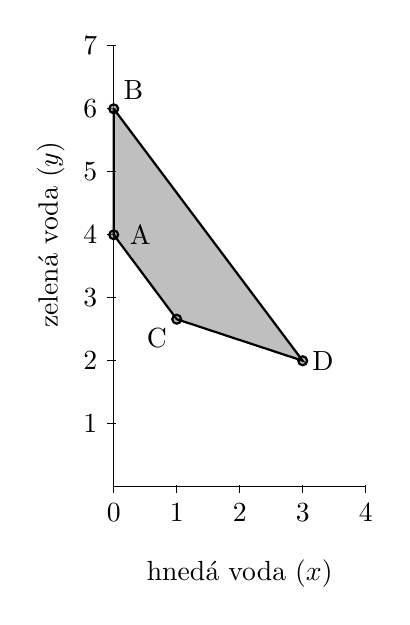
\begin{tikzpicture}[scale=0.8]
  %axis
  \draw (0,0) -- coordinate (x axis mid) (4,0);
  \draw (0,0) -- coordinate (y axis mid) (0,7);
  %ticks
  \foreach \x in {0,...,4}
      \draw (\x,1pt) -- (\x,-3pt);
  \foreach \x in {0,...,4}
      \draw (\x,-3pt) node[anchor=north] {\x};
  \foreach \y in {1,...,7}
      \draw (1pt,\y) -- (-3pt,\y) 
          node[anchor=east] {\y}; 
  %labels      
  \node[below=0.8cm] at (x axis mid) {hnedá voda ($x$)};
  \node[rotate=90] at (-1,4) {zelená voda ($y$)};
  
  \filldraw[fill=black!50, line width=0.8pt, fill opacity=0.5 ]
    (0,6) -- (0,4) -- (1,2.66) -- (3,2) -- (0,6)
    (0,6) circle (2pt)
    (0,4) circle (2pt)
    (1,2.66) circle (2pt)
    (3,2) circle (2pt);

    \draw (0,6) node[anchor=south west]{B};  
    \draw (.1,4) node[anchor=west]{A};  
    \draw (3,2) node[anchor=west]{D};  
    \draw (1,2.66) node[anchor=north east]{C};  
\end{tikzpicture}
\end{minipage}

}

\vskip 2ex
\noindent Riešenia systému $A\bm{x}=\bm{b}$ tvoria rovinu v 5-rozmernom
priestore. Premenné $x,y$ zodpovedajú množstvu kúpenej hnedej a zelenej vody,
premenné $s_1,s_2,s_3$ udávajú rezervu, ktorá ostáva k prekročeniu príslušného
obmedzenia. Takže napríklad štvrtý riadok tabuľky s obmedzeniami $x=s_3=0$
hovorí, že ak študent nekupuje žiadnu hnedú vodu a zároveň chce presne
dosiahnuť povolené množstvo aspartámu, musí kúpiť 6~dl zelenej vody, pričom
dostane viac kofeínu a cukru ako potrebuje. V poslednom riadku vidno, že
obmedzenia sa nedajú pridávať ľubovoľne, ale treba dávať pozor, aby pridaním
obmedzení nevznikli lineárne závislé riadky (v našom prípade sú červená a
fialová priamka z prvého obrázka rovnobežné, takže neexistuje žiaden bod v ich
priesečníku). V reči lineárnych programov sa riadkom tejto tabuľky hovorí {\em
bázové riešenia} a tie z nich, ktoré sú zároveň prípustné (zvýraznené riadky)
sú {\em prípustné bázové riešenia} a zodpovedajú vrcholom \dom, t.j. prípustné
riešenia programu (\ref{eq:LP:2}) tvoria dvojrozmerný štvoruholník v päťrozmernom
priestore.

\noindent
Za povšimnutie stojí, že prípustné bázové riešenia programu
(\ref{eq:LP:2}), t.j. vrcholy štvoruholníka prípustných riešení
v päťrozmernom priestore,  zodpovedajú vrcholom štvoruholníka prípustných riešení 
programu (\ref{eq:LP:1}): každý vrchol štvoruholníka vpravo leží na priesečníku dvoch priamok,
z ktorých každá zodpovedá obmedzeniu tvaru $x_i=0$ (a príslušné bázové riešenie
je prípustné). Naopak, každé prípustné bázové riešenie leží na priesečníku dvoch takýchto priamok.

\vskip 1ex
\noindent
Keď si uvedomíme,
že pridaním obmedzenia tvaru $x=0$ vlastne pri riešení príslušného systému
vymažeme stĺpec premennej $x$ z matice dostaneme nasledovnú definíciu.

\begin{ozn}
Majme maticu $A\in\R^{m\times n}$ s $m$ riadkami a $n$ stĺpcami. Pre množinu
$B\subseteq\{1,2,\ldots,n\}$ označíme $A_B$ podmaticu $A$, ktorá pozostáva zo
stĺpcov indexovaných množinou $B$. Rovnakú notáciu $\bm{x}_B$ budeme používať
pre vektory.
\end{ozn}

\noindent
Napríklad
\begin{align*}
A&=\left(\begin{array}{ccccc}-30&-90&1&0&0\\-40&-30&0&1&0\\30&40&0&0&1\end{array}\right)
 &A_{\{1,2\}}&=\left(\begin{array}{ccccc}-30&-90\\-40&-30\\30&40\end{array}\right)
 &A_{\{3,4,5\}}&=\left(\begin{array}{ccccc}1&0&0\\0&1&0\\0&0&1\end{array}\right)
\end{align*}


\begin{framed} 
  \begin{dfn} 
    \label{dfn:LP:basis} 
    Majme lineárny program v normálnom tvare, kde $A\in\R^{m\times n}$.
    {\bfseries Bázové riešenie} je vektor  $\bm{x}\in\R^n$, pre ktorý existuje
    $m$-prvková množina $B\subseteq\{1,\ldots,n\}$ taká, že
    \begin{enumerate}
      \item matica $A_B\in\R^{m\times m}$ má hodnosť $m$ (t.j. je regulárna)
      \item $x_j=0$ pre všetky $j\not\in B$
    \end{enumerate}
  \end{dfn}
\end{framed}

\noindent Teraz ukážeme, že naša predstava bázového riešenia ako vrchola je dobrá
v tom, že na nájdenie optima stačí overiť prípustné bázové riešenia.

\begin{veta}
Majme daný lineárny program v normálnom tvare, pričom hodnota
účelovej funkcie je $\bm{c}\tr\bm{x}$ na telese \dom je zhora ohraničená.
Potom pre každé prípustné riešenie $\bm{x_0}$ existuje prípustné bázové
riešenie $\bm{\tilde{x}}$, pre ktoré
$\bm{c}\tr\bm{\tilde{x}}\ge\bm{c}\tr\bm{x_0}$.
\end{veta}

\begin{dokaz}
Zoberme si ľubovoľné prípustné riešenie $\bm{x_0}$ a uvažujme všetky také
prípustné riešenia $\bm{x}$, pre ktoré $\bm{c}\tr\bm{x}\ge\bm{c}\tr\bm{x_0}$.
Za $\bm{\tilde{x}}$ vyberme také z nich, ktoré má najväčší počet nulových
zložiek.  Ukážeme, že $\bm{\tilde{x}}$ je bázové.  Ak $\bm{\tilde{x}}=\bm{0}$,
je zrejme bázové. Nech teda $\bm{\tilde{x}}$ má aspoň jednu nenulovú zložku.
Označme $K=\left\{j\in\{1,\ldots,n\}\mid\tilde{x}_j>0\right\}$ množinu kladných
(žiadne prípustné riešenie nemá záporné zložky) zložiek vektora
$\bm{\tilde{x}}$ a uvažujme dva prípady.

\bulpar {\em Stĺpce matice $A_K$ sú lineárne nezávislé.} Zjavne $|K|\le m$
(matica $A$ má $m$ riadkov). Ak $|K|=m$, $\bm{\tilde{x}}$ v zhode s
Definíciou~\ref{dfn:LP:basis} má $\tilde{x_j}=0$ pre všetky $j\not\in K$ a
matica $A_K$ je regulárna. Ak $|K|<m$, môžeme $|K|$ stĺpcov matice $A_K$
doplniť $m-k$ stĺpcami z $A$ tak, aby boli lineárne nezávislé\footnote{Toto
tvrdenie je súčasťou základného kurzu algebry.}.  Takže dostaneme množinu $K'$
tak, že $|K'|=m$, $A_{K'}$ je regulárna a   $\tilde{x_j}=0$ pre všetky
$j\not\in K'\supseteq K$.

\bulpar {\em Stĺpce matice $A_K$ sú lineárne závislé,} to znamená, že existuje
vektor $\bm{\vartheta}\in\R^{|K|}$ taký, že $A_K\bm{\vartheta}=\bm{0}$
(\bm{\vartheta} určuje lineárnu kombináciu stĺpcov $A_K$, ktorej výsledkom je
nulový vektor).  Doplňme \bm{\vartheta} na $n$-rozmerný vektor \bm{w} tak, že
na miesta mimo množiny $K$ dosadíme 0, takže $\bm{w}_K=\bm{\vartheta}$ a
$A\bm{w}=0$.  Pre ľubovoľné reálne $t\ge0$ označme
$\bm{x}(t)=\bm{\tilde{x}}+t\bm{w}$.  Keďže $\bm{\tilde{x}}$ je prípustné
riešenie, platí $A\bm{\tilde{x}}=\bm{b}$. Zároveň platí $A\bm{w}=\bm{0}$ a teda
aj $A\bm{x}(t)=\bm{b}$.

Prv, než budeme pokračovať v dôkaze, upravíme vektor \bm{w} tak, aby
$\bm{c}\tr\bm{w}\ge0$ a zároveň $w_j<0$ pre nejaké $j\in K$.  Ak
$\bm{c}\tr\bm{w}=0$ a pre všetky $j\in K$ platí  $w_j>0$, stačí \bm{w}
prenásobiť -1 a máme ho v požadovanom tvare. Nech teda $\bm{c}\tr\bm{w}\not=0$.
Ak  $\bm{c}\tr\bm{w}<0$, môžme opäť \bm{w} prenásobiť -1, takže bez ujmy na
všeobecnosti nech $\bm{c}\tr\bm{w}>0$. Ukážeme, že teraz musí také existovať
$j\in K$, že $w_j<0$. Ak by to tak nebolo, t.j. ak pre všetky $j\in K$ je
$w_j>0$, zjavne $\bm{w}\ge\bm{0}$ (zložky $i\not\in K$ sme doplnili nulami).
Potom ale $\bm{x}(t)=\bm{\tilde{x}}+t\bm{w}\ge0$ pre všetky $t\ge0$, takže
$\bm{x}(t)$ je prípustné riešenie. Hodnota účelovej funkcie je
$\bm{c}\tr\bm{x}(t)=\bm{c}\tr\bm{\tilde{x}}+t\bm{c}\tr\bm{w}$. Keďže
$\bm{c}\tr\bm{w}>0$, pre $t\mapsto\infty$ je $\bm{c}\tr\bm{x}(t)\mapsto\infty$,
a teda lineárny program nebol ohraničený.

\noindent
Majme teraz vektor \bm{w} upravený tak, že spĺňa  $\bm{c}\tr\bm{w}\ge0$ a
zároveň $w_j<0$ pre nejaké $j\in K$.  Ukážeme, že pre nejaké $t_1>0$ je vektor
$\bm{x}(t_1)$ prípustné riešenie s viacerými nulovými zložkami ako
$\bm{\tilde{x}}$.  To bude ale v spore s tým, že  $\bm{\tilde{x}}$ má najviac
nulových zložiek spomedzi všetkých prípustných riešení $\bm{x}$, pre ktoré
$\bm{c}\tr\bm{x}\ge\bm{c}\tr\bm{x_0}$, pretože
$\bm{c}\tr\bm{x}(t_1)=\bm{c}\tr\bm{\tilde{x}}+t_1\bm{c}\tr\bm{w}\ge\bm{c}\tr\bm{x_0}$
(lebo $\bm{c}\tr\bm{\tilde{x}}\ge\bm{c}\tr\bm{x_0}$ a $\bm{c}\tr\bm{w}\ge0$).

Vektor $\bm{x}(t_0)=\bm{\tilde{x}}$ je prípustné riešenie a má zložky $j\in K$ (ostro) kladné
a zvyšné zložky nulové. Zároveň vieme, že existuje aspoň jedno $j\in K$, kde $w_j<0$.
Keďže $j$-ta zložka $\bm{x}(t)$ je $x(t)_j=\tilde{x}_j+tw_j$, s rastúcim $t$ klesajú hodnoty $x(t)_j$
pre všetky $j$, kde $w_j<0$. Zvoľme za $t_1$ také $t$, keď prvá z hodnôt $x(t)_j$ dosiahne 0.
Zjavne $\bm{x}(t_1)$ je prípustné riešenie a má viac nulových zložiek ako $\bm{\tilde{x}}$.
\end{dokaz}

\noindent Dôsledkom tejto vety je, že na nájdenie optimálneho riešenia pre
lineárne programy, ktoré majú konečné optimum, stačí prehľadať všetky prípustné
bázové riešenia.  Toto prehľadávanie je zovšeobecnením prístupu v dvoch
rozmeroch z úvodného príkladu, kde stačilo prehľadať vrcholy vhodného
mnohouholníka.  Ako sa dajú bázové riešenia nájsť? Stačí si uvedomiť, že pre
danú množinu $B\subseteq\{1,\ldots,n\}$ existuje najviac jedno bázové
riešenie\footnote{Naopak to neplatí, to isté bázové riešenie \bm{x} je možné
  dostať z rôznych množín $B$, $B'$. Ak napríklad vektor \bm{0} je prípustné
riešenie, potom je aj prípustné bázové riešenie pre ľubovoľnú množinu $B$.}:
ak by boli dve bázové riešenia $\bm{y},\bm{z}$ s tou istou množinou $B$, musí
platiť $A\bm{y}=A\bm{z}=\bm{b}$ a teda $A_B\bm{y}=A_B\bm{z}=\bm{b}$. Keďže $A$
je regulárna štvorcová matica, systém $A_B\bm{x}=\bm{b}$ má jednoznačné riešenie
a preto $\bm{y}=\bm{z}$.
Preto stačí vyskúšať všetky množiny $B$, overiť, či príslušná $A_B$ je regulárna (napr. Gaussovou elimináciou),
overiť, či je získané riešenie $A_B\bm{x}=\bm{b}$ prípustné a spomedzi všetkých takto získaných riešení
\bm{x} vybrať to najlepšie.
Problém s týmto algoritmom je, že pri $n$ premenných a $m$
obmedzeniach môže byť potenciálne ${n\choose m}$ rôznych bázových riešení, a
teda vo všeobecnosti nie je polynomiálny\footnote{%
  Napríklad pre $m=n/2$ sa zo Stirlingovej aproximácie $n!\approx\sqrt{2\pi n}\left(\frac{n}{e}\right)^n\left(1+o(n)\right)$ ľahko
ukáže, že \hbox{$\left(n\atop \frac{n}{2}\right)=\frac{n!}{\left[\left(\frac{n}{2}\right)!\right]^2}\ge 2^n/n^2$.}}.
V nasledujúcej časti si ukážeme, ako úlohu lineárneho programovania riešiť efektívnejšie
pomocou simplexovej metódy.



% % % % % % % % % % % % % % % % % % % % % % % % % % % % % % % % % % % % % % % %
\section{Simplexová metóda}
\renewcommand{\common}{
      \draw[dashed]
        (0,0,0) -- (6,0,0)
        (0,0,0) -- (0,4,0)
        (0,0,0) -- (0,0,4);
    
    \draw
      (1,0,4) -- (5,4,0) -- (0,3,3) -- (0,1,4) -- (1,0,4) -- (0,0,4) -- (0,1,4)
      (1,0,4) -- (6,0,0) -- (5,4,0) -- (0,4,0) -- (0,3,3);


}

\newcommand{\tmpSimplexNode}[2]{
  (#1) circle (1.2pt) node[anchor=#2] {\footnotesize $(#1)$}
}

\noindent
Ako simplexový algoritmus sa označuje každý taký greedy algoritmus, ktorý 
prechádza bázové riešenia (vrcholy \dom) tak, že vždy sa presunie po hrane smerom, v ktorom
rastie (pri maximalizácii) hodnota účelovej funkcie. 
Začnime opäť príkladom. Uvažujme nasledovný lineárny program:

\begin{equation}
  \label{simplex:eq:1}
  \begin{array}{rllll}
    \text{maximalizovať}& x & +\;y & +\;z & =:  f(x,y,z)\\
  \text{pri obmedzeniach}& x & +\;y & +\;2z & \le 9\\
                         & 4x & +\;y&+\;5z&\le 24\\
                         &    &\phantom{+}\;3y&+\;z&\le 12\\
                         &    &     &\phantom{+}\;z&\le 4\\
\multicolumn{4}{r}{x,y,z}&\ge 0
 

  \end{array}
\end{equation}


\begin{minipage}[t]{0.4\textwidth}
  \vskip 0pt
\noindent
Obmedzenia tvoria polpriestory v trojrozmernom priestore. 
Hraničné roviny (v poradí zelená, modrá, červená a žltá)
vymedzujú mnohosten \dom.
Preskúšaním všetkých vrcholov \dom zistíme, že maximum
sa dosahuje v bode $(5,4,0)$. 
\end{minipage}\hfill
\begin{minipage}[t]{0.6\textwidth}
  \vskip 0pt

\begin{center}
  \tdplotsetmaincoords{70}{120}
  \begin{tikzpicture}[scale=0.62,tdplot_main_coords]

    \fill[fill=blue!20]
      (6,0,0) -- (5,4,0) -- (1,0,4);
    \fill[fill=green!20]
      (5,4,0) -- (0,3,3) -- (0,1,4) -- (1,0,4); 
    \fill[fill=magenta!20]
      (5,4,0) -- (0,4,0) -- (0,3,3); 
    \fill[fill=yellow!20]
      (0,0,4) -- (0,1,4) -- (1,0,4); 

    \draw[->,thin]
      (6,0,0) -- (7,0,0) node[anchor=north east]{$x$};
    \draw[->,thin]
      (0,4,0) -- (0,5,0) node[anchor=north west]{$y$};
    \draw[->,thin]
      (0,0,4) -- (0,0,5) node[anchor=south]{$z$};

    \common
    \filldraw
    \tmpSimplexNode{0,0,4}{south west}
    \tmpSimplexNode{1,0,4}{east}
    \tmpSimplexNode{0,3,3}{west}
    \tmpSimplexNode{0,4,0}{south west}
    \tmpSimplexNode{5,4,0}{north west}
    \tmpSimplexNode{6,0,0}{south east}
    \tmpSimplexNode{0,1,4}{west};
    
  \end{tikzpicture}
  \end{center}
\end{minipage}

\noindent 
Podobne ako v predchádzajúcej časti si zavedieme rezervné ({\em
slack}) premenné $s_1,\ldots,s_4$;  ak si premenné očíslujeme v poradí $x,y,z,s_1,\ldots,s_4$,
dostaneme ekvivalentný program 
v normálnom tvare

$$\max_{\bm{x}\in\R^7}\left\{ \bm{c}\tr\bm{x} \mid A\bm{x}=\bm{b},\; \bm{x}\ge0
\right\}$$ 
%
kde
\begin{align*}
 \bm{c}&=\cvect{1\\1\\1\\0\\0\\0\\0}
&A&=\left(\begin{array}{ccccccc}
  1&1&2&1&0&0&0\\
  4&1&5&0&1&0&0\\
  0&3&1&0&0&1&0\\
  0&0&1&0&0&0&1
\end{array}\right)
&\bm{b}&=\cvect{9\\24\\12\\4}
\end{align*}

\noindent
Máme 7 premenných a matica $A$ má hodnosť 4, teda riešenia systému $A\bm{x}=\bm{b}$ tvoria trojrozmerný
podpriestor v sedemrozmernom priestore. Špeciálne, môžme si vybrať ľubovoľné tri premenné ako parametre
a ostatné premenné (aj hodnotu funkcie) vyjadriť pomocou nich. V našom prípade je matica $A_{4,5,6,7}$
diagonálna, takže ľahko vidno, že program (\ref{simplex:eq:1}) je ekvivalentne zapísateľný takto:

\vskip 2ex
\begin{minipage}[c]{7cm}
  \vskip 0pt
\begin{equation}
  \label{simplex:eq:2}
  \begin{array}{r<{ = }llll}
    f  &    &  \phantom{+}\;x  & +\;y   &+\;z\\[1ex]\hline\rule{0mm}{3ex}
   s_1 & 9  &  -\;x            & -\;y   & -\;2z \\
   s_2 & 24 &  -\;4x           & -\;y   & -\;5z \\
   s_3 & 12 &                  & -\;3y  & -\;z\\
   s_4 & 4  &                  &        & -\;z 
  \end{array}
\end{equation}
\end{minipage}\hfill\begin{minipage}[c]{4cm}
  \vskip 0pt
  \tdplotsetmaincoords{70}{120}
  \begin{tikzpicture}[scale=0.4,tdplot_main_coords]
  \common
    %\filldraw
    %\tmpSimplexNode{0,0,0}{east} ;
    \fill[color=red]
      (0,0,0) circle (5pt);
  \end{tikzpicture}
\end{minipage}
\vskip 3ex

\noindent
Zápisu (\ref{simplex:eq:2}) budeme hovoriť {\em tablo} a znamená toto: hľadáme parametre $x,y,z$ tak,
aby hodnota $f$ bola maximálna a pritom parametre $s_1,\ldots,s_4$ boli nezáporné. V našom prípade
vidno, že pri voľbe $x=y=z=0$ bude nezápornosť $s_1,\ldots,s_4$ splnená. Tablo (\ref{simplex:eq:2})
preto bude reprezentovať bázové riešenie $(0,0,0,9,24,12,4)$ pre bázu $\{s_1,s_2,s_3,s_4\}$ s hodnotou funkcie $f=0$.
Bázové premenné sú v riadkoch a nebázové nulové premenné sú parametre v stĺpcoch.

\noindent
Obrázok vpravo graficky reprezentuje bázové riešenie z tabla (\ref{simplex:eq:2}). 
Čitateľa môže miasť, že na obrázku je trojrozmerné teleso, hoci náš program má 7 rozmerov. 
Problém je v tom, že obrázky zo sedemrozmerného priestoru sa do textu veľmi zle vkladajú. Vizualizáciu preto 
budeme robiť v pôvodnom trojrozmernom priestore z príkladu (\ref{simplex:eq:1}). Konkrétne, ak  
riešeniu $(x,y,z,s_1,s_2,s_3,s_4)$ priradíme bod $(x,y,z)$, hodnoty $(s_1,s_2,s_3,s_4)$ sa dajú dopočítať ako
vzdialenosti od príslušných stien (pretože matica $A$ má hodnosť 4, máme vždy 3 voľné parametre a vrcholy mnohostena 
vpravo zodpovedajú bázovým riešeniam).

\noindent
Naším cieľom je nájsť najlepšie prípustné bázové riešenie, resp. jeho bázu.
Chceme teda nájsť nejaké tri nebázové premenné (parametre),
ktoré sa nastavia na 0 a z vyjadrenia ostatných premenných (a účelovej funkcie) pomocou
týchto parametrov vieme určiť ich hodnoty. Vyskúšanie všetkých trojíc parametrov
by preto zodpovedalo prehľadaniu všetkých bázových riešení (vrcholov mnohostenu). Tomuto sa ale
snažíme vyhnúť.

\noindent
Ako môžme lokálne zväčšiť hodnotu funkcie $f$? Vidíme, že napr. premenná $z$ je v prvom riadku s kladným koeficientom,
takže ak zvýšime hodnotu $z$, vzrastie aj $f$. Ako veľa môžme $z$ zväčšiť? Všetky premenné $s_1,\ldots,s_4$
musia zostať nezáporné, takže každý riadok nám dáva limit na maximálnu hodnotu $z$ v poradí
$\frac{9}{2}$, $\frac{24}{5}$, $12$, $4$. 
Môžme teda nastaviť $z=4$, čím dostaneme, že $s_4=0$. Naše riešenie sa teda zmenilo tak, že nebázové premenné
(parametre) budú $x,y,s_4$ namiesto $x,y,z$. Prispôsobíme tomu aj náš zápis tak, že z rovnice pre $s_4$ vyjadríme 
$z$ a dosadíme do ostatných rovníc. Dostaneme tak zápis

\vskip 2ex
\begin{minipage}[c]{7cm}
  \vskip 0pt
\begin{equation}
  \label{simplex:eq:3}
  \begin{array}{r<{ = }llll}
    f  & 4  &  +\;x  & +\;y   &-\;s_4\\[1ex]\hline\rule{0mm}{3ex}
   z   & 4  &        &        & -\;s_4 \\
   s_1 & 1  &  -\;x  & -\;y   & +\;2s_4 \\
   s_2 & 4  &  -\;4x & -\;y   & +\;5s_4 \\
   s_3 & 8  &        & -\;3y  & +\;s_4
  \end{array}
\end{equation}
\end{minipage}\hfill\begin{minipage}[c]{4cm}
  \vskip 0pt
  \tdplotsetmaincoords{70}{120}
  \begin{tikzpicture}[scale=0.4,tdplot_main_coords]
  \common
    \filldraw
      \tmpSimplexNode{0,0,4}{south west} ;
    \filldraw[color=red]
      (0,0,0) circle (4pt)
      (0,0,4) circle (5pt);
    \draw[very thick,dashed,color=red] 
      (0,0,0) -- (0,0,4);
  \end{tikzpicture}
\end{minipage}
\vskip 3ex

\noindent
Tablo (\ref{simplex:eq:3}) zodpovedá bázovému riešeniu $(0,0,4,1,4,8,0)$ pre bázu $\{z,s_1,s_2,s_3\}$
s hodnotou funkcie $f=4$. Opäť máme zápis, kde v riadkoch sú bázové premenné a parametre stĺpcov sú
nebázové premenné. Cieľom je nájsť parametre $x,y,s_4$ tak aby sa maximalizovala hodnota $f$ a zároveň
$s_1,s_2,s_3,z$ ostali nezáporné. Je kľúčové si uvedomiť, že sme urobili iba ekvivalentnú úpravu systému
lineárnych rovníc a teda riešenia (\ref{simplex:eq:2}) a (\ref{simplex:eq:3}) sú rovnaké. Krok
z  (\ref{simplex:eq:2}) do (\ref{simplex:eq:3}) zodpovedá prejdeniu po jednej hrane mnohostena riešení.
Budeme ho volať {\em pivotný krok}: jedna nebázová premenná, {\em pivot}, v našom prípade $z$, sa presunula
do bázy a jedna bázová premenná (v našom prípade $s_4$) sa stala nebázovou. Tento postup môžme opakovať.
Vidíme napr., že $y$ je v prvom riadku s kladným koeficientom a teda jeho zväčšením zväčšíme $f$. Jednotlivé
riadky nám dávajú obmedzenia na maximálnu hodnotu $y$ v poradí $1,4,\frac{8}{3}$; v poslednej rovnosti
$y$ nevystupuje a preto naň nekladie ani žiadne obmedzenia. Zvolíme $y=1$ a urobíme pivotný krok s pivotom 
$y$, pri ktorom $y$ vystrieda v báze $s_1$. Vyjadríme $y=1-x-s_1+2s_4$ a po dosadení dostaneme

\vskip 2ex
\begin{minipage}[c]{7cm}
  \vskip 0pt
\begin{equation}
  \label{simplex:eq:4}
  \begin{array}{r<{ = }llll}
    f  & 5  &        & -\;s_1 &+\;s_4\\[1ex]\hline\rule{0mm}{3ex}
    y  & 1  &  -\;x  & -\;s_1 &+\;2s_4\\ 
    z  & 4  &        &        & -\;s_4 \\
   s_2 & 3  &  -\;3x & +\;s_1 & +\;3s_4 \\
   s_3 & 5  &  +\;3x & +\;3s_1& -\;5s_4
  \end{array}
\end{equation}
\end{minipage}\hfill\begin{minipage}[c]{4cm}
  \vskip 0pt
  \tdplotsetmaincoords{70}{120}
  \begin{tikzpicture}[scale=0.4,tdplot_main_coords]
  \common
    \filldraw
      \tmpSimplexNode{0,1,4}{west} ;
    \filldraw[color=red]
      (0,0,0) circle (4pt)
      (0,1,4) circle (5pt)
      (0,0,4) circle (4pt);
    \draw[very thick,dashed,color=red] 
      (0,0,0) -- (0,0,4);
    \draw[very thick,color=red] 
      (0,0,4) -- (0,1,4);
  \end{tikzpicture}
\end{minipage}
\vskip 3ex

\noindent
Máme tablo pre bázové riešenie $(0,1,4,0,3,5,0)$ pre bázu $\{y,z,s_2,s_3\}$ s hodnotou funkcie $f=5$.
Pokračujeme ďalej;  jediná možnosť, ako zvýšiť $f$ je zvoliť pivota $s_4$ a nahradiť ním v báze $s_3$.
Dostaneme

\vskip 2ex
\begin{minipage}[c]{7cm}
  \vskip 0pt
\begin{equation}
  \label{simplex:eq:5}
  \begin{array}{r<{ = }llll}
    f  & 6  &  +\;\frac{3}{5}x      & -\;\frac{2}{5}s_1 &-\;\frac{1}{5}s_3\\[1ex]\hline\rule{0mm}{3ex}
    y  & 3  &  +\;\frac{1}{5}x  & +\;\frac{1}{5}s_1 &-\;\frac{2}{5}s_3\\[1ex] 
    z  & 3  &  -\;\frac{3}{5}x  &  -\frac{3}{5}s_1      & +\;\frac{1}{5}s_3 \\[1ex]
   s_2 & 6  &  -\;\frac{6}{5}x & +\;\frac{14}{5}s_1 & -\;\frac{3}{5}s_3 \\[1ex]
   s_4 & 1  &  +\;\frac{3}{5}x & +\;\frac{3}{5}s_1& -\;\frac{1}{5}s_3
  \end{array}
\end{equation}
\end{minipage}\hfill\begin{minipage}[c]{4cm}
  \vskip 0pt
  \tdplotsetmaincoords{70}{120}
  \begin{tikzpicture}[scale=0.4,tdplot_main_coords]
  \common
    \filldraw
      \tmpSimplexNode{0,3,3}{south west} ;
    \filldraw[color=red]
      (0,0,0) circle (4pt)
      (0,1,4) circle (4pt)
      (0,3,3) circle (5pt)
      (0,0,4) circle (4pt);
    \draw[very thick,dashed,color=red] 
      (0,0,0) -- (0,0,4);
    \draw[very thick,color=red] 
      (0,0,4) -- (0,1,4) -- (0,3,3);
  \end{tikzpicture}
\end{minipage}
\vskip 3ex

\noindent
Opäť jediná možnosť, ako spraviť pivotný krok, je zobrať do bázy $x$. Pri nastavení $x=5$ sa ale vynulujú
$z$ aj $s_2$ a môžme si vybrať, ktoré z nich v báze ponecháme. Nech $x$ vystrieda v báze $z$, dostaneme

\vskip 2ex
\begin{minipage}[c]{7cm}
  \vskip 0pt
\begin{equation}
  \label{simplex:eq:6}
  \begin{array}{r<{ = }llll}
    f  & 9  &   -\;z     & -\;s_1 &\\[1ex]\hline\rule{0mm}{3ex}
    x  & 5  &  -\;\frac{5}{3}z & -\;s_1 & +\;\frac{1}{3}s_3\\[1ex]
    y  & 4  &  -\;\frac{1}{3}z  & &-\;\frac{1}{3}s_3\\[1ex] 
   s_2 &   & \phantom{-}\;2z & +\;4s_1 & -\;s_3 \\
   s_4 & 4  & -\;z  & &
  \end{array}
\end{equation}
\end{minipage}\hfill\begin{minipage}[c]{4cm}
  \vskip 0pt
  \tdplotsetmaincoords{70}{120}
  \begin{tikzpicture}[scale=0.4,tdplot_main_coords]
  \common
    \filldraw
      \tmpSimplexNode{5,4,0}{north west} ;
    \filldraw[color=red]
      (0,0,0) circle (4pt)
      (0,1,4) circle (4pt)
      (0,3,3) circle (4pt)
      (5,4,0) circle (5pt)
      (0,0,4) circle (4pt);
    \draw[very thick,dashed,color=red] 
      (0,0,0) -- (0,0,4);
    \draw[very thick,color=red] 
      (0,0,4) -- (0,1,4) -- (0,3,3) -- (5,4,0);
  \end{tikzpicture}
\end{minipage}
\vskip 3ex

\noindent
Dostali sme sa do situácie, keď nie je možné urobiť žiaden pivotný krok. Vieme ale, že
sme robili iba ekvivalentné úpravy, a teda riešenia programov (\ref{simplex:eq:1}) a (\ref{simplex:eq:6})
sú rovnaké (programy majú rovnakú množinu prípustných riešení a rovnaké hodnoty účelovej funkcie).
Lenže z (\ref{simplex:eq:6}) jasne vidno, že pre ľubovoľné nezáporné $z$ a $s_1$, hodnota $f$ je
vždy nanajvýš $9$, takže nájdené riešenie je optimálne.

\vskip 1ex
\noindent
Tento príklad môžme zovšeobecniť. Formálne si tablo prislúchajúce prípustnému bázovému riešeniu môžme
zadefinovať takto:


\begin{framed}
  \begin{dfn}
  \label{dfn:tablo}
Majme program v normálnom tvare
$$\max_{\bm{x}\in\R^n}\left\{ \bm{c}\tr\bm{x} \mid A\bm{x}=\bm{b},\; \bm{x}\ge0
\right\}$$
kde $A\in\R^{m\times n}$, a jeho prípustné bázové riešenie prislúchajúce báze $B$. {\bfseries Tablo} $\T(B)$
prislúchajúce báze $B$ je systém $m+1$ lineárnych rovníc v premenných $x_1,\ldots,x_n,f$,
ktorý má rovnakú množinu riešení ako systém $ A\bm{x}=\bm{b}, f= \bm{c}\tr\bm{x}$
a v maticovom zápise vyzerá
$$
\begin{array}{lllll}
  f & = & f_0 & + & \bm{r}\tr\bm{x}_N\\\hline
  \bm{x}_B & = & \bm{p} & + & Q\;\bm{x}_N
\end{array}
$$
kde $\bm{x}_B$ je vektor bázových premenných, $N=\{1,\ldots,n\}-B$, $\bm{x}_N$ je vektor nebázových
premenných, $\bm{r}\in\R^{n-m}$, $\bm{p}\in\R^m$ a $Q\in\R^{m\times n-m}$.
\end{dfn}
\end{framed}

\noindent
Keďže sme v definícii tabla vychádzali z prípustného bázového riešenia  $B$, zrejme $\bm{p}\ge\bm{0}$.
Ľahko sa presvedčíme, že takáto definícia tabla je korektná. Stačí si uvedomiť, že 
$\bm{b}=A\bm{x}=A_B\bm{x}_B+A_N\bm{x}_N$ a $A_B$ je regulárna, takže existuje inverzná matica
$A_B^{-1}$. Preto platí $\bm{x}_B=A_B^{-1}\bm{b}-A_B^{-1}A_N\bm{x}_N$ a dostávame nasledujúcu lemu,
ktorej podrobný dôkaz prenechávame na čitateľa:

\begin{lema}
  \label{lm:LPtablo}
  Každému prípustnému bázovému riešeniu $B$ programu z definície~\ref{dfn:tablo} prislúcha
  práve jedno tablo $\T(B)$ a platí
  \begin{align*}
    \bm{p} &= A_B^{-1}\bm{b} &
    Q      &= -A_B^{-1}A_N &
    f_0    &= \bm{c}_B\tr A_B^{-1}\bm{b}&
    \bm{r} &= \bm{c}_N-(\bm{c}_B\tr A_B^{-1} A_N)\tr.
  \end{align*}
\end{lema}

\noindent
Z rovnakých úvah, ako sme robili v úvodnom príklade vyplýva

\begin{clm}
  \label{clm:simplexend}
  Nech $B$ je báza prípustného riešenia a nech v $\T(B)$ je $\bm{r}\le\bm{0}$. Potom
  $f_0$ je maximálna hodnota daného programu.
\end{clm}

\noindent
Na to, aby sme dokončili opis simplexového algoritmu, potrebujeme definovať pivotný krok:
vybrať nejakú nebázovú premennú, ktorá je v $\bm{r}\tr\bm{x}_N$ s kladným koeficientom,
zvýšiť ju koľko sa dá tak, aby bázové premenné ostali nezáporné a zmeniť bázu.
Označme si $B=\{\beta_1,\ldots,\beta_m\}$ tak, že $\beta_1<\beta_2<\cdots<\beta_m$
a podobne $N=\{\mu_1,\ldots,\mu_{n-m}\}$, kde $\mu_1<\mu_2<\cdots<\mu_{n-m}$.
V tomto označení môžme tablo rozpísať ako

\begin{equation}
  \label{LP:tablo-ext}
\begin{array}{lllll}
  f & = & f_0 & + & \sum\limits_{j=1}^{n-m} r_jx_{\mu_j}\\[2mm]\hline\rule{0mm}{4ex}
  x_{\beta_1} & = & p_1 & + & \sum\limits_{j=1}^{n-m}q_{1,j}x_{\mu_j}\\
    \vdots    &  & & \vdots\\
  x_{\beta_m} & = & p_m & + & \sum\limits_{j=1}^{n-m}q_{m,j}x_{\mu_j}\\
\end{array}
\end{equation}

\noindent
Za pivota môžme zobrať hocijakú premennú $x_{\mu_j}$ takú, že $r_j>0$. Ak je $q_{i,j}>0$, $i$-ty 
riadok nekladie žiadne obmedzenia, inak musí platiť
$p_i+q_{i,j}x_{\mu_j}>0$.
Dostávame sa tak k nasledovnej definícii:


\begin{framed}
  \begin{dfn}
    \label{dfn:LP:pivot}
    Majme daný lineárny program v normálnom tvare a bázu $B$ prislúchajúcu prípustnému riešeniu. Nech $\T(B)$
    je zapísané ako v (\ref{LP:tablo-ext}) a nech $r_e>0$ pre nejaké $e$.
    Označme $$s:=\min_{i=1,\ldots,m}\left\{-\frac{p_i}{q_{i,e}}\mid q_{i,e}<0\right\}.$$
    {\bfseries Pivotný krok} podľa premennej $x_{\mu_e}$ zmení bázu $B$ na bázu 
    $$B':=\left(B-\{\beta_\ell\}\right)\cup\{\mu_e\},$$
    kde $\beta_\ell$ je ľubovoľný index, pre ktorý  platí
    $q_{\ell,e}<0$ a 
      $-\frac{p_\ell}{q_{\ell,e}} =s$.
  \end{dfn}
\end{framed}


\noindent
Čitateľ sa ľahko presvedčí, že $B'$ je opäť báza prípustného riešenia.
Simplexový algoritmus začína z nejakého prípustného riešenia s bázou $B_0$ a aplikuje pivotné kroky, kým sa dá.
Podľa tvrdenia~\ref{clm:simplexend}, ak algoritmus nájde bázu $B$, pre ktorú je $\bm{r}\le\bm{0}$,
tak našiel optimálne riešenie.
Aby sme ukázali korektnosť simplexovej metódy, potrebujeme vyriešiť tri problémy: jednak ukázať, ako nájsť $B_0$, 
dvak rozhodnúť, čo robiť, keď
sa nedá urobiť žiaden pivotný krok a napokon ukázať, že algoritmus v konečnom čase skončí.

\subsection*{Čo sa stane, keď sa nedá vybrať pivot}

\noindent
Definícia pivotného kroku (Definícia~\ref{dfn:LP:pivot}) vyžaduje, aby pre pivota $x_{\mu_e}$ platilo $r_e>0$.
Ak neexistuje $x_{\mu_e}$, pre ktoré $r_e>0$,
podľa Tvrdenia~\ref{clm:simplexend} máme optimálne riešenie.
Ďalej musí platiť, že
pivot nahradí v báze premennú $x_{\beta_\ell}$, pre ktorú $q_{\ell,e}<0$.
Ak také $\ell$ neexistuje, t.j. ak $q_{\ell,e}\ge0$ pre všetky $\ell$, znamená to,
že žiaden riadok tabla nekladie limit na zväčšovanie premennej $x_{\mu_e}$. S rastúcim $x_{\mu_e}$
rastie aj hodnota $f$, a preto daný program nemá konečné maximum.

\subsection*{Ako sa nezacykliť}

\noindent
V úvodnom príklade sme 
v každom pivotnom kroku zväčšili hodnotu $f$. Ak by sme to vedeli zaručiť vždy, ľahko vidno,
že algoritmus v konečnom čase skončí: je totiž iba konečne veľa bázových riešení.
Čo by sa ale stalo, keby sme sa v kroku (\ref{simplex:eq:5}) rozhodli, že $x$ nevystrieda v báze $z$ ale $s_2$?
Namiesto tabla  (\ref{simplex:eq:6})
dostaneme tablo

\vskip 2ex
\begin{minipage}[c]{7cm}
  \vskip 0pt
\begin{equation}
  \label{simplex:eq:7}
  \begin{array}{r<{ = }llll}
    f  & 9  &   +\;s_1     & -\;\frac{1}{2}s_2 & -\;\frac{1}{2}s_3\\[1ex]\hline\rule{0mm}{3ex}
    x  & 5  &  +\;\frac{7}{3}s_1 & -\;\frac{5}{6}s_2 & -\;\frac{1}{2}s_3\\[1ex]
    y  & 4  &  +\;\frac{2}{3}s_1  & -\;\frac{1}{6}s_2 & -\;\frac{1}{2}s_3\\[1ex] 
    z  &   & -\;2s_1 & +\;\frac{1}{2}s_2 & +\;\frac{1}{2}s_3 \\[1ex]
    s_4 & 4  & +\;2s_1  &  -\;\frac{1}{2}s_2 & -\;\frac{1}{2}s_3
  \end{array}
\end{equation}
\end{minipage}\hfill\begin{minipage}[c]{4cm}
  \vskip 0pt
  \tdplotsetmaincoords{70}{120}
  \begin{tikzpicture}[scale=0.4,tdplot_main_coords]
  \common
    \filldraw
      \tmpSimplexNode{5,4,0}{north west} ;
    \filldraw[color=red]
      (0,0,0) circle (4pt)
      (0,1,4) circle (4pt)
      (0,3,3) circle (4pt)
      (5,4,0) circle (5pt)
      (0,0,4) circle (4pt);
    \draw[very thick,dashed,color=red] 
      (0,0,0) -- (0,0,4);
    \draw[very thick,color=red] 
      (0,0,4) -- (0,1,4) -- (0,3,3) -- (5,4,0);
  \end{tikzpicture}
\end{minipage}
\vskip 3ex

\noindent
Tablo (\ref{simplex:eq:6}) reprezentuje bázu $\{x,y,s_2,s_4\}$ a tablo (\ref{simplex:eq:7})
bázu $\{x,y,z,s_4\}$, pričom obidvom bázam prislúcha rovnaké riešenie
$(5,4,0,0,0,0,4)$. Zo zápisu (\ref{simplex:eq:7}) ale nevidno, že sme už našli optimum,
a preto treba urobiť ešte jeden pivotný krok s pivotom $s_1$. Pri tomto kroku ale zistíme,
že premenná $z$ nedovolí zväčšiť $s_1$, a tak sme nútení urobiť krok ``naprázdno'' 
a vymeniť v báze $s_1$ za $z$. Dostaneme tablo

\vskip 2ex
\begin{minipage}[c]{7cm}
  \vskip 0pt
\begin{equation}
  \label{simplex:eq:8}
  \begin{array}{r<{ = }llll}
    f  & 9  &   -\;\frac{1}{2}z  & -\;\frac{1}{4}s_2 & -\;\frac{1}{4}s_3\\[1ex]\hline\rule{0mm}{3ex}
    x  & 5  &  -\;\frac{7}{6}z & -\;\frac{1}{4}s_2 & +\;\frac{1}{12}s_3\\[1ex]
    y  & 4  &  -\;\frac{1}{3}z  & & -\;\frac{1}{3}s_3\\[1ex] 
    s_1  &   & -\;\frac{1}{2}z & +\;\frac{1}{4}s_2 & +\;\frac{1}{4}s_3 \\[1ex]
    s_4 & 4  & -\;z
  \end{array}
\end{equation}
\end{minipage}\hfill\begin{minipage}[c]{4cm}
  \vskip 0pt
  \tdplotsetmaincoords{70}{120}
  \begin{tikzpicture}[scale=0.4,tdplot_main_coords]
  \common
    \filldraw
      \tmpSimplexNode{5,4,0}{north west} ;
    \filldraw[color=red]
      (0,0,0) circle (4pt)
      (0,1,4) circle (4pt)
      (0,3,3) circle (4pt)
      (5,4,0) circle (5pt)
      (0,0,4) circle (4pt);
    \draw[very thick,dashed,color=red] 
      (0,0,0) -- (0,0,4);
    \draw[very thick,color=red] 
      (0,0,4) -- (0,1,4) -- (0,3,3) -- (5,4,0);
  \end{tikzpicture}
\end{minipage}
\vskip 3ex

\noindent
z ktorého už vidno optimalitu. 
Tento degenerovaný krok ale nezvýšil hodnotu $f$, čím
rozbil náš pôvodný argument o zastavení: nevieme totiž zaručiť, že hodnota $f$ sa v každom
kroku zväčší. Nutnosť spraviť degenerovaný pivotný krok nemusí nastať iba na konci, keď
už máme optimálne riešenie, 
ako ukazuje jednoduchý príklad (podľa \cite{MG07}):

\noindent
\begin{minipage}[t]{6cm}
  \vskip 0pt
\begin{equation*}
  \begin{array}{rlll}
    \text{maximalizovať}&  & y & =:  f(x,y)\\
  \text{pri obmedzeniach}& -\;x & +\;y & \le 0\\
                         & \phantom{-\;}x &  & \le 2\\
\multicolumn{3}{r}{x,y}&\ge 0
  \end{array}
\end{equation*}
\end{minipage}
  \hfill
\begin{minipage}[t]{5cm}
    \vskip 0pt
\begin{tikzpicture}[scale=1.2]

  \filldraw[color=blue!30]
    (0,0) -- (2,0) -- (2,2) -- cycle;

  \halfplane{0,0}{3,0}{+}{0.2cm}{0.8cm}
  \halfplane{0,0}{0,3}{-}{0.2cm}{1cm}
  \halfplane{2,0}{2,3}{+}{0.2cm}{1cm}
  \halfplane{0,0}{2,2}{-}{0.2cm}{2cm}
  \draw 
    (0,3.5) node[anchor=south west]{$x\ge 0$}
    (2,3.5) node[anchor=south west]{$x\le 2$}
    (2.5,1.8) node[anchor=south west]{$x\ge y$}
    (2.5,0.3) node[anchor=south west] {$y\ge 0$};



  %axis
  \draw (-.2,0) -- coordinate (x axis mid) (3,0);
  \draw (0,-.2) -- coordinate (y axis mid) (0,3);
  %ticks
  \foreach \x in {-0,...,2}
      \draw (\x,1pt) -- (\x,-3pt);
  \foreach \x in {0,...,2}
      \draw (\x,-3pt) node[anchor=north] {\x};
  \foreach \y in {1,...,2}
      \draw (1pt,\y) -- (-3pt,\y)
          node[anchor=east] {\y};

\end{tikzpicture}
\end{minipage}

\noindent
Keď zavedieme rezervné premenné $s_1, s_2$, dostaneme tablo

$$
  \begin{array}{r<{ = }lll}
    f    &    &     & \phantom{-\;}y \\[1ex]\hline\rule{0mm}{3ex}
    s_1  &    & \phantom{-\;}x   & -y \\
    s_2  & 2  & -\;x
  \end{array}
$$

\noindent
pre bázu $\{s_1,s_2\}$ s hodnotou riešenia $f=0$. Jediná možnosť, ako pokračovať (a dostať sa 
k optimálnemu riešeniu s hodnotou $2$), je spraviť degenerovaný pivotný krok, v ktorom $y$ vystrieda v báze 
$s_1$:
$$
  \begin{array}{r<{ = }lll}
    f    &    &  \phantom{-\;}x   & -\;s_1 \\[1ex]\hline\rule{0mm}{3ex}
    y    &    & \phantom{-\;}x   & -s_1 \\
    s_2  & 2  & -\;x
  \end{array}
$$

\noindent
Podobná situácia je sa vyskytuje pomerne často. 

\begin{framed}
  \begin{dfn}
    {\em Degenerovaný krok} simplexového algoritmu je taký pivotný krok, pri ktorom sa báza $B$ 
    transformuje na bázu $B'$ s rovnakým bázovým riešením.
  \end{dfn}
\end{framed}


\noindent
Degenerovaným krokom sa nevieme vyhnúť a navyše
nasledovný príklad z \cite{Ch83} ukazuje, že ak nie sme dosť opatrní, môžme sa zacykliť.
Uvažujme nasledovné tablo:

\begin{equation}
  \begin{array}{r<{ = }lllll}
    f    &    & \phantom{-\;} 10x_1    & -\;57x_2   &  -\;9x_3   &  -\;24x_4  \\[1ex]\hline\rule{0mm}{3ex}
    x_5  &    & -\;0.5x_1 & +\;5.5x_2  &  +\;2.5x_3 &  -\;9x_4\\
    x_6  &    & -\;0.5x_1 & +\;1.5x_2  &  +\;0.5x_3 &  -\;x_4\\
    x_7  &  1 & -\;x_1
  \end{array}
\end{equation}

\noindent
pre bázu $\{x_5,x_6,x_7\}$.
Predpokladajme, že konkrétny simplexový algoritmus vždy vyberie ako pivota nebázovú premennú $x_{\mu_e}$ s maximálnou
hodnotou $r_e$. V prípade, že pivotný krok vynuluje viacero bázových premenných, vyberie sa premenná s minimálnym indexom.
Nechávame ako cvičenie pre čitateľa overiť, že algoritmus v nasledujúcich iteráciách prejde cez bázy
$\{x_1,x_6,x_7\}$, $\{x_1,x_2,x_7\}$, $\{x_2,x_3,x_7\}$, $\{x_3,x_4,x_7\}$, $\{x_4,x_5,x_7\}$ a napokon sa dostane 
naspäť do $\{x_5,x_6,x_7\}$. Keďže vznikol cyklus z degenerovaných pivotných krokov, algoritmus sa zacyklí.

\noindent
Vidíme, že nemôžeme dúfať, že dokážeme termináciu simplexovej metódy pre ľubovoľnú voľbu pivota, ale musíme zafixovať
nejaký konkrétny algoritmus pre pivotný krok. 
Existuje veľa alternatívnych pravidiel
na výber pivota, s rôznymi prístupmi k problému zacyklenia. My na dôkaz terminácie použijeme {\em pravidlo najmenšieho indexu}
pôvodne z \cite{Bland77}

\begin{framed}
  \begin{dfn}
    {\em Pravidlo najmenšieho indexu} vyberie za pivota premennú $x_{\mu_e}$, kde $\mu_e$ je najmenšie také, že $r_e>0$. Ak pivotný
    krok vynuluje viacero bázových premenných, z bázy sa vyhodí premenná $x_{\beta_\ell}$ s najmenším indexom $\beta_\ell$.
  \end{dfn}
\end{framed}


\begin{veta}
  Simplexový algoritmus, ktorý používa pravidlo najmenšieho indexu, vždy skončí a nájde optimálne riešenie.
\end{veta}

\begin{dokaz}
Vieme, že ak algoritmus skončí, nájde optimálne riešenie. Najprv si uvedomíme, že jediný spôsob, ako algoritmus môže neskončiť je,
že sa dostane do cyklu, ktorý pozostáva zo samých degenerovaných krokov. Vskutku, ak algoritmus neskončí, musí nekonečne veľakrát
spracovávať nejakú bázu $B$. Keďže k $B$ prislúcha práve jedno (prípustné) bázové riešenie, vždy, keď algoritmus spracováva $B$,
je hodnota $f$ rovnaká. Každý nedegenerovaný krok ale hodnotu $f$ zväčší a degenerované kroky ju nemenia. Preto musí všetky kroky
k ďalšiemu výskytu $B$ musia byť degenerované. Na to, aby sme dokázali tvrdenie vety, nám teda stačí ukázať, že pri použití
pravidla najmenšieho indexu nemôže nastať cyklus zo samých degenerovaných krokov.

\noindent
Budeme postupovať sporom. Predpokladajme, že algoritmus má tablo s bázou $B_0$ a postupne vytvára tablá pre bázy $B_1,\ldots,B_k=B_0$,
pričom všetky pivotné kroky sú degenerované (t.j. všetky bázy $B_1,\ldots,B_k$ majú rovnaké bázové riešenie). Premennú $x_i$
nazveme {\em nestála}, ak sa vyskytuje v niektorej báze $B_j$, ale nevyskytuje v inej $B_{j'}$. Nech $t$ je najväčšie také, že $x_t$
je nestála. Keďže $x_t$ je nestála, existuje pivotný krok, v ktorom $x_t$ vypadne z bázy, t.j. pre nejaké $j$ je $x_t\in B_j$ a $x_t\not\in B_{j+1}$. Takže musí  existovať nejaká iná
(nestála) premenná $x_s$, ktorá $x_t$ nahradí v báze: $x_s\not\in B_j$ a $x_s\in B_{j+1}$. Zároveň, ak skúmame postupnosť 
báz $B_j,\ldots,B_k,B_1,B_2,\ldots B_{j+1}$,
tak $x_t$ sa zasa musí nejak do bázy vrátiť, t.j. musí existovať báza $B_{j^\star}$, že $x_t\not\in B_{j^\star}$ a $x_t\in B_{j^\star+1}$.
Nech $\T(B_j)$ vyzerá takto:

\begin{equation}
  \label{LP:bland1}
\begin{array}{lllll}
  f & = & f_0 & + & \sum\limits_{k\not\in B_j} r_kx_k\\[2mm]\hline\rule{0mm}{4ex}
  x_{\beta_1} & = & p_{\beta_1} & + & \sum\limits_{k\in B_j}q_{\beta_1,k}x_k\\
    \vdots    &  & & \vdots\\
  x_{\beta_m} & = & p_{\beta_m} & + & \sum\limits_{k\in B_j}q_{\beta_m,k}x_k\\
\end{array}
\end{equation}

\noindent
kde $B_j=\{\beta_1,\ldots,\beta_m\}$. 
Keďže predpokladáme, že všetky kroky cyklu sú degenerované, bázy $B_j$ a $B_{j^\star}$ majú rovnaké
bázové riešenie (t.j. hodnoty všetkých premenných aj $f$ sú rovnaké). Preto môžme napísať
\begin{equation}
  \label{LP:bland2}
  f = f_0 + \sum_{k=1}^nr^\star_kx_k
\end{equation}
kde
$$r^\star_k=\left\{\begin{array}{ll}0&\text{ak $k\in B_{j^\star}$}\\\text{koeficient $r$ pri $x_k$ v table $\T(B_{j^\star})$}&\text{inak}\end{array}\right.$$
%
Pretože $\T(B_{j^\star})$, a špeciálne rovnicu (\ref{LP:bland2}), sme dostali ekvivalentnými úpravami systému (\ref{LP:bland1}), všetky riešenia
systému  (\ref{LP:bland1}) spĺňajú (\ref{LP:bland2}). Vyrobme si teraz nejaké (nie bázové, ani prípustné) riešenie systému (\ref{LP:bland1}):
zvoľme ľubovoľné $y$ a položme
$$
x_i=\left\{\begin{array}{ll}%
    y&\text{ak $i=s$}\\
    0&\text{ak $i\not=s$ a $i\not\in B_j$}\\
    p_i+q_{i,s}y&\text{ak $i\in B_j$}
  \end{array}\right.
  $$
%
Ľahko vidno, že takto zvolené \bm{x} je riešením systému  (\ref{LP:bland1})\footnote{Je to ako keby sme robili pivotný krok s premennou $x_s$ o $y$, 
pričom sa nestaráme o to, aby premenné ostali nezáporné.}.
Keďže naše \bm{x} spĺňa (\ref{LP:bland1}) aj (\ref{LP:bland2}), z vyjadrenia $f$ v obidvoch dostaneme
$$
f_0 + r_sy = f_0 + \sum_{k=1}^nr^\star_kx_k = f_0 + r^\star_sy + \sum_{k\in B_j}r^\star_k(p_k+q_{k,s}y)
$$
a po úprave
$$
\left(r_s-r^\star_s-\sum_{k\in B_j}r^\star_kq_{k,s}\right)y=\sum_{k\in B_j}r^\star_kb_k
.$$
%
Tento vzťah platí pre každé $y$, a nakoľko pravá strana od $y$ nezávisí, dostávame, že
$$
r_s-r^\star_s-\sum_{k\in B_j}r^\star_kq_{k,s}=0
.$$
%
Pretože premenná $x_s$ bola v báze $B_j$ vybratá ako pivot, musí byť $r_s>0$. V $B_{j^\star}$ bola ako pivot vybratá premenná $x_t$, a keďže $t>s$, musí byť
$r^\star_s\le 0$. Keďže $r_s-r^\star_s>0$, musí existovať nejaké $z\in B_j$, pre ktoré
$$
r^\star_zq_{z,s}>0
.$$
Premenná $x_z$ je bázová v $B_j$, ale zároveň $r^\star_z\not=0$, preto z definície $r^\star$ vyplýva, že $z\not\in B_{j^\star}$; $x_z$ je teda nestála premenná a z definície
$t$ platí $z\le t$. Zároveň $z\not=t$: pretože $x_t$ bolo vyhodené z bázy $B_j$ pri pivotnom kroku, musí byť $q_{t,s}<0$ a aj $r^\star_tq_{t,s}<0$ (lebo $x_t$ bol pivot pri $B_{j^\star}$).
Teraz vieme, že $z<t$. Lenže $x_z$ nebol v $B_{j^\star}$ pivot, preto musí byť $r^\star_z\le0$. Keďže $r^\star_zq_z,s>0$, musí byť $q_{z,s}<0$.


\noindent
Keďže všetky bázové riešenia v degenerovanom cykle sú rovnaké a $z\not\in B_{j^\star}$, je $x_z=0$ v bázovom riešení $B_j$ aj $B_{j^\star}$. Pretože $z\in B_j$, musí byť $p_z=0$.
To ale znamená, že $x_z$ sa dalo vyhodiť z bázy $B_j$, ale namiesto neho sa vyhodilo $x_t$, čo je v spore s pravidlom minimálneho indexu.
\end{dokaz}

\subsection*{Ako začať}

\noindent
Posledný detail, ktorý potrebujeme vyriešiť, je otázka, ako simplexový algoritmus naštartovať. Doteraz sme totiž predpokladali,
že začíname z bázy $B_0$, ktorá má prípustné bázové riešenie. 
V úvodnom príklade 
sme za štartovaciu bázu $B_0$ v
(\ref{simplex:eq:2}) zvolili rezervné premenné $s_1,\ldots,s_4$. Tento prístup
zjavne funguje pre programy tvaru 
$\max_{\bm{x}\in\R^7}\left\{ \bm{c}\tr\bm{x} \mid A\bm{x}\le\bm{b},\; \bm{x}\ge0
\right\}$ s pridanými rezervnými premennými,
 ak $\bm{b}\ge\bm{0}$. Čo ale s inými programami?
Uvažujme nasledovný program:


\renewcommand{\commonii}{%
  %axis
  \draw (-0.5,0) -- coordinate (x axis mid) (1.5,0);
  \draw (0,-0.2) -- coordinate (y axis mid) (0,1.5);
  %ticks
  \foreach \x in {-0.2,-0.1,...,1.4}
      \draw (\x,1pt) -- (\x,-3pt);
  \draw (1,-3pt) node[anchor=north] {1};

  \foreach \y in {0.2,0.3,...,1.4}
      \draw (1pt,\y) -- (-3pt,\y);
  \draw (-1pt,1) node[anchor=east] {1}; 
  
  \draw (0,-3pt) node[anchor=north east]{$0$};
}


\renewcommand{\axes}{
    \draw
      (0,0,0) -- (1.5,0,0) node[anchor=north east]{$x$}
      (0,0,0) -- (0,1.5,0) node[anchor=north west]{$y$}
      (0,0,0) -- (0,0,1.5) node[anchor=south]{$s$};
}


\hspace*{-1cm}
\begin{minipage}[t]{9cm}
  \vskip 0pt
\begin{equation}
  \label{simplex-start:eq:1}
  \begin{array}{rllll}
    \text{maximalizovať}& 4x &  & -\;z & =:  f(x,y,z)\\
  \text{pri obmedzeniach}& x & +\;y & +\;z & =4\\
                         & x & -\;y& & = -2\\
\multicolumn{4}{r}{x,y,z}&\ge 0
 

  \end{array}
\end{equation}
\end{minipage}
\hspace*{5mm}
\begin{minipage}[t]{5cm}
  \vskip 0pt
\tdplotsetmaincoords{70}{120}
\begin{tikzpicture}[scale=2,tdplot_main_coords]
  \axes
  \coordinate (u) at ($ (0,0,0)!2.5cm!(-1,1,0) $);
  \coordinate (v) at ($ (0,0,0)!2cm!(-1,-1,2) $);
  \coordinate (p) at ($ (1,0,0)!7mm! ($ (1,0,0)-($(u)+(v)$) $) $);
  
  \filldraw[fill=blue!30, opacity=0.3]
      (p) -- ($ (p) + (u) $) -- ($ (p) + (u) + (v) $) -- ($ (p) + (v) $) -- cycle;
  \draw[thin]
      (p) -- ($ (p) + (u) $) -- ($ (p) + (u) + (v) $) -- ($ (p) + (v) $) -- cycle;

  \filldraw[color=blue!60, fill=blue!50, opacity=0.5]
      (0.25,0.75,0) -- (0,1,0) -- (0,0.5,0.5) -- cycle;
  \filldraw[color=green!60, fill=green!90, opacity=0.2]
      (0,0.5,0) -- (0.25,0.75,0) -- (0,.5,0.5) -- cycle;
  
  \coordinate (u) at ($ (0,0,0)!1.5cm!(1,1,0) $);
  \coordinate (v) at ($ (0,0,0)!1.5cm!(0,0,1) $);
  \coordinate (p) at ($ (-0.5,0,0)!1mm! ($ (-0.5,0,0)-($(u)+(v)$) $) $);
  
  \filldraw[fill=green!30, opacity=0.3]
      (p) -- ($ (p) + (u) $) -- ($ (p) + (u) + (v) $) -- ($ (p) + (v) $) -- cycle;
  \draw[thin]
      (p) -- ($ (p) + (u) $) -- ($ (p) + (u) + (v) $) -- ($ (p) + (v) $) -- cycle;
 
  %\draw[color=red] (p) -- (-0.5,0,0);


  \filldraw[color=blue!60, fill=blue!50, opacity=0.5]
  (1,0,0) -- (0.25,0.75,0) -- (0,0.5,0.5) -- (0,0,1) -- cycle;


  \foreach \p in {(0.25,0.75,0),(0,.5,0.5)}
    \filldraw \p circle (.8pt); 
 
  \draw[very thin, dashed] 
      (0,0,0) -- (-0.74,0,0)    
      ($(-0.5,0,0)!-.1!(0.25,0.75,0)$) -- ($(-0.5,0,0)!3!(0.25,0.75,0)$)
      (0,0,0) -- (0,0,1)
      (1,0,0) -- (0,1,0) -- (0,0,1) -- cycle;
  \draw[very thick]
    (0.25,0.75,0) -- (0,0.5,0.5);

\end{tikzpicture}
\end{minipage}

\vskip 2mm
\noindent
Prípustné riešenia tvoria úsečku $(1,3,0) - (0,2,2)$. 
Na to, aby sme mohli spustiť simplexový algoritmus, potrebujeme nájsť nejaké prípustné riešenie.
Pre bod $(x,y,z)$ si označme $p_1:=4-x-y-z$; $p_1$ nám hovorí, ako veľmi je porušená
prvá rovnosť\footnote{{\em nie je } to vzdialenosť bodu $(x,y,z)$ od roviny $x+y+z=4$}. Podobne
nech $p_2:=2+x-y$ (všimnite si, že sme rovnicu upravili tak, aby absolútny člen bol nezáporný). 
Nájsť prípustné riešenie znamená nájsť taký bod $(x,y,z)$, že $p_1=p_2=0$,
a teda $p_1,p_2\ge0$ a $p_1+p_2=0$. Ľahko vidno, že program (\ref{simplex-start:eq:1}) má prípustné
riešenie práve vtedy, ak program


\begin{equation}
  \label{simplex-start:eq:2}
  \begin{array}{rllllll}
    \text{maximalizovať}& -\;p_1 & -\;p_2 & \\
    \text{pri obmedzeniach}& p_1 & &+\;x & +\;y & +\;z & =4\\
                           & & p_2 & -\;x& +\;y & & = 2\\
\multicolumn{6}{r}{x,y,z,p_1,p_2}&\ge 0
 

  \end{array}
\end{equation}

\noindent
má riešenie s hodnotou $0$.
V tomto programe ľahko vidno, že $\{p_1,p_2\}$ je báza prípustného riešenia. Môžme teda použiť simplexový algoritmus na nájdenie optimálneho riešenia
a toto použiť ako počiatočné prípustné riešenie pôvodného programu.

\noindent
Tento postup môžme uplatniť vždy. Majme lineárny program v normálnom tvare
$$ \max_{\bm{x}\in\R^n}\left\{ \bm{c}\tr\bm{x} \mid A\bm{x}=\bm{b},\;\bm{x}\ge\bm{0}\right\}$$


\noindent
Najprv zabezpečíme, aby $\bm{b}\ge0$: ak $b_i<0$ pre nejaké $i$, tak príslušnú rovnicu prenásobíme $-1$.
Zavedieme nové premenné $x_{n_1},\ldots,x_{n+m}$ a zostavíme pomocný program
$$ \max_{\tilde{\bm{x}}\in\R^{n+m}}\left\{ -x_{n+1}-\ldots-x_{n+m} \mid \tilde{A}\tilde{\bm{x}}=\bm{b},\;\tilde{\bm{x}}\ge\bm{0}\right\}$$
kde $\tilde{A}=(A\mid I_m)$ dostaneme z $A$ pripojením identickej matice rozmerov $m\times m$.
Pretože $\bm{b}\ge0$, $\{x_{n+1},\ldots,x_{n+m}\}$ tvoria bázu prípustného riešenia a môžme použiť simplexový algoritmus na získanie optimálneho riešenia.
Ak je optimálne riešenie 0, máme prípustné riešenie pôvodného programu. Naopak, pre každé prípustné riešenie pôvodného programu 
existuje riešenie pomocného programu s hodnotou 0, takže ak je optimum pomocného programu záporné, vieme, že pôvodný program
nemal žiadne prípustné riešenie.

\begin{prob}
  Naprogramujte simplexový algoritmus s pravidlom najmenšieho indexu.
\end{prob}

% % % % % % % % % % % % % % % % % % % % % % % % % % % % % % % % % % % % % % % %
\section{Zložitosť simplexového algoritmu}

\noindent
V predchádzajúcej kapitole sme sa si priblížili simplexovú metódu, ktorá umožňuje 
riešiť úlohy lineárneho programovania efektívnejšie ako prehľadávaním všetkých vrcholov telesa prípustných riešení.
Ukázali sme, že simplexová metóda s pravidlom najmenšieho indexu vždy skončí. Otázkou teraz je, či je
naozaj efektívna. Odpoveď je prekvapivá. Napriek tomu, že v praxi sa simplexový algoritmus ukazuje 
ako veľmi rýchly, jeho zložitosť v najhoršom prípade je exponenciálna, ako o chvíľu ukážeme.

\noindent
Najprv je však namieste zopakovať niekoľko základných faktov, keďže v tomto prípade záleží na subtílnych 
detailoch. Keď analyzujeme zložitosť nejakého algoritmu, 
robíme tak v závislosti od  parametra, ktorý je, v princípe,
súčasťou definície problému. Keď napríklad povieme, že nejaký algoritmus má v najhoršom 
prípade zložitosť $O(n^2)$, myslíme tým,
že existuje konštanta $c$ a $n_0$ taká, že pre ľubovoľný vstup, ktorého parameter $n>n_0$, je čas
algoritmu $\le cn^2$. Prirodzeným parametrom, ktorý sa dá použiť univerzálne, je dĺžka vstupu: súčasťou
definície problému je vždy aj spôsob kódovania stupu do reťazca a počet bitov, potrebných na zápis 
daného vstupného reťazca je dobrý zložitostný parameter. Niekedy (a vlastne dosť často) sa ale používajú
iné parametre, ktoré sú pre daný problém prirodzenejšie: keď sa napríklad analyzuje zložitosť triedenia
postupnosti prirodzených čísel, je zväčša parametrom počet triedených čísel $n$, aj keď dĺžka vstupu závisí od 
veľkosti triedených čísel. Podobným príkladom sú grafové algoritmy, ktoré sa niekedy analyzujú vzhľadom na
počet vrcholov, aj keď na zápis $n$-vrcholových grafov je treba vo všeobecnosti až $\Omega(n^2)$ 
bitov\footnote{Stačí si uvedomiť, že v očíslovanom grafe je ${n\choose 2}$ potenciálnych hrán
  a každá v ňom môže byť alebo nebyť prítomná, t.j. je $2^{n\choose 2}$ grafov a na identifikáciu 
každého z nich je z Dirichletovho princípu treba aspoň $n\choose 2$ bitov.}.

\noindent
Vstupom lineárneho programu s $n$ premennými a $m$ obmedzeniami sú dva vektory \bm{c} a \bm{b} reálnych čísel
a matica $A\in\R^{m\times n}$. Prirodzenými parametrami sú teda $m$, $n$ a dĺžka vstupu, pričom v poslednom
prípade treba brať do úvahy aj spôsob kódovania reálnych čísel a zmieriť sa s faktom, že ak chceme mať konečné vstupy,
tak nemôžeme zapísať všetky reálne čísla. 

\noindent
Tieto aspekty je dobré mať na pamäti, aj keď nás momentálne nemusia príliš trápiť: zostrojíme vstup s $n$
premennými a $2n$ obmedzeniami, na ktorom je čas simplexového algoritmu $\Omega(2^n)$. Navyše pri tom použijeme
čísla s krátkym zápisom (stačia nám čísla $\{\pm1,\pm\frac{1}{4},0\}$), takže ukážeme, že algoritmus
je exponenciálny od hociktorého zo spomenutých parametrov.

\noindent
Budeme uvažovať simplexový algoritmus, ktorý používa pravidlo najmenšieho indexu (pre veľa iných pravidiel
existujú podobné kontrapríklady) a pre každé $n$ skonštruujeme vstup s $n$ premennými a $2n$ obmedzeniami
tak, že teleso prípustných riešení má $2^n$ vrcholov a simplexový algoritmus ich všetky prehľadá. 
V nami konštruovanom zadaní bude cieľom maximalizovať $x_n$ a obmedzenia budú tvoriť ``pokrivenú'' kocku.
Začnime s tým, že pomocou $2n$ obmedzení vyrobíme  $n$-rozmernú kocku:
$$
\begin{array}{rll}
  0\le &x_1& \le 1\\
  0\le &x_2& \le 1\\
  \multicolumn{3}{c}{\cdots}\\
  0\le &x_n& \le 1
\end{array}
$$

\noindent
V troch rozmeroch teleso prípustných riešení je kocka:
\renewcommand{\common}{
    \draw[->,thin]
      (1,0,0) -- (1.2,0,0) node[anchor=north east]{$x$};
    \draw[->,thin]
      (0,1,0) -- (0,1.2,0) node[anchor=north west]{$y$};
    \draw[->,thin]
      (0,0,1) -- (0,0,1.2) node[anchor=south]{$z$};

}

\newcommand{\tmpNode}[2]{
  (#1) circle (.5pt) node[anchor=#2] {\footnotesize $(#1)$}
}

\begin{center}
  \tdplotsetmaincoords{70}{120}
  \begin{tikzpicture}[scale=3,tdplot_main_coords]
      \draw[dashed]
        (0,0,0) -- (1,0,0)
        (0,0,0) -- (0,1,0)
        (0,0,0) -- (0,0,1);
    

    %\fill[fill=blue!20]
    %  (6,0,0) -- (5,4,0) -- (1,0,4);

    \draw
    (1,0,0) -- (1,1,0) -- (0,1,0) -- (0,1,1) -- (1,1,1) -- (1,0,1) -- (0,0,1) -- (0,1,1)
    (1,0,0) -- (1,0,1)
    (1,1,0) -- (1,1,1)
    ;

    \common
    \filldraw
    \tmpNode{1,0,0}{south east}
    \tmpNode{0,1,0}{south west}
    \tmpNode{0,0,1}{south west}
    \tmpNode{0,1,1}{south west}
    \tmpNode{0,1,0}{south west}
    \tmpNode{1,0,1}{east}
    \tmpNode{1,1,0}{north}
    \tmpNode{1,1,1}{north west}
    \tmpNode{0,0,0}{south east}

    ;
    
  \end{tikzpicture}
\end{center}


\noindent
Našim cieľom bude posunúť  vrcholy kocky tak, aby vznikla dlhá
rastúca ``špirála''. Zvoľme si nejaké $\varepsilon<\frac{1}{2}$ a definujme obmedzenia

$$
\begin{array}{rll}
  \varepsilon\le &x_1& \le 1\\
  \varepsilon x_1\le &x_2& \le 1-\varepsilon x_1\\
  \multicolumn{3}{c}{\cdots}\\
  \varepsilon x_{n-1}\le &x_n& \le 1-\varepsilon x_{n-1}
\end{array}
$$
Program prepíšeme do normálneho tvaru tak, že zavedieme rezervné premenné $r_i, s_i$ a obmedzenia budú mať formu 
rovností. Dostávame program:
\begin{equation}
\label{eq:simplex:exp:1}
\begin{array}{ll}
  \text{maximalizovať} & x_n\\
  \vtop{\null\hbox{\text{pri obmedzeniach}}} & \vtop{\null\hbox{$\begin{array}{rl}
  x_1-r_1 &=\varepsilon\\
  x_1+s_1 &=1\\
  x_2 - \varepsilon x_1 - r_2 &=0\\
  x_2 + \varepsilon x_1 + s_2 &=1\\
  \cdots&\cdots\\
  x_n - \varepsilon x_{n-1} - r_n &=0\\
  x_n + \varepsilon x_{n-1} + s_n &=1
\end{array}$}}\\
\end{array}
\end{equation}
kde všetky premenné sú nezáporné. 
Ako vyzerajú bázové riešenia?
Kvôli pridaným premenným sú jednotlivé obmedzenia nezávislé (každé obmedzenie obsahuje jednu premennú, ktorá
sa nevyskytuje nikde inde), preto báza má $2n$ prvkov.
Zároveň vidno, že $r_1+s_1=1-\varepsilon$ 
a pre každú dvojicu
premenných $r_i, s_i$, kde $i>1$, platí $r_i+s_i=1-2\varepsilon x_{i-1}>0$. Preto nemôže platiť $r_i=s_i=0$,
a teda každá báza musí obsahovať aspoň jednu z premenných $r_i, s_i$.
Navyše všetky $x_i>0$ a teda sú  v každej báze. 
Každá báza $B$ sa preto dá jednoznačne charakterizovať
množinou $R_B\subseteq\{1,\ldots,d\}$:  premenné bázy $B$ sú potom
$$\{x_1,\ldots,x_n\}\cup\bigcup\limits_{i\in R_B}\{r_i\}\cup\bigcup\limits_{i\not\in R_B}\{s_i\}$$ 

\noindent
Zároveň je zrejmé nasledovné tvrdenie:
\begin{clm}
  \label{clm:simplex:exp:1}
  Každý pivotný krok je jednoznačne charakterizovaný indexom $i$, pričom 
  vymení príslušnosť do bázy pre premenné $r_i$ a $s_i$.
\end{clm}

\noindent
Pre ilustráciu, nech $n=3$. V maticovom zápise máme program
$$\max\{x_3\mid A\bm{x}=\bm{b}, \bm{x}\ge 0\}$$
kde
\begin{align*}
  A&=\left(\begin{array}{ccccccccc}
  1&0&0&-1&0&0&0&0&0\\
  1&0&0&0&1&0&0&0&0\\
  -\varepsilon&1&0&0&0&-1&0&0&0\\
  \varepsilon&1&0&0&0&0&1&0&0\\
  0&-\varepsilon&1&0&0&0&0&-1&0\\
0&\varepsilon&1&0&0&0&0&0&1\end{array}\right) &
\bm{x}&=\left(\begin{array}{l}x_1\\x_2\\x_3\\r_1\\s_1\\r_2\\s_2\\r_3\\s_3\end{array}\right) &
\bm{b}&=\left(\begin{array}{l}\varepsilon\\1\\0\\1\\0\\1\end{array}\right)
\end{align*}

\noindent
Matica $A$ má hodnosť $6$ a $R_B\subseteq\{1,2,3\}$. Máme teda $8$ bázových riešení, ktoré
tvoria pokrivenú kocku:

\begin{center}
  \renewcommand{\tmpNode}[3]{
    (#1) circle (.5pt) node[anchor=#2] {\footnotesize $(#3)$}
  }
  \newcommand{\ee}{0.2}
  \vskip 0pt
  \tdplotsetmaincoords{70}{120}
  \begin{tikzpicture}[scale=4.5,tdplot_main_coords]

    %\fill[fill=blue!20]
    %  (6,0,0) -- (5,4,0) -- (1,0,4);

    \draw[dotted,color=blue]
    (1,0,0) -- (1,1,0) -- (0,1,0) -- (0,1,1) -- (1,1,1) -- (1,0,1) -- (0,0,1) -- (0,1,1)
    (1,0,0) -- (1,0,1)
    (1,1,0) -- (1,1,1)
        (0,0,0) -- (1,0,0)
        (0,0,0) -- (0,1,0)
        (0,0,0) -- (0,0,1);
    
    ;

    \common
   
    %\draw[thin,dotted,color=blue]
    %(1,0,0) -- (1,\ee,0) -- (1,\ee,\ee*\ee)
    %;

    \draw
      (\ee,\ee*\ee,\ee*\ee*\ee) -- (1,\ee,\ee*\ee) -- (1,1-\ee,\ee-\ee*\ee) -- (\ee,1-\ee*\ee,\ee-\ee*\ee*\ee) 
      -- (\ee,1-\ee*\ee,1-\ee+\ee*\ee*\ee) 
      -- (1,1-\ee,1-\ee+\ee*\ee) -- (1,\ee,1-\ee*\ee) -- (\ee,\ee*\ee,1-\ee*\ee*\ee)
      (1,\ee,\ee*\ee) -- (1,\ee,1-\ee*\ee)
      (1,1-\ee,\ee-\ee*\ee)--(1,1-\ee,1-\ee+\ee*\ee)
      (\ee,\ee*\ee,1-\ee*\ee*\ee) -- (\ee,1-\ee*\ee,1-\ee+\ee*\ee*\ee)
    ;

    \draw[dashed]
    (\ee,\ee*\ee,\ee*\ee*\ee) -- (\ee,\ee*\ee,1-\ee*\ee*\ee)
    (\ee,\ee*\ee,\ee*\ee*\ee) --  (\ee,1-\ee*\ee,\ee-\ee*\ee*\ee)
    ;

    \draw[thick,color=red,->]
      (\ee,\ee*\ee,\ee*\ee*\ee) -- (1,\ee,\ee*\ee) -- (1,1-\ee,\ee-\ee*\ee) -- (\ee,1-\ee*\ee,\ee-\ee*\ee*\ee) 
      -- (\ee,1-\ee*\ee,1-\ee+\ee*\ee*\ee) 
      -- (1,1-\ee,1-\ee+\ee*\ee) -- (1,\ee,1-\ee*\ee) -- (\ee,\ee*\ee,1-\ee*\ee*\ee)
    ;

    \filldraw
    \tmpNode{\ee,\ee*\ee,\ee*\ee*\ee}{south east}{\varepsilon,\varepsilon^2,\varepsilon^3}
    \tmpNode{1,\ee,\ee*\ee}{south east}{1,\varepsilon,\varepsilon^2}
    \tmpNode{1,1-\ee,\ee-\ee*\ee}{north west}{1,1-\varepsilon,\varepsilon-\varepsilon^2}
    \tmpNode{\ee,1-\ee*\ee,\ee-\ee*\ee*\ee}{south west}{\varepsilon,1-\varepsilon^2,\varepsilon-\varepsilon^3}
    \tmpNode{\ee,1-\ee*\ee,1-\ee+\ee*\ee*\ee}{south west}{\varepsilon,1-\varepsilon^2,1-\varepsilon+\varepsilon^3}
    \tmpNode{1,1-\ee,1-\ee+\ee*\ee}{north west}{1,1-\varepsilon,1-\varepsilon+\varepsilon^2}
    \tmpNode{1,\ee,1-\ee*\ee}{east}{1,\varepsilon,1-\varepsilon^2}
    \tmpNode{\ee,\ee*\ee,1-\ee*\ee*\ee}{south east}{\varepsilon,\varepsilon^2,1-\varepsilon^3}
    ;
  \end{tikzpicture}
\end{center}

\noindent
Červeným je vyznačená rastúca cesta, ktorá začína v riešení s množinou $R_{B_0}=\emptyset$ a prejde všetky vrcholy,
pričom vždy sa posunie po prvej možnej dimenzii, v ktorej účelová funkcia rastie. 
Aby sme mohli tento príklad zovšeobecniť na $n$ dimenzií, potrebujeme vedieť argumentovať o pivotných krokoch
algoritmu s pravidlom najmenšieho indexu. K tomu nám pomôže tvrdenie~\ref{clm:simplex:exp:1}
a nasledovná lema:

\begin{lema}
  \label{lm:simplex:exp:1}
  Majme bázu $B$ programu~(\ref{eq:simplex:exp:1}) a k nej tablo $\T(B)$. Nech je účelová funkcia 
  v $\T(B)$ vyjadrená pomocou
  nebázových premenných ako 
  $x_n=c_0+c_1v_1+c_2v_2+\cdots+c_nv_n$, kde $v_i$ je $r_i$ alebo $s_i$ a $c_i$ je koeficient.
  Potom $c_i$ je kladný práve vtedy, ak počet bázových premenných $r_j$ pre $j\ge i$ je párny, t.j.
  $$\left|\{j\mid j\in R_B,\;j\ge i\}\right|\equiv 0\; (\mod 2)$$
\end{lema}

\begin{dokaz}
  Dôkaz urobíme indukciou na rozmer problému $n$. Pre $n=1$, ak $r_1$ je v báze, máme
  $x_1=1-s_1$ a $c_1$ je záporný, ak $r_1$ nie je v báze, máme $x_1=\varepsilon+r_1$ a $c_1$ je kladný.

  \noindent
  Nech tvrdenie platí pre $n-1$. Ak $n\in R_B$, tak v zápise $x_n$ musí figurovať $s_n$ a teda
  musí byť tvaru $x_n=1-s_n-\varepsilon (c_0'+c_1'v_1'+\cdots+c_{n-1}'v_{n-1}')$, kde
  $x_{n-1}=c_0'+c_1'v_1'+\cdots+c_{n-1}'v_{n-1}'$ je zápis $x_{n-1}$ pomocou nebázových premenných 
  $v_1,\ldots,v_{n-1}$. Roznásobením a použitím indukčného predpokladu dostaneme výsledok.
  Ak $n\not\in R_B$, postup je analogický s použitím vzťahu $x_n=r_n+\varepsilon x_{n-1}$.
\end{dokaz}

\noindent
Teraz môžeme ukázať, že simplexový algoritmus navštívi všetky vrcholy:

\begin{veta}
  Nech $i\in\{1,\ldots,n\}$ a 
  $R\subseteq\{i+1,\ldots,n\}$. Ak simplexový algoritmus, ktorý používa pravidlo najmenšieho indexu,
  začína z bázy $B_0$, kde $R_{B_0}=R$ 
  (resp. $R_{B_0}=\{i\}\cup R$) a $|R|$ je párne (resp. $|R|$ je nepárne),
  tak prejde cez všetky bázy tvaru  $R'\cup R$ kde $R'\subseteq\{1,\ldots,i\}$ a skončí v báze
  $B_1$, kde $R_{B_1}=\{i\}\cup R$ (resp. $R_{B_1}=R$).
\end{veta}

\begin{dokaz}
  Indukciou na $i$. Ak $i=1$, potom v obidvoch prípadoch ($R_{B_0}=R$, $|R|$ je párne, aj 
  $R_{B_0}=\{1\}\cup R$, $|R|$ je nepárne) je podľa lemy~\ref{lm:simplex:exp:1} koeficient
  pri $v_1$ kladný a algoritmus urobí pivotný krok s indexom $1$. 

  \noindent
  Nech teraz tvrdenie platí pre $i-1$. Máme dva prípady. Nech najprv $R_{B_0}=R$ a $|R|$ je párne.
  Keďže $R\subseteq\{i,\ldots,n\}$, môzme použiť indukčný predpoklad: algoritmus prejde všetky
  bázy tvaru $R'\cup R$, kde $R'\subseteq\{1,\ldots,i-1\}$ a skončí v $\{i-1\}\cup R$.
  Pretože $|R|$ je párne, podľa lemy~\ref{lm:simplex:exp:1} algoritmus prejde to bázy
  $\{i-1,i\}\cup R$. Použitím indukčného predpokladu pre $i-1$ a nepárnu množinu $\{i\}\cup R$
  dostávame výsledok.

  \noindent
  Druhý prípad, keď $R_{B_0}=\{i\}\cup R$ a $|R|$ je nepárne je analogický a prenechávame ho na čitateľa.
\end{dokaz}

\begin{dosl}
  Simplexový algoritmus s pravidlom najmenšieho indexu urobí exponenciálne veľa iterácií na programe
  (\ref{eq:simplex:exp:1}).
\end{dosl}


\noindent
Vidíme teda, že simplexový algoritmus je v najhoršom prípade exponenciálny, nech už za parameter zoberieme počet
premenných, počet obmedzení, alebo dĺžku vstupu. Ako si ale vysvetliť, že v praxi funguje ozaj dobre? Možným
smerom by bolo analyzovať 
priemerný prípad. Hneď ale narážame na problém, ako priemerný prípad definovať. Vskutku, existujú výsledky,
ktoré hovoria, že simplexový algoritmus urobí v ''priemernom'' prípade polynomiálny počet krokov, kde 
''priemerný prípad'' znamená očakávanú hodnotu, ak  matica $A$ aj vektory \bm{c}, \bm{b} sú vybrané náhodne z
daného pravdepodobnostného rozdelenia. Toto ale stále nie je zďaleka uspokojivá odpoveď: priemerný prípad je
totiž veľmi ďaleko od ``typického'', v praxi sa vyskytujúceho, prípadu; program, ktorého matica by bola náhodná by 
bol v skutočnosti veľmi podivná výnimka. 
Vysvetlenie priniesol pojem {\em vyhladenej zložitosti}\footnote{{\em smoothed 
complexity}}, ktorý je kombináciou najhoršieho a priemerného prípadu:
uvažujeme najhoršiu možnú inštanciu, ale pre každú inštanciu neuvažujeme iba čas potrebný na jej
vyriešenie, ale priemerný čas potrebný na vyriešenie inštancií z jej blízkeho okolia.
Okolie inštancie dostaneme tak, že každé číslo, vyskytujúce sa vo vstupe, posunieme o malú náhodnú hodnotu.
Spielman a Teng \cite{ST04} ukázali, že vyhladená zložitosť simplexového algoritmu je pre každú inštanciu 
polynomiálna.
Ak si intuitívne predstavíme priestor všetkých vstupov ako rovinu, zložitosť simplexového algoritmu je
ako na obrázku vľavo: väčšinou je polynomiálna a má iba riedko rozmiestnené jednotlivé  ''zlé'' inštancie.

\centerline{\includegraphics[width=0.65\textwidth]{smoothed/smoothed-A.pdf}\hspace*{-2cm}\includegraphics[width=0.65\textwidth]{smoothed/smoothed-B.pdf}}

\noindent
Po spriemerovaní cez malé okolie sa zlé inštancie vyhladia ako na obrázku vpravo. Toto vysvetľuje, prečo sa
simplexová metóda dá považovať za efektívnu metódu riešenia lineárnych programov: existujú síce exponenciálne
zlé vstupy, ale na to, aby sme na taký natrafili, musia byť všetky vstupné čísla nastavené veľmi presne -- stačí,
ak vstupné hodnoty obsahujú
malý náhodný šum a v očakávanom prípade je každá inštancia polynomiálna.

\noindent
Výsledok Spielmana a Tenga sa považuje za prelomový a na prvý (aj na druhý a tretí) pohľad môže vyzerať
úplne nepochopiteľne. Nie je v možnostiach tohoto textu ukázať kompletný dôkaz, ktorý je pomerne náročný, 
ničmenej na záver tejto kapitoly by sme
chceli ukázať aspoň jednoduchú vizuálnu predstavu, ktorá by zvedavému čitateľovi naznačila, že nejde o 
žiadnu mágiu. 

\noindent
V predchádzajúcom texte sme predstavili simplexový algoritmus s pravidlom najmenšieho indexu, ale pre 
teraz sa pre naše účely  bude viac
hodiť iné pravidlo, ktoré sa volá {\em pravidlo sledovania tieňa}. Majme lineárny program v tvare
$$\max_{\bm{x}\in\R^n}\{\bm{c}\tr\bm{x}\mid A\bm{x}\le\bm{b},\bm{x}\ge0\}$$
Prípustné riešenia tvoria mnohosten $\cal D$ v $n$-rozmernom priestore a nájsť optimálne bázové 
riešenie znamená nájsť
vrchol $\cal D$, ktorý je najďalej v smere vektora \bm{c}. Keďže vieme, že v dvoch rozmeroch je 
tento problém ľahký, môžme urobiť nasledovnú úvahu: zoberme si štartovacie bázové riešenie $\bm{x_0}$;
keďže je to vrchol $\cal D$, existuje vektor \bm{\alpha}, že vrchol $\bm{x_0}$ maximalizuje hodnotu
$\bm{\alpha}\tr\bm{x}$ ($\bm{x_0}$ je najďalej v smere \bm{\alpha}).
Zoberme si rovinu danú vektormi \bm{\alpha} a \bm{c} a premietnime každý vrchol $\cal D$ do nej -- dostaneme
množinu bodov v rovine a ich konexný obal bude {\em tieň}, ktorý $\cal D$ vrhá do roviny. 

\vskip 1ex
\noindent
\newcommand{\faceT}[3]{\draw[face] (v#1) -- (v#2) -- (v#3) -- cycle; }
\newcommand{\faceQ}[4]{\draw[face] (v#1) -- (v#2) -- (v#3) -- (v#4) -- cycle; }
\newcommand{\faceP}[5]{\draw[face] (v#1) -- (v#2) -- (v#3) -- (v#4) -- (v#5) -- cycle; }
\newcommand{\faceS}[6]{\draw[face] (v#1) -- (v#2) -- (v#3) -- (v#4) -- (v#5) -- (v#6) -- cycle; }

\newcommand{\tmpvec}[4]{
    \draw[thick,red,->]
    (#1) -- coordinate (mid) ($ (#1) + (#2) $);
    \draw[fill=black] (#1) circle (0.6pt) node [below=4pt, black] {#3};
    \node [anchor=south,red] at (mid) {#4};

  }


\begin{center}
  \tdplotsetmaincoords{80}{10}
  \begin{tikzpicture}[scale=2.3,tdplot_main_coords]

    \coordinate (v1) at ( 0.098148, 1.315036,  0.627859);
    \coordinate (v2) at ( 1.348569, -0.000557,  0.425867);
    \coordinate (v3) at ( -1.289792, -0.534572,  -0.650170);
    \coordinate (v4) at ( 0.906291, -1.260214,  -0.285596);
    \coordinate (v5) at ( 0.862122, 0.955805,  0.706217);
    \coordinate (v6) at ( -0.997535, -1.073127,  -0.802253);
    \coordinate (v7) at ( 1.162205, -0.994616,  -0.084187);
    \coordinate (v8) at ( -1.263039, 0.086707,  -0.359741);
    \coordinate (v9) at ( -0.503439, -1.342548,  -0.768410);
    \coordinate (v10) at ( -0.680657, 0.849360,  0.170420);
    \coordinate (v11) at ( 0.060013, 0.461626,  0.673989);
    \coordinate (v12) at ( 0.791863, -0.308369,  0.555766);
    \coordinate (v13) at ( -0.752325, -0.620919,  -0.074020);
    \coordinate (v14) at ( 0.533005, -1.045626,  0.139359);
    \coordinate (v15) at ( 0.507154, 0.251374,  0.719851);
    \coordinate (v16) at ( -0.581272, -0.936126,  -0.163032);
    \coordinate (v17) at ( 0.682788, -0.890175,  0.257240);
    \coordinate (v18) at ( -0.736667, -0.257295,  0.095963);
    \coordinate (v19) at ( -0.292086, -1.093814,  -0.143224);
    \coordinate (v20) at ( -0.395809, 0.189073,  0.406257);
    \coordinate (v21) at ( 0.055710, -0.078977,  0.550938);
    \coordinate (v22) at ( 0.289348, -0.384593,  0.486054);
    \coordinate (v23) at ( -0.420460, -0.528261,  0.196564);
    \coordinate (v24) at ( 0.204785, -0.687756,  0.321740);
    \coordinate (v25) at ( -0.275369, -0.709392,  0.160201);
    \coordinate (v26) at ( -0.256582, -0.155937,  0.417331);
    \coordinate (v27) at ( 0.397235, -0.149936,  -0.400718);
    \coordinate (v28) at ( 0.615677, -0.244497,  -0.374613);
    \coordinate (v29) at ( 0.243147, -0.354227,  -0.542127);
    \coordinate (v30) at ( 0.604557, -0.495540,  -0.492066);
    \coordinate (v31) at ( 0.325407, -0.508119, -0.585981 );

    \def\bot{-1.5}
    
    \coordinate (w1) at ( 0.098148, 1.315036, \bot );
    \coordinate (w2) at ( 1.348569, -0.000557, \bot );
    \coordinate (w3) at ( -1.289792, -0.534572, \bot );
    \coordinate (w4) at ( 0.906291, -1.260214, \bot );
    \coordinate (w5) at ( 0.862122, 0.955805, \bot );
    \coordinate (w6) at ( -0.997535, -1.073127, \bot );
    \coordinate (w7) at ( 1.162205, -0.994616, \bot );
    \coordinate (w8) at ( -1.263039, 0.086707, \bot );
    \coordinate (w9) at ( -0.503439, -1.342548, \bot );
    \coordinate (w10) at ( -0.680657, 0.849360, \bot );
    \coordinate (w11) at ( 0.060013, 0.461626, \bot );
    \coordinate (w12) at ( 0.791863, -0.308369, \bot );
    \coordinate (w13) at ( -0.752325, -0.620919, \bot );
    \coordinate (w14) at ( 0.533005, -1.045626, \bot );
    \coordinate (w15) at ( 0.507154, 0.251374, \bot );
    \coordinate (w16) at ( -0.581272, -0.936126, \bot );
    \coordinate (w17) at ( 0.682788, -0.890175, \bot );
    \coordinate (w18) at ( -0.736667, -0.257295, \bot );
    \coordinate (w19) at ( -0.292086, -1.093814, \bot );
    \coordinate (w20) at ( -0.395809, 0.189073, \bot );
    \coordinate (w21) at ( 0.055710, -0.078977, \bot );
    \coordinate (w22) at ( 0.289348, -0.384593, \bot );
    \coordinate (w23) at ( -0.420460, -0.528261, \bot );
    \coordinate (w24) at ( 0.204785, -0.687756, \bot );
    \coordinate (w25) at ( -0.275369, -0.709392, \bot );
    \coordinate (w26) at ( -0.256582, -0.155937, \bot );
    \coordinate (w27) at ( 0.397235, -0.149936, \bot );
    \coordinate (w28) at ( 0.615677, -0.244497, \bot );
    \coordinate (w29) at ( 0.243147, -0.354227, \bot );
    \coordinate (w30) at ( 0.604557, -0.495540, \bot );
    \coordinate (w31) at ( 0.325407, -0.508119, \bot );
    
    \draw[black] (-2,-2,\bot) -- (2,-2,\bot) -- (2,2,\bot) -- (-2,2,\bot) -- cycle;
    
    \draw[black,fill=gray!80, fill opacity=0.8] (w1)
      \foreach \i in {5,2,7,4,9,6,3,8,10}
      { -- (w\i) }
      -- cycle;

    \foreach \i in {1,...,31}
    \draw[black!30!green,dotted, fill=black] (v\i) circle (.3pt) 
    %node [black,anchor=north] {\tiny \i}
    -- (w\i) circle (.3pt) 
    %node [black,anchor=north] {\tiny \i}
    ;

    

    \IGNORE{
    \draw[blue,thick] (0,0,0) -- (0,0,1.2) node {z}
    (0,0,0) -- (0,1.2,0) node {y}
    (0,0,0) -- (1.2,0,0) node {x};
    }

 %invisible   
    \tikzset{face/.style = {black, dashed, very thin}}
    
    \faceP{30}{31}{29}{27}{28}
    \faceQ{10}{1}{11}{20}
    \faceQ{27}{29}{8}{10}
    \faceT{27}{1}{10}
    \faceT{29}{3}{8}
    \faceQ{31}{29}{3}{6}
    \faceQ{30}{28}{2}{7}
    \faceQ{1}{5}{28}{27}
    \faceT{28}{2}{5}
    \faceT{31}{6}{9}
    \faceT{30}{4}{7}

 % visible
    \tikzset{face/.style = {black!90!blue, very thin, fill=yellow!80,fill opacity=0.4}}

    \faceQ{31}{30}{4}{9}
    
    \faceQ{5}{1}{11}{15}
    \faceQ{5}{2}{12}{15}
    \faceQ{7}{4}{14}{17}
    \faceQ{9}{4}{14}{19}
    \faceQ{9}{6}{16}{19}
    \faceQ{7}{2}{12}{17}
    \faceQ{6}{3}{13}{16}
    \faceQ{8}{3}{13}{18}
    \faceQ{20}{18}{23}{26}
    \faceQ{10}{8}{18}{20}
    \faceT{18}{13}{23}
    \faceQ{16}{13}{23}{25}
    \faceT{19}{16}{25}
    \faceQ{19}{14}{24}{25}
    \faceT{17}{14}{24}
    \faceQ{17}{12}{22}{24}
    \faceQ{15}{12}{22}{21}
    \faceQ{20}{11}{21}{26}
    \faceT{15}{11}{21}
    \faceS{24}{25}{23}{26}{21}{22}
   
    \def\len{0.6}
    \tmpvec{v3}{-\len,-\len,0}{$\bm{x_0}$}{$\bm{\alpha}$}
    \tmpvec{w3}{-\len,-\len,0}{ }{ }
    \tmpvec{v2}{\len,0,0}{$\;\;\bm{x^\star}$}{$\bm{c}$}
    \tmpvec{w2}{\len,0,0}{ }{ }

    \draw[thick,fill=black] (v3)
    \foreach \i in {6,9,4,7,2}
    { circle (0.6pt) -- (v\i) }
    circle(0.6pt);
    
    \draw[thick,fill=black] (w3)
    \foreach \i in {6,9,4,7,2}
    { circle (0.6pt) -- (w\i) }
    circle(0.6pt);

    \draw (-.6,-.6,.6) node {\LARGE $\cal D$};

  \end{tikzpicture}
\end{center}



\noindent
Nie je ťažké vidieť, že $\bm{x_0}$ aj optimálne riešenie $\bm{x^\star}$ ležia na hranici tieňa. 
Simplexový algoritmus s pravidlom sledovania teiňa postupuje v princípe takto: 
keď sa v nejakom bázovom riešení treba rozhodnúť, ako zmeniť bázu, 
vyberie sa bázové riešenie, ktoré leží na hranici tieňa
(to sa dá otestovať napr. tak, že zostrojíme všetky susedné bázové riešenia a porovnáme, kde ležia ich priemety).
Počet iterácií simplexového algoritmu s týmto pravidlom je zjavne nanajvýš počet bodov na hranici tieňa. 
Dôležitý medzikrok v dôkaze je, že sa riešený program prevedie do tvaru, kde 
obmedzenia majú tvar $\bm{a_i}\tr\bm{x}\le1$; v tomto
prípade sa dá ukázať, že počet vrcholov tieňa je nanajvýš počet vrcholov mnohouholníka $\cal M$,
ktorý dostaneme ako prienik konvexného obalu bodov 
$\bm{a_1},\ldots,\bm{a_n}$ a roviny definovanej vektormi $\bm{\alpha}$, $\bm{c}$.
Jadrom dôkazu je geometrické tvrdenie: ak máme $n$ bodov v $d$-rozmernom priestore, každý z nich posunieme
o náhodný vektor s normálnym rozdelením a disperziou $\sigma^2$, tak v očakávanom prípade sú uhly medzi susednými
úsečkami $\cal M$ dosť ostré, a preto $\cal M$ nemôže mať príliš veľa vrcholov, konkrétne nanajvýš nejaký polynóm
$poly(n,d,\frac{1}{\sigma})$.

\noindent
Od týchto letmých úvah je k dôkazu ešte veľmi dlhá cesta; našim cieľom však bolo iba naznačiť smer, akým sa
dôkaz tohto typu môže uberať. Záujemcov o detaily odkazujeme na články [Spielman,Teng] a prednášky
{\tt http://www.cs.yale.edu/homes/spielman/BAP/}

\chapter{Zaokrúhľovanie lineárnych programov}
\section{Celočíselné programy a relaxácia: dobrý, zlý a škaredý}

\noindent V predchádzajúcich častiach sme ukázali, ako efektívne riešiť úlohu
lineárneho programovania.  Častokrát nás ale zaujímajú iba také riešenia, v
ktorých sú hodnoty nájdených premenných celočíselné. V prvom motivačnom
príklade nám vyšlo, že optimálne je kúpiť $2\frac{2}{3}$ dl zelenej vody. To
ale väčšinou nie je možné, lebo nápoje sa zvyčajne predávajú v násobkoch
nejakého fixného objemu. 


\begin{center}
\begin{tikzpicture}[scale=0.5]

  \filldraw[color=blue!30]
  (0,0) -- (3.5,0) -- (4.5,1.5) -- (0,4.4) -- cycle;

  \halfplane{0,0}{5,0}{+}{0.5cm}{0.8cm}
  \halfplane{3.5,0}{4.5,1.5}{+}{0.2cm}{2.4cm}
  \halfplane{0,4.4}{4.5,1.5}{-}{0.5cm}{2.4cm}
  \halfplane{0,0}{0,5}{-}{0.5cm}{1cm}

  %\draw 
  %  (0,3.5) node[anchor=south west]{$x\ge 0$}
  %  (2,3.5) node[anchor=south west]{$x\le 2$}
  %  (2.5,1.8) node[anchor=south west]{$x\ge y$}
  %  (2.5,0.3) node[anchor=south west] {$y\ge 0$};


  \draw
    \foreach \x in {0,...,5}
      \foreach \y in {0,...,5}
      {(\x,\y) circle (3.2pt)};

  \filldraw
  \foreach \x in {0,...,2}
      \foreach \y in {0,...,2}
      {(\x,\y) circle (1.4pt)};
  
  \filldraw   
  \foreach \p in {(0,3),(0,4),(1,3),(3,2),(3,1),(4,1),(2,3),(3,0)}
      {\p circle (1.4pt)};

  %axis
  \draw (-.2,0) -- coordinate (x axis mid) (5,0);
  \draw (0,-.2) -- coordinate (y axis mid) (0,5);
  %ticks
  \foreach \x in {-0,...,5}
      \draw (\x,1pt) -- (\x,-3pt);
  \foreach \x in {0,...,5}
      \draw (\x,-3pt) node[anchor=north] {\x};
  \foreach \y in {1,...,5}
      \draw (1pt,\y) -- (-3pt,\y)
          node[anchor=east] {\y};

  \filldraw[very thin]
    (4.5,1.5) circle (3pt)
    (6,1.5) -- (4.5,1.5)
    (6,1.5) node[anchor=west] {{\small optimum}};

    
\end{tikzpicture}
\mycaption{Prípustné riešenia lineárneho programu a jeho celočíselnej reštrikcie.}
\end{center}

\noindent Na prvý pohľad by sa možno zdalo, že ide iba o kozmetický problém:
nájdeme optimálne riešenie spojitej verzie, vhodne ho zaokrúhlime a dostaneme,
ak nie priamo optimum, tak určite niečo blízke optimu.  Na druhý pohľad začne
byť vidno, že to také jednoduché nebude: ak by nám lineárny program, ktorý
hľadá optimálny spôsob cestovania odporučil kúpiť 0.5 letenky a 0.5 vlakového
lístka, vhodné zaokrúhlenie je vlastne celé riešenie. Ako vidno z nasledujúceho
obrázka, najbližšie celočíselné riešenie môže byť od optimálneho pomerne ďaleko
a nie je zrejmé, ako by sme ho mali hľadať.

\begin{center}
\begin{tikzpicture}[scale=0.5]

  \filldraw[color=blue!30]
  (0,0) -- (0.3,0) -- (6.4,2.67) -- (0,0.75) -- cycle;

  \halfplane{0,0}{7,0}{+}{0.5cm}{0.8cm}
  \halfplane{0.3,0}{6.4,2.67}{+}{0.2cm}{2.4cm}
  \halfplane{0,0.75}{6.4,2.67}{-}{0.5cm}{2.4cm}
  \halfplane{0,0}{0,3}{-}{0.5cm}{1cm}



  \draw
    \foreach \x in {0,...,7}
      \foreach \y in {0,...,3}
      {(\x,\y) circle (3.2pt)};

  \filldraw   
  \foreach \p in {(0,0),(1,1),(2,1)}
      {\p circle (1.4pt)};

  %axis
  \draw (-.2,0) -- coordinate (x axis mid) (7.5,0);
  \draw (0,-.2) -- coordinate (y axis mid) (0,3.5);
  %ticks
  \foreach \x in {-0,...,7}
      \draw (\x,1pt) -- (\x,-3pt);
  \foreach \x in {0,...,7}
      \draw (\x,-3pt) node[anchor=north] {\x};
  \foreach \y in {1,...,3}
      \draw (1pt,\y) -- (-3pt,\y)
          node[anchor=east] {\y};

  \filldraw[very thin]
    (6.4,2.67) circle (3pt)
    (7.4,2.2) -- (6.4,2.67)
    (7.4,2.2) node[anchor=west] {{\small optimum}};

\end{tikzpicture}
\end{center}

\noindent Pridaním dodatočných obmedzení, že niektoré z premenných lineárneho
programu musia byť celočíselné, dostávame tzv. celočíselné lineárne programy:


\begin{framed}
  \begin{dfn}
    {\em Celočíselný lineárny program} (ILP) v normálnom tvare je linárny program
    $$ \max_{\bm{x}\in\R^n}\left\{ \bm{c}\tr\bm{x} \mid A\bm{x}=\bm{b},\;\bm{x}\ge\bm{0}\right\}$$
    s dodatočnými obmedzeniami tvaru $x_i\in\Z$.
  \end{dfn}
\end{framed}

\noindent Skúseného čitateľa isto neprekvapí, že celočíselné obmedzenia
podstatne zvyšujú vyjadrovaciu schopnosť lineárnych programov. Pri formulovaní
zložitejších vzťahov pomocou ILP hrajú dôležitú úlohu tzv. {\em indikátorové
premenné}: sada premenných $\delta_1,\ldots,\delta_k\in\Z$ s obmedzeniami
\begin{align*}
  \delta_1+\delta_2+\cdots+\delta_k&=1\\
  \delta_i&\ge0\text{\ pre\ }i=1\ldots k
\end{align*}
má tú vlastnosť, že v ľubovoľnom prípustnom riešení je práve jedna $\delta_i=1$
a ostatné sú nulové.  Indikátorové premenné umožňujú vyjadriť alternatívu medzi
viacerými možnosťami a tým napríklad popísať zložité nekonvexné obory hodnôt.
Ako demonštráciu predpokladajme, že chceme maximalizovať funkciu $f(x,y)=x+y$
na takejto množine \dom:

\begin{myfig}{0.4\textwidth}{svg/nekonvex-a}
\end{myfig}

\noindent
Množinu \dom môžme rozdeliť na 5 častí
\begin{myfig}{0.4\textwidth}{svg/nekonvex}
\end{myfig}
z ktorých každú vieme reprezentovať lineárnymi obmedzeniami:
\begin{align*}
  x&\ge0    & x&\ge1 & x&\ge1 & x&\ge2    & x&\ge4\\
  x&\le1    & x&\le2 & x&\le2 & x&\le3    & x&\le5\\
  y&\ge1-x  & y&\ge2 & y&\ge0 & y&\ge x-2 & y&\le6x-24\\
  y&\le2+x  & y&\le3 & y&\le1 & y&\le5-x  & y&\le-6x+30\\
   &        &  &     &  &     &  &        & y&\ge0
\end{align*}
Zavedieme indikátorové premenné $\delta_1,\ldots,\delta_5\in\Z$ a každú sadu
obmedzení určujúcich jednu oblasť prepíšeme tak, aby v prípade, že príslušný
indikátor je nulový, dávali triviálne obmedzenia a aby sa zachovali pôvodné
obmedzenia, ak je indikátor jednotkový. Dostaneme tak ILP: maximalizovať $x+y$
pri obmedzeniach

\begin{align*}
  x&\ge0                  & x&\ge\delta_2    & x&\ge\delta_3    & x&\ge2\delta_4            & x&\ge4\delta_5\\
  x&\le5-4\delta_1        & x&\le5-3\delta_2 & x&\le5-3\delta_3 & x&\le5-2\delta_4          & x&\le5\\
  y&\ge\delta_1-x         & y&\ge2\delta_2   & y&\ge0           & y&\ge-5+3\delta_4+x  & y&\le3-27\delta_5+6x\\
  y&\le3-\delta_1+x   & y&\le3           & y&\le3-4\delta_3 & y&\le8-3\delta_4-x    & y&\le33-3\delta_5-6x\\
   &                      &  &               &  &               &  &                        & y&\ge0
\end{align*}
\begin{align*}
  \delta_1+\delta_2+\delta_3+\delta_4+\delta_5&=1\\
  \delta_i&\ge0, \delta_i\in\Z\text{\ pre\ }i=1\ldots 5
\end{align*}

\noindent Inou v praxi dôležitou vlastnosťou celočíselných lineárnych programov
je schopnosť otpimalizovať nelineárne účelové funkcie.  Predpokladajme, že v
predchádzajúcom príklade namiesto funkcie $f(x,y)=x+y$ chceme maximalizovať
funkciu $f(x,y)=\varphi(x+y)$, kde funkcia $\varphi$ je zložená z lineárnych
úsekov:
\begin{myfig}{0.55\textwidth}{svg/nonlinear-a}
\end{myfig}

\noindent Zavedieme štyri pomocné premenné $z_1,z_2,z_2,z_3,z_4$, ktoré
udávajú, aká časť príslušného intervalu je ``zaplnená'' hodnotou $x+y$:
$$x+y=z_1+z_2+z_3+z_4$$

\noindent
\begin{minipage}[t]{0.5\textwidth}
  \vskip 0pt
\begin{myfig}{\textwidth}{svg/nonlinear}
\end{myfig}
\end{minipage}
\hspace*{1cm}
\begin{minipage}[t]{0.5\textwidth-1cm}
\vskip 0pt
Potrebujeme pridať ďalšie obmedzenia, ktoré zabezpečia, že $z_i$ sa budú
``zapĺňať postupne'', t.j. ak $z_i$ je nenulová, tak $z_{i-1}$ je na svojej
maximálnej hodnote.  Pridáme tri binárne premenné $\alpha_1,\alpha_2,\alpha_3$,
kde $\alpha_i\in\Z$, $0\le\alpha_i\le1$, pričom chceme, aby premenná
$\alpha_i\in\{0,1\}$ udávala, či je $z_{i+1}$ nenulová. Obmedzenia
\begin{align*}
  2\alpha_1&\le z_1\le2\\
  \alpha_2&\le z_2\le\alpha_1\\
  2\alpha_3&\le z_3\le2\alpha_2\\
  0&\le z_4\le3\alpha_3
\end{align*}
vynútia požadované vlastnosti: napríklad ak $\alpha_1=0$, tak $0\le z_1\le2$, ale $z_2=z_3=z_4=0$. Ak ale $\alpha_1=1$, $z_1=2$ a $\alpha_2\le z_2\le1$.
S takto nastavenými premenným $z_1,\ldots,z_4$ ľahko vyjadríme účelovú funkciu
\end{minipage}

$$f(x,y,z_1,\ldots,z_4,\alpha_1,\ldots,\alpha_3,\delta_1,\ldots,\delta_5)=1+\frac{1}{2}z_1+4z_2-2z_3-\frac{1}{2}z_4$$


\vskip 1ex \noindent Prezentované príklady snáď utvrdili čitateľovu intuíciu,
že pomocou ILP sa dajú zapísať oveľa zložitejšie problémy, ako pomocou
lineárnych programov, a teda aj riešenie ILP by malo byť oveľa ťažšie. Ukážeme
si, že tomu tak naozaj je: už aj úloha zistiť, či daný ILP má vôbec nejaké
prípustné riešenie, je \NP-úplná, a teda neočakávame, že by sme našli
polynomiálny algoritmus na riešenie ILP. Pre úplnosť zopakujeme definíciu
problému  \sat

\begin{framed}
  \begin{dfn}
    \label{dfn:sat}
    Majme $n$ logických premenných $x_1,\ldots,x_n\in\{true,false\}$. {\em
    Literál} je premenná $x_i$ alebo jej negácia $\neg{x_i}$. {\em Klauzula} je
    dizjunkcia literálov $C=l_1\vee l_2\vee\cdots\vee l_{k_C}$.  Formula v {\em
    konjunktívnej normálne forme} (CNF) je konjunkcia klauzúl $F=C_1\wedge
    C_2\wedge\cdots\wedge C_m$. Problém \sat je rozhodovací problém, v ktorom
    je na vstupe daná formula $F$  v CNF a úlohou je zistiť, či existuje
    ohodnotenie premenných $x_1,\ldots,x_n$ tak, aby $F$ bola splnená.
  \end{dfn}
\end{framed}

\noindent Základné tvrdenie z teórie je Cook-Lewinova veta, ktorá hovorí, že
problém \sat je \NP-úplný, t.j. keby existoval polynomiálny algoritmus pre
\sat, platilo by $\P=\NP$.  Teraz ukážeme, že keby existoval polynomiálny
algoritmus \algA, ktorý pre daný ILP zistí, či má nejaké prípustné riešenie,
existoval by aj polynomiálny algoritmus \algA' riešiaci \sat.  Predpokladajme,
že máme algoritmus \algA a ideme popísať, ako pracuje \algA'.  Nech vstupná
formula $F$ pozostáva z klauzúl $C_1,\ldots,C_m$. Označme $P_i$ množinu
premenných, ktoré sa vyskytujú v $C_i$ ako pozitívne literály, a $N_i$ množinu
tých premenných, ktoré sa v $C_i$ vyskytujú v negovaných literáloch. Napríklad
pre klauzulu $C_i=(x_1\vee\neg{x_2}\vee x_3)$ je $P_i=\{x_1,x_3\}$ a
$N_i=\{x_2\}$.  Zostrojíme zadanie ILP $I$ tak, že každej logickej premennej
$x_i$ zo vstupnej formuly bude prirodzeným spôsobom zodpovedať (rovnako
nazvaná) premenná $x_i\in\Z$ s obmedzeniami $0\le x_i\le1$.  Splňujúce
ohodnotenie musí spĺňať aspoň jeden literál v každej klauzule $C_i$, čo sa dá
vyjadriť obmedzením
$$\sum_{x\in P_i}x + \sum_{x\in N_i}(1-x) \ge 1$$
Napríklad pre formulu
$$(x_1\vee x_2\vee x_3)\wedge(\neg{x_1}\vee\neg{x_2}\vee\neg{x_3})\wedge(x_1\vee\neg{x_2}\vee\neg{x_3})\wedge(\neg{x_1}\vee\neg{x_2}\vee x_3)\wedge(\neg{x_1}\vee x_2\vee x_3)$$
dostaneme obmedzenia
\begin{align*}
  x_1+x_2+x_3&\ge1\\
  (1-x_1)+(1-x_2)+(1-x_3)&\ge1\\
  x_1+(1-x_2)+(1-x_3)&\ge1\\
  (1-x_1)+(1-x_2)+x_3&\ge1\\
  (1-x_1)+x_2+x_3&\ge1\\
  x_1,x_2,x_3&\ge0\\
  x_1,x_2,x_3&\le1
\end{align*}
Zjavne každé splňujúce ohodnotenie $F$ je prípustným riešením $I$ a naopak.
Preto $F$ je splniteľná práve vtedy, ak existuje prípustné riešenie $I$.

\begin{prob}
  Skúste iné známe \NP-ťažké problémy (napr. problém obchodného cestujúceho, nájdenie najväčšej kliky v grafe, \ldots) redukovať na ILP.
\end{prob}

\vskip 1ex \noindent Naše predchádzajúce úvahy môžme zhrnúť takto: ILP je
všeobecný formalizmus, pomocou ktorého sa dajú zapísať mnohé optimalizačné
problémy. Táto výrazová sila je zároveň jeho slabinou, lebo neočakávame, že by
existoval efektívny algoritmus, ako ILP riešiť.

\subsection*{Dobrý: \maxWBmatching}

Predpokladajme, že máme za úlohu napísať  program, ktorý hrá strategickú hru. V
jednom ťahu má k dispozícii niekoľko figúr, z ktorých každá môže potenciálne
zaútočiť na niektorú nepriateľskú figúru (najprv sa musí presunúť na niektoré
priľahlé políčko, pričom sa dve figúry nemôžu presunúť na to isté políčko).
Každý potenciálny útok má číselne vyjadrenú silu a cieľom je presunúť figúry
tak, aby celková sila útoku bola čo najväčšia. 

\begin{myfig}{0.8\textwidth}{svg/match}
  Každá z figúr v spodnom riadku sa môže presunúť na niektoré z vyznačených
  modrých políčok a zaútočiť na nepriateľskú figúru; čísla udávajú silu útoku.
  Najsilnejší útok je zvýraznený.
\end{myfig}


\noindent
Problém, ktorý riešime, je známy ako problém najväčšieho bipartitného párovania\footnote{Tento problém je trochu výnimka: väčšina problémov 
  prezentovaných v tomto kurze sú \NP-ťažké, ale \maxWBmatching nie. Čitateľ možno pozná
efektívny algoritmus na riešenie tohoto problému, napriek tomu ho poprosíme, aby sledoval náš prístup z didaktivkých dôvodov.}:

\begin{framed}
  \begin{dfn}
    \label{dfn:maxWBmatching}
    Majme daný bipartitný graf s hranami ohodnotenými nezápornými reálnymi
    číslami. Cieľom problému \maxWBmatching je nájsť množinu hrán s najväčším
    súčtom váh tak, aby žiadne dve vybraté hrany nezdieľali vrchol.
  \end{dfn}
\end{framed}

\noindent Problém \maxWBmatching sa ľahko zapíše ako ILP. Nech je na vstupe
bipartitný graf $G=(V,E)$ s ohodnotením $\omega:E\mapsto\R^+$.  Pre každú hranu
$e\in E$ budeme mať premennú $x_e\in\{0,1\}$, ktorá bude určovať, či je daná
hrana vybratá. Cieľom je maximalizovať súčet váh vybratých hrán, t.j.
$\max\sum_{e\in E}\omega_ex_e$. Obmedzenia musia zabezpečiť, aby z okolia
každého vrchola $v$ bola vybratá najviac jedna hrana. Celý ILP potom vyzerá
takto (obmedzenia $x_e\le1$ netreba písať explicitne, nakoľko vyplývajú z
ostatných):

\begin{equation}
\label{eq:ILPa:1}
\begin{array}{rrcll}
  {\rm maximalizovať}     & \multicolumn{1}{l}{\sum\limits_{e\in E}\omega_ex_e}\\[3ex]
  {\rm pri\ obmedzeniach} & \sum\limits_{e\in E\atop e=(v,w)}x_e&\le&1& \;\;\;\forall v\in V\\
                          & x_e&\ge&0& \;\;\;\forall e\in E\\
                          & x_e&\in&\Z
\end{array}
\end{equation}

\noindent
Napríklad pre graf vľavo dostaneme obmedzenia\\
\begin{minipage}[t]{0.4\textwidth}
  \vskip 0pt
  \begin{myfig}{0.8\textwidth}{svg/match-2}
\end{myfig}
\end{minipage}
\begin{minipage}[t]{0.6\textwidth}
\vskip 0pt
\begin{align}
  x_{e_1}&\le1\notag\\
  x_{e_2}+x_{e_4}&\le1\notag\\
  x_{e_3}+x_{e_5}&\le1\notag\\
  x_{e_1}+x_{e_2}+x_{e_3}&\le1\label{eq:ILPa:2}\\
  x_{e_4}+x_{e_5}&\le1\notag\\
  x_{e_1},x_{e_2},x_{e_3},x_{e_4},x_{e_5}&\ge0\notag
  %x_{e_1},x_{e_2},\ldots,x_{e_5}&\in\Z\\
\end{align}
\end{minipage}

\noindent Keďže na riešenie ILP nemáme efektívny algoritmus, môžme skúsiť
vyriešiť {\em\bfseries relaxovaný} LP, kde z programu (\ref{eq:ILPa:1})
vynecháme obmedzenia $x_e\in\Z$.  Zjavne, všetky prípustné riešenia ILP sú aj
prípustnými riešeniami relaxovaného programu, preto optimum relaxovaného
programu je horný odhad optimálneho riešenia ILP.  Ako sme však videli, riešiť
relaxovaný program vo všeobecnosti  nie je dobrý nápad, lebo optimálne riešenie
relaxovaného problému môže byť  od optimálneho riešenia pôvodného ILP veľmi
ďaleko.  Lenže my sa teraz nezaoberáme všeobecným ILP, ale konkrétne takým,
ktoré sme dostali uvedeným postupom z nejakého bipartitného grafu.  Môžme teda
dúfať, že dodatočná štruktúra obmedzení spôsobí, že riešenie relaxovaného
problému bude niesť nejakú informáciu o pôvodnom ILP.  
Skúsme napríklad 
pre obmedzenia z (\ref{eq:ILPa:2}) nastaviť $\omega_{e_1}=1$ a
$\omega_{e_2}=\cdots=\omega_{e_5}=10$ a vyriešiť relaxovaný program.
Ak spustíme simplexový algoritmus\footnote{Pre väčší dramatický efekt to odporúčame čitateľovi naozaj
vyskúšať.}, na naše potešenie bude nájdené optimálne riešenie celočíselné, aj
keď existujú aj neceločíselné optimálne riešenia  (napr. $x_{e_1}=0$,
$x_{e_2}=\cdots=x_{e_5}=\frac{1}{2}$).  Môžme to skúsiť s inými váhami aj na
iných grafoch a výsledky budú rovnaké: simplexový algoritmus vždy nájde
celočíselné optimálne riešenie relaxovaného programu, ktoré je na základe
predchádzajúcich úvah optimálnym riešením ILP.
Skúsme teraz zistiť príčinu tohto správania.
Napíšme si náš program v maticovom tvare
$$\max\{\bm{c}\tr\bm{x}\mid A\bm{x}\le\bm{b},\;\bm{x}\ge\bm{0}\}$$
kde
\begin{align*}
\bm{c}&=\left(\begin{array}{c}1\\10\\10\\10\\10\end{array}\right)&
A&=\left(\begin{array}{ccccc}1&0&0&0&0\\0&1&0&1&0\\0&0&1&0&1\\1&1&1&0&0\\0&0&0&1&1\end{array}\right)&
\bm{x}&=\left(\begin{array}{c}x_{e_1}\\x_{e_2}\\x_{e_3}\\x_{e_4}\\x_{e_5}\end{array}\right)&
\bm{b}&=\left(\begin{array}{c}1\\1\\1\\1\\1\end{array}\right)
\end{align*}
Matica $A$ je tzv. {\em
matica incidencie} bipartitného grafu, t.j. matica, ktorá má riadok pre každý
vrchol a stĺpec pre každú hranu, pričom v každom stĺpci sú práve dve jednotky,
a to práve v riadkoch prislúchajúcich koncovým vrcholom danej hrany.
Zároveň vidíme, že  podmienka $x_{e_1}\le1$
vyplýva z nezápornosti a podmienky $x_{e_1}+x_{e_2}+x_{e_3}\le1$, a tak prvý riadok môžeme vynechať.
Pridáme rezervné premenné a dostaneme program v normálnom tvare:
\begin{equation}
  \label{eq:ILPa:3}
  \max\{\bm{\tilde{c}}\tr\bm{\tilde{x}}\mid \tilde{A}\bm{\tilde{x}}=\bm{\tilde{b}},\;\bm{\tilde{x}}\ge\bm{0}\}
\end{equation}
kde
\begin{align*}
\bm{\tilde{c}}&=\left(\begin{array}{c}1\\10\\10\\10\\10\\0\\0\\0\\0\end{array}\right)&
\tilde{A}&=\left(\begin{array}{ccccccccc}0&1&0&1&0&1&0&0&0\\0&0&1&0&1&0&1&0&0\\1&1&1&0&0&0&0&1&0\\0&0&0&1&1&0&0&0&1\end{array}\right)&
\bm{\tilde{x}}&=\left(\begin{array}{c}x_{e_1}\\x_{e_2}\\x_{e_3}\\x_{e_4}\\x_{e_5}\\s_1\\s_2\\s_3\\s_4\end{array}\right)&
\bm{\tilde{b}}&=\left(\begin{array}{c}1\\1\\1\\1\end{array}\right)
\end{align*}

\noindent
Pre každú bázu $B$, je matica $\tilde{A}_B$ regulárna štvorcová matica $4\times 4$ a nenulové premenné príslušného bázového riešenia sú riešením
systému
$$\tilde{A}_B\bm{\tilde{x}}_B=\bm{\tilde{b}},$$
takže podľa Cramerovho pravidla je $i$-ta zložka riešenia
$$\frac{\det\left(\tilde{A}_B\langle i\rangle\right)}{\det\left(\tilde{A}_B\right)}$$
kde $\tilde{A}_B\langle i\rangle$ je matica, ktorú dostaneme z $\tilde{A}_B$, ak $i$-ty stĺpec nahradíme vektorom $\bm{\tilde{b}}$.
Napríklad pre bázu $B=(2,4,7,8)$ dostávame systém
$$\tilde{A}_B\bm{\tilde{x}}_B=\left(\begin{array}{cccc}1&1&0&0\\0&0&1&0\\1&0&0&1\\0&1&0&0\end{array}\right)
\left(\begin{array}{c}x_{e_2}\\x_{e_4}\\s_2\\s_3\end{array}\right)=
\left(\begin{array}{c}1\\1\\1\\1\end{array}\right)
$$
Pri použití Cramerovho pravidla potrebujeme tieto determinanty:
$$\det\left(\tilde{A}_B\right)=\left|\begin{array}{cccc}1&1&0&0\\0&0&1&0\\1&0&0&1\\0&1&0&0\end{array}\right|=1$$
\renewcommand{\tmp}{\bm{{\color{red}1}}}
\begin{align*}
\left|\begin{array}{cccc}\tmp&1&0&0\\\tmp&0&1&0\\\tmp&0&0&1\\\tmp&1&0&0\end{array}\right|&=0&
\left|\begin{array}{cccc}1&\tmp&0&0\\0&\tmp&1&0\\1&\tmp&0&1\\0&\tmp&0&0\end{array}\right|&=1&
\left|\begin{array}{cccc}1&1&\tmp&0\\0&0&\tmp&0\\1&0&\tmp&1\\0&1&\tmp&0\end{array}\right|&=1&
\left|\begin{array}{cccc}1&1&0&\tmp\\0&0&1&\tmp\\1&0&0&\tmp\\0&1&0&\tmp\end{array}\right|&=1
\end{align*}
Dostali sme riešenie
  $x_{e_2}=0, x_{e_4}=1, s_2=1, s_4=1$
čo zodpovedá (neoptimálnemu) celočíselnému riešeniu, v ktorom je vybratá iba hrana $e_4$.
Rezervné premenné $s_2=s_3=1$ hovoria, že vrcholy $v_3$ a $v_4$ (druhý a tretí riadok matice $\tilde{A}$) majú voľnú kapacitu.
Namiesto toho, aby sme takýmto spôsobom overili všetkých ${9\choose4}=126$ potenciálnych báz, pokúsime sa tento postup zovšeobecniť.

\begin{framed}
  \begin{dfn}
    Štvorcová matica $A$ s celočíselnými prvkami sa nazýva {\em unimodulárna}, ak $det(A)=\pm1$, kde $det$ označuje determinant matice.
    
    Matica (nie nutne štvorcová) $A$ s celočíselnými prvkami sa nazýva {\em totálne unimodulárna} (TUM), ak každá jej regulárna 
    štvorcová podmatica (t.j. matica rozmerov $k\times k$, ktorá vznikne a $A$ výberom nejakých $k$ riadkov a nejakých $k$ stĺpcov)
    je unimodulárna
  \end{dfn}
\end{framed}

\noindent
Táto definícia špeciálne znamená, že všetky prvky TUM matice $A$ sú $0,\pm1$: každý prvok je totiž podmatica rozmerov $1\times1$.

\begin{veta}
  \label{thm:tumInteger}
  Majme lineárny program v normálnom tvare 
  $\max\{\bm{c}\tr\bm{x}\mid A\bm{x}=\bm{b},\;\bm{x}\ge\bm{0}\},$
  kde $A$ je TUM matica a \bm{b} je coločíselný vektor. 
  Potom všetky bázové riešenia sú celočíselné.
\end{veta}
\begin{dokaz}
  Uvažujme bázu $B$. $A_B$ je štvorcová regulárna matica a nenulové zložky bázového riešenia sú riešenia systému
  $A_B\bm{x}_B=\bm{b}$ a dajú sa explicitne vyjadriť ako
  $$\frac{\det\left(A_B\langle i\rangle\right)}{\det(A_B)}.$$
  Keďže $A$ je TUM, $\det(A_B)=\pm1$. Pre výpočet determinantu $\det\left(A_B\langle i\rangle\right)$ použijeme jeho rozvoj
  podľa $i$-teho stĺpca
  $$\det\left(A_B\langle i\rangle\right)=(-1)^{i+1}b_1C_1+\cdots+(-1)^{i+m}b_mC_m,$$
  kde $C_j$ sú determinanty štvorcových podmatíc $A$, a teda $C_j\in\{0,\pm1\}$. Keďže podľa predpokladu $b\in\Z$, dôkaz je hotový.
\end{dokaz}

\noindent
V skutočnosti sme použili iba slabšiu vlastnosť ako unimodularita: stačilo nám aby determinant regulárnej podmatice $m\times m$ bol $\pm1$ a
ostatné determinanty štvorcových podmatíc boli celočíselné. Ničmenej trieda problémov s TUM maticami je dostatočne bohatá. Ukážeme teraz niekoľko
tvrdení o TUM:

\begin{veta}
  \label{thm:idTum}
  Nech $A$ je TUM rozmerov $n\times m$ a nech $k\le m$. Potom
$B:=\left(\begin{array}{c|c}\multirow{2}{*}{{\Large A}}&0\\\cline{2-2} &I_k\end{array}\right)$, kde
  $I_k$ je identická matica rozmerov $k\times k$, je TUM.
\end{veta}
\begin{dokaz}
  Nech $C$ je ľubovoľná regulárna štvorcová podmatica matice $B$, t.j. $C=(C_1\mid C_2)$, kde
  $C_1$ sú stĺpce matice $A$ a $C_2$ sú stĺpce z $I$. Riadky $C$ preusporiadame tak, že
  riadky, ktoré sú nulové v $C_2$ dáme na vrch, a teda 
$$C=\left(\begin{array}{c|c}A'&0\\\hline X&I_\ell\end{array}\right)$$
  kde $A'$ je štvorcová podmatica $A$. Keďže $C$ je regulárna, platí $\det(C)=\pm1$.
\end{dokaz}

\begin{veta}
  Majme lineárny program v tvare
  $\max\{\bm{c}\tr\bm{x}\mid A\bm{x}\le\bm{b},\;\bm{x}\ge\bm{0}\},$
  kde $A$ je TUM matica a \bm{b} je coločíselný vektor.
  Potom všetky bázové riešenia sú celočíselné.
\end{veta}
\begin{dokaz}
  Podľa Vety~\ref{thm:idTum} je 
   matica $(A\mid I)$, kde $I$ je identická matica $m\times m$, TUM; tvrdenie  vyplýva z 
  postupu normalizácie lineárnych programov (matica $I$ zodpovedá rezervným premenným).
\end{dokaz}

\begin{veta}
  \label{thm:unimod}
  Nech $A$ je matica s prvkami $a_{ij}\in\{0,\pm1\}$, ktorej riadky sa dajú rozdeliť na dve množiny $I_1$, $I_2$ tak, že
  \begin{enumerate}
    \item Ak má nejaký stĺpec dva prvky s rovnakým znamienkom, ich príslušné riadky sú v rôznych množinách
    \item Ak má nejaký stĺpec dva prvky s rôznym znamienkom, ich príslušné riadky sú v rovnakej množine.
  \end{enumerate}
  Potom $A$ je TUM.
\end{veta}

\begin{dokaz}
  Potrebujeme dokázať, že každá regulárna štvorcová podmatica $k\times k$ má determinant $\pm1$. Toto tvrdenie
  dokážeme indukciou na veľkosť podmatíc. Bázu indukcie tvoria podmatice $1\times 1$, t.j. prvky matice.
  Predpokladajme teraz, že tvrdenie platí pre podmatice rozmerov $k-1\times k-1$. Zoberme si ľubovoľnú štvorcovú
  podmaticu $C$ rozmerov $k\times k$. Ak $C$ má všetky stĺpce nulové, je singulárna. Ak má nejaký stĺpec s práve jedným
  nenulovým prvkom (t.j. $\pm1$), použijeme rozvoj determinantu podľa tohto stĺpca a z indukčného predpokladu
  dostaneme $\det(C)=\pm1$. Nech teda každý stĺpec $C$ má aspoň dva nenulové prvky. Z podmienok vety ale vyplýva,
  že pre každý stĺpec $j$ platí 
  $$\sum\limits_{i\in I_1}c_{ij}=\sum\limits_{i\in I_2}c_{ij}$$
  Preto lineárna kombinácia riadkov je $0$ a $\det(C)=0$.
\end{dokaz}

\begin{dosl}
  Každý lineárny program tvaru $$\max\{\bm{c}\tr\bm{x}\mid A\bm{x}\le\bm{b},\;\bm{x}\ge\bm{0}\}$$ alebo
  $$\max\{\bm{c}\tr\bm{x}\mid A\bm{x}\le\bm{b},\;\bm{x}\ge\bm{0}\},$$ kde \bm{b} je celočíselný vektor a $A$ je
   \begin{enumerate}
     \item matica incidencie neorientovaného bipartitného grafu, alebo
     \item matica incidencie orientovaného grafu\footnote{matica, ktorá má riadok pre každý vrchol a stĺpec pre každú orientovanú hranu, pričom v stĺpci prislúchajúcom hrane $(v_i,v_j)$ je
       na $i$-tom riadku 1, a na $j$-tom riadku -1 (ostatné prvky sú nulové).}
   \end{enumerate}
   má všetky bázové riešenia celočíselné.
\end{dosl}
\begin{dokaz}
  V prípade 1) označme $I_1$ riadky prislúchajúce vrcholom jednej bipartície, 
  v prípade 2) budú v $I_1$ všetky riadky. Použijeme vetu~\ref{thm:unimod}.
\end{dokaz}

\noindent
Teraz vidíme, že problém \maxWBmatching je iba jedným z neveľkej triedy problémov, kde simplexový algoritmus na relaxovanom
lineárnom programe vždy nájde celočíselné optimum. Pochopiteľne, pri \NP-ťažkých problémoch už také šťastie 
nebudeme mať. Napriek tomu, niekedy relaxovaný lineárny program pomôže nájsť aspoň približné riešenie, ako
uvidíme v ďalších častiach.

\begin{prob}
  Zapíšte problém hľadania najkratšej cesty ako lineárny program.
\end{prob}

%%%%%%%%%%%%%%%%%%%%%%%%%%%%%%%%%%%%%%%%%%%%%%%%%%%%%%%%%%%%%%%%%%%%%%%%%%%%%%%%%%%%%%%%%%%%%%%%%%%%%%%%%%%%%%
\subsection*{Zlý: \minvcover}

Problémy, v ktorých relaxovaný lineárny program nájde optimálne riešenie, sú skôr výnimkou. Aj v iných prípadoch
však môže riešenie relaxovaného problému pomôcť. Ako príklad použijeme aplikáciu z výpočtovej biológie
(viď. \cite{lBILS01}). Jedince jedného druhu majú veľmi podobný genóm, ktorý sa líši iba na niekoľkých
miestach. Cieľom je identifikovať tzv. {\em snipy} ({\em Single Nucleotide Polymorhism}) v genóme,
čo sú miesta v genóme, kde sa môžu vyskytovať rôzne hodnoty, pričom naokolo je rovnaký obsah. 
Genóm je sada sekvencovaných fragmentov a vstupom je matica, ktorá udáva hodnotu ($A$, $B$ alebo $-$ pre neurčené) 
daného
snipu na danom fragmente. Cieľom je nájsť ofarbenie fragmentov dvoma farbami tak, aby zodpovedali 
dvom alternatívnym genómom.

\begin{myfig}{0.4\textwidth}{svg/SNP}
Konfigurácia fragmentov $f_4$,$f_5$ a snipov  $s_2$,$s_3$ tvorí  konflikt: 
podľa snipu $s_2$ musia fragmenty $f_4$ a $f_5$
mať rôzne farby, podľa snipu $s_3$ potom ale všetky hodnoty $s_3$ musia byť $B$, čiže $s_3$ nie je snip.
Keby hodnota $s_3$ na fragmente $f_6$ bola $A$, zelené a červené fragmenty by zodpovedali dvom 
alternatívnym genómom.
\end{myfig}

\noindent
Vstupné dáta vždy obsahujú chyby. Konfigurácia dvoch fragmentov a dvoch snipov ako na predchádzajúcom 
obrázku tvorí konflikt: jeden zo snipov musel byť prečítaný zle a treba ho ignorovať. 
Ak máme pre každý snip číselne vyjadrenú jeho významnosť, môžme zostrojiť konfliktový graf snipov, t.j.
graf, kde snipy sú vrcholy a dva snipy, ktoré sú v konflikte sú spojené hranou. Prvým krokom 
k nájdeniu alternatívnych genómov je vyhodiť
čo možno najmenej snipov tak, aby vo výsledku neboli konflikty. Prirodzene tak dostávame inštanciu
problému \minvcover:

\begin{framed}
  \begin{dfn}
    \label{dfn:minvcover}
Daný je jednoduchý graf $G=(V,E)$ s
vrcholmi ohodnotenými nezápornými váhami, t.j. funkciou $\omega:V\mapsto\R^+$.
Cieľom problému \minvcover je vybrať množinu vrcholov tak, aby každá hrana bola incidentná aspoň s
jedným vybratým vrcholom a celková váha vybratých vrcholov bola minimálna. 
\end{dfn}
\end{framed}



\begin{myfig}{0.8\textwidth}{svg/vertexcover}
  Príklad vrcholového pokrytia. Modré vrcholy majú váhu 1, žlté váhu 2 a červené váhu 13. 
  Celé pokrytie má váhu 47. Dá sa nájsť pokrytie s menšou váhou?
\end{myfig}

\noindent Úloha sa dá jednoducho zapísať ako celočíselný lineárny program. Pre
každý vrchol $v\in V$ zavedieme premennú $x_v\in\{0,1\}$, ktorá indikuje, či je
daný vrchol vybratý.  Celý lineárny program potom vyzerá nasledovne:

\begin{equation}
\label{eq:ILP:1}
\begin{array}{rrcll}
  {\rm minimalizovať}     & \multicolumn{1}{l}{\sum\limits_{v\in V}\omega_vx_v}\\
  {\rm pri\ obmedzeniach} & x_u + x_v&\ge&1& \;\;\;\forall e=(u,v)\in E\\
                          & x_v&\ge&0& \;\;\;\forall v\in V\\
                          & x_v&\in&\Z
\end{array}
\end{equation}

\noindent
Účelová funkcia hovorí, že sa snažíme minimalizovať súčet váh vybraných
vrcholov.  Pre každú hranu $(u,v)\in E$ máme obmedzenie tvaru $x_u+x_v\ge 1$,
ktoré zaručí, že aspoň jeden z koncových vrcholov hrany je vybratý. Obmedzenia
$x_v\ge0$ a $x_v\in\Z$ spolu zaručia $x_v\in\{0,1\}$: ak je v nejakom
prípustnom riešení niektorá hodnota $x_v>1$, nastavením $x_v=1$ ostanú všetky
obmedzenia splnené a, keďže váhy sú nezáporné, hodnota účelovej funkcie sa
nezväčší.

Problém \minvcover je \NP-ťažký, a tak neočakávame, že by sme program
(\ref{eq:ILP:1}) vedeli riešiť v polynomiálnom čase. Uspokojíme sa preto s
aproximáciou: chceme nájsť riešenie, ktorého váha nikdy nie je väčšia ako
dvojnásobok váhy optimálneho riešenia. Takýto algoritmus sa označuje ako
2-aproximačný (v nasledujúcej definícii $r$ nemusí byť konštanta, preto
potrebujeme brať suprémum cez všetky vstupy danej veľkosti):

\begin{framed}
  \begin{dfn}
    Majme optimalizačný problém ${\cal P}$ a polynomiálny algoritmus ${\cal A}$, ktorý ho rieši. 
    Nech $m^\star(\bm{x})$ je hodnota optimálneho riešenia pre vstup \bm{x} a
    $m_{\cal A}(\bm{x})$ je hodnota, ktorú vráti algoritmus $\cal A$. {\em Aproximačný
    pomer algoritmu $\cal A$ na vstupe \bm{x}}je
    $$R_{\cal A}(\bm{x})=\left\{\begin{array}{ll}
        \frac{m^\star(\bm{x})}{m_{\cal A}(\bm{x})}&\text{\ ak $\cal P$ je maximalizačný}\\[3ex]
      \frac{m_{\cal A}(\bm{x})}{m^\star(\bm{x})}&\text{\ ak $\cal P$ je minimalizačný}\end{array}\right.$$
    
  \noindent  
   Algoritmus $\cal A$ je {\em $r(n)$-aproximačný}, ak 
  $$\forall n:\;\sup_{|\bm{x}|=n}R_{\cal A}(\bm{x})\le r(n)$$
 pričom suprémum sa berie cez všetky vstupy dĺžky $n$.

  \end{dfn}
\end{framed}



Začneme tým, že z programu (\ref{eq:ILP:1}) odstránime obmedzenia $x_v\in\Z$, čím
dostaneme relaxovaný lineárny program
\begin{equation}
\label{eq:ILP:2}
\begin{array}{rrcll}
  {\rm minimalizovať}     & \multicolumn{1}{l}{\sum\limits_{v\in V}\omega_vx_v}\\
  {\rm pri\ obmedzeniach} & x_u + x_v&\ge&1& \;\;\;\forall e=(u,v)\in E\\
                          & x_v&\ge&0& \;\;\;\forall v\in V\\
\end{array}
\end{equation}
ktorý vieme efektívne vyriešiť. Nech teraz \opt je optimálne (celočíselné)
riešenie programu (\ref{eq:ILP:1}) a \bm{x} je optimálne riešenie programu
(\ref{eq:ILP:2}).  Zjavne $\bm{\omega}\tr\bm{x}\le\opt$ (relaxáciou sme množinu
prípustných riešení iba zväčšili, preto optimum sa mohlo iba zmenšiť). Otázka,
ktorá nás trápi, je, ako ďaleko je \opt od  $\bm{\omega}\tr\bm{x}$ a ako dostať
z \bm{x} celočíselné riešenie, ktoré nebude ďaleko od \opt.  V tomto prípade sa
ukáže, že máme šťastie a $\opt\le2\bm{\omega}\tr\bm{x}$.  Situácia je ako na
nasledujúcom obrázku:

\begin{myfig}{0.7\textwidth}{svg/vcoverrelax}
\end{myfig}

\noindent Spomedzi možných hodnôt účelovej funkcie je $\bm{\omega}\tr\bm{x}$
minimálna. Nás zaujíma \opt, čo je minimálne celočíselné riešenie. Ak sa nám
podarí skonštruovať celočíselné riešenie s váhou nanajvýš
$2\bm{\omega}\tr\bm{x}$, máme zaručené, že jeho váha je najviac $2\opt$.

\noindent Najjednoduchší spôsob, ako z \bm{x} dostať celočíselné riešenie je
zaokrúhliť hodnoty $x_v$. Vieme, že všetky $x_v\ge 0$ a takisto bez ujmy na
všeobecnosti $x_v\le 1$ (v optimálnom riešení nemá zmysel mať hodnotu $x_v>1$:
keby to tak bolo, nastavením $x_v=1$ sa hodnota $\omega_vx_v$ nezväčšíi a
všetky obmedzenia ostanú splnené), preto zaokrúhlenie vlastne znamená vybrať
tie vrcholy, pre ktoré $x_v\ge\frac{1}{2}$.  Najprv si treba uvedomiť, že
riešenie, ktoré takto dostaneme, je prípustné: ak v pôvodnom riešení platilo
$x_u+x_v\ge1$ pre hranu $(u,v)$, tak aspoň jedna z hodnôt
$x_u,x_v\ge\frac{1}{2}$ a teda ju pri zaokrúhlení nastavíme na 1. Fakt, že
zaokrúhlené riešenie je najviac dvojnásobok optimálneho riešenia vyplýva z
toho, že pre zaokrúhlené riešenie $\bm{\hat{x}}$ platí
$$\bm{\omega}\tr\bm{\hat{x}}=\sum_{v\in V}\omega_v\hat{x}_v=\sum_{v\in V\atop
x_v\ge\frac{1}{2}}\omega_v\hat{x}_v \le2\sum_{v\in V\atop
x_v\ge\frac{1}{2}}\omega_v x_v\le2\sum_{v\in
V}\omega_vx_v=2\bm{\omega}\tr\bm{x}.$$ Prvá rovnosť je iba rozpísaný skalárny
súčin. V druhej rovnosti sme využili, že vrcholy $v$, pre ktoré
$x_v<\frac{1}{2}$, majú $\hat{x}_v=0$.  Ďalšia nerovnosť vyplýva z toho, že
všetky zostávajúce vrcholy majú $x_v\ge\frac{1}{2}$ a $\hat{x}_v=1$.


\noindent
To, že jednoduché zaokrúhlenie pomerne dobre zafungovalo, je dôsledkom 
špeciálnej štruktúry relaxovaného programu   (\ref{eq:ILP:2}). O  chvíľu ukážeme, že každé
prípustné bázové riešenie programu (\ref{eq:ILP:2}) je {\em poloceločíselné},
t.j.  $x_v\in\left\{0,\frac{1}{2},1\right\}$. Z toho vyplýva, že existuje
optimálne poloceločíselné riešenie a keď v ňom nahradíme všetky $\frac{1}{2}$
jednotkami, celková váha sa najviac zdvojnásobí. 
Pri dôkaze využijeme nasledujúcu všeobecnú lemu, ktorá hovorí, že v lineárnom 
programe prípustné bázové
riešenia tvoria vrcholy \dom: bod, ktorý nie je vrchol, leží na nejakej úsečke, ktorá
je celá vovnútri telesa, a teda sa dá napísať ako $t\bm{y}+(1-t)\bm{z}$ pre dva body
\bm{y}, \bm{z} a $0<1<t$.

\begin{lema}
  \label{lm:konvex}
  Majme ľubovoľný lineárny program v normálnom tvare. Potom žiadne prípustné riešenie \bm{x}, ktoré
  je konvexnou kombináciou prípustných riešení \bm{y}, \bm{z} (t.j. $\bm{x}=t\bm{y}+(1-t)\bm{z}$ pre
  nejaké $t:\;0<t<1$) nie je bázové.
\end{lema}
\begin{dokaz}
  Majme prípustné bázové riešenie \bm{x} a predpokladajme sporom, že je
  konvexnou kombináciou prípustných riešení \bm{y}, \bm{z}. Nech $B$ je bázová
  množina riešenia \bm{x}, t.j. $A_B$ je regulárna štvorcová matica a $x_j=0$
  pre všetky $j\not\in B$. Uvažujme vektor $\bm{\tilde{c}}$ taký, že
  $\tilde{c}_j=0$ pre $j\in B$ a $\tilde{c}_j=-1$ inak. Zjavne
  $\bm{\tilde{c}}\tr\bm{x}=\bm{0}$ a zároveň pre ľubovoľné $\bm{v}\ge\bm{0}$
  platí $\bm{\tilde{c}}\tr\bm{v}\le\bm{0}$. Navyše, ak \bm{v} má aspoň jednu
  zložku $v_j>0$ pre $j\not\in B$, tak $\bm{\tilde{c}}\tr\bm{v}<\bm{0}$.
%
  Vieme, že $\bm{x}=t\bm{y}+(1-t)\bm{z}$ a teda
  $\bm{0}=\bm{\tilde{c}}\tr\bm{x}=t\bm{\tilde{c}}\tr\bm{y}+(1-t)\bm{\tilde{c}}\tr\bm{z}$
  pre $\bm{y},\bm{z}\ge\bm{0}$. To je možné iba vtedy, ak
  $\bm{\tilde{c}}\tr\bm{x}=\bm{\tilde{c}}\tr\bm{y}=\bm{\tilde{c}}\tr\bm{z}=\bm{0}$,
  a teda \bm{y} aj \bm{z} majú všetky $y_j=z_j=0$, $j\not\in B$.
%
  Lenže \bm{x}, \bm{y}, \bm{z} sú prípustné, preto $A\bm{x}=A\bm{y}=A\bm{z}=\bm{b}$.
  Keďže \bm{x}, \bm{y}, \bm{z} majú nebázové zložky nulové, máme
  $A_B\bm{x}=A_B\bm{y}=A_B\bm{z}=\bm{b}$. $A_B$ je však regulárna štvorcová matica
  a preto má jednoznačné riešenie, takže $\bm{x}=\bm{y}=\bm{z}$.
\end{dokaz}

\noindent
Vieme teda, že nám stačí ukázať, že každé prípustné riešenie \bm{x} programu (\ref{eq:ILP:2}), ktoré 
priradí nejakému vrcholu hodnotu $x_v\not\in\left\{0,\frac{1}{2},1\right\}$ sa dá napísať
ako konvexná kombinácia dvoch prípustných riešení \bm{y} a \bm{z}.

\noindent
Zoberme si ľubovoľné prípustné riešenie \bm{x}, ktoré
priradí nejakému vrcholu hodnotu $x_v\not\in\left\{0,\frac{1}{2},1\right\}$. 
Vrcholy, v ktorých \bm{x} má iné hodnoty ako $\left\{0,\frac{1}{2},1\right\}$
rozdeľme do dvoch skupín takto
\begin{align*}
  V_+&=\left\{v\mid 0<x_v<\frac{1}{2}\right\}
& V_-&=\left\{v\mid \frac{1}{2}<x_v<1\right\}
\end{align*}
Zafixujme si konštantu $\varepsilon$ a definujme dve riešenia \bm{y} a \bm{z} takto:
\begin{align*}
  y_v&=\left\{\begin{array}{rl}x_v+\varepsilon,&\text{ak } x_v\in V_+\\x_v-\varepsilon,&\text{ak } x_v\in V_-\\x_v,&\text{inak}\end{array}\right.
     &
  z_v&=\left\{\begin{array}{rl}x_v-\varepsilon,&\text{ak } x_v\in V_+\\x_v+\varepsilon,&\text{ak } x_v\in V_-\\x_v,&\text{inak}\end{array}\right.
\end{align*}
Zjavne $\bm{y}\not=\bm{z}$ a $\bm{x}=\frac{1}{2}(\bm{y}+\bm{z})$.  Takisto
ľahko vidieť, že pri voľbe $\varepsilon<\min\{x_v\mid v\in V\}$ budú
$\bm{y},\bm{z}\ge\bm{0}$.  Ostáva nám ukázať, že \bm{y},\bm{z} spĺňajú
obmedzenia na hranách. Zoberme si hranu $(u,v)$, kde $x_u+x_v>1$.  Ak
$\varepsilon<\frac{1}{2}(x_u+x_v-1)$, tak toto obmedzenie je splnené v \bm{y}
aj \bm{z}.  Ak $x_u+x_v=1$, sú dve možnosti: buď
$x_u,x_v\in\left\{0,\frac{1}{2},1\right\}$ alebo $u\in V_+$, $v\in V_-$ (alebo
naopak).  V každom prípade, pre ľubovoľnú voľbu $\varepsilon$, aj táto
podmienka ostane splnená v \bm{y} aj \bm{z}.


\noindent
Na tomto mieste sme čitateľovi dlžní vysvetlenie. 
Našli sme 2-aproximačný algoritmus a tvárime sa spokojne. Prečo?
V realite je predsa riešenie, ktoré by bolo dvojnásobkom hľadaného optima, zväčša nanič. 
Odpovedí, prečo sú algoritmy s dokázateľným aproximačným pomerom zaujímavé, je niekoľko.

\vskip 1ex
\noindent
{\bf Teoretický\footnote{autor nevníma slovo ``{\em teoretický}'' derogatívne} záujem.} 
Napriek silným výsledkom teórie zložitosti, ani po desaťročiach snahy poriadne nerozumieme, prečo niektoré
problémy sú ''ľahké'' a iné ''ťažké'', či už ''ťažkosť'' znamená optimálne riešenie alebo aproximáciu.
Sú problémy, pre ktoré sa dá nájsť v polynomiálnom čase ľubovoľne presná aproximácia. Na druhej strane
sú iné problémy,
pre ktoré nevieme nájsť ani veľmi slabý aproximačný algoritmus (napríklad s pomerom $n^{0.99}$),
ale vieme, že existencia takéhoto algoritmu by znamenala $\P=\NP$. Ak o nejakom probléme ukážeme,
že preňho existuje napríklad 2-aproximačný algoritmus, zaradí sa tak do hierarchie známych problémov
s podobnými vlastnosťami a dá sa dúfať, že túto podobnosť časom budeme vedieť nejak využiť.

\vskip 1ex
\noindent
{\bf Použitie ako  zarážka}. 
Väčšinou sa na riešenie (\NP-)ťažkých problémov používajú rôzne heuristiky, buď navrhnuté
špecificky pre daný problém alebo metaheuristiky typu simulované žíhanie, tabu-search, či neurónové siete.
Heuristiky väčšinou nájdu riešenie pomerne blízko optimu, ale v zriedkavých prípadoch môžu skončiť s 
veľmi, ale ozaj veľmi zlým riešením. Aproximačné algoritmy sú zvyčajne rýchle, o niekoľko rádov rýchlejšie
ako niektoré metaheuristiky. Preto je rozumné spustiť rýchly výpočet, ktorý zaručí, že ani v zlom prípade
nebude riešenie katastroficky zlé.

\vskip 1ex
\noindent
{\bf Použitie ako  heuristika}.
Dokázaná hranica je najhorší prípad spomedzi všetkých vstupov. Navyše pri dôkaze 
aproximačného pomeru treba väčšinou
odhadnúť hodnotu optimálneho riešenia, a tieto odhady sú často pomerne hrubé. 
Dá sa dúfať, a nezriedka je to aj pravda,
že navrhnuté algoritmy dávajú na ``bežných'' inštanciách oveľa lepšie výsledky,
ako garantovaná hranica. Analyzovať ``bežné'' inštancie je ale ošemetná záležitosť. Analýza priemerného 
prípadu sa spolieha na apriórnu informáciu o pravdepodobnostnom rozdelení vstupov; v realite sú
ale dokonale náhodné vstupy veľkou výnimkou. V prípade, že algoritmus je plánovaný pre konkrétne nasadenie,
dajú sa použiť vstupy z podobných situácií (napr. pri použití \minvcover problému pre hľadanie
snipov sa dajú na testovanie použiť známe konfliktové grafy snipov vo viere, že v skutočnom nasadení
budú mať vstupy podobné vlastnosti). Keď nás ale zaujíma algoritmus ako taký (napríklad ako súčasť
nejakej všeobecnej knižnice), pojem ``bežnej'' inštancie nedáva zmysel a musíme pracovať
s najhorším prípadom. V tomto smere je výhodou mnohých algoritmov založených
na lineárnom programovaní, že dávajú s každým riešením aj odhad optima z opačnej strany (v našom prípade
je hodnota relaxovaného optima dolným odhadom pre skutočné optimum);
máme teda pre každú inštanciu interval, v ktorom vieme, že sa skutočné optimum nachádza.

\vskip 1ex
\noindent
Ako ilustráciu sa pozrime na náš 2-aproximačný algoritmus pre \minvcover.
Ako prvý test použijeme napríklad zoznam všetkých súvislých
kubických\footnote{t.j. každý vrchol má práve troch susedov} grafov na 20 vrcholoch (je ich 510489).
V neváhovanom prípade (t.j. všetky vrcholy majú váhu 1) sú všetky relaxované riešenia tvaru
$x_{v_1}=\cdots=x_{v_{20}}=\frac{1}{2}$; optimum relaxovaného programu je teda 10 a po zaokrúhlení
máme triviálne riešenie s hodnotou 20. Priemerné celočíselné optimum je $\approx 11.5$.
Ak sme každému vrcholu nastavili váhu náhodné  číslo z rozsahu $\{1,\ldots,100\}$, 
%je priemerné optimum $485.739042$,
%priemerné optimum relaxovaného programu $475.483179$
%a po zaokrúhlení $674.606319$; 
v riešení relaxovaného programu sa oveľa viac vyskytovali hodnoty $0$ a $1$ a 
dostali sme priemerný aproximačný faktor $1.352433$.
Pri váhach tvaru $1+2^i$, kde $i$ je náhodné číslo z rozsahu $\{1,\ldots,10\}$,
%je priemerné optimum 
%$596.039002$,
%priemerné optimum relaxovaného programu 
%$594.161620$ 
%a po zaokrúhlení 
%$630.894190$; 
to bolo dokonca iba
$1.041625$ a ak sme navyše pridali dva vrcholy spojené so všetkými vrcholmi pôvodného grafu,
výsledok bol $1.086788$.

\noindent
Teraz sa pozrime na náhodné grafy. Testovali sme 60-vrcholové grafy; pre očakávaný
priemerný stupeň $d$ bola každú dvojicu vrcholov $(u,v)$  nezávislá pravdepodobnosť $d/59$, že 
budú spojené hranou. Spomedzi takto vygenerovaných grafov sme pre každú hodnotu $d$ vybrali 1000 
takých, ktoré boli súvislé. Nasledujúci obrázok ukazuje závislosť priemerného relaxovaného optima,
zaokrúhleného riešenia a skutočného optima pre rôzne hodnoty $d$ s váhami tvaru $1+2^i$, kde $i$ 
je náhodné číslo z rozsahu $\{1,\ldots,10\}$.

\begin{center}
\begin{tikzpicture}[x=0.8\textwidth, y=8cm]
  \draw
    (2/33.60,1400/6500) -- (1,1400/6500)
    (2/33.60,1400/6500) -- (2/33.60,1);

    \foreach \i in {2,3,...,30}
      \draw
        (\i/33.60,1400/6500) -- (\i/33.60,1400/6500-0.02);

    \foreach \i in {5,10,...,30}
    \draw [dotted]
      (\i/33.60,1400/6500) -- (\i/33.60,1)
      (\i/33.60,1400/6500-0.02) node[anchor=north] {\i};

    \foreach \i in {1500,2000,...,6000}
      \draw
      (2/33.60-0.02,\i/6500) node[anchor=east] {\i} -- (2/33.60,\i/6500);
    
      \foreach \i in {1500,2000,...,6000}
      \draw[dotted]
      (2/33.60,\i/6500)  -- (1,\i/6500);

      \draw[color=blue] plot[smooth] file {plots/random_60_w_opt.tbl.scaled};
      \draw[color=red] plot[smooth] file {plots/random_60_w_iopt.tbl.scaled};
      \draw[color=blue] plot[smooth] file {plots/random_60_w_rnd.tbl.scaled};

      \draw  (34/33.60,1400/6500-0.02) node[anchor=north] {$d$};
\end{tikzpicture}
\end{center}

\noindent
Vidíme, že pre riedke grafy (s očakávaným stupňom cca do 7), je očakávané relaxované riešenie veľmi blízke
celočíselnému optimu. Zároveň má veľa položiek celočíselných, takže zaokrúhľovaním sa príliš nestráca
(pre $d\approx3$ je optimalizačný pomer $\approx1.01$, t.j. chyba je $1\%$, 
pri $d\approx5$ je chyba cca $8\%$). Ako stúpa hustota, pribúda neceločíselných položiek v relaxovanom riešení
a tým sa zväčšuje rozdiel medzi celočíselným a relaxovaným optimom, aj medzi relaxovaným optimom a 
zaokrúhlením. Pri očakávanom stupni cca 15 začne byť relaxovaé riešenie zložené takmer zo samých $\frac{1}{2}$,
takže zaokrúhlením sa získa dvojnásobok; zároveň ale stúpa celočíselné optimum, takže aproximačný faktor
postupne klesá. Vidíme teda, že aj pre jednoduchý algoritmus, ktorý má garantovaný aproximačný pomer 2, 
existujú triedy vstupov, kde dosahuje oveľa lepší pomer.

\subsection*{Škaredý: \maxis}

\noindent
V predchádzajúcej časti sme si za úlohu dali minimalizovať celkovú váhu vyhodených snipov tak, aby z každej
hrany konfliktového grafu bol vyhodený aspoň jeden snip. Tú istú úlohu môžme formulovať aj tak, že chceme
zachovať čo najviac snipov tak, aby žiadne dva vybraté neboli spojené hranou. Dostávame tak 
problém \maxis:

\begin{framed}
  \begin{dfn}
Daný je jednoduchý graf $G=(V,E)$ s
vrcholmi ohodnotenými nezápornými váhami, t.j. funkciou $\omega:V\mapsto\R^+$.
Cieľom problému \maxis je vybrať množinu vrcholov tak, aby 
žiadne dva vybraté vrcholy neboli spojené hranou a aby celková váha vybratých vrcholov bola maximálna. 
\end{dfn}
\end{framed}

\noindent
Pre každú nezávislú množinu $S$ zvyšné vrcholy $V-S$ tvoria vrcholové pokrytie: keďže $S$ je nezávislá, každá
hrana je incidentná najviac s jedným vrcholom z $S$ a teda aspoň s jedným vrcholom z $V-S$. Naopak, 
pre každé vrcholové pokrytie $C$ tvoria zvyšné vrcholy $V-C$ nezávislú množinu: každá hrana je incidentná
aspoň s jedným vrcholom z $C$, a teda žiadne dva vrcholy z $V-C$ nie sú spojené hranou. Problémy
\minvcover a \maxis sú preto z pohľadu optimálneho riešenia ekvivalentné. Z pohľadu aproximácie sa ale
správajú veľmi odlišne.


\begin{myfig}{0.6\textwidth}{svg/starIS}
  V neváhovanom 
  hviezdicovom grafe s $n$ vrcholmi je maximálna nezávislá množina $S^\star$ veľkosti $n-1$ a minimálne vrcholové
  pokrytie $V-S^*$ veľkosti $1$. Biele vrcholy vpravo tvoria nezávislú množinu $S$ veľkosti $n/2$, ktorá
  je 2-aproximáciou optimálnej, ale $n/2$ vrcholov z množiny $V-S$ je iba $n/2$-aproximáciou optimálneho vrcholového pokrytia.
\end{myfig}

\noindent
Rovnako ako problém \minvcover, aj \maxis sa dá zapísať ako celočíselný program
\begin{equation}
\label{eq:ILP:a1}
\begin{array}{rrcll}
  {\rm maximalizovať}     & \multicolumn{1}{l}{\sum\limits_{v\in V}\omega_vx_v}\\
  {\rm pri\ obmedzeniach} & x_u + x_v&\le&1& \;\;\;\forall e=(u,v)\in E\\
                          & x_v&\ge&0& \;\;\;\forall v\in V\\
                          & x_v&\in&\Z
\end{array}
\end{equation}

\noindent
Keď budeme uvažovať špeciálny prípad neováhovaných grafov, t.j. $\omega_{v_1}=\cdots=\omega_{v_n}=1$ 
podobne ako v prípade
\minvcover budú pre husté grafy optimálne riešenia relaxovaného programu tvaru 
$x_{v_1}=\cdots=x_{v_n}=\frac{1}{2}$. Tu sa však podobnosť s \minvcover končí: je totiž veľa hustých grafov, ktoré
majú malú maximálnu nezávislú množinu, ale aj v nich má relaxované optimálne  riešenie hodnotu aspoň $n/2$.
Nedá sa teda nájsť zaokrúhľovací algoritmus, ktorý by vždy vrátil celočíselné riešenie
blízko (napríklad o konštantný faktor) relaxovaného optima.
Nie je to náhoda; z výsledkov v \cite{H99} vyplýva, že ak by existoval akýkoľvek polynomiálny algoritmus, ktorý
by riešil problém \maxis s aproximačným pomerom $n^{1-\varepsilon}$ pre nejaké $\varepsilon>0$, potom $\P=\NP$.

\vskip 1ex
\noindent
V tejto kapitole sme ukázali, že rôzne  optimalizačné problémy sa dajú zapísať ako celočíselné 
lineárne programy; v niektorých prípadoch má optimum relaxovaného programu úzky vzťah s celočíselným optimom a v iných
prípadoch spolu vôbec nesúvisia. V ďalších kapitolách si ukážeme, ako využiť relaxované lineárne programy
na získanie (pomerne) dobrého celočíselného riešenia.


% % % % % % % % % % % % % % % % % % % % % % % % % % % % % % % % % % % % % % % %
\section{Deterministické zaokrúhľovanie}

V predchádzajúcej kapitole sme pri probléme \minvcover použili nasledovnú všeobecnú schému
na navrhovanie $r$-aproximačných algoritmov:

\begin{myfig}{0.7\textwidth}{svg/generalminrelax}
\end{myfig}

\noindent
Ak hľadáme minimum celočíselného programu s hodnotou $m^\star$, nájdeme (potenciálne menšie) 
minimum relaxovaného programu s hodnotou $m^\star_Q$, zaokrúhlime ho a dostaneme riešenie s hodnotou $m$.
Ak ukážeme, že pri zaokrúhľovaní hodnota riešenia stúpla najviac $r$-krát, máme zaručený $r$-aproximačný algoritmus.
To, čo sme nazvali zaokrúhlenie, však nemusí byť jednoduché aritmetické zaokrúhlenie, ale hocijaký deterministický
algoritmus. Uvedieme teraz príklad takéhoto rafinovaného zaokrúhľovania.


\subsection*{\minmulticut}

Ako motivačný príklad zoberme nasledovný problém\footnote{porov.
\cite{BBC04,EF03}}: máme databázu textov, v ktorých sa vyskytujú odkazy na
rôzne osoby a našim cieľom je rozlíšiť, kedy sa hovorí o tej istej osobe a kedy
nie. To nemusí byť také ľahké, ako sa na prvý pohľad zdá, lebo tá istá osoba sa
niekedy referencuje celým menom, niekedy iniciálami, niekedy prezývkou, niekedy
nepriamo pozíciou (napr. ''britský premiér'') a pod.  Predpokladajme, že máme k
dispozícii (napríklad ako výstup algoritmov strojového učenia na tréningovej množine dát)  
nejaký prediktor, čo je funkcia, ktorá pre dve referencie vráti
reálne číslo, pričom čím väčšia kladná hodnota, tým väčšia šanca, že ide o tú
istú osobu a čím menšia záporná hodnota, tým skôr ide o dve rôzne osoby (0
znamená, že ani prediktor netuší). Máme teda daný graf, ktorého vrcholy sú jednotlivé výskyty a hrany sú
ohodnotené kladnými alebo zápornými číslami.
Našim cieľom je rozdeliť vrcholy na komponenty, pričom každý komponent zodpovedá jednej osobe. 
Keďže prediktor nie je úplne spoľahlivý, nie vždy existuje rozdelenie, ktoré je s ním konzistentné. Chceme
preto nájsť rozdelenie, ktoré minimalizuje celkovú chybu: ak kladná hrana spája dva komponenty, alebo záporná
hrana je vovnútri komponentu, ich váha (v absolútnej hodnote) sa priráta k celkovej chybe.

\begin{myfig}{0.3\textwidth}{svg/clustering}
  Graf a jeho rozdelenie  s celkovou chybou 8: kladné hrany s váhami 4 a 1 idú medzi rôznymi komponentami a 
  záporná hrana s váhou -3 je vnútri komponentu.
\end{myfig}

\noindent
Úloha nájsť rozdelenie s minimálnou chybou je \NP-ťažká, preto sa skromne uspokojíme s približným riešením.
Pretransformujme si náš graf takto: kladné hrany zachováme. Pre každú zápornú hranu $(u,v)$ s váhou $-w$
pridáme do grafu nový vrchol $\langle u,v\rangle$, ktorý spojíme hranou váhy $w$ s vrcholom $v$.
Dostaneme tak graf s kladným ohodnotením hrán a v ňom budeme riešiť nasledovnú úlohu: chceme z neho odobrať
hrany s minimálnou váhou tak, aby v zostávajúcom grafe neboli vrcholy $\langle u,v\rangle$ a $u$ v rovnakom 
komponente súvislosti.

\begin{prob}
  Dokážte, že táto transformácia je ekvivalentná, t.j. ak máme riešenie pôvodného problému s celkovou chybou $c$,
  existuje riešenie transformovaného problému s váhou  $c$ a naopak, ak máme riešenie transformovaného
  problému s váhou $c$, tak existuje riešenie pôvodného problému s celkovou chybou $c$.
\end{prob}

\begin{myfig}{0.7\textwidth}{svg/clustering2}
  Pôvodný a transformovaný graf (keďže pôvodný graf je neorientovaný, transformácia nie je jednoznačná).
  Pridané vrcholy sú zelené, bodkovanou čiarou sú spojené vrcholy, ktoré musia byť v rôznych komponentoch.
\end{myfig}

\noindent
Transformovaný problém je špeciálnym prípadom úlohy \minmulticut:

\begin{framed}
  \begin{dfn}
    \label{dfn:multicut}
    Majme daný jednoduchý graf $G=(V,E)$ s hranami ohodnotenými nezápornými váhami, t.j. funkciou 
$\omega:E\mapsto \R^+$ a v ňom $k$ dvojíc vrcholov $(s_i,t_i)$, $i=1,\ldots,k$. Cieľom problému
\minmulticut je odobrať z grafu $G$ množinu hrán s minimálnou celkovou váhou tak, aby 
žiadna dvojica $(s_i,t_i)$ nebola v rovnakom komponente súvislosti výsledného grafu.
  \end{dfn}
\end{framed}

\begin{myfig}{0.55\textwidth}{svg/multicut}
Riešenie inštancie problému \minmulticut s celkovou cenou 12.
\end{myfig}

\noindent
Špeciálnym prípadom pre $k=1$ je problém nájdenia minimálneho rezu, ktorý je polynomiálne riešiteľný,
ale pre všeobecné $k$ je \minmulticut \NP-ťažký. Pokúsme sa teraz formulovať problém \minmulticut
ako celočíselný lineárny program. Pre každú hranu $e$  budeme mať premennú $x_e\in\{0,1\}$, ktorá bude
určovať, či sme hranu odstránili alebo nie. Chceme odstrániť hrany s minimálnou váhou, preto
chceme minimalizovať výraz $\sum_{e\in E}x_e\omega(e)$. Obmedzeniami potrebujeme zaručiť, aby vrcholy 
$(s_i,t_i)$ boli v rôznych komponentoch. Označme si ${\cal P}_{s_i,t_i}$ všetky $s_i-t_i$ cesty, t.j. všetky cesty 
v $G$, ktoré začínajú v $s_i$ a končia v $t_i$. Potrebujeme, aby na každej z nich bola vybratá aspoň
jedna hrana. Dostávame teda program (obmedzenie $x_e\le 1$ nemusíme písať explicitne, lebo
vyplýva z minimalizácie: ak je nejaké $x_e>1$, môžme ho zmenšiť na 1, obmedzenia ostanú zachované a hodnota
riešenia klesne):


\begin{equation}
\label{LP:multicut:prog1}
\begin{array}{rrcll}
  {\rm minimalizovať}     & \multicolumn{1}{l}{ \sum\limits_{e\in E}x_e\omega_e}\\
  {\rm pri\ obmedzeniach} & \sum\limits_{e:e\in\pi}x_e&\ge&1& \;\;\;
                              \forall i\in\{1,\ldots,k\},\;\; \forall \pi\in {\cal P}_{s_i,t_i}\\
                          & x_e&\ge&0& \;\;\;\forall e\in E\\
                          & x_e&\in&\Z
\end{array}
\end{equation}


\noindent
Program (\ref{LP:multicut:prog1}) teraz relaxujeme tak, že odstránime obmedzenia $x_e\in\Z$. Dostaneme lineárny program

\begin{equation}
\label{LP:multicut:prog2}
\begin{array}{rrcll}
  {\rm minimalizovať}     & \multicolumn{1}{l}{ \sum\limits_{e\in E}x_e\omega_e}\\
  {\rm pri\ obmedzeniach} & \sum\limits_{e:e\in\pi}x_e&\ge&1& \;\;\;
                              \forall i\in\{1,\ldots,k\},\;\; \forall \pi\in {\cal P}_{s_i,t_i}\\
                          & x_e&\ge&0& \;\;\;\forall e\in E\\
\end{array}
\end{equation}

\noindent
ktorý môžme interpretovať nasledovne: 
hranám chceme priradiť dĺžky $x_e$ tak, aby každá dvojica vrcholov $(s_i,t_i)$ bola vzdialená aspoň 1.
Zároveň, ak $\omega_e$ bude prierez hrany, tak $\sum_{e\in E}x_e\omega_e$ hovorí, že chceme minimalizovať 
objem všetkých hrán (hrubé hrany chceme mať krátke).
Náš relaxovaný program má ale ešte jednu chybu: má potenciálne exponenciálne veľa obmedzení, takže
simplexovým algoritmom ho nevieme efektívne vyriešiť. Upravme ho preto takto: uvažujme všetky cesty 
$\pi\in{\cal P}_{s_i,t_i}$. Namiesto explicitnej podmienky $\sum_{e\in\pi}x_e\ge1$ pre každú cestu, priraďme každému
vrcholu $v$ potenciál $p_v^{(i)}\in\R$ tak, že $p_{t_i}^{(i)}-p_{s_i}^{(i)}\ge1$. Každej ceste 
$\pi: s_i=v_1,v_2,\ldots,v_z=t_i$
prislúcha postupnosť potenciálov vrcholov $p_{v_1}^{(i)},p_{v_2}^{(i)},\ldots,p_{v_z}^{(i)}$. Ak 
vynútime, aby dľžka kaťdej hrany cesty bola aspoň rozdiel potenciálov, t.j.
$x_{(v_j,v_{j+1})}\ge p_{v_{j+1}}^{(i)}-p_{v_j}^{(i)}$, budeme mať zaručené, 
že celá cesta bude mať dĺžku aspoň jednaa.
Namiesto programu  (\ref{LP:multicut:prog2}) nám teda stačí riešiť polynomiálne veľký program

\begin{equation}
\label{LP:multicut:prog3}
\begin{array}{rrcll}
  {\rm minimalizovať}     & \multicolumn{1}{l}{ \sum\limits_{e\in E}x_e\omega_e}\\
  {\rm pri\ obmedzeniach} & x_e&\ge&p_v^{(i)}-p_u^{(i)}& \;\;\;
                              \forall i\in\{1,\ldots,k\},\;\; \forall e\in E, \;e=(u,v)\\
                          & x_e&\ge&p_u^{(i)}-p_v^{(i)}\\
                          & p_{t_i}^{(i)}-p_{s_i}^{(i)}&\ge&1& \;\;\;
                              \forall i\in\{1,\ldots,k\}\\
\end{array}
\end{equation}

\noindent
Na jednej strane, každé riešenie programu (\ref{LP:multicut:prog3}) spĺňa podmienky programu  (\ref{LP:multicut:prog2}),
na druhej strane, ak máme riešenie programu  (\ref{LP:multicut:prog2}), nastavíme potenciály $p_{v}^{(i)}$ ako
vzdialenosť $v$ od $s_i$, kde za dĺžku hrany berieme $x_e$. Ľahko vidno, že takto nastavené potenciály spĺňajú podmienky
programu  (\ref{LP:multicut:prog3}), a teda programy  (\ref{LP:multicut:prog2}) a  (\ref{LP:multicut:prog3}) sú ekvivalentné.


\noindent
Program (\ref{LP:multicut:prog3}) môžme vyriešiť napr. simplexovým algoritmom a dostaneme optimálne riešenie
s hodnotami premenných $x_e^\star$ a cenou $m_Q^\star=\sum_{e\in E}x_e^\star\omega_e$. Keby všetky $x_e^\star\in\{0,1\}$,
mali by sme priamo riešenie programu (\ref{LP:multicut:prog1}) a teda aj problému \minmulticut. 
Keď to skúsime s grafom z predchádzajúceho obrázka, zistíme, že optimálne riešenie  (\ref{LP:multicut:prog3})
je celočíselné. To vyzerá nádejne, tak môžme skúsiť napríklad takýto experiment: zoberieme všetkých $510 489$ kubických
(t.j každý vrchol je susedný s troma inými) grafov na $20$ vrcholoch, váhy hrán ponecháme na 1, 
a pre každý graf si náhodne vygenerujeme  $k\in\{1,\ldots,20\}$ dvojíc $s_i, t_i$. Experiment dopadol tak,
že spomedzi $510 489$ riešení bolo $268 178$ ($52.5\%$) celočíselných, $135 328$ ($26.5\%$) poloceločíselných
a dokopy bolo $458 008$ ($89.7\%$) riešení s najmenšou nenulovou hodnotou $\ge\frac{1}{4}$.
Jednoduchým zaokrúhlením všetkého nenulového nahor preto v $89.7\%$ prípadov dostaneme prinajhoršom 4-aproximáciu.
Prv, než by nás nedôslednosť zviedla k nejakým unáhleným záverom, pozrime si bližšie tých $10.3\%$
zvyšných prípadov. 
Skutočnosť totiž môže byť taká, že takéto zlé prípady nie sú až také ojedinelé, iba v našich testovacích 
dátach sa vyskytujú zriedkavo.
Zlé boli napospol prípady, v ktorých bolo veľké $k$, t.j 
veľa dvojíc $s_i,t_i$. Zoberme si niektorý z testovaných grafov a skúsme vyriešiť inštanciu,
do ktorej zahrnieme všetky dvojice vrcholov vo vzdialenosti aspoň $4$.

\begin{myfig}{\textwidth}{svg/multicut2}
  Vľavo je graf s 20 vrcholmi a 30 hranami (všetky hrany majú váhu 1). 
  Uvažujeme inštanciu \minmulticut, v ktorej treba oddeliť každú dvojicu
vrcholov vo vzdialenosti aspoň 4 (priemer grafu je 5, dvojíc vo vzdialenosti aspoň 4 je 22). V strede je optimálne
riešenie relaxovaného LP (čísla na hranách sú násobky $\frac{1}{15}$) s hodnotou 7. Keďže iba päť hrán
v riešení je nulových, zaokrúhlením nahor získame riešenie s hodnotou 25. Vpravo je celočíselné riešenie
s hodnotou 8: po odstránení 8 čiarkovaných hrán sa graf rozpadne na tri komponenty a každý z nich má priemer najviac 3. 
\end{myfig}


\noindent
Vidíme, že jednoduché zaokrúhlenie môže dávať zlé výsledky, a preto má zmysel rozmýšľať nad lepším
''zaokrúhľovacím'' algoritmom.
Označme $m^\star$ optimálnu cenu riešenia problému \minmulticut: platí
platí $m_Q^\star\le m^\star$. Ukážeme si teraz, ako ''zaokrúhliť'' hodnoty $x_e^\star$ (t.j. vybrať
hrany do rezu) tak, aby sme
dostali riešenie problému \minmulticut s cenou najviac $4\ln(2k)m_Q^\star$.

\noindent
Náš ''zaokrúhľovací'' algoritmus 
bude postupne z grafu ''vyhrýzať'' množiny $V_1,V_2,\ldots,V_k$. V prvej iterácii nájde množinu $V_1$ tak,
že $s_1\in V_1$, $t_1\not\in V_1$ a zároveň žiadna dvojica $s_i, t_i$ nie je vo $V_1$. Algoritmus vyberie
do rezu hrany oddeľujúce $V_1$ od zvyšku grafu a pokračuje s grafom na vrcholoch $V-V_1$. V $i$-tej iterácii,
ak $s_i$ alebo $t_i$ už nie sú v grafe (aspoň jeden z nich tam určite bude), tak $V_i=\emptyset$, ináč
sa nájde $V_i$ tak, aby $s_i\in V_i$ a $t_i\not\in V_i$ a aby žiadna dvojica $s_j,t_j$ nebola vo $V_i$;
$V_i$ sa odstráni z grafu (t.j. vyberú sa do rezu všetky hrany, ktoré oddeľujú $V_i$).  
Algoritmus takto postupne vytvorí rez, ktorý odseparuje každú dvojicu $s_i, t_i$. 
Ako vyberať množiny $V_i$ a využiť pri tom optimálne riešenie relaxovaného problému?


\noindent
Zoberme si hodnoty $x_e^\star$ a predstavme si optimálne riešenie (\ref{LP:multicut:prog2})  ako sieť potrubí, 
kde hrana $e$ má prierez $\omega_e$ a
dĺžku $x_e^\star$, t.j. má objem $\omega_ex_e^\star$. Pre hranu $e=(u,v)$ označme $d(u,v)=x_e^\star$ a 
prirodzeným spôsobom môžme merať vzdialenosť ľubovoľných dvoch vrcholov $d(v_1,v_2)$. 
Keď algoritmus vyberie nejakú množinu $V_i$, musí prerezať všetky potrubia, ktoré ju oddeľujú od zvyšku grafu,
pričom za prerezanie potrubia $e$ zaplatí jeho prierez, t.j. $\omega_e$.
Z prípustnosti riešenia vieme, že pre každú dvojicu $s_i,t_i$ je $d(s_i,t_i)\ge1$ a 
optimálne riešenie  (\ref{LP:multicut:prog2})  minimalizuje
celkový objem hrán, t.j. 
$$\Psi:=\sum_{e=(u,v)\in E}\omega_ed(u,v)$$
Označme $G_r'=(V_r',E_r')$ graf, ktorý vznikne po odstránení množín 
$V_1,\ldots,V_{r-1}$ z grafu $G$. Prirodzeným spôsobom si zadefinujeme pojem gule s polomerom $\rho$:
$${\cal B}_\rho(v)=\{u\in V_r'\mid d(u,v)\le\rho\}$$
Ak $G_r'$ obsahuje $s_r$ aj $t_r$, 
množina $V_r$ bude guľa vhodného polomeru $\rho$ okolo vrchola $s_r$. Ostáva nám určiť, ako vybrať $\rho$. V prvom rade
chceme, aby $\rho<1/2$, čo nám zaručí, že žiadna dvojica $s_j,t_j$ 
nebude ležať vo $V_r$ (vzdialenosť každej dvojice je aspoň 1).
Nech vnútorné hrany gule sú
$${\cal E}_\rho(v)=\{(w,z)\in E_r'\mid w,z\in{\cal B}_\rho(v)\}$$
a hranová hranica gule je
$$\overline{\cal E}_\rho(v)=\{(w,z)\in E_r'-{\cal E}_\rho(v)\mid w\in{\cal B}_\rho(v)\vee z\in{\cal B}_\rho(v)\}$$
Objem gule definujeme (mierne neštandardne) tak, že okrem objemu hrán pridáme z technických dôvodov člen $\Psi/k$:
$$V_\rho(v)=\frac{\Psi}{k}+\sum_{(w,z)\in{\cal E}_\rho(v)}\omega_{(w,z)}d(w,z)+
\sum_{(w,z)\in\overline{\cal E}_\rho(v)}\omega_{(w,z)}\left(\rho-\min(d(v,w),d(v,z))\right)$$
Vnútorné hrany gule prispievajú do jej objemu celým svojím objemom, hrany z hranovej hranice iba príslušnou časťou.
Najviac nás, pochopiteľne, zaujíma cena gule, t.j. veľkosť jej hranového rezu:

\noindent
\begin{minipage}[t]{0.5\textwidth-1cm}
\noindent
$$C_\rho(v)=\sum_{(w,z)\in\overline{\cal E}_\rho(v)}\omega_{(w,z)}$$
Konečne sa dostávame k tomu, ako zvoliť polomer $\rho$ v množine $V_r$. Chceme, aby guľa, ktorú odseparujeme mala čo 
najmenšiu jednotkovú cenu, t.j.
$$F_\rho(v)=\frac{C_\rho(v)}{V_\rho(v)}$$
Funkcia $F:\rho\mapsto F_\rho(v)$ pre daný vrchol $v$ má body nespojitosti pre tie hodnoty $\rho$, pre ktoré
existuje vrchol $w$ vo vzdialenosti $\rho$ od $v$. Na každom intervale medzi bodmi nespojitosti je $F$ diferencovateľná
a klesajúca.
Preto môžme ľahko nájsť minimum $F_\rho(s_i)$ na intervale $(0,1/2)$: vyberieme minimum z hodnôt 
$F_\rho(s_i)$ pre $\rho=\delta(s_i,u)-\varepsilon$.
Ostáva nám ukázať, že takto získaný rez je naozaj dobrou aproximáciou. Na to ukážeme nasledovné tvrdenie:
\end{minipage}\hspace*{1cm}\begin{minipage}[t]{0.5\textwidth}
\begin{myfig}{0.7\textwidth}{svg/multicut3}
  Predstava relaxovaného riešenia ako siete potrubí. Pri hranách je napísaná ich dĺžka ($x_e^\star$) a v zátvorke 
  prierez ($\omega_e$). 
  Guľa s polomerom $0.4$ má cenu $13$ a objem $\frac{\Psi}{k}+4.65$. Ak polomer vzrastie na $0.6$, cena ostane rovnaká,
  ale objem stúpne.
\end{myfig}
\end{minipage}
\noindent
\begin{equation}
\label{eq:cut1}
\forall v\exists\rho<1/2:\;F_\rho(v)\le2\ln(2k)
\end{equation}

\begin{myfig}{\textwidth}{svg/multicut4}
  Funkcia $F$ pre jeden vrchol $v$ z predchádzajúceho príkladu. Optimum je $\Psi=7$ a $k=22$.
  Do vzdialenosti $\frac{2}{15}\approx 0.13$ je vnútro gule prázdne a veľkosť rezu
  je 3, preto pre $0\le\rho<\frac{2}{15}$ je $F_\rho(v)=\frac{3}{\frac{7}{22}+3\rho}$.
  Pre $\frac{2}{15}\le\rho<\frac{3}{15}=0.2$ vnútro gule obsahuje dva vrcholy a celú hranu dĺžky $\frac{2}{15}$;
  veľkosť rezu je 4, preto na tomto intervale $F_\rho(v)=\frac{4}{\frac{7}{22}+\frac{2}{15}+2\rho+2(\rho-\frac{2}{15)}}
  \approx\frac{4}{0.18+4\rho}$. Ďalej až po vzdialenosť $\frac{5}{15}=\frac{1}{3}$ 
  vnútro obsahuje tri vrcholy a dve hrany s celkovým objemom $0.2$, pričom v reze je 5 hrán, atď.
\end{myfig}

\noindent
Z tvrdenia (\ref{eq:cut1}) vyplynie požadovaná aproximácia: nech algoritmus vyberie gule ${\cal B}_{\rho_1}(s_{i_1}),\ldots,
{\cal B}_{\rho_h}(s_{i_h})$. Cena rezu je
$$m=\sum_{j=1}^hC(s_{i_j},\rho_j)\le2\ln(2k)\sum_{j=1}^hV(s_{i_j},\rho_j)$$
V poslednej sume sa členy $\Psi/k$ z definície objemu zosumujú najviac do $\Psi$ a zvyšné objemy opäť
najviac do $\Psi$, a teda $m\le2\ln(2k)2\Psi$.

\vskip 4pt
\noindent
Dôkaz dokončíme dôkazom tvrdenia (\ref{eq:cut1}): Fixujme si vrchol $v$ a uvažujme všetky funkcie
ako funckie vzdialenosti $\rho$. Ak $V(\rho)$ je diferencovateľná, platí
$V'(\rho)=C(\rho)$. Preto
$$F(\rho)=\frac{V'(\rho)}{V(\rho)}=\left[\ln V(\rho)\right]'$$
Tvrdenie (\ref{eq:cut1}) dokážeme sporom: predpokladajme, že pre všetky $\rho<1/2$ platí 
$F(\rho)>2\ln(2k)$. Ak $F$ je diferencovateľná na intervale $(0,1/2)$, máme
$$\left[\ln V(\rho)\right]'>2\ln(2k)$$
obe strany zintegrujeme určitým integrálom od $0$ po $1/2$ a dostaneme
$$\ln\frac{V\left(\frac{1}{2}\right)}{V(0)}>\ln2k$$
a odtiaľ 
$$V\left(\frac{1}{2}\right)>2kV(0)=2\Psi$$
čo je spor, lebo $V(\rho)\le\Psi+\Psi/k$.
Ak $F$ nie je diferencovateľná na intervale $(0,1/2)$, zopakujeme predchádzajúcu úvahy na každom inetrvale
spojitosti a výsledky sčítame.


\vskip 2ex
\noindent
Predcchádzjúce úvahy môžme zhrnúť do tvrdenia:
\begin{veta}
  Existuje algoritmus, ktorý pre problém \minmulticut vráti v polynomiálnom čase riešenie s veľkosťou
  nanajvýš $4\ln(2k)$-násobku optima.
\end{veta}

\noindent
Garancia, ktorú sme práve dokázali, sa zdá byť pomerne slabá a čakali by sme, že vo veľa prípadoch budú skutočné
výsledky nášho algoritmu lepšie. Je to naozaj tak? Môžme prípadne dokázať silnejšiu garanciu?
Ukážeme si, že to nie je možné. Zoberme si regulárny graf $G$, ktorý má $n$
vrcholov a každý vrchol má stupeň $d\ge3$. Zvoľme si nejaký parameter $\alpha$ a uvažujme inštanciu
\minmulticut na grafe $G$, kde všetky hrany majú váhu 1 a dvojice $s_i,t_i$, ktoré treba rozpojiť,
sú všetky dvojice vrcholov vo vzdialenosti aspoň $\alpha$. Keď pre každú hranu $e$ zvolíme $x_e=\frac{1}{\alpha}$,
dostaneme prípustné riešenie programu (\ref{LP:multicut:prog2}), a preto $m^\star_Q\le\frac{n}{\alpha}$.
Ukážeme teraz, ako docieliť, aby ľubovoľné celočíselné riešenie 
malo veľkosť aspoň $n$. 
Nech $M$ je optimálne celočíselné riešenie, t.j. množina hrán, ktorá rozpojí všetky vrcholy
vo vzdialenosti aspoň $\alpha$. Odstránením $M$ z $G$ dostaneme graf $G'=(V,E-M)$
s niekoľkými komponentami súvislosti, pričom platí:

\begin{lema}
  Každý komponent súvislosti $G'$ má najviac $d^\alpha$ vrcholov.
\end{lema}
\begin{dokaz}
  Predpokladajme sporom, že by existoval komponent $K$ s viac ako $d^\alpha$ vrcholmi. Zoberme si hocijaký 
  vrchol $v\in K$. Vrchol $v$ má v $G$ stupeň $d$, teda aj v $K$ má najviac $d$ susedov. Každý z nich 
  má opäť najviac $d$ susedov, preto v celom $G$ (a teda aj v $K$) môže byť najviac $d+d(d-1)<d+d^2$ vrcholov
  vo vzdialenosti najviac $2$ od $v$. Pokračujme indukciou a dostaneme, že môže byť
  najviac $d+d^2+\cdots+d^{\alpha-1}$ vrcholov vo vzdialenosti nanajvýš $\alpha$ od $v$.
  Lenže $1+d+d^2+\cdots+d^{\alpha-1}=\frac{d^\alpha-1}{d-1}<d^\alpha$, preto v $K$ existuje vrchol $w$, ktorý
  je od $v$ ďalej ako $\alpha$. Vrcholy  $v,w$ ale tvorili nejakú dvojicu $s_i, t_i$, 
  preto nesmú byť v jednom komponente, čo je 
  spor.
\end{dokaz}

\noindent
Nech teraz $S_1,\ldots,S_h$ sú komponenty súvislosti $G'$. 
Označme $\delta(S)$ hranovú hranicu množiny $S$, t.j. tie hrany, ktoré majú jeden koniec v $S$ a druhý mimo $S$.
Pretože každá hrana má dva konce, platí $2|M|=\sum_{i=1}^h|\delta(S_i)|$. Pretože každý vrchol je v nejakom komponente
súvislosti (vyhadzovali sa iba hrany), máme $\sum_{i=1}^h|S_i|=n$.
V ďalších  úvahách použijeme užitočný nástroj: expandéry. Sú to grafy, v ktorých z každej množiny vrcholov
odchádza ``veľa'' hrán.

\noindent
\begin{framed}
  \begin{dfn}
    Graf $G=(V,E)$ nazveme {\em expandérom}, ak pre každú množinu vrcholov $S\subset V$ platí
    $$|\delta(S)|\ge\min \{ |S|, |\overline{S}|\},$$
    kde $\overline{S}=V-S$. 
  \end{dfn}
\end{framed}

\noindent
Predpokladajme teraz, že náš graf $G$ je expandér a zvoľme si $\alpha=\lfloor\log_d n/2\rfloor$. Pretože
$d^\alpha\le n/2$, každý komponent súvislosti v $(V,E-M)$ má najviac $n/2$ vrcholov, a teda dostávame
$$|M|=\frac{1}{2}\sum_{i=1}^h|\delta(S_i)|\ge\frac{1}{2}\sum_{i=1}^h|S_i|=\frac{n}{2}.$$
Keď si to zhrnieme, máme inštanciu na grafe stupňa $d$ s $n$ vrcholmi, kde optimálny multirez má $\Omega(n)$
hrán, ale existuje relaxované riešenie  s cenou $O\left(\log d\frac{n}{log n}\right)$. Zároveň máme
$k=\Theta(n^2)$ dvojíc $s_i,t_i$, lebo pre každý vrchol je aspoň $n/2$ vrcholov vo vzdialenosti aspoň $\alpha$.
Ak chceme docieliť, aby parametre $n$ a $k$ boli nezávislé, stačí pre nejaké $\ell$ nahradiť 
každú hranu cestou dĺžky $\ell$ a ponechať dvojice $s_i, t_i$: počet vrcholov narastie, ale aproximačný
faktor ostane rovnaký. Vidíme teda, že náš zaokrúhľovací algoritmus nemôže dať v najhoršom prípade
lepší výsledok ako $O(\log k)$-násobok optima.

\noindent
Ostáva posledná otázka, či vôbec expandéry existujú a či sú zriedkavé. Existujú a vyskytujú sa často, ale
sú plaché. Nájsť deterministické konštrukcie, ktoré by zaručene vyrobili
expandér je pomerne náročné. Na druhej strane, nie je príliš ťažké ukázať (aj keď to tu neurobíme),
že väčšina regulárnych grafov sú expandéry.

\IGNORE{ %% TODO DO APPENDIXU
Dá sa však ukázať, že náhodne vybratý regulárny graf je s veľkou pravdepodobnosťou expandér.
Na dôkaz tohto tvrdenia by sme ale potrebovali povedať, čo myslíme "náhodne vybratým" grafom --
špecifikovať pravdepodobnostné rozdelenie, z ktorého vyberáme. Intuitívne je asi očakávané,
že zoberieme všetky $n$-vrcholové $d$-regulárne grafy (neočíslované, t.j. izomorfné
grafy považujeme za jeden a ten istý) a z nich vyberieme rovnomerne náhodne. S týmto rozdelením
sa ale zle pracuje, ničmenej pre záujemcov uvedieme jednoduchšie tvrdenie, ktoré zachytáva
hlavné myšlienky dôkazu:


\begin{veta-star}
  Existuje randomizovaná procedúra, ktorá pre zadané $n$, $d$ s veľkou pravdepodobnosťou nájde 
  $n$-vrcholový $d$-regulárny expandér.
\end{veta-star}

\begin{dokaz}
  Zoberme si $d$-ticu permutácií $n$ prvkov $\pi_1,\ldots,\pi_d$; takýto objekt budeme volať {\em vrtuľa}
  a vieme z nej zostrojiť  bipartitný graf s $n$-prvkovými partíciami $A$, $B$ tak, že $i$-ty 
  vrchol z $A$ spojíme
  s vrcholmi $\pi_1(i),\pi_2(i),\ldots,\pi_d(i)$ (náš graf možno bude mať násobné hrany, ale to nevadí).
  Každá permutácia definuje úplné párovanie (1-faktor) a vzniknutý bipartitný graf je zjednotením $d$
  1-faktorov. 
  Vrtuľu nazveme {\em zlá}, ak v takto zostrojenom grafe existuje nejaká množina $X\subset A$ a 
  množina $Y\subset B$ tak, že $|X|\le\frac{n}{2}$, $|Y|\le\frac{3}{2}|X|$ a všetky hrany z $X$ končia v $Y$, t.j.
  $$\forall i\in X\;j\in\{1,\ldots,d\}:\;\pi_j(i)\in Y,$$
  resp. symetricky pre $X\subset B$ a $Y\subset A$.
  Jadrom dôkazu bude ukázať, že náhodne vybratá vrtuľa je dobrá. Z dobrej vrtule totiž vieme vyrobiť expandér tak,
  že ''zlepíme'' bipartície $A$ a $B$.
  \begin{myfig}{0.8\textwidth}{svg/vrtula}
  Vrtuľa $[2,5,1,8,3,6,4,7]$, $[3,1,5,2,3,4,7,8]$ a vzniknutý graf s 8 vrcholmi a stupňom najviac 4.
 \end{myfig}
  \noindent
  Vo výslednom grafe odstránime slučky a zrušíme násobné hrany a dostaneme graf $G$, ktorý má $n$ vrcholov a maximálny 
  stupeň $2d$. Predpokladajme, že pôvodná vrtuľa bola dobrá; zoberme si ľubovoľnú
  množinu vrcholov $S$ v grafe $G$ a nech $|S|=t$. Zodpovedajúce vrcholy v partícii $A$ sa zobrazia
  na aspoň $\frac{3}{2}t$ vrcholov v partícii $B$
  
\end{dokaz}


\nocite{L94}

%TODO: bin packing, facility location, ... -- ani nie, potrebuju elipsoidovu metodu
}

\subsection*{Iterované zaokrúhľovanie}

\noindent
V prípade \minvcover sme vyriešili relaxovaný program a podarilo sa nám ukázať, že v bázovom riešení
relaxovaného programu má každá premenná nejakú dobrú vlastnosť (konkrétne, že $x_i\in\{0,\frac{1}{2},1\}$),
na základe ktorej sme mohli odhadnúť zaokrúhľovaciu chybu. Teraz si ukážeme, čo sa dá robiť, ak dobrú
vlastnosť vieme ukázať iba o niektorých hodnotách relaxovaného riešenia. Pri použití techniky iterovaného 
zaokrúhľovania 
vyriešime relaxovaný lineárny program, potenciálne vyberieme niekoľko premenných, ktorých hodnoty zafixujeme 
a zo zvyšku vyrobíme menší lineárny program, na ktorom celý postup opakujeme. 

\noindent
Ukážeme si túto techniku na príklade.
Predstavme si typografickú firmu, ktorá má k dispozícii rôzne tlačiarne s rôznymi technológiami.
Firma dostane zakázku, ktorá pozostáva z niekoľkých úloh. Každá úloha sa potenciálne dá vytlačiť na 
rôznych tlačiarňach, s rôznym časom spracovania a nákladmi (napríklad čiernobiely text sa dá tlačiť na 
offsetovej tlačiarni, alebo laserovej tlačiarni, alebo aj na farebnom plotri -- tam to bude ale dlho trvať
a bude to drahé). Zakázka má na spracovanie časový limit a cieľom je naplánovať úlohy na tlačiarne tak, aby sa
stihol termín a zároveň náklady boli čo najmenšie. To nás vedie k nasledujúcej formulácii:

\vbox{
\begin{framed}
  \begin{dfn}
    \label{dfn:mingap}
    Majme množinu procesorov $M$ a množinu úloh $J$, kde $|M|=m$ a $|J|=n$. Pre každú dvojicu $i\in M$, $j\in J$ máme 
    daný čas $t_{ij}\ge 0$ a cenu $c_{ij}\ge 0$ spracovania úlohy $j$ na procesore $i$. 
    Zároveň je dané číslo $T$. Cieľom problému \mingap je priradiť
    každej úlohe $j\in J$ procesor $u_j\in M$ tak, aby sa minimalizovala celková cena priradenia, t.j.
    $\sum_{j\in J}c_{u_jj}$. Zároveň sa každý procesor musí zmestiť do časového limitu $T$, t.j.
    pre každé $i\in M$ platí \hbox{$\sum_{j:u_j=i} t_{ij}\le T$.}
  \end{dfn}
\end{framed}
}

\noindent
Prirodzená vizualizácia je pomocou bipartitného grafu $G=(V,E)$  s bipartíciou $V=M\uplus J$, pričom 
pre dvojicu $i\in M$, $j\in J$ je $(i,j)\in E$, ak $t_{ij}\le T$.

\begin{myfig}{0.65\textwidth}{svg/assignment}
Optimálne priradenie s cenou $12$ pre limit $T=10$.
Prvé číslo na hrane udáva cenu, druhé čas.
\end{myfig}

\noindent
Problém \mingap je algoritmicky ťažko riešiteľný. Aj keď uvažujeme veľmi špeciálny prípad dvoch procesorov
s tým, že pre každú úlohu $p_{1j}=p_{2j}=p_j$ (t.j. časy spracovania sú na obidvoch procesoroch rovnaké)
a $\sum_{j\in J}p_j=2T$, rozhodnúť, či sa dajú úlohy podeliť tak, aby na každom procesore bol čas najviac $T$
je ekvivalentné známemu \NP-úplnému problému \probname{Min-Partition}\footnote{
  Problém \probname{Min-Partition} je definovaný nasledovne: pre množinu čísel $A=\{a_1,\ldots,a_n\}$
  treba rozhodnúť, či existuje partícia $A=B\uplus C$ taká, že $\sum_{x\in A}x=\sum_{x\in B}x$.
}.
Neočakávame preto, že by sme ho vedeli efektívne riešiť. Ukážeme riešenie trochu jednoduchšej úlohy.
Povedzme, že naša typografická firma pri prevzatí zakázky sľúbila dodaciu dobu ''{\em 5 až 10 dní}''.
Budeme sa snažiť riešiť úlohu s termínom $T=5$ dní, ale ak ho trochu zmeškáme, nič zlé sa nestane, kým
to nebude viac ako 10 dní. Algoritmus, ktorý ukážeme, bude myslený na práve takúto situáciu.
Bude riešiť problém \mingap s tým, že nájde
priradenie s optimálnou cenou. Čas môže byť aj väčší ako $T$, ale nikdy neprekročí $2T$
(tu si treba povšimnúť, že to nie je to isté, ako riešiť priamo problém s limitom $2T$, lebo ten môže
mať menšiu optimálnu cenu).

\noindent
Problém \mingap si najprv formulujeme ako celočíselný lineárny program. Pre každú dvojicu
$i\in M$, $j\in J$ takú, že $(i,j)\in E$ si zavedieme premennú $x_{ij}\in\{0,1\}$, ktorá vyjadruje,
či procesor $i$ má pridelenú úlohu $j$. Definícia~\ref{dfn:mingap} nám priamočiaro dáva ILP:


\begin{equation}
\label{eq:mingap:ilp}
\begin{array}{rrcll}
  {\rm minimalizovať}     & \multicolumn{1}{l}{ \sum\limits_{(i,j)\in E}x_{ij}c_{ij}}\\[3ex]
  {\rm pri\ obmedzeniach} & \sum\limits_{i\in M} x_{ij}& = &1 & \;\;\; \forall j\in J\\[3ex]
                          & \sum\limits_{j\in J} t_{ij}x_{ij}&\le & T & \;\;\; \forall i\in M\\[3ex]
                          & \multicolumn{3}{c}{ x_{ij}\in\{0,1\}} & \;\;\; \forall i\in M, \; \forall j\in J
                        %  & x_{ij} & \ge & 0 & \;\;\; \forall i\in M, \; \forall j\in J
\end{array}
\end{equation}

\noindent
Relaxácia programu (\ref{eq:mingap:ilp}) sa dá rozumieť tak, že úlohu nemusíme celú priradiť jednému procesoru,
ale rôzne časti môžme dať rôznym procesorom.
Keď  skúsime takto vyriešiť inštanciu z príkladu vyššie, na chvíľu by mohla skrsnúť nádej,
pretože optimálne riešenie je celočíselné. Stačí však, aby sme namiesto $T=10$ zobrali $T=7$ a optimálne 
priradenie bude $J_1\mapsto M_1$, $J_2\mapsto M_3$, $J_3\mapsto M_4$ a $J_4\mapsto M_2$ s cenou $21$,
pričom existuje relaxované riešenie

\begin{align*}
  x_{11} &=\frac{3}{7} &
  x_{22} &=\frac{49}{72} &
  x_{24} &=\frac{1}{8} & 
  x_{32} &=\frac{23}{72} &
  x_{34} &=0 &
  x_{41} &=\frac{4}{7} &
  x_{42} &=0 &
  x_{43} &=1 &
  x_{54} &=\frac{7}{8}
\end{align*}

\noindent
\begin{minipage}[t]{0.5\textwidth}
  \vskip 0pt
\noindent
s cenou $\frac{7019}{504}\approx 13.9$. Vidno aj, v čom je problém: napríklad $M_5$ je cenovo výhodná, ale
pomalá. V celočíselnom riešení ju nemôžeme použiť, ale v relaxovanom jej môžme prideliť takú porciu úlohy $J_4$,
aby sa presne vyplnil limit. Napriek tomu vidíme, že aj v tomto relaxovanom riešení sú niektoré hodnoty celočíselné
a na tom by sme chceli založiť našu stratégiu: zafixovať celočíselné hodnoty a zvyšok riešiť nejakým 
iným lineárnym programom. Zaujíma nás preto, či môže existovať inštancia, ktorá nemá v optimálnom relaxovanom
riešení žiadne celočíselné hodnoty.
Obrázok vpravo ukazuje, že môže. Zdá sa, že náš pôvodný plán využiť celočíselné hodnoty z relaxovaného riešenia
sa dostal do slepej uličky. Ako sa však ukáže, optimálne riešenia, ktoré nemajú 
\end{minipage}\begin{minipage}[t]{0.5\textwidth}
  \begin{myfiglabel}{0.7\textwidth}{svg/assignment2}{fig:mingap:ex}
    Optimálne priradenie pre limit $T=10$ je $M_2$ s cenou 9. 
    Optimum relaxovaného riešenia je $x_{11}=x_{21}=x_{31}=\frac{1}{3}$,
  s cenou 5.
  \end{myfiglabel}
\end{minipage}
\noindent
žiadne celočíselné hodnoty majú veľmi špeciálny tvar, a tak sa nám predsalen podarí situáciu zachrániť.
Pri návrhu iteratívneho algoritmu by sa neskôr ukázalo, že potrebujeme riešiť jemne všeobecnejšiu verziu 
relaxovaného programu. Ušetríme si preto robotu a uvedieme ju hneď od začiatku. Namiesto všetkých procesorov
budeme vyžadovať splnenie termínu iba od nejakej podmnožiny $M'\subseteq M$; navyše, každý procesor bude mať 
potenciálne iný termín. Dostávame teda program

\begin{equation}
\label{eq:mingap:lp}
\begin{array}{rrcll}
  {\rm minimalizovať}     & \multicolumn{1}{l}{ \sum\limits_{(i,j)\in E}x_{ij}c_{ij}}\\[4mm]
  {\rm pri\ obmedzeniach} & \sum\limits_{i\in M} x_{ij}& = &1 & \;\;\; \forall j\in J\\[4mm]
                          & \sum\limits_{j\in J} t_{ij}x_{ij}&\le & T_i & \;\;\; \forall i\in M'\\[4mm]
                        %  & \multicolumn{3}{c}{ x_{ij}\in\{0,1\}} & \;\;\; \forall i\in M, \; \forall j\in J
                          & x_{ij} & \ge & 0 & \;\;\; \forall i\in M, \; \forall j\in J
\end{array}
\end{equation}

\vskip 1ex
\noindent
Relaxácia programu (\ref{eq:mingap:ilp}) je špeciálnym prípadom (\ref{eq:mingap:lp}) pre $M'=M$ a $T_i=T$.
V ďalšom texte budeme symbolom $deg(k)$, pre $k\in J\cup M$  označovať stupeň procesora alebo úlohy
v grafe $G$ (t.j. počet hrán, ktoré z neho vychádzajú).
Pre celý algoritmus je kľúčová nasledovná charakterizácia optimálnych riešení:

\begin{lema}
  \label{lm:mingap:char}
  Nech \bm{x} je optimálne bázové riešenie programu (\ref{eq:mingap:lp}), kde pre všetky $i$, $j$ je
  $0<x_{ij}<1$. Potom existuje procesor $i\in M'$, pre ktorý buď $deg(i)\le 1$, alebo $deg(i)=2$ a 
  $\sum_{j\in J}x_{ij}\ge1$.
\end{lema}

\noindent
Lema~\ref{lm:mingap:char} hovorí, že ak sa po vyriešení programu (\ref{eq:mingap:lp}) ocitneme v situácii,
kde nie je žiadna celočíselná premenná, tak buď máme procesor, ktorý dokáže spracovávať
najviac jednu úlohu ($d(i)\le1$), alebo procesor, ktorý dokáže spracovávať práve dve úlohy a z každej z nich
spracováva kus (navyše, v súčte sú tie kusy $\ge1$).
Pri dôkaze lemy~\ref{lm:mingap:char} využijeme nasledujúce pomocné tvrdenie:

\begin{lema}
  \label{lm:mingap:tmp1}
  Nech \bm{x} je bázové riešenie programu (\ref{eq:mingap:lp}), v ktorom všetky $x_{ij}>0$. 
  Potom existuje množina
  $M''\subseteq M'$ veľkosti $|M''|=|E|-|J|$ taká, že pre všetky $i\in M''$ platí 
  $\sum\limits_{j\in J}t_{ij}x_{ij}=T_i$.
\end{lema}


\begin{dokaz}
  Pripomeňme si definíciu bázového riešenia (Definícia~\ref{dfn:LP:basis}). Najprv požadujeme program v normálnom 
  tvare $\max\limits_{\bm{x}}\{\bm{c}\tr\bm{x}\mid A\bm{x}=\bm{b},\;\bm{x}\ge0\}$, kde $A$ má plnú hodnosť
  (t.j. neobsahuje lineárne závislé riadky). Program (\ref{eq:mingap:lp}) upravíme tak, že zmeníme minimalizáciu
  na maximalizáciu a pre každé obmedzenie $\sum_{j\in J}t_{ij}x_{ij}\le T_i$ zavedieme rezervnú premennú
  $s_i$ a dostaneme \hbox{$\sum_{j\in J}t_{ij}x_{ij}+s_i= T_i$.} Získame tak maticu obmedzení 
  rozmerov $(n+m')\times (|E|+m')$
  v tvare
$$A=\left(\begin{array}{c|c}B&0\\\hline C&I\end{array}\right)$$
  kde $B\in\R^{n\times |E|}$ je matica obmedzení pre úlohy, $C\in\R^{m'\times|E|}$ je matica obmedzení pre procesory
  a $I$ je identická matica $m'\times m'$ zahŕňajúca rezervné premenné $s_i$.
  Čitateľ sa ľahko presvedčí, že riadky matice $A$ sú lineárne nezávislé
  (každý riadok v hornej časti obsahuje iné premenné).

  \centerline{\begin{minipage}[t]{0.9\textwidth}\vskip 0pt
      \mycaption{Napríklad pre zadanie (\ref{fig:mingap:ex}) dostávame program
        $$\max_{\bm{x}\in\R^6}\{\bm{c}\tr\bm{x}\mid A\bm{x}=\bm{b},\;\bm{x}\ge0\} $$
        kde
        \begin{align*}
          \bm{c}&=\cvect{-3\\-9\\-3\\0\\0\\0}&
          \bm{x}&=\cvect{x_{11}\\x_{21}\\x_{31}\\s_1\\s_2\\s_3}&
        A&=\left(\begin{array}{ccc|ccc}1&1&1&0&0&0\\\hline30&0 &0 &1&0&0\\0&10&0 &0 &1&0\\0&0&30&0&0&1 \end{array}\right)&
          \bm{b}&=\cvect{1\\T\\T\\T}
        \end{align*}
      }
  \end{minipage}}

  \noindent
  Podľa Definície~\ref{dfn:LP:basis}, báza má veľkosť $n+m'$ a všetky nebázové zložky musia byť nulové. Pretože
  predpokladáme, že všetky $x_{ij}>0$, v bázovom riešení musí byť $|E|+m'-(n+m')=|E|-n$ nulových hodnôt $s_i$.
  Každá nulová rezervná premenná $s_i$ dáva jeden procesor, pre ktorý platí $\sum_{j\in J}t_{ij}x_{ij}+s_i= T_i$.
\end{dokaz}


\begin{dokazpar}{Lemy~\ref{lm:mingap:char}}
  Majme bázové riešenie programu (\ref{eq:mingap:lp}), kde pre všetky $i,j$ je $0<x_{ij}<1$ a navyše pre
  všetky $i\in M'$ je $deg(i)\ge2$. 
  Pre každú úlohu $j\in J$ musí platiť 
  $deg(j)\ge2$: pretože  $\sum_{i\in M}x_{ij}=1$, keby $deg(j)=1$, musela by nejaká hodnota $x_{ij}=1$.
  Zoberme si množinu $M''$ z Lemy~\ref{lm:mingap:tmp1}. Platí
  $$|J|+|M''|=|E|=\frac{\sum\limits_{j\in J}deg(j) + \sum\limits_{i\in M}deg(i)}{2}
  \ge\frac{\sum\limits_{j\in J}deg(j) + \sum\limits_{i\in M'}deg(i)}{2}
  \stackrel{(\clubsuit)}{\ge}|J|+|M'|\ge |J| + |M''|
  $$

  \noindent
  Nerovnosť $(\clubsuit)$ platí preto, lebo pre $i\in M'$ je $deg(i)\ge 2$ z 
  predpokladu a $deg(j)\ge 2$ sme ukázali pred chvíľou pre všetky $j\in J$.
  Pretože prvý a posledný člen v sérii nerovností sa rovnajú, musia platiť rovnosti všade. 
  Pretože $M''\subseteq M'$, platí $M'=M''$. Zároveň, pretože všetky vrcholy z $J$ a $M'$ sú stupňa aspoň 2, 
  je $deg(j)=2$ pre všetky $j\in J$ a  $deg(i)=2$ pre všetky $i\in M'$
  jediná možnosť, ako uchovať v platnosti rovnosť v $(\clubsuit)$.
  Aby mohla platiť aj predchádzajúca rovnosť, musí byť
  $deg(i)=0$ pre všetky $i\in M\setminus M'$.

  \noindent
  Z toho ale vyplýva, že $G$ sa skladá z izolovaných vrcholov a vrcholov stupňa 2, čiže je tvorený
  dizjunktnými cyklami. Keďže $G$ je bipartitný, každý cyklus $C$ má párnu dĺžku, a preto obsahuje rovnaký počet
  $k$
  procesorov aj úloh. Keďže pre každú úlohu $j$ je $\sum_{i\in M'}x_{ij}=1$, je $\sum_{(i,j)\in C}x_{ij}=k$
  a nutne musí v $C$ existovať procesor $i$, pre ktorý je $\sum_{j\in J}x_{ij}\ge1$.
\end{dokazpar}

\noindent
S charakterizáciou bázových riešení pomocou Lemy~\ref{lm:mingap:char} sa nám začína črtať algoritmus riešenia.
Keď v riešení programu (\ref{eq:mingap:lp}) je nejaká premenná $x_{ij}=1$, priradíme úlohu $j$ procesoru $i$;
úloha $j$ tým bude vybavená a procesoru $i$ sa zmenší jeho termín $T_i$ (preto sme v programe (\ref{eq:mingap:lp})
chceli mať rôzne limity pre rôzne procesory). Ak je nejaká premenná $x_{ij}=0$, vyhodíme z grafu príslušnú
hranu, čím dostaneme menší graf (a teda menší problém). Ak je nejaký procesor $i\in M'$, pre ktorý $deg(i)=1$,
nemusíme pri ňom uvažovať žiaden termín: keďže je iba jedna úloha, ktorá mu potenciálne môže byť priradená
(a na začiatku sme bez ujmy na všeobecnosti predpokladali, že každá hrana má čas nanajvýš $T$), $i$ nikdy neprekročí 
termín. Posledná vec, čo sa môže po vyriešení programu (\ref{eq:mingap:lp}) stať, je že máme v $M'$ procesor $i$,
ktorý má stupeň 2 a $\sum_{j\in J}x_{ij}\ge1$. V tomto prípade tiež nemusíme uvažovať žiaden termín:
$i$ má stupeň 2, takže najväčšia možná hodnota $\sum_{j\in J}x_{ij}\le2$. Keďže v našom riešení je 
$\sum_{j\in J}x_{ij}\ge1$ a termín je stále splnený, aj bez akýchkoľvek obmedzení  termín nemôže byť prekročený 
viac ako o dvojnásobok. V oboch prípadoch teda dostaneme problém, ktorý je menší v tom, že sa zmenšila
množina $M'$. Poďme teraz túto tému rozviesť detailnejšie.
Algoritmus na riešenie problému \mingap bude vyzerať nasledovne
\newpage

\hrule
\begin{itemize}
  \item[1] $M':=M$, $\forall i:\;T_i:=T$, $F:=\emptyset$ 
    ($F$ je množina priradených hrán)
  \item[2] kým $J\not=\emptyset$
    \begin{itemize}
      \item[3\phantom{a}] nech \bm{x} je optimálne riešenie  programu (\ref{eq:mingap:lp}),\\
        vykonaj jednu z nasledovných možností:
      \item[4a] ak existuje $x_{ij}=0$,\\ vyhoď hranu $(i,j)$ z $G$
      \item[4b] ak existuje $x_{ij}=1$,\\
        $F:=F\cup\{(i,j)\}$, $J:=J\setminus\{j\}$, $T_i:=T_i-t_{ij}$
        \item[4c] inak nech $i\in M'$ také, že $deg(i)\le1$ alebo $deg(i)=2$ a $\sum_{j\in J}x_{ij}\ge1$\\
        $M':=M'\setminus\{i\}$
    \end{itemize}
\end{itemize}
\hrule
\vskip 3ex

\noindent
Každá iterácia cyklu na riadku 2 zmenší hodnotu $|E|+|J|+|M'|$, preto algoritmus po polynomiálnom počte
iterácií skončí. Ľahko vidno, že po skončení je každá úloha priradená nejakému procesoru. Ostáva nám ukázať,
že toto priradenie má optimálnu cenu a termín je prekročený najviac o dvojnásobok:

\begin{veta}
Uvedený algoritmus vyrieši v polynomiálnom čase problém \mingap. Nájdené riešenie má optimálnu cenu
a každý procesor skončí najneskôr v čase $2T$.
\end{veta}

\begin{dokaz}
  Už sme nahliadli, že algoritmus v polynomiálnom čase vráti nejaké riešenie. Teraz ukážeme, že toto riešenie
  má optimálnu cenu. Nech $c$ je cena optimálneho riešenia programu (\ref{eq:mingap:lp}) pre $M'=M$ a
  $T_i=T$. Zjavne $c\le OPT$.   
  Indukciou ukážeme, že v každej iterácii cena už priradených úloh $F$, spolu s 
  cenou riešenia aktuálneho programu (\ref{eq:mingap:lp}) z riadku 3 je dokopy nanajvýš $c$.
  V prvej iterácii tvrdenie platí triviálne. Ak sa vykoná riadok 4a, nezmení sa ani cena $F$, ani cena
  optima (\ref{eq:mingap:lp}). Ak sa vykoná riadok 4b, cena $F$ stúpne o $c_{ij}$ a cena optima 
  (\ref{eq:mingap:lp}) klesne aspoň
  o $c_{ij}x_{ij}=c_{ij}$. Ak sa vykoná riadok 4c, cena $F$ sa nezmení a cena optima
  (\ref{eq:mingap:lp}) nestúpne.


  \noindent
  Teraz ukážeme, že čas každého procesora je najviac $2T$.
  Označme $F_{i,\ell}$ čas, ktorý na procesore $i$ indukujú úlohy priradené do $F$ počas prvých
  $\ell-1$ iterácií, a podobne $T_{i,\ell}$ hodnotu $T_i$ na začiatku $\ell$-tej iterácie.
  Zafixujme si procesor $i$. Počas prvých iterácií, kým $i\in M'$, ostáva v platnosti
  $T_{i,\ell}+F_{i,\ell}\le T$. Uvažujme iteráciu $\ell$, v ktorej sa procesor $i$ vyhodí z $M'$ v riadku 4c.
  To sa môže stať dvoma spôsobmi:

  \noindent
  {\bfseries 1. $deg(i)\le1$}. Nech $j$ je jediná úloha, ktorá je spojená\footnote{Podľa správnosti by sme
    mali aj graf $G$ indexovať číslom iterácie $\ell$, lebo sa $G$ sa v priebehu výpočtu mení. Spoľahneme sa
  ale na to, že z kontextu je zjavné, o ktorý graf $G$ sa jedná.} v $\ell$-tej iterácii
  s $i$.
  Koľko času spotrebuje $i$ vo finálnom riešení? Čas, ktorý už má priradený, t.j. $T_{i,\ell}$, plus možno
  $t_{ij}$, ak sa mu $j$-ta úloha priradí. Viac spotrebovať nemôže, lebo žiadna iná úloha s ním už nie je spojená.
  Preto výsledný čas je nanajvýš $F_{i,\ell}+t_{ij}\le T_{i,\ell}+F_{i,\ell}+t_{ij}\le 2T$; posledná nerovnosť
  vyplýva z toho, že pre všetky hrany je $t_{ij}\le T$ a až po $\ell$-tú iteráciu bol $i\in M'$, takže
  $T_{i,\ell}+F_{i,\ell}\le T$.

  \noindent
  {\bfseries 2. $deg(i)=2$ a $\sum_{j\in J}x_{ij}\ge1$} Nech $j_1$, $j_2$ sú jediné dve úlohy, ktoré
  sú spojené s $i$. Opäť sa pýtame, koľko času môže spotrebovať $i$ vo výslednom riešení. Zjavne
  najviac $F_{i,\ell}+t_{ij_1}+t_{ij_2}$. Na začiatku $\ell$-tej iterácie platilo 
  $F_{i,\ell}+T_{i,\ell}\le T$. Pri riešení programu (\ref{eq:mingap:lp}) v $\ell$-tej iterácii
  je $T_{i,\ell}$ limit pre procesor $i$, preto ak \bm{x} je riešenie z riadku 3, platí
  $t_{ij_1}x_{ij_1}+t_{ij_2}x_{ij_2}\le T_{i,\ell}$.
  Preto platí $F_{i,\ell}\le T-t_{ij_1}x_{ij_1}+t_{ij_2}x_{ij_2}$ a odtiaľ dostaneme,
  že $i$ určite nespotrebuje viac času ako 
  
  \begin{eqnarray*}
    T-t_{ij_1}x_{ij_1}+t_{ij_2}x_{ij_2}+t_{ij_1}+t_{ij_2} &\le \\
    T + (1-x_{ij_1})t_{ij_1} + (1-x_{ij_2})t_{ij_2} &\le \\
    T + (1-x_{ij_1})T + (1-x_{ij_2})T &\le \\
    T (3-x_{ij_1}-x_{ij_2})&\le& 2T
  \end{eqnarray*}
  
  \noindent
  pričom posledná nerovnosť vyplýva z predpokladu, že $\sum_{j\in J}x_{ij}\ge1$.

\end{dokaz}

% % % % % % % % % % % % % % % % % % % % % % % % % % % % % % % % % % % % % % % %
\section{Randomizované zaokrúhľovanie}

Budeme ďalej pokračovať v rovnakej schéme ako doteraz:
máme riešiť optimalizačný problém. Zapíšeme si ho ako celočíselný program. Vyriešime
jeho relaxovanú verziu. Rozmýšľame, čo s tým. 
Ak sme  napríklad v pôvodnom celočíselnom programe mali premenné $x_i\in\{0,1\}$, 
ktoré sme si interpretovali ako indikátory, či je $i$-ta vec vybraná, v relaxovanom 
programe máme $0\le x_i\le1$, čo nás láka predstavovať si hodnoty $x_i$ ako pravdepodobnosť,
že je $i$-ta vec vybraná. V tejto časti ukážeme, ako túto intuíciu využiť na navrhovanie algoritmov.
Všeobecný postup bude taký, že zaokrúhľovací algoritmus nebude deterministický, ale pravdepodobnostný.
V prvom kroku ukážeme, že v očakávanom prípade dostaneme dobré riešenie a v druhom kroku ukážeme,
ako vyrobiť deterministický zaokrúhľovací algoritmus, ktorý vždy vráti riešenie rovnako dobré, ako
randomizovaný algoritmus v očakávanom prípade (tento proces budeme volať {\em derandomizácia}).
Ako vždy, aj teraz použijeme konkrétny príklad:

\subsection*{\maxsat}

\noindent
V časti o celočíselnom lineárnom programovaní sme spomínali rozhodovací 
problém \sat (Definícia~\ref{dfn:sat}).
Uvažujme teraz jeho optimalizačnú verziu:

\begin{framed}
\begin{dfn}
  \label{dfn:maxsat}
  Majme $n$ logických premenných $x_1,\ldots,x_n\in\{true,false\}$. {\em
  Literál} je premenná $x_i$ alebo jej negácia $\neg{x_i}$. {\em Klauzula} je
  dizjunkcia literálov $C=l_1\vee l_2\vee\cdots\vee l_{k_C}$.  Formula v {\em
  konjunktívnej normálne forme} (CNF) je konjunkcia klauzúl $F=C_1\wedge
  C_2\wedge\cdots\wedge C_m$. Problém \maxsat je optimalizačný problém, v ktorom
  je na vstupe daná formula $F$  v CNF, pričom každá klauzula $C_i$ má  
  nezápornú cenu $\omega_i$. Úlohou je 
  nájsť priradenie pravdivostných hodnôt premenným $x_1,\ldots,x_n$ tak, aby 
  súčet váh splnených klauzúl bol maximálny.
\end{dfn}
\end{framed}


\noindent
Ak je $F$ splniteľná a všetky váhy sú jednotkové, optimum je $m$, takže keby sme vedeli riešiť \maxsat,
vedeli by sme riešiť aj \sat. V ďalšom označme celkovú váhu všetkých klauzúl $Z$, t.j.
$$Z=\sum_{i=1}^m\omega_i.$$
Ľahko vidno, že v každom prípade môžme dosiahnuť váhu $Z/2$: najprv nastavíme všetky premenné 
na $0$. Ak sme dosiahli aspoň $Z/2$, všetko je v poriadku. Ak nie, nastavíme všetky premenné na 1.
Každá klauzula, ktorá predtým nebola splnená, teraz splnená bude, takže máme garantovane váhu aspoň $Z/2$.
Skúsme teraz uvažovať, či vieme spraviť algoritmus s lepšou garanciou; ukážeme, ako garantovať 
$3/4$ celkovej váhy.


\noindent
Začnime najprv s úplne jednoduchým randomizovaným algoritmom \alg{A1}, ktorý vôbec lineárne programovanie nepoužíva,
ale nastaví každú premennú na 1 nezávisle s pravdepodobnosťou $1/2$.
Aká je váha splnených klauzúl v očakávanom prípade? Označme túto váhu $W$: $W$ je náhodná premenná
a zaujíma nás jej stredná hodnota 
$\ev{W}$.
Nech $X_i$ je indikátorová
náhodná premenná, ktorá je $1$, ak je $C_i$ splnená a $0$ inak. Platí
$$W=\sum_{i=1}^m\omega_iX_i$$
a preto z linearity strednej hodnoty
$$\ev{W}=\ev{\sum_{i=1}^m\omega_iX_i}=\sum_{i=1}^m\omega_i\ev{X_i}
=\sum_{i=1}^m\omega_i\pr{X_i=1}.$$

\noindent
Pre klauzulu $C_i$ označme $s(C_i)$ jej veľkosť, t.j. počet literálov v nej.
Aká je pravdepodobnosť, že konkrétna klauzula $C_i$ je splnená? Klauzula je splnená vtedy,
keď je splnený aspoň jeden z jej literálov. Keďže každá premenná $x_i$ je nastavená nezávisle\footnote{%
zdôrazňujeme, že náhodné premenné $X_i$ nie sú nezávislé} s pravdepodobnosťou $1/2$,
pravdepodobnosť, že $C_i$ je {\em nesplnená} je $2^{-s(C_i)}$, a teda
$\pr{X_i=1}=1-2^{-s(C_i)}$. Predpokladajme teraz, že každá klauzula má aspoň $k$ literálov.
Potom algoritmus \alg{A1} v očakávanom prípade získa váhu aspoň
\begin{equation}
\label{eq:maxsat:A1}
\ev{W}=\sum_{i=1}^m\omega_i\pr{X_i=1}=\sum_{i=1}^m\omega_i\left(1-2^{-s(C_i)}\right)\ge(1-2^{-k})Z.
\end{equation}
Vo všeobecnom prípade, keď formula môže mať klauzuly veľkosti 1, sme si nijak nepomohli -- stále máme
garanciu $Z/2$. Pre väčšie hodnoty $k$ však dostávame lepšie výsledky. 

\subsubsection*{Derandomizácia}

\noindent
Z predchádzajúcej časti máme randomizovaný algoritmus, ktorý v očakávanom prípade splní klauzuly
s váhou
$(1-2^{-k})Z$, ak každá klauzula má aspoň $k$ literálov. Otázka znie, ako zostrojiť deterministický algoritmus,
ktorý by mal rovnakú garanciu, t.j. vždy dosiahol váhu aspoň $(1-2^{-k})Z$. 
Algoritmus \alg{A1} používa $n$ náhodných bitov. V procese derandomizácie ho budeme postupne modifikovať
tak, že prvých $i$ bitov (postupne pre $i=1,2,\ldots$) zafixujeme a zvyšné ponecháme náhodné.
Dostaneme algoritmus používajúci $n-i$ náhodných bitov a chceme, aby jeho očakávaná hodnota neklesla.
Keď zafixujeme
všetkých $n$ bitov, dostaneme deterministický algoritmus.

\noindent
Ako zafixovať prvý bit? 
Ak nastavíme napr. $x_1=1$, pre očakávanú hodnotu platí
$$\ev{W\mid x_1=1}=\sum_{i=1}^m\omega_i\pr{X_i=1\mid x_1=1}.$$
Zoberme si $i$-tu klauzulu. Aká je pravdepodobnosť, že $C_i$ je splnená, ak $x_1=1$? Ak $C_i$
obsahuje literál $x_i$, je pravdepodobnosť 1, ak obsahuje literál $\overline{x_i}$, je táto
pravdepodobnosť $1-2^{1-s(C_i)}$ a inak ostala rovnaká $1-2^{-s(C_i)}$.
Rovnako sa dá zrátať hodnota $\ev{W\mid x_1=0}$. Pretože $x_1$ bolo nastavené na 1 s pravdepodobnosťou $1/2$,
je
$$\ev{W} = \frac{1}{2}\ev{W\mid x_1=0} + \frac{1}{2}\ev{W\mid x_1=1},$$
a teda jedna z $\ev{W\mid x_1=0}$, $\ev{W\mid x_1=1}$ je aspoň tak veľká ako $\ev{W}$.
Dostali sme algoritmus, ktorý používa $n-1$ náhodných bitov a má v očakávanom
prípade cenu aspoň \ev{W}.


\noindent
Derandomizovaný algoritmus \alg{A1det} bude pracovať v $n$ iteráciách, pričom v $t$-tej iterácii 
si bude pamätať konštanty $c_1,\ldots,c_{t-1}$. Pre všetky $C_i$ zráta 
$\pr{X_i=1\mid x_1=c_1,\ldots,x_{t-1}=c_{t-1},x_t=0}$ a
$\pr{X_i=1\mid x_1=c_1,\ldots,x_{t-1}=c_{t-1},x_t=1}$. Na základe toho  toho zráta očakávané hodnoty
$\ev{W\mid x_1=c_1,\ldots,x_{t-1}=c_{t-1},x_t=0}$
a $\ev{W\mid x_1=c_1,\ldots,x_{t-1}=c_{t-1},x_t=1}$ a podľa toho, ktorá je väčšia, nastaví $c_t$.
Po $n$ iteráciách budú hodnoty $c_1,\ldots,c_n$ tvoriť riešenie.

\noindent
Rovnaký proces derandomizácie (nazývaný {\em metóda podmienených pravdepodobností}) sa dá použiť
vždy, ak vieme algoritmicky zrátať očakávanú hodnotu pôvodného randomizovaného algoritmu
pri zafixovaných prvých $i$ bitoch, aj keď náhodné rozhodnutia môžu mať rôzne pravdepodobnosti:

\begin{veta}
\label{thm:derandom}
Majme randomizovaný algoritmus \alg{A_R} riešiaci v polynomiálnom čase optimalizačný problém ${\cal P}$, pričom
na vstupe \bm{x} urobí $R(\bm{x})$ 
náhodných rozhodnutí $r_1,r_2,\ldots,r_{R(\bm{x})}$;
rozhodnutia sú nezávislé binárne náhodné premenné s $\pr{r_i=1}=p_i$. 
Predpokladajme, že existuje polynomiálny algoritmus,
ktorý pre ľubovoľné $i$ a konštanty $c_1,\ldots,c_i\in\{0,1\}$
vyráta $\ev{\alg{A_R}(\bm{x})\mid b_1=c_1,\ldots,b_i=c_i}$. Potom existuje deterministický algoritmus,
ktorý v polynomiálnom čase nájde riešenie aspoň tak dobré, ako $\ev{\alg{A_R}(\bm{x})}$.
\end{veta}

\noindent
Vo všeobecnom  prípade sa v jednej iterácii derandomizovaného algoritmu využije
\begin{align*}
\ev{W\mid r_1=c_1,\ldots,r_{i-1}=c_{i-1}}=&
p_i\ev{W\mid r_1=c_1,\ldots,r_{i-1}=c_{i-1},r_i=1} +\\
&(1-p_i)\ev{W\mid r_1=c_1,\ldots,r_{i-1}=c_{i-1},r_i=0},
\end{align*}
odkiaľ vyplýva, že bez ohľadu na $p_i$ je
aspoň jedna z očakávaných hodnôt pre $r_i=1$, $r_i=0$  aspoň tak veľká ako 
pôvodná očakávaná hodnota.

\subsubsection*{Algoritmus pre krátke klauzuly}

\noindent
Vráťme sa k problému \maxsat. 
Keby každá klauzula mala aspoň dva literály, algoritmus \alg{A1det} dosiahne aspoň $3/4$ celkovej váhy $Z$.
Problémom ostávajú jednoliterálové klauzuly. Pre čitateľa znalého rozhodovacieho problému \sat to na prvý
pohľad môže vyzerať iba ako kozmetický problém: ak máme rozhodnúť splniteľnosť, jednoliterálové klauzuly nám 
iba pomáhajú, pretože určujú hodnotu, ktorú príslušná premenná musí mať v každom splňujúcom ohodnotení.
Keď ale formula splniteľná nie je a chceme splniť čo najväčšiu váhu klauzúl, táto dobrá vlastnosť sa stráca
a jednoliterálové klauzuly môžu spôsobovať problémy.

\noindent
Tu príde do hry lineárne programovanie. Skúsme zapísať problém \maxsat ako celočíselný lineárny program.
Celkom prirodzene majme pre každú premennú $x_i$ zo vstupnej formuly premennú $p_i\in\{0,1\}$. Cieľom je
maximalizovať váhu splnených klauzúl, a preto si spravme pre každú klauzulu $C_i$ premennú $z_i\in\{0,1\}$,
ktorá bude určovať, či je $C_i$ splnená. Cieľom je maximalizovať $\sum_{i=1}^m\omega_iz_i$ a obmedzenia
musia zabezpečiť, aby $z_i$ bolo 1 iba vtedy, keď je $C_i$ splnená, t.j. ak žiaden literál z $C_i$  nie je splnený,
$z_i$ musí byť 0. Označme $C^+$ indexy premenných, ktoré sa
v klauzule $C$ vyskytujú v pozitívnej forma a $C^-$ indexy tých premenných, ktoré sú v $C$ negované. Dostávame
nasledovný program:


\begin{equation}
\label{LP:maxsat:prog1}
\begin{array}{rrcll}
{\rm maximalizovať}     & \multicolumn{1}{l}{ \sum\limits_{i=1}^m\omega_iz_i}\\[3ex]
{\rm pri\ obmedzeniach} & \sum\limits_{j\in C_i^+}p_j + \sum\limits_{j\in C_i^-}(1-p_j) &\ge&z_i& \;\;\;
                            \forall i=1,\ldots,m \\
                        & z_i,p_i&\in&\Z
\end{array}
\end{equation}

\noindent
a jeho relaxovanú verziu

\begin{equation}
\label{LP:maxsat:prog2}
\begin{array}{rrcll}
{\rm maximalizovať}     & \multicolumn{1}{l}{ \sum\limits_{i=1}^m\omega_iz_i}\\[3ex]
{\rm pri\ obmedzeniach} & \sum\limits_{j\in C_i^+}p_j + \sum\limits_{j\in C_i^-}(1-p_j) &\ge&z_i& \;\;\;
                            \forall i=1,\ldots,m \\
                        & z_i,p_i&\ge&0\\
                        & z_i,p_i&\le&1\\
\end{array}
\end{equation}

\noindent
Konečne sa dostávame k jadru tejto kapitoly -- randomizovanému zaokrúhľovaniu. Algoritmus \alg{A2}
vyrieši program 
(\ref{LP:maxsat:prog2}), čím dostane optimálne hodnoty $p_i^\star$, $z_i^\star$  a každú premennú $x_i$ 
nastaví na 1 nezávisle s pravdepodobnosťou $p_i^\star$.
Aká je očakávaná hodnota algoritmu \alg{A2}? Rovnako ako pri algoritme \alg{A1} označme $W$
celkovú cenu algoritmu a $X_i$ indikátor, či je splnená $i$-ta klauzula a odhadujme
$$\ev{W}
=\sum_{i=1}^m\omega_i\pr{X_i=1}.$$
Klauzula $C_i$ je nesplnená, ak nie je splnený žiaden z jej literálov. Pozitívny literál $x_j$
je nesplnený s pravdepodobnosťou $1-p_j^\star$ a negatívny $\overline{x_j}$ s pravdepodobnosťou 
$p_j^\star$, takže 
\begin{eqnarray}
\label{eq:maxsat:1}\pr{X_i=1}&=&1-\prod_{j\in C_i^+}(1-p_j^\star)\cdot\prod_{j\in C_i^-}p_j^\star\\
\label{eq:maxsat:2}&\ge&1-\left(\frac{\sum_{j\in C_i^+}(1-p_j^\star)+\sum_{j\in C_i^-}p_j^\star}{s(C_i)}\right)^{s(C_i)}\\
&=&1-\left(1-\frac{\sum_{j\in C_i^+}p_j^\star+\sum_{j\in C_i^-}(1-p_j^\star)}{s(C_i)}\right)^{s(C_i)}\notag\\
\label{eq:maxsat:3}&\ge&1-\left(1-\frac{z_i^\star}{s(C_i)}\right)^{s(C_i)}
\end{eqnarray}
kde nerovnosť (\ref{eq:maxsat:2}) je aplikáciou aritmeticko-geometrickej nerovnosti
$$\frac{a_1+\cdots+a_n}{n}\ge\sqrt[n]{a_1\cdot\cdots\cdot a_n}$$
a nerovnosť (\ref{eq:maxsat:3})
vyplýva z obmedzení programu (\ref{LP:maxsat:prog2}). Našim ďalším bezprostredným cieľom bude 
vyjadriť odhad na \pr{X_i=1} z riadku (\ref{eq:maxsat:3}) v lineárnom tvare, t.j.
$\pr{X_i=1}\ge\beta z_i^\star$ pre nejaké $\beta$, ktoré môže závisieť od $C_i$, ale nezávisí od $z_i^\star$.
Označme si 
$$g_k(z):=1-\left(1-\frac{z}{k}\right)^k$$
funkciu premennej $z$ s parametrom $k\ge1$. Máme $g_k(0)=0$ a  $g_k(k)=1$. Priamočiaro zrátame
\begin{eqnarray*}
g'_k(z) &=& \left(1-\frac{z}{k}\right)^{k-1} \\
g''_k(z) &=& -\frac{k-1}{k-z}\left(1-\frac{z}{k}\right)^{k-2},
\end{eqnarray*}
takže vidíme, že $g_k(z)$ je 
na intervale $[0,k]$ rastúca ($g'_k(z)>0$) a konkávna ($g''_k(z)<0$). Preto celý graf na intervale $[0,1]$ 
leží nad priamkou 
prechádzajúcou bodmi $[0,0]$ a $[1,g_k(1)]$.
Preto pre $z\in[0,1]$ platí $g_k(z)\ge g_k(1)z$. Keď sa vrátime k nerovnosti (\ref{eq:maxsat:3}),
dostávame


\noindent
\begin{minipage}[t]{0.5\textwidth}
$$\pr{X_i=1}\ge g_{s(C_i)}(1)z_i^\star.$$
Označme $$\beta(k):=g_k(1)=1-\left(1-\frac{1}{k}\right)^k$$ funkciu premennej $k$.
Pre očakávanú cenu algoritmu \alg{A2} máme
\begin{equation}
\label{eq:maxsat:A2}
\ev{W}\ge\sum_{i=1}^m\omega_i\beta\left(s(C_i)\right)z_i^\star.
\end{equation}
S rastúcim $k$ hodnota $\beta(k)$ klesá, preto ak všetky klauzuly majú najviac $k$ literálov, máme
$$\ev{W}\ge\beta(k)\sum_{i=1}^m\omega_iz_i^\star.$$
\end{minipage}\hspace*{0.05\textwidth}\begin{minipage}[t]{0.45\textwidth}
\begin{myfig}{\textwidth}{svg/maxsat1}
\end{myfig}
\end{minipage}

\vspace*{-3ex}
\noindent
Môžeme použiť vetu~\ref{thm:derandom} a vyrobiť deterministický algoritmus \alg{A2det};
príslušné podmienené pravdepodobnosti sa budú rátať analogicky, podľa riadku (\ref{eq:maxsat:1}).

\subsubsection*{Výsledný algoritmus s garanciou $3/4$ }

\noindent
Máme teraz dva algoritmy: \alg{A1det}, ktorý funguje dobre na inštanciách s dlhými klauzulami a 
\alg{A2det}, ktorý funguje dobre na inštanciách s krátkymi klauzulami. Čo môžeme robiť 
na inštanciách, ktoré majú dlhé aj krátke klauzuly?
Urobíme prirodzenú vec: spustíme obidva algoritmy a z výsledkov vyberieme ten lepší.
Z (\ref{eq:maxsat:A1}) a (\ref{eq:maxsat:A2}) a z vety~\ref{thm:derandom} dostávame pre 
ceny algoritmov \alg{A1det} a \alg{A2det} na formule $F$:
\begin{align*}
  \alg{A1det}(F) & \ge \sum_{i=1}^m\omega_i\left(1-\frac{1}{2^{s(C_i)}}\right) &
\alg{A2det}(F) & \ge \sum_{i=1}^m\omega_i\beta\left(s(C_i)\right)z_i^\star
\end{align*}
Označíme $\alpha(k):=1-2^{-k}$ a 
lepší z nich (t.j. maximum) odhadneme zdola priemerom:

\noindent
\begin{minipage}[t]{0.4\textwidth}
  \begin{flalign*}
    &\max\{\alg{A1det}(F), \alg{A2det}(F)\}&\\
    \ge &\frac{1}{2} (\alg{A1det}(F)+ \alg{A2det}(F))& \\
    \ge &\frac{1}{2}\sum_{i=1}^m\omega_i\left(\beta(s(C_i))z_i^\star+\alpha(s(C_i))\right)&\\
    \ge &\sum_{i=1}^m\omega_iz_i^\star\left(\frac{\alpha(s(C_i))+\beta(s(C_i))}{2}\right)\\
  \end{flalign*}
\end{minipage}\hspace*{0.1\textwidth}\begin{minipage}[t]{0.5\textwidth}
\begin{myfig}{0.96\textwidth}{svg/maxsat2}
\end{myfig}
\end{minipage}

\vspace*{-1ex}
\noindent
kde posledná nerovnosť vyplýva z toho, že $z_i^\star\le 1$. Pozrime sa teraz na $i$-tu klauzulu;
nech $s(C_i)=k$. Ako vyzerá priemer $\frac{1}{2}(\alpha(k)+\beta(k))$?
Pre $k\in\{1,2\}$ je $\frac{1}{2}(\alpha(k)+\beta(k))=\frac{3}{4}$. Pre $k\ge2$ je to rastúca funkcia,
takže môžme uzavrieť, že
$$\max\{\alg{A1det}(F), \alg{A2det}(F)\}\ge\frac{3}{4}\sum_{i=1}^m\omega_iz_i^\star\ge\frac{3}{4}OPT.$$

 
\chapter{Dualita v lineárnom programovaní}
\section{Čo je dualita}

\noindent
V predchádzajúcich častiach sme sa snažili ukázať, že lineárne programovanie je
silný a flexibilný nástroj pre riešenie optimalizačných problémov. Teraz sa zoznámime s ďalšou 
jeho podstatnou vlastnosťou, ktorá sa bude dať tiež mnohostranne využiť pri návrhu
algoritmov. Tou vlastnosťou je tzv. {\em dualita}. 
Predpokladajme, že Róbert chce  nájsť minimum funkcie 
$$f(x_1,x_2,x_3):=10x_1+3x_2+5x_3$$ 
spomedzi takých hodnôt $x_1, x_2, x_3$, ktoré sp\'lňajú
\begin{eqnarray}
\label{LP_001}6x_1 + \phantom{2}x_2 - \phantom{3}x_3&\ge&2\\
\label{LP_002}2x_1 + 2x_2 + 6x_3&\ge&8\\
6x_1 + 3x_2 + 5x_3&=&30\nonumber\\
x_1,x_2,x_3&\ge&0\nonumber
\end{eqnarray}
Angela vidí, že je to lineárny program a ľahko nájde minimum. Otázka je, ako má 
o tom presvedčiť Róberta, ktorý lineárne programovanie nepozná. 
O hornom odhade ho presvedčí ľahko: ukáže mu ako {\em svedka} nejaké konkrétne riešenie. Angela môže
napríklad vybrať vektor $x_1=2$, $x_2=6$, $x_3=0$ a Róbert z toho ľahko zistí, že hľadané minimum
je nanajvýš $38$. Ako ale nájsť svedka pre odhad z opačnej strany? Angela môže napríklad skúsiť 
takýto argument: ''{\em Pozrime sa na riadok (\ref{LP_001}). Akékoľvek nezáporné čísla $x_1$,
  $x_2$, $x_3$ zvolíme, vždy bude platiť $6x_1\le10x_1$, $x_2\le3x_2$ a $-x_3\le5x_3$. Preto
  $6x_1+x_2-x_3\le f(x_1,x_2,x_3)$. Lenže podľa  (\ref{LP_001}) je $6x_1+x_2-x3\ge2$,
takže každá prípustná hodnota (a teda aj minimum) funkcie $f$ je aspoň 2}''.
Angela môže pokračovať napríklad tak, že sčíta riadky (\ref{LP_001}) a (\ref{LP_002})
a použije rovnaký argument. Môže aj každý riadok prenásobiť nejakým číslom (v 
riadkoch (\ref{LP_001}) a (\ref{LP_002})
to musí byť nezáporné číslo) a sčítať ich dokopy; ak platí, že výsledná lineárna kombinácia
ľavých strán obmedzení 
je po zložkách menšia ako funkcia $f$, lineárna kombinácia pravých strán tvorí dolný odhad minima.
Aby poskytla čo najlepší argument, Angela vlastne rieši lineárny program:
nájsť maximum funkcie
$$g(y_1,y_2,y_3):=2 y_1+8 y_2+30 y_3$$
spomedzi takých hodnôt $y_1, y_2, y_3$, ktoré sp\'lňajú
\begin{eqnarray*}
6y_1 + 2y_2 + 6y_3 &\le& 10\\
y_1 + 2y_2 + 3y_3 &\le& 3\\
-y_1 + 6y_2 + 5y_3 &\le& 5\\
y_1,y_2 &\ge& 0
\end{eqnarray*}
V tomto prípade je na jednej strane svedok $x_1=0$, $x_2=5$, $x_3=3$, že hľadané minimum $f$ je najviac 30,
na druhej strane svedok $y_1=y_2=0$, $y_3=1$ ukazuje, že 30 je skutočná minimálna hodnota $f$.
Je to náhoda, že sa podarilo touto metódou nájsť tesný odhad?

\noindent
Pozrime sa všeobecnejšie na to, čo sa dialo. Majme nasledovný lineárny program, ktorý nazveme {\em primárny}
$$
\begin{array}{rrrrrcl}
  {\rm minimalizovať}     & c_1x_1     & + c_2x_2       & + \cdots  & +c_nx_n  \\
  {\rm pri\ obmedzeniach} & a_{1,1}x_1 & + a_{1,2}x_2   & + \cdots  & +a_{1,n}x_n  & \ge & b_1 \\
                          & a_{2,1}x_1 & + a_{2,2}x_2   & + \cdots  & +a_{2,n}x_n  & \ge & b_2 \\
                          &   \vdots   &   \vdots       &   \ddots   &  \vdots      &  \vdots & \vdots\\ 
                          & a_{m,1}x_1 & + a_{m,2}x_2   & + \cdots  & +a_{m,n}x_n  & \ge & b_m \\
                          &\multicolumn{4}{r}{x_1,\ldots,x_n}&\ge&0
\end{array}
$$
alebo skrátene
$$ (P): \min_{\bm{x}\in\R^n}\left\{ \bm{c}\tr\bm{x} \mid A\bm{x}\ge\bm{b},\;\bm{x}\ge\bm{0}\right\}.$$

\noindent
Dolný odhad minima $(P)$ hľadáme ako vhodnú lineárnu kombináciu obmedzení: $j$-te obmedzenie 
prenásobíme na oboch stranách koeficientom $y_j\ge 0$ a sčítame.
Chceme nájsť koeficienty $y_j$ tak, aby ľavá strana bola menšia ako minimalizovaná funkcia 
$$ \sum\limits_{i=1}^nc_ix_i\ge \sum\limits_{j=1}^m y_j 
\left(a_{j,1}x_1 + a_{j,2}x_2 + \cdots + a_{j,n}x_n\right) \ge  \sum\limits_{j=1}^my_j\cdot b_j. $$

Keďže $x_i\ge0$, prvá nerovnosť platí, ak platia nerovnosti v koeficientoch pri každom $x_i$. Najlepší
dolný odhad, aký touto metódou môžeme získať, je preto riešením
{\em duálneho} lineárneho programu
$$
\begin{array}{rrrrrcl}
  {\rm maximalizovať}     & b_1y_1     & + b_2y_2       & + \cdots  & +b_my_m  \\
  {\rm pri\ obmedzeniach} & a_{1,1}y_1 & + a_{2,1}y_2   & + \cdots  & +a_{m,1}y_m  & \le & c_1 \\
                          & a_{1,2}y_1 & + a_{2,2}y_2   & + \cdots  & +a_{m,2}y_m  & \le & c_2 \\
                          &   \vdots   &   \vdots       &   \ddots   &  \vdots      &  \vdots & \vdots\\ 
                          & a_{1,n}y_1 & + a_{2,n}y_2   & + \cdots  & +a_{m,n}y_n  & \le & c_n \\
                          &\multicolumn{4}{r}{y_1,\ldots,x_m}&\ge&0
\end{array}
$$
alebo skrátene
$$ (D): \max_{\bm{y}\in\R^m}\left\{ \bm{b}\tr\bm{y} \mid A\tr\bm{y}\le\bm{c},\;\bm{y}\ge\bm{0}\right\}.$$

\noindent
Z úvah, ktoré sme robili, by mala byť zrejmá nasledovná veta, ktorá sa zvykne volať aj {\em slabá
veta o dualite}:

\begin{veta}\label{thm:weakduality}
  Ak \bm{x} je ľubovoľné prípustné riešenie primárnej úlohy $(P)$ a \bm{y} je ľubovoľné prípustné riešenie 
  duálnej úlohy $(D)$, 
  potom platí
$$\bm{c}\tr\bm{x}\ge\bm{b}\tr\bm{y}$$
\end{veta}
\begin{dokaz}
\begin{equation}
\label{eq:weakduality}
\bm{c}\tr\bm{x}\ge\left(A\tr\bm{y}\right)\tr\bm{x}=\bm{y}\tr A\bm{x}\ge\bm{y}\tr\bm{b}
\end{equation}
Prvá nerovnosť vyplýva z podmienok duálnej úlohy, pretože $\bm{c}\ge A\tr\bm{y}$ a druhá nerovnosť z podmienok primárnej úlohy, pretože $A\bm{x}\ge\bm{b}$.
\end{dokaz}

\noindent Veta~\ref{thm:weakduality} hovorí len to, ako sme duálny program
konštruovali: všetky prípustné riešenia $(D)$ sú dolné odhady minima $(P)$. V
našom príklade však navyše platilo, že optimálne riešenia primárnej a duálnej
úlohy sa rovnali. Našim cieľom bude ukázať, že to nebola náhoda.  Ešte predtým
ale niekoľko poznámok o konštrukcii duálnej úlohy. V našom príklade sme
vychádzali z minimalizačnej úlohy a hľadali sme najväčší dolný odhad minima,
preto duálna úloha bola maximalizačná. Všetky naše úvahy ale boli z tohto
hľadiska symetrické: keby sme vychádzali z maximalizačnej úlohy, rovnakým
spôsobom by sme hľadali najmenší horný odhad maxima a dostali by sme duálnu
minimalizačnú úlohu. Čitateľ sa ľahko presvedčí, že v tomto všeobecnejšom
chápaní duality je pojem primárnej a duálnej úlohy symetrický: ak by sme za
primárnu úlohu zobrali program $(D)$ a konštruovali duálnu úlohu, dostali by
sme $(P)$. Vo všeobecnosti teda platí, že duálna úloha k duálnej úlohe je
primárna úloha. 

\noindent Pozrime sa ešte na tvar obmedzení. V motivačnom príklade sme mali v
primárnej úlohe obmedzenia v tvare nerovnosti ($\ge$) aj rovnosti. V prvom
prípade museli byť príslušné multiplikátory $y_i$ nezáporné, v prípade rovnosti
mohli byť ľubovoľné. Zároveň všetky premenné $x_i$ v primárnej úlohe boli
nezáporné, a preto sme potrebovali, aby každé obmedzenie duálnej úlohy bolo v
tvare nerovnosti. 
Čo by sa stalo, ak by niektorá premenná, napríklad $x_1$ mohla byť aj záporná?
Podobne, ako keď sme odvodzovali normálny tvar lineárneho programu, mohli by
sme nahradiť $x_1 = z_1 - z_2$, $z_1,z_2\ge0$ a dostali by sme primárnu úlohu
minimalizovať
$$f(z_1,z_2,x_2,x_3):=10z_1-10z_2+3x_2+5x_3$$ 
spomedzi takých hodnôt $z_1, z_2, x_2, x_3$, ktoré sp\'lňajú
\begin{eqnarray}
\label{LP_001}6z_1 -6z_2 + \phantom{2}x_2 - \phantom{3}x_3&\ge&2\\
\label{LP_002}2z_1 -2z_2 + 2x_2 + 6x_3&\ge&8\\
              6z_1 -6z_2 + 3x_2 + 5x_3&=&30\nonumber\\
z_1,z_2,x_2,x_3&\ge&0\nonumber
\end{eqnarray}
Príslušná duálna úloha by bola
nájsť maximum funkcie
$$g(y_1,y_2,y_3):=2 y_1+8 y_2+30 y_3$$
spomedzi takých hodnôt $y_1, y_2, y_3$, ktoré sp\'lňajú
\begin{eqnarray*}
6y_1 + 2y_2 + 6y_3 &\le& 10\\
-6y_1 - 2y_2 - 6y_3 &\le& -10\\
y_1 + 2y_2 + 3y_3 &\le& 3\\
-y_1 + 6y_2 + 5y_3 &\le& 5\\
y_1,y_2 &\ge& 0
\end{eqnarray*}
pričom prvé dve nerovnosti môžeme zlúčiť do jednej rovnosti $6y_1+2y_2+6y_3=10$.
Keď zhrnieme naše doterajšie úvahy,
konštrukciu duálnej úlohy môžeme opísať nasledovným receptom:

\vskip 2ex
\centerline{\begin{tabular}{|ll|ll|}\hline
\multicolumn{2}{|c|}{\rule{0mm}{3ex}{\bf primárna úloha}}&\multicolumn{2}{|c|}{{\bf duálna úloha}}\\[1mm]\hline
\rule{0mm}{3ex}minimalizovať & $\bm{c}^T\bm{x}$ & maximalizovať & $\bm{b}^T\bm{y}$\\
\rule{0mm}{3ex}$i$-te obmedzenie tvaru & $\displaystyle\sum_{j=1}^na_{ij}x_j=b_i$ &
$i$-ta premenná & $y_i\in{\mathbb R}$\\
\rule{0mm}{3ex}$i$-te obmedzenie tvaru & $\displaystyle\sum_{j=1}^na_{ij}x_j\ge b_i$ &
$i$-ta premenná & $y_i\ge 0$\\
$j$-ta premenná & $x_j\in{\mathbb R}$&
\rule{0mm}{3ex}$j$-te obmedzenie tvaru & $\displaystyle\sum_{i=1}^ma_{ij}y_i=c_j$\\
$j$-ta premenná & $x_j\ge0$&
\rule{0mm}{3ex}$j$-te obmedzenie tvaru & $\displaystyle\sum_{i=1}^ma_{ij}y_i\le c_j$\\
\hline
\end{tabular}}
\vskip 4ex

\IGNORE{Dan Spielman}

\noindent
Skôr, ako pokročíme v našich úvahách, urobme malú odbočku:


\vspace*{-4ex}
\noindent
\colorlet{shadecolor}{Aquamarine!9}
\begin{shaded}
\subsection*{Malá odbočka ku konvexným obalom}

\noindent
Čitateľ sa už možno stretol s konvexným obalom v dvoch rozmeroch: pre dané body
v rovine je ich konvexný obal najmenší konvexný mnohouholník, ktorý ich všetky obsahuje.


\noindent
\begin{minipage}[t]{3.5cm}
  \vspace{0pt}
  \begin{myfig}{\textwidth}{svg/ko2d}
  \end{myfig}
\end{minipage}\hspace*{1cm}\begin{minipage}[t]{\textwidth-4.5cm}
  \vspace{0pt}
\noindent
Ak si body predstavíme ako kolíky, ktoré omotáme špagátom, tak kolíky, na ktorých 
sa špagát zachytí, tvoria vrcholy konvexného obalu. Takáto predstava ešte celkom dobre zafunguje
v troch rozmeroch, kde ako keby sme balili body do baliaceho papiera. V $n$ rozmeroch
a s  $n-1$-rozmerným papierom je to ale komplikovanejšie; nie všetky vlastnosti, 
na ktoré sme z 2 rozmerov zvyknutí, platia aj v $n$ rozmeroch, a preto si treba v úvahách
dávať obzvlášť pozor na argumenty typu ``{\em je jasné, že...}''.
\end{minipage}


\vspace*{-3ex}
\noindent
Pripomenieme, že konvexné teleso $\cal T$ je také, že pre každé dva body $\bm{x},
\bm{y}\in{\cal T}$ je celá úsečka medzi nimi v $\cal T$, t.j. všetky body
tvaru $t\bm{x}+(1-t)\bm{y}$ pre $0\le t\le 1$ sú v $\cal T$. 
Definujme konvexný obal takto:

\begin{dfn}
Konvexný obal $n$ bodov $\bm{a}_1,\ldots,\bm{a}_n$ je 
prienik všetkých konvexných telies, ktoré obsahujú body $\bm{a}_1,\ldots,\bm{a}_n$.
\end{dfn}

\noindent
Konvexných telies, ktoré obsahujú dané body je síce nespočítateľne veľa, ale ich prienik
je dobre definovaný, takže nás to netrápi.
Navyše, prienik ľubovoľných konvexných telies je zjavne opäť konvexné teleso, takže 
naša definícia je dobrá v tom, že konvexný obal je, tak ako sa patrí, konvexný. 
Bude
sa nám hodiť aj nasledovná charakterizácia:

\begin{lema}
  \label{lm:KO:1}
Konvexný obal $n$ bodov $\bm{a}_1,\ldots,\bm{a}_n$ je 
tvorený bodmi {\em konvexnými kombináciami} bodov  $\bm{a}_1,\ldots,\bm{a}_n$, t.j.
bodmi $z_1\bm{a_1}+\cdots+z_n\bm{a}_n$,
 kde \hbox{$z_1,\ldots,z_n\in\R^+$} a $z_1+\cdots+z_n=1$.  
\end{lema}


\begin{dokaz}
  Označme $K$ množinu všetkých konvexných kombinácií bodov $\bm{a_1},\ldots,\bm{a_n}$.
  Ľahko sa overí, že $K$
  je konvexné teleso: pre konvexné kombinácie  $\sum z_i\bm{a_i}$ a $\sum z'_i\bm{a_i}$ je
  aj $t\sum z_i\bm{a_i} + (1-t)\sum z'_i\bm{a_i} = \sum (tz_i+(1-t)z'_i)\bm{a_i}$ konvexná kombinácia,
  a teda patrí do $K$. Pretože $K$ je konvexné teleso a obsahuje body $\bm{a_1},\ldots,\bm{a_n}$,
  z definície $K$ je nadmnožina konvexného obalu. Na dôkaz lemy nám stačí ukázať,
  že každá konvexná kombinácia patrí do konvexného obalu.

  
  \noindent
  Dokážeme to indukciou na počet bodov $n$. Pre $n=1$ je to jasné priamo z definície konvexného obalu,
  pre $n=2$ sú konvexné kombinácie $z_1\bm{a_1}+(1-z_1)\bm{a_2}$ a tieto z definície
  konvexnosti ležia v každom konvexnom telese, ktoré obsahuje $\bm{a_1}$ a $\bm{a_2}$ (a teda
  ležia aj v ich prieniku).
  Nech teraz $n\ge 3$ a majme konvexnú kombináciu $\bm{x}=\sum z_ia_i$. Ak $z_n=1$, $\bm{x}=\bm{a_n}$
  a z definície \bm{x} je v konvexnom obale. Nech teda $z_n<1$. Označme $z'_i:=\frac{z_i}{1-z_n}$
  a zoberme bod $\bm{x'}=\sum z'_i\bm{a_i}$. \bm{x'} je konvexná kombinácia bodov $\bm{a_1},\ldots,\bm{a_{n-1}}$,
  a preto podľa indukčného predpokladu každé konvexné teleso, ktoré obsahuje body $\bm{a_1},\ldots,\bm{a_{n-1}}$,
  obsahuje aj \bm{x'}. Zároveň $\bm{x}=(1-z_n)\bm{x'}+z_n\bm{a_n}$, a preto každé konvexné teleso,
  ktoré obsahuje \bm{x'} a $\bm{a_n}$, obsahuje aj \bm{x}.
\end{dokaz}

%\vspace*{-3ex}
\noindent
\begin{minipage}[t]{6cm}
  \vspace{0pt}
\begin{center}
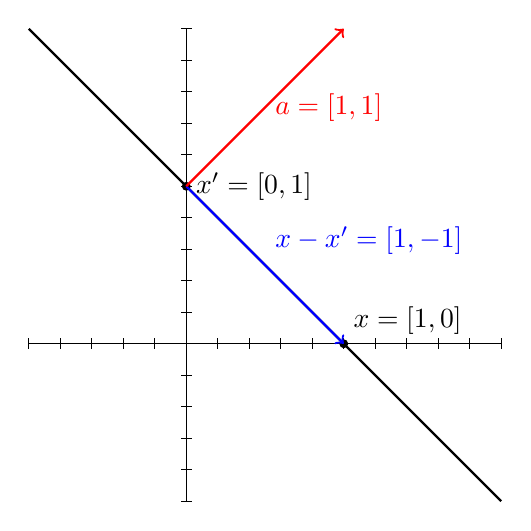
\begin{tikzpicture}[scale=2]
  %axis
  \draw (-1,0) -- coordinate (x axis mid) (2,0);
  \draw (0,-1) -- coordinate (y axis mid) (0,2);
  %ticks
  \foreach \x in {-1,-0.8,...,2}
    \draw (\x,1pt) -- (\x,-1pt);
  \foreach \y in {-1,-0.8,...,2}
  \draw (1pt,\y) -- (-1pt,\y);


  \draw[thick] (-1,2) -- (2,-1); 

  \fill (1,0) circle (.8pt) node [anchor=south west] {$x=[1,0]$};
  \fill (0,1) circle (.8pt) node [anchor=west] {$x'=[0,1]$};

  \draw[thick,->,blue] (0,1) -- node [anchor = south west] {$x-x'=[1,-1]$}  (1,0);
       
  \draw[thick,->,red] (0,1) -- node [anchor=west] {$a=[1,1]$} (1,2);

\end{tikzpicture}

\end{center}

\end{minipage}\hspace*{1cm}\begin{minipage}[t]{\textwidth-7cm}
  \vspace{0pt}
Ešte pripomeňme, že ak  sme v $m$-rozmernom priestore, nadrovina $\cal H$ je množina bodov \bm{x} spĺňajúcich
rovnosť $a_1x_1+\cdots+a_mx_m=1$ (jednotka na pravej strane je takmer všeobecná:
ľubovoľná nadrovina, ktorá neprechádza bodom $[0,\ldots,0]$ sa dá normovaním upraviť
na tento tvar). Ak označíme $\pair{\cdot}{\cdot}$ skalárny súčin, je
$\cal H$ definovaná ako $\pair{\bm{x}}{\bm{a}}=1$. 
Body, pre ktoré $\pair{\bm{x}}{\bm{a}}<1$ sú pod $\cal H$, a body
$\pair{\bm{x}}{\bm{a}}>1$ nad $\cal H$.
Vektor \bm{a} je {\em normálový vektor} $\cal H$ a pre ľubovoľné dva body \bm{x}, \bm{x'} z $\cal H$ platí,
$$\pair{\bm{x}-\bm{x'}}{\bm{a}}=\sum_{i=1}^m(x_i-x'_i)a_i=\pair{\bm{x}}{\bm{a}}-\pair{\bm{x'}}{\bm{a}}=0.$$

\noindent
V dvoch rozmeroch je nadrovinou priamka, tá na obrázku vľavo je daná rovnicou
$x_1+x_2=1$.

\end{minipage}

\noindent
Naše  úvahy o konvexných obaloch zavŕšime nasledovným pozorovaním, ktoré je
pre dva a tri rozmery úplne zjavné:

\begin{lema}
  \label{lm:KO:2}
  Majme body $\bm{x},\bm{a_1},\ldots,\bm{a_n}$ v $m$-rozmernom priestore. Nech $K$ je konvexný obal
  $\bm{a_1},\ldots,\bm{a_n}$. Potom platí:
  \begin{itemize}
    \item 
      Ak \bm{x} je vo vnútri\footnote{t.j. $K$ obsahuje \bm{x} aj nejaké jeho malé okolie} $K$,
      potom neexistuje nadrovina $\cal H$, ktorá prechádza cez \bm{x} a všetky body z $K$
      ležia na jednej strane $\cal H$.
    \item 
      Ak $\bm{x} \not\in K$,
      potom existuje nadrovina $\cal H$, ktorá prechádza cez \bm{x} a všetky body z $K$
      ležia na jednej strane $\cal H$.
  \end{itemize}
\end{lema}

\begin{dokaz}
  Prvá časť je ľahká: nech \bm{x} leží vo vnútri $K$ nech existuje taká nadrovina $\cal H$, že všetky body z $K$
  sú na jednej strane $\cal H$. Pretože $\bm{x}$ je vo vnútri $K$, existuje nejaký bod $\bm{x'}\in K$, ktorý leží
  na opačnej strane $\cal H$ ako všetky body z $K$, špeciálne ako body $\bm{a_i}$. 
  Lenže polpriestor ohraničený $\cal H$, ktorý obsahuje 
  všetky $\bm{a_i}$ je konvexné teleso, a preto z definície konvexného obalu $\bm{x'}\not\in K$.

\noindent
Ideme dokázať druhú časť.
Majme fixovaný  bod \bm{x} a pre body $\bm{y}\in K$ uvažujme euklidovskú vzdialenosť $f(\bm{y}):=||\bm{y}-\bm{x}||$. 
  Pretože $K$ je kompaktná množina a $f$ je spojitá funkcia nadobúdajúca kladné hodnoty, existuje bod
  $\bm{z}\in K$, na ktorom $f$ nadobúda minimum. Označme 
  \begin{align*}
    \bm{t}&=\bm{x}-\bm{z} & \kappa&= \pair{\bm{t}}{\bm{x}}
  \end{align*}

\begin{minipage}[t]{4.5cm}
  \vspace{0pt}
  \begin{myfig}{\textwidth}{svg/CHa}
  \end{myfig}
\end{minipage}\hspace*{1cm}\begin{minipage}[t]{\textwidth-7cm}
  \vspace{0pt}
  Nech $\cal H$ je nadrovina tvorená bodmi \bm{y}, pre ktoré $\pair{\bm{t}}{\bm{y}}=\kappa$.
  Zjavne $\bm{x}\in{\cal H}$. Platí
  $$0\le\sum_{i=1}^m(x_i-z_i)^2=%\sum_{i=1}^mx_i^2-2x_iz_i+z_i^2=
  \bpair{x}{x}-2\bpair{x}{z}-\bpair{z}{z}$$
  a preto
  \begin{align*}&\bpair{t}{z}=\pair{\bm{x}-\bm{z}}{\bm{z}}=\bpair{x}{z}-\bpair{z}{z}\le\\
                &\le\bpair{x}{x}-\bpair{x}{z}=\pair{\bm{x}-\bm{z}}{\bm{x}}=\bpair{t}{x}=\kappa
  \end{align*}
  \noindent
  Teraz stačí ukázať, že pre všetky body $\bm{y}\in K$ tiež platí $\bpair{t}{y}\le\kappa$, a teda
  ležia na rovnakej strane $\cal H$ ako \bm{z}.
\end{minipage}

\noindent
Majme teda $\bm{z}\in K$. 
Keďže \bm{z} minimalizuje vzdialenosť od \bm{x} a $K$ je konvexné teleso, pre všetky $0\le\lambda\le1$ platí
$||\bm{z}-\bm{x}||^2\le||(1-\lambda)\bm{z}+\lambda\bm{y}-\bm{x}||^2=
||(1-\lambda)(\bm{z}-\bm{x})+\lambda(\bm{y}-\bm{x})||^2$
a odtiaľ po priamočiarych úpravách
$0\le\lambda(\lambda-2)||\bm{z}-\bm{x}||^2+2\lambda(1-\lambda)\pair{\bm{z}-\bm{x}}{\bm{y}-\bm{x}}
+\lambda^2||\bm{y}-\bm{x}||^2
$.
Pretože $\lambda\ge0$, máme
$0\le(\lambda-2)||\bm{z}-\bm{x}||^2+2(1-\lambda)\pair{\bm{z}-\bm{x}}{\bm{y}-\bm{x}}
+\lambda||\bm{y}-\bm{x}||^2
$
a odtiaľ v limite pre $\lambda\mapsto0$
máme $0\le\pair{\bm{z}-\bm{x}}{\bm{y}-\bm{x}}-||\bm{z}-\bm{x}||^2
=\pair{\bm{z}-\bm{x}}{\bm{y}-\bm{x}}-\pair{\bm{z}-\bm{x}}{\bm{z}-\bm{x}}
=\pair{\bm{z}-\bm{x}}{\bm{y}}-\pair{\bm{z}-\bm{x}}{\bm{z}}=\bpair{t}{z}-\bpair{t}{y}
$.
Preto
$\bpair{t}{y}\le\bpair{t}{z}\le\kappa$, čo sme chceli dokázať.
\end{dokaz}

\end{shaded}

\noindent
Vráťme sa teraz k nášmu cieľu -- ukázať, že rovnaká hodnota
optimálneho riešenia v primárnej aj duálnej úlohe nie je náhoda. 
Pozrime sa na nasledovný príklad: Majme $m$-rozmerný priestor
$\R^m$ a v ňom $n$ bodov $\bm{a}_1,\ldots,\bm{a}_n$ (t.j. bod $\bm{a}_i$ má
súradnice $(a_{i1},a_{i2},\ldots,a_{im})$) a vektor $\bm{c}$. Cieľom je nájsť
čo najväčšie číslo $\alpha\in\R^+$ tak, že bod $\alpha\bm{c}$ leží v konvexnom
obale $K$ bodov $\bm{a}_1,\ldots,\bm{a}_n$. 

\begin{minipage}[t]{3.2cm}
  \vspace{0pt}
  \begin{myfig}{\textwidth}{svg/dualityCHa}
  \end{myfig}
\end{minipage}\hspace*{1cm}\begin{minipage}[t]{\textwidth-5cm}
  \vspace{0pt}
  \vskip 2ex
\noindent 
Predpokladajme pre jednoduchosť, že úloha má riešenie, t.j. polpriamka generovaná
vektorom \bm{c} pretína $K$. Z konvexity vyplýva, že prienik $K$ a polpriamky je úsečka.
Optimálne riešenie je preto bod $\alpha\bm{c}$, v ktorom polpriamka opúšťa $K$.
Podľa Lemy~\ref{lm:KO:1} sa 
body konvexného obalu sa dajú vyjadriť ako konvexná kombinácia bodov $\bm{a}_1,\ldots,\bm{a}_n$,
  t.j. náš hľadaný bod $\alpha\bm{c}$ sa musí dať napísať v tvare $z_1\bm{a}_1+\cdots+z_n\bm{a}_n$
  pre nejaké $z_1,\ldots,z_n\ge0$, kde $\sum_{i=1}^nz_i=1$. 
  Pre ľubovoľný prípustný bod
  $\alpha\bm{c}$ si označme  $y_j=\frac{z_j}{\alpha}$, potom
  platí 
\end{minipage}
  
  \begin{align*}
    y_j\ge&0 & \sum_{j=1}^ny_j=\frac{1}{\alpha} && \alpha\bm{c}=\alpha\sum_{j=1}^n\bm{a}_jy_j.
  \end{align*}
  Nájsť bod, pre ktorý je $\alpha$ maximálne, znamená nájsť bod, pre ktorý je $1/\alpha$ minimálne.
  Snažíme sa teda minimalizovať hodnotu $\sum_{j=1}^ny_j$ spomedzi takých $y_1,\ldots,y_n\ge 0$, 
\noindent
  pre ktoré $\sum_{j=1}^n\bm{a}_jy_j=\bm{c}$; stačí si uvedomiť, že z daných hodnôt \bm{y} vieme
  zrekonštruovať \bm{z} a $\alpha$.
Našu úlohu teda vieme zapísať ako úlohu lineárneho programovania:

\begin{equation}
  \label{eq:dualCHa}
\begin{array}{rrrrrcl}
  {\rm minimalizovať}     & y_1        & +\;y_2         & +\; \cdots  & +\;y_n   \\
  {\rm pri\ obmedzeniach} & a_{1,1}y_1 & +\;a_{2,1}y_2   & +\; \cdots  & +\;a_{n,1}y_n  & = & c_1 \\
                          & a_{1,2}y_1 & +\;a_{2,2}y_2   & +\; \cdots  & +\;a_{n,2}y_n  & = & c_2 \\
                          &   \vdots   &   \vdots       &   \ddots   &  \vdots      &  \vdots & \vdots\\ 
                          & a_{1,m}y_1 & +\; a_{2,m}y_2   & +\; \cdots  & +\;a_{n,m}y_n  & = & c_m \\
                          &\multicolumn{4}{r}{y_1,\ldots,y_n}&\ge&0
\end{array}
\end{equation}

\noindent
alebo skrátene
$$\text{(P)}\;\; \min_{\bm{y}\in\R^n}\left\{ \bm{1}\tr\bm{y} \mid A\tr\bm{y}=\bm{c},\;\bm{y}\ge\bm{0}\right\}, $$
kde $A$ je matica rozmerov $n\times m$, ktorej riadky sú tvorené súradnicami bodov $\bm{a}_1,\ldots,\bm{a}_n$.
Na program (\ref{eq:dualCHa}) použijeme náš dualizačný recept a dostaneme duálny program

\noindent
\begin{minipage}[t]{4cm}
  \vspace{0pt}
  \begin{myfig}{\textwidth}{svg/dualityCHb}
  \end{myfig}
\end{minipage}\hspace*{1cm}\begin{minipage}[t]{\textwidth-5cm}
  \vspace{0pt}

\begin{equation}
  \label{eq:dualCHb}
  \text{(D)}\;\;  \max_{\bm{x}\in\R^m}\left\{ \bm{c}\tr\bm{x} \mid A\bm{x}\le\bm{1}\right\}
\end{equation}

\noindent
Ako môžeme program (\ref{eq:dualCHb}) interpretovať? Zoberme si ľubovoľné prípustné riešenie \bm{x}. 
Nech ${\cal H}_{\bm{x}}$ je nadrovina daná bodmi \bm{y}, pre ktoré $\bpair{y}{x}=1$.
Obmedzenia programu (\ref{eq:dualCHb}) hovoria, že pre každý bod $\bm{a_i}$ je 
$\bpair{a_i}{x}\le1$, a z konvexity je preto celý konvexný obal $K$ pod ${\cal H}_{\bm{x}}$.
Ďalej ak označíme $\alpha=\frac{1}{\bm{c}\tr\bm{x}}$, tak  bod $\alpha\bm{c}$ leží v nadrovine 
${\cal H}_{\bm{x}}$, lebo $\pair{\alpha\bm{c}}{\bm{x}}=1$. Každému prípustnému riešeniu (\ref{eq:dualCHb})
teda zodpovedá bod $\alpha\bm{c}$ na polpriamke generovanej vektorom \bm{c}, ktorý (podľa Lemy~\ref{lm:KO:2})
neleží vo vnútri $K$.
Naviac je zrejmé, že optimálne riešenie je nezáporné, a preto môžme bez ujmy na všeobecnosti predpokladať,
že $\bpair{x}{c}=||\bm{x}||\cdot||\bm{c}||\cos\varphi\ge0$, kde $\varphi$ je uhol, ktorý zvierajú
vektory \bm{x} a \bm{c}. Preto nás zaujímajú iba tie prípustné riešenia, ktorým zodpovedajú
body $\alpha\bm{c}$ ležiace na polpriamke generovanej \bm{c} za $K$.
\end{minipage}

\vspace*{-4ex}
\noindent
Platí to aj naopak. Zoberme si hocijaký bod $\alpha\bm{c}$ ležiaci za $K$. Podľa Lemy~\ref{lm:KO:2}
existuje nadrovina $\cal H$ taká, že všetky body z $K$ ležia pod ňou. Nech $\cal H$ je tvorená
bodmi \bm{y} spĺňajúcimi $\bpair{x}{y}=1$ pre nejaký vektor \bm{x}, potom platí $A\bm{x}\le1$.
Zároveň, pretože $\cal H$ prechádza cez $\alpha\bm{c}$, platí 
$\pair{\bm{x}}{\alpha\bm{c}}=1=\alpha\bpair{x}{c}$, a teda $\alpha=\frac{1}{\bm{c}\tr\bm{x}}$.
Pre maximálnu hodnotu $\bm{c}\tr\bm{x}$ je príslušná $\alpha$ minimálna, a preto program (\ref{eq:dualCHb})
vyžaduje nájsť minimálne $\alpha$ tak, aby bol $\alpha\bm{c}$ ležal za $K$ na polpriamke generovanej 
vektorom \bm{c}. To je ale zjavne bod, v ktorom polpriamka opúšťa $K$, a teda programy
(\ref{eq:dualCHa}) a (\ref{eq:dualCHb}) majú rovnaké optimálne riešenie.
Dokázali sme teda tvrdenie

\begin{lema}
  \label{lm:strongdualityprep}
  Ak primárny program $\min_{\bm{y}\in\R^n}\left\{ \bm{1}\tr\bm{y} \mid A\tr\bm{y}=\bm{c},\;\bm{y}\ge\bm{0}\right\}$
má prípustné riešenie, potom aj duálny program 
$\max_{\bm{x}\in\R^m}\left\{ \bm{c}\tr\bm{x} \mid A\bm{x}\le\bm{1}\right\}$
má prípustné riešenie a optimálne hodnoty oboch programov sa rovnajú.
\end{lema}

\noindent
Keby sa nám podarilo Lemu~\ref{lm:strongdualityprep}
zovšeobecniť na programy tvaru  
$\min_{\bm{y}\in\R^n}\left\{ \bm{b}\tr\bm{y} \mid A\tr\bm{y}=\bm{c},\;\bm{y}\ge\bm{0}\right\}$
pre ľubovoľný vektor \bm{b},
boli by sme spokojní, lebo každý lineárny program sa dá napísať v takomto tvare. 
Majme teda primárny program
\begin{equation}
  \label{eq:dualgenP}
  \text{(P)}\;\; \min_{\bm{y}\in\R^n}\left\{ \bm{b}\tr\bm{y} \mid A\tr\bm{y}=\bm{c},\;\bm{y}\ge\bm{0}\right\}
\end{equation}
a k nemu duálny program
\begin{equation}
  \label{eq:dualgenD}
  \text{(D)}\;\;\max_{\bm{x}\in\R^m}\left\{ \bm{c}\tr\bm{x} \mid A\bm{x}\le\bm{b}\right\}\hspace*{10ex}
\end{equation}
\noindent
Uvažujme najprv vektory \bm{b} také, že všetky zložky $b_i>0$.
Označme 
\begin{align}
  \label{eq:dualgenNote1}
  \bm{a}_i'=&\frac{1}{b_i}\bm{a}_i & y_j'=&b_jy_j 
\end{align}

\noindent
Platí $\bm{b}\tr\bm{y}=\sum_{j=1}^nb_jy_j=\bm{1}\tr\bm{y}'$ a pre každé $i\in\{1,\ldots,m\}$
$\sum_{j=1}^ma_{ji}y_j=\sum_{j=1}^ma'_{ji}b_i\frac{y_j'}{b_j}$. Pretože $b_j>0$,  program (\ref{eq:dualgenP})
je ekvivalentný\footnote{v tom zmysle, že každému riešeniu programu (\ref{eq:dualgenP}) prislúcha nejaké riešenie 
programu (\ref{eq:dualgen3}) s rovnakou hodnotou a naopak}s programom
\begin{equation}
  \label{eq:dualgen3}
  \min_{\bm{y'}\in\R^n}\left\{ \bm{1}\tr\bm{y'} \mid A'\bm{y'}=\bm{c},\;\bm{y'}\ge\bm{0}\right\} 
\end{equation}
kde stĺpce matice  $A'$ sú vektory $\bm{a}_i'$.
Podľa Lemy~\ref{lm:strongdualityprep}, ak má program (\ref{eq:dualgen3}) prípustné riešenie, tak jeho optimum
je rovnaké ako optimum programu
\begin{equation}
  \label{eq:dualgen4}
  \max_{\bm{x'}\in\R^m}\left\{ \bm{c}\tr\bm{x'}\mid {A'}\tr\bm{x'}\le\bm{1}\right\}
 \end{equation}
 Obmedzenia programu (\ref{eq:dualgen4}) sú v tvare $\sum_{j=1}^ma_{ji}'x'_j\le1$ a tak s použitím
 označenia (\ref{eq:dualgenNote1}) dostávame, že programy (\ref{eq:dualgen4}) a (\ref{eq:dualgenD}) sú ekvivalentné,
 preto ak (\ref{eq:dualgenP}) má prípustné riešenie, má ho aj (\ref{eq:dualgenD}) a hodnoty optima sú rovnaké.

\begin{prob}
  Upravte predchádzajúci postup tak, aby platil pre $b_i\ge0$.
\end{prob}

\noindent
Nech teraz \bm{b} nadobúda ľubovoľné hodnoty a nech $\bm{\tilde{x}}$ je prípustné riešenie (\ref{eq:dualgenD}).
Označme 
\begin{align}
  \label{eq:dualgen5}
  \bm{x'}&=\bm{x}-\bm{\tilde{x}} & b_i'&=b_i-\bm{a}_i\tr\bm{\tilde{x}}
\end{align}

\noindent
Ako sa v tomto označení zmenia programy (\ref{eq:dualgenP}) a (\ref{eq:dualgenD})?
Pre prípustné riešenia \bm{x}, \bm{y} platí
$$
\begin{array}{ll}
  \bm{c}\tr\bm{x} &= \bm{c}\tr\bm{x'} + \bm{c}\tr\bm{\tilde{x}}\\
  \bm{b}\tr\bm{y} &= \sum_{i=1}^nb_iy_i = \sum_{i=1}^nb'_iy_i+\sum_{i=1}^ny_i(\bm{a}_i\tr\bm{\tilde{x}})=
  \bm{b'}\tr\bm{y}+\sum_{i=1}^ny_i\sum_{j=1}^ma_{i,j}\tilde{x}_j =\\
  &= \bm{b'}\tr\bm{y}+ \sum_{j=1}^m\tilde{x}_j(\sum_{i=1}^ny_ia_{i,j}) =
  \bm{b'}\tr\bm{y}+\bm{c}\tr\bm{\tilde{x}}
\end{array}
$$
kde posledná rovnosť vyplýva z toho, že $A\tr\bm{y}=\bm{c}$. 
Pretože $\bm{c}\tr\bm{\tilde{x}}$ je konštanta, programy  (\ref{eq:dualgenP}) a (\ref{eq:dualgenD}) vieme 
ekvivalentne zapísať ako
\begin{align*}
  (\text{P}')\;\; \min_{\bm{y}\in\R^n}\left\{ \bm{b'}\tr\bm{y} \mid A\tr\bm{y}=\bm{c},\;\bm{y}\ge\bm{0}\right\}
  &&
 (\text{D}')\;\; \max_{\bm{x'}\in\R^m}\left\{ \bm{c}\tr\bm{x'} \mid A\bm{x'}\le\bm{b'}\right\}
\end{align*}

\noindent
Navyše z prípustnosti $\bm{\tilde{x}}$ pre (\ref{eq:dualgenD}) vyplýva, že $\bm{b'}\ge\bm{0}$ a preto
môžeme aplikovať predchádzajúci prípad.

\noindent
Načrtli sme\footnote{pre kompletný dôkaz treba ošetriť ešte niekoľko 
špeciálnych prípadov, ktoré prenechávame na čitateľa} dôkaz fundamentálnej vety v teórii lineárneho programovania:

\begin{framed}
  \begin{veta}[Silná veta o dualite]
    \label{thm:strongduality}
    Pre dvojicu duálnych lineárnych programov
    \begin{align*}
      \text{(P)}\;\; \min_{\bm{y}\in\R^n}\left\{ \bm{b}\tr\bm{y} \mid A\tr\bm{y}=\bm{c},\;\bm{y}\ge\bm{0}\right\}
      &&
      \text{(D)}\;\;\max_{\bm{x}\in\R^m}\left\{ \bm{c}\tr\bm{x} \mid A\bm{x}\le\bm{b}\right\}\hspace*{10ex}
    \end{align*}
    Platí práve jedna zo štyroch možností:
    \begin{enumerate}
      \item (P) ani (D) nemajú žiadne prípustné riešenie
      \item (P) je neohraničený a (D) nemá prípustné riešenie
      \item (D) je neohraničený a (P) nemá prípustné riešenie
      \item (P) aj (D) majú prípustné riešenie. V tom prípade sa optimálne hodnoty (P) a (D) rovnajú.
    \end{enumerate}
  \end{veta}
\end{framed}

 
\section{\maxflow--\mincut očami duality}

\noindent Dualita lineárneho programovania, ktorú sme predstavili v
predchádzajúcej časti, často pomáha lepšie pochopiť min--max charakterizácie
výpočtových problémov.  V tejto časti si z pohľadu duality priblížime známe
tvrdenie, že veľkosť maximálneho toku sa rovná kapacite minimálneho rezu.


\noindent
Začneme tým, že predstavíme problém maximálneho toku. Keďže predpokladáme, že čitateľ
sa s ním už stretol, odpustíme si tentokrát motivačné rozprávky a zopakujeme len definíciu. 
Majme daný (neorientovaný) graf $G=(V,E)$ s nezápornými váhami hrán, t.j. 
funkciou $c:E\mapsto\R^+$; namiesto $c(\{u,v\})$ budeme skrátene písať $c_{uv}=c_{vu}$.
V grafe sú dva význačné vrcholy $s$ a $t$.
V probléme \maxflow je cieľom nájsť čo najväčší tok z $s$ do $t$. Tok je funkcia 
$f:V^2\mapsto\R^+$, ktorej interpretácia je taká, že $f(u,v)$ je množstvo kvapaliny, ktorá tečie
z $u$ do $v$. Funkcia $f$ musí spĺňať tieto vlastnosti:
\begin{enumerate}
  \item ak $f(u,v)\not=0$, potom $(u,v)\in E$, t.j. tiecť musí po hranách grafu
  \item $f(u,v)=-f(v,u)$, t.j. znamienko udáva, ktorým smerom tok ide
  \item pre každé $v\not\in\{s,t\}$ platí $\sum\limits_{u\in V}f(u,v)=0$, t.j. čo do vrchola vteká, to z neho aj vytečie
\end{enumerate}
\noindent
Veľkosť toku je $\sum_{v\in V}f(s,v)$. Rez v grafe $G$ je množina hrán, ktorej odobratie oddelí vrcholy $s$ a $t$.
Cena rezu je súčet váh prerezaných hrán. Problém \mincut je nájsť rez minimálnej ceny. 
Na nasledovnom obrázku je graf s kapacitami hrán a minimálnym rezom (vľavo) a maximálnym tokom 
(vpravo; tmavo sú označené hrany, ktorých kapacita je naplnená tokom) s hodnotou 24.


\begin{myfig}{\textwidth}{svg/flowcutNew}
\end{myfig}


\noindent
Problém \maxflow sa dá prirodzene formulovať ako úloha lineárneho programovania, a to hneď niekoľkými
spôsobmi. Z dôvodov, ktoré, ako dúfame, budú jasné na konci tejto časti, si zvolíme takúto 
formuláciu: pre každú hranu $(u,v)\in E$ budeme mať dve nezáporné premenné $x_{uv}$ a $x_{vu}$, 
ktoré budú udávať množstvo toku z $u$ do $v$ (všimnite si, že sme tým povolili situáciu, 
že po tej istej hrane tečie tok oboma smermi: $x_{uv}$ v smere z $u$ do $v$ a $x_{vu}$ v
smere z $v$ do $u$; ničmenej, tieto dve hodnoty stačí odčítať a dostaneme riešenie
v zmysle našej definície). Ďalej budeme mať jednu premennú $f$, ktorá bude udávať veľkosť
toku (a tú sa budeme snažiť maximalizovať): $f=\sum\limits_{u:(s,u)\in E}x_{su}-\sum\limits_{u:(s,u)\in E}x_{us}$. 
Zákony zachovania toku aj obmedzenia kapacít  
ľahko zapíšeme pomocou lineárnych nerovností a dostaneme program

\begin{equation}
  \label{eq:flow:1}
  \begin{array}{rrcll}
      {\rm maximalizovať}     & \multicolumn{1}{r}{f}\\[8mm]
    {\rm pri\ obmedzeniach} & \sum\limits_{u:(s,u)\in E} x_{su} - \sum\limits_{u:(s,u)\in E} x_{us} - f  &=&0&  \\[6mm]
                            & \sum\limits_{u:(t,u)\in E} x_{ut} - \sum\limits_{u:(s,u)\in E} x_{tu} + f  &=&0&  \\[6mm]
                            & \sum\limits_{u:(u,v)\in E} x_{vu} - \sum\limits_{u:(u,v)\in E} x_{uv} &=&0&\;\;\;
    \forall v\in V - \{s,t\}\\[6mm]
    & x_{uv}&\le& c_{uv}&  \;\;\;\forall (u,v)\in E\\[1mm]
    & x_{vu}&\le& c_{uv}&  \;\;\;\forall (u,v)\in E\\[1mm]
                            & x_{uv}&\ge& 0 &  \;\;\;\forall (u,v)\in E\\
  \end{array}
\end{equation}  

\noindent
Prvé a druhé obmedzenie definujú veľkosť toku $f$ ako to, čo vyteká z $s$, resp. čo vteká do $t$. Vo všetkých
ostatných vrcholoch platí zákon zachovania toku. 

\noindent
Použime teraz náš dualizačný recept a zostrojme k programu (\ref{eq:flow:1}) duálny minimalizačný program. 
Každému obmedzeniu v primárnom programe zodpovedá premenná v duálnom programe.
V programe (\ref{eq:flow:1}) máme dva druhy obmedzení: obmedzenia v tvare $\cdots = 0$ pre každý vrchol
a obmedzenia $x_{uv}\le c_{uv}$. Zavedieme si preto duálne premenné $y_v\in\R$ pre každý vrchol $v\in V$
($y_s$ zodpovedá prvému obmedzeniu, $y_t$ druhému a ostatné $y_v$ v poradí ďalším)
a premenné $z_{uv}$ a $z_{vu}$ pre každú hranu $(u,v)\in E$, pričom $z_{uv},z_{vu}\ge0$.
Duálny program sa vyrába tak, že $i$-ta duálna premenná je  multiplikátor, ktorým prenásobíme
$i$-te obmedzenie a výsledky sčítame; súčet pravých strán je príslušný odhad a vyžadujeme, aby
súčet ľavých strán bol v každej zložke väčší ako maximalizovaná funkcia.
Súčet pravých strán je v našom prípade $\sum\limits_{(u,v)\in E}(z_{uv}+z_{vu})c_{uv}$.
Maximalizovaná funkcia má pri všetkých premenných okrem $f$ hodnotu 0. 
Premenná $f$ vystupuje iba v prvom a druhom obmedzení (\ref{eq:flow:1}), preto dostávame
v duálnom programe obmedzenie $y_t-y_s=1$ (je jasné, že tok je nezáporný, ale formálne sme 
v (\ref{eq:flow:1}) nevyžadovali, aby $f\ge0$). Každá premenná $x_{uv}$ sa vyskytuje v 
dtroch obmedzeniach: v obmedzení zodpovedajúcom vrcholu $u$ s kladným znamienkom,  v obmedzení
zodpovedajúcom vrcholu $v$ so záporným znamienkom a v obmedzení $x_{uv}\le c_{uv}$. Dostávame
tak duálny program


\begin{equation}
  \label{eq:flow:2}
  \begin{array}{rrcll}
    {\rm minimalizovať}     & \multicolumn{1}{r}{\sum\limits_{(u,v)\in E}(z_{uv}+z_{vu})\,c_{uv}}\\[8mm]
    {\rm pri\ obmedzeniach} & y_t - y_s  &=&1&  \\[3mm]
                            & y_v - y_u + z_{uv} &\ge&0&\;\;\;    \forall (u,v)\in E \\[3mm]
                            & y_u - y_v + z_{vu} &\ge&0&\;\;\;    \forall (u,v)\in E \\[3mm]
                            & z_{uv},z_{vu}&\ge& 0 &  \;\;\;\forall (u,v)\in E\\
  \end{array}
\end{equation}  

\noindent
Z vety o dualite vieme, že programy (\ref{eq:flow:1}) a (\ref{eq:flow:2}) majú rovnakú hodnotu optima. 
Ako môžme program (\ref{eq:flow:2}) interpretovať? 
Bez ujmy na všeobecnosti môžme predpokladať, že aspoň jedna z dvojice premenných $z_{uv},z_{vu}$
je nulová: jediné obmedzenia na $z_{uv}$ a $z_{vu}$
sú $z_{uv}\ge y_u-y_v$ a $z_{vu}\ge y_v-y_u$. Zjavne aspoň jedna z hodnôt $y_u-y_v$ a $y_v-y_u$
nie je kladná, a teda ak máme ľubovoľné prípustné riešenie, tak aspoň jednu z premenných 
$z_{uv},z_{vu}$ môžme nastaviť na 0 a nezväčšíme hodnotu minimalizovanej funkcie. 
Môžme si preto označiť $\bar{z}_{uv}=\max\{z_{uv},z_{vu}\}$; obmedzenia potom hovoria, že
$\bar{z}_{uv}\ge|y_u-y_v|$ a z rovnakých dôvodov ako pred chvíľou môžeme bez ujmy na všeobecnosti
predpokladať, že $\bar{z}_{uv}=|y_u-y_v|$. Môžme si predstaviť, že vrcholy grafu ukladáme 
na priamku: vrchol $v$ je uložený v bode $y_v$, pričom, opäť bez ujmy na všeobecnosti, je $s$ uložený
v bode 0 a $t$ v bode 1. $\bar{z}_{uv}$ je dĺžka hrany $(u,v)$ v našom uložení.
Keď to zhrnieme, optimálne riešenie programu (\ref{eq:flow:2}) nám dá také uloženie vrcholov grafu na 
úsečku dĺžky 1, že $s$ a $t$
sú na krajoch a minimalizuje sa váhovaná dĺžka hrán.

\begin{myfig}{0.9\textwidth}{svg/relaxcut}
  Graf s váhami hrán a jedno z možných optimálnych riešení programu (\ref{eq:flow:2}):
  $\bar{z}_{su}=\bar{z}_{vw}=\frac{1}{6}$, $\bar{z}_{sv}=\bar{z}_{uw}=\frac{1}{3}$,
  $\bar{z}_{sw}=\bar{z}_{wt}=\frac{1}{2}$. Výsledná hodnota je
  $$\sum_{(u,v)\in E}c_{uv}\bar{z}_{uv}=\frac{1}{6}+\frac{1}{3}+2\frac{1}{2}+\frac{1}{3}+\frac{1}{6}+4\frac{1}{2}=4.$$
\end{myfig}

\noindent
Poďme teraz prepísať program (\ref{eq:flow:2}) do normálneho tvaru 
$\max\{-\bm{c}\tr\bm{\beta}\mid A\bm{\beta}=0,\;\bm{\beta}\ge0\}$.
Ku každej premennej $z_{uv}$ zavedieme premennú $\hat{z}_{uv}\ge 0$, aby sme získali
obmedzenia tvaru \hbox{$y_v-y_u+z_{uv}-\hat{z}_{uv}=0$}.
Ak vektor  $\bm{\beta}$  pozostáva zaradom z hodnôt 
$y_s,y_t,y_{v_1},\ldots,z_{uv},z_{vu},\ldots,\hat{z}_{uv}.\hat{z}_{vu},\ldots$, 
matica $A$ má takúto štruktúru:

\begin{myfig}{0.8\textwidth}{svg/cutlp}
\end{myfig}

\noindent
Nasledujúcu priamočiaru povinnú jazdu prenecháme na čitateľa:

\begin{prob}
  S pomocou viet \ref{thm:idTum} a \ref{thm:unimod} ukážte, že matica $A$ je TUM.
\end{prob}


\noindent
Z Vety~\ref{thm:tumInteger} vyplýva, že existuje celočíselné optimálne riešenie programu (\ref{eq:flow:2}).
To znamená, že všetky vrcholy majú $y_v\in\{0,1\}$ (t.j. sú uložené na niektorom konci úsečky)
a každá hrana má dĺžku 0 alebo 1. Preto každá cesta z $s$ do $t$ musí obsahovať aspoň jednu hranu s dĺžkou $1$,
a teda ak hrany dĺžky 1 z grafu odstránime, dostaneme rez, ktorý oddeľuje $s$ od $t$. Môžme teda povedať

\begin{veta}[\maxflow-\mincut veta]
  Veľkosť maximálneho toku sa rovná kapacite minimálneho rezu.
\end{veta}
\begin{dokaz}
  Veľkosť maximálneho toku je optimum programu (\ref{eq:flow:1}), ktoré je rovnaké, ako optimum
  programu (\ref{eq:flow:2}). Existuje celočíselné optimum programu (\ref{eq:flow:2}), a zároveň
  je bijekcia medzi $s-t$ rezmi a celočíselnými riešeniami  (\ref{eq:flow:2}): celočíselnému riešeniu
  (\ref{eq:flow:2}) prislúcha rez a každému rezu vieme prirodzeným spôsobom priradiť riešenie  (\ref{eq:flow:2}).
\end{dokaz}

\noindent
Je dosť možné, že čitateľ možno pozná oveľa jednoduchší dôkaz tohto tvrdenia. Dôvod, prečo uvádzame tento dôkaz je
(okrem toho, že chceme ilustrovať dualitu lineárnych programov) ten, že ukazuje dvojicu 
\maxflow-\mincut ako špeciálny prípad všeobecnejších problémov; zároveň dáva nový pohľad na otázku, prečo
rovnaký výsledok neplatí pre iné podobné problémy (ak napríklad máme viacero zdrojov a ústí a cieľom je
maximalizovať tok rôznych komodít v spoločných potrubiach, máme duálany problém k problému
\minmulticut z Definície~\ref{dfn:multicut}, avšak analogický výsledok neplatí) cez unimodularitu príslušných matíc.

 
\section{Primárno-duálna metóda}

\noindent
Dúfame, že sme čitateľa presvedčili o tom, že dualita je zaujímavá vlastnosť lineárnych
programov. Teraz je načase ukázať, ako sa dá využiť pri návrhu algoritmov. Pozrime sa na dvojicu
duálnych programov
\begin{eqnarray*}
  (P):&\min\limits_{\bm{x}\in\R^n}\{\bm{c}\tr\bm{x}\mid A\bm{x}\ge\bm{b}, \bm{x}\ge 0\}\\
  (D):&\max\limits_{\bm{y}\in\R^m}\{\bm{b}\tr\bm{y}\mid A\tr\bm{y}\le\bm{c}, \bm{y}\ge 0\}
\end{eqnarray*}

\noindent
Z vety o dualite vieme, že majú rovnakú hodnotu optima, t.j. že existujú vektory $\bm{x^\star}\ge0$
a $\bm{y^\star}\ge0$, že 
$A\bm{x^\star}\ge\bm{b}$, $A\tr\bm{y^\star}\le\bm{c}$
a
$\bm{c}\tr\bm{x^\star}=\bm{b}\tr\bm{y^\star}$.
Pripomeňme si nerovnosti z dôkazu Vety~\ref{thm:weakduality}, ktoré platia pre všetky dvojice prípustných
riešení primárnej a duálnej úlohy, a teda aj pre $\bm{x^\star}$, $\bm{y^\star}$:

\begin{equation}
  \label{eq:proofSlack}
  \bm{c}\tr\bm{x^\star}\stackrel{(\clubsuit)}{\ge}\left(A\tr\bm{y^\star}\right)\tr\bm{x^\star}
=\bm{y^\star}\tr A\bm{x^\star}\stackrel{(\diamondsuit)}{\ge}\bm{y^\star}\tr\bm{b}
\end{equation}

\noindent
Keďže $\bm{c}\tr\bm{x^\star}=\bm{b}\tr\bm{y^\star}$, $(\clubsuit)$ aj $(\diamondsuit)$ musia
byť rovnosti. Pozrime sa na $(\clubsuit)$ a rozpíšme vektorový zápis pomocou sumy:

\begin{equation}
  \label{eq:kompl:1}
  \sum_{j=1}^n c_jx^\star_j=\sum_{j=1}^n\left[A\tr\bm{y^\star}\right]_jx^\star_j,
\end{equation}

\noindent
kde symbol $[\cdot]_j$ označuje $j$-ty prvok vektora. Z prípustnosti duálneho riešenia vieme, že
$\bm{c}\ge A\tr\bm{y^\star}$; nerovnosť vektorov platí v každej zložke, takže pre každé $j$ je
$c_j\ge\left[A\tr\bm{y^\star}\right]_j$.
Pre každé $j$ je  $x^\star_j\ge0$, a teda aj $c_jx^\star_j\ge\left[A\tr\bm{y^\star}\right]_jx^\star_j$.
Z toho vidieť, že ak má platiť rovnosť (\ref{eq:kompl:1}), musí platiť rovnosť v každej zložke.

\noindent
Rovnaké úvahy sa dajú urobiť pre nerovnosť $(\diamondsuit)$ a dostaneme tak nasledovnú charakterizáciu
optimálneho riešenia:

\begin{framed}
\begin{veta}[podmienky komplementarity]
  \label{thm:slackness}
Nech \bm{x}, \bm{y} sú prípustné riešenia primárnej a duálnej úlohy. 
Potom \bm{x}, \bm{y} sú obidve optimálne {\bf vtedy a len vtedy}, ak
sú splnené obe nasledujúce podmienky:

\begin{itemize}
\item primárna podmienka komplementarity:
$$\forall\;1\le j\le n:\;{\rm\ buď\ }\; x_j=0\; {\rm\ alebo\ }\sum_{i=1}^ma_{ij}y_i=c_j$$
\item duálna podmienka komplementarity:
$$\forall\;1\le i\le m:\;{\rm\ buď\ }\; y_i=0\; {\rm\ alebo\ }\sum_{j=1}^na_{ij}x_j=b_i$$
\end{itemize}
\end{veta}
\end{framed}

\subsection*{Edmondsov algoritmus pre \minfactor}

\noindent
Podmienky komplementarity sú užitočný nástroj pri analýze algoritmov, lebo poskytujú jednoduchý invariant,
ktorý charakterizuje optimum. Pripomeňme si definíciu problému\\ \maxWBmatching z časti o ILP:

{
  \renewcommand{\thedummy}{\ref{dfn:maxWBmatching}}
  \begin{dfn}
    Majme daný bipartitný graf s hranami ohodnotenými nezápornými reálnymi
    číslami. Cieľom problému \maxWBmatching je nájsť množinu hrán s najväčším
    súčtom váh tak, aby žiadne dve vybraté hrany nezdieľali vrchol.
  \end{dfn}
}

\noindent
Problém sme vtedy formulovali ako celočíselný program

\begin{equation*}
\begin{array}{rrcll}
  {\rm maximalizovať}     & \multicolumn{1}{l}{\sum\limits_{e\in E}\omega_ex_e}\\[3ex]
  {\rm pri\ obmedzeniach} & \sum\limits_{e\in E\atop e=(v,w)}x_e&\le&1& \;\;\;\forall v\in V\\
                          & x_e&\ge&0& \;\;\;\forall e\in E\\
                          & x_e&\in&\Z
\end{array}
\end{equation*}

\noindent
kde $\bm{\omega}\in\R^n$ je vektor váh hrán. Ukázali sme, že matica obmedzení je TUM, a preto stačí vyriešiť 
relaxovaný program a podmienky celočíselnosti máme zadarmo. Celkom prirodzene sa natíska otázka: 
''{\em A čo keby ten graf nebol bipartitný?}'' Formulácia ILP bude stále v poriadku, ale už nebude platiť, že
musí existovať optimálne celočíselné riešenie.


\begin{myfig}{0.8\textwidth}{svg/matchingLP}
  Vľavo je graf s váhami hrán. Maximálne párovanie má hodnotu $21$: hrany váhy $10$ sú iba medzi vrcholmi 
  $\{p,q,r,s,t\}$, t.j. môžu byť v riešení najviac dve. Zo zvyšných hrán môže byť najviac 1.
  Vpravo riešenie relaxovaného programu s hodnotou $25$.
\end{myfig}

\noindent
Prv, než budeme pokračovať, upravíme trocha formuláciu nášho problému. Párovaniu, ktoré pokrýva všetky hrany,
t.j. takej množine hrán $E'\subseteq E$, že každý vrchol susedí s práve jednou hranou z $E'$, 
budeme hovoriť {\em perfektné párovanie}, respektíve {\em 1-faktor} (pochopiteľne, aby graf mal 1-faktor,
musí mať párny počet vrcholov). Namiesto hľadania najťažšieho párovania
nám stačí vedieť hľadať najťažší 1-faktor: z grafu $G$ vyrobíme $G'$ tak, že ak má  $G$ nepárny počet 
vrcholov, pridáme k nemu jeden izolovaný vrchol a potom všetky vrcholy, ktoré nie sú spojené hranou spojíme
hranou váhy 0. Čitateľ sa ľahko presvedčí, že párovania v $G$ zodpovedajú 1-faktorom v $G'$.

\noindent
Ďalej nech $\omega_{\max}$ je maximálna váha hrany v $G'$. Ak vyrobíme $G''$ tak, že
nastavíme nové váhy $\omega''_e=\omega_{\max}-\omega_e$, tak vidno, že najľahší 1-faktor v $G''$ je 
najťažší 1-faktor v $G''$. Dostali sme sa tak k nasledovnej definícii:

\begin{framed}
  \begin{dfn}
    \label{dfn:minFactor}
    Majme daný úplný ohodnotený graf $G=(V,E)$ na $n=2k$ vrcholoch, pričom hrana
    $e=(u,v)\in E$ má váhu $\omega_e\in\R^+$.  Problém \minfactor je 
    nájsť 1-faktor v $G$, pre ktorý je súčet váh hrán
    minimálny, t.j.
    $\min_{E'}\sum_{e\in E'}\omega_e,$
    kde minimum je brané cez všetky 1-faktory $E'$.\end{dfn}\end{framed}


\noindent
Čitateľ, ktorý s nami vydržal až potiaľto, určite nebude mať ťažkosti zapísať \minfactor ako celočíselný
lineárny program:
pre každú hranu $e\in E$ zavedieme premennú $x_e\in\{0,1\}$, ktorá
vyjadruje, či je hrana $e$ vybratá do párovania alebo nie.
Vybratá množina hrán je 1-faktor práve vtedy, ak s každým vrcholom susedí práve jedna vybratá
hrana, čo priamočiaro zapíšeme

\begin{equation}
  \label{eq:1f:ILP}
\begin{array}{rrcll}
  {\rm minimalizovať}     & \multicolumn{1}{l}{\sum\limits_{e\in E}\omega_ex_e}\\[3ex]
  {\rm pri\ obmedzeniach} &  \sum\limits_{e\in E\atop e=(u,v)} x_e &=&1& \;\;\;\forall v\in V\\
                          & x_e&\in&\{0,1\}& \;\;\;\forall e\in E\\
\end{array}
\end{equation}

\noindent
Ak tento program relaxujeme a namiesto $x_e\in\{0,1\}$ budeme požadovať iba $x_e\ge0$ 
(čitateľ si všimne, že $x_e\le1$ vyplýva z minimality), optimum už nemusí byť celočíselné. 
V nasledujúcich odstavcoch predstavíme primárno-duálny prístup podľa Edmondsa \cite{Edmonds65} \FIXME{citat neexistuje}.
Najprv ale ešte jedno označenie, ktoré nám zjednoduší zápis:

\begin{dfn}[hranová hranica množiny]
  \label{dfn:edgeboundary}
Majme graf $G=(V,E)$ a množinu vrcholov $S\subseteq V$. Hranová hranica množiny S, označovaná $\delta(S)$, je množina hrán 
s jedným koncom v $S$ a druhým mimo $S$, t.j.:
$$\delta(S):=\{e\in E\mid e=(u,v),\;u\in S,\;v\in V\setminus S\}$$
\end{dfn}

\noindent
Ako sa vysporiadať s tým, že relaxácia programu (\ref{eq:1f:ILP}) nemá celočíselné riešenie? Trik je v tom,
že pridáme (veľa) dodatočných obmedzení, ktoré zabezpečia celočíselnosť optima. Nech \S
sú všetky aspoň trojprvkové 
množiny s nepárnym počtom vrcholov, t.j.

$$\S:=\left\{ S\subseteq V\mid\; |S|>1,\;|S|\;\text{\ nepárne\ }\right\}$$

\noindent
Každá hrana má dva konce, a preto vrcholy z $S\in\S$ nemôžu byť popárované medzi sebou, takže
v každom 1-faktore musí aspoň 1 hrana odchádzať z $S$. Pridáme tieto obmedzenia k relaxovanému programu
(\ref{eq:1f:ILP}),
čím dostaneme

\begin{equation}
  \label{eq:1f:P}
\begin{array}{rrcll}
  {\rm minimalizovať}     & \multicolumn{1}{l}{\sum\limits_{e\in E}\omega_ex_e}\\[4ex]
  {\rm pri\ obmedzeniach} &  \sum\limits_{e\in\delta(\{v\})} x_e &=&1& \;\;\;\forall v\in V\\[4ex]
                          & \sum\limits_{e\in\delta(S)}x_e&\ge&1&\;\;\;\forall S\in\S\\[4ex]
                          & x_e&\ge&0& \;\;\;\forall e\in E\\
\end{array}
\end{equation}

\noindent
\ldots a {\em voilà!} Máme lineárny program, ktorý má celočíselné optimálne riešenie.
Dostali sme sa však z dažďa pod odkvap: po prvé potrebujeme dokázať, že naozaj existuje
celočíselné optimum programu (\ref{eq:1f:P}) a podruhé potrebujeme riešiť program, ktorý má 
exponenciálne veľa obmedzení. Ani jeden z týchto problémov nie je neprekonateľný, ale my
to spravíme elegantne: využijeme dualitu a vyhneme sa riešeniu (\ref{eq:1f:P}); a navyše 
dôkaz celočíselnosti vypadne zadarmo.
Spôsob návrhu algoritmov, ktorý tu ukážeme, sa zvykne nazývať {\em primárno-duálna metóda}.

\noindent
Použime náš dualizačný recept a zostrojme duálny program k (\ref{eq:1f:P}).
Duálny program bude maximalizačný a bude mať premennú pre každé obmedzenie. Máme dva typy
obmedzení: pre vrcholy a pre množiny, takže si zavedieme duálne premenné $r_v\in\R$ pre $v\in V$
a premenné $w_S\in\R^+$ pre $S\in\S$.
Každá primárna premenná  $x_e$ má vklad $x_e\omega_e$ do minimalizačnej funkcie a vyskytuje
sa v dvoch obmedzeniach pre vrcholy (konkrétne pre dva koncové vrcholy $e$) a v obmedzeniach
pre tie množiny $S\in\S$, kde $e\in\delta(S)$.
Dostali sme duálny program (všimnite si, že $r_v$ môže byť aj záporné):

\begin{equation}
  \label{eq:1f:D}
\begin{array}{rrcll}
  {\rm maximalizovať}     & \multicolumn{1}{l}{\sum\limits_{v\in V}r_v + \sum\limits_{S\in\S}w_S}\\[4ex]
  {\rm pri\ obmedzeniach} & 
        r_u + r_v + \sum\limits_{S\in\S\atop e\in\delta(S)} w_S &\le&\omega_e& \;\;\;\forall e=(u,v)\in E\\[4ex]
                          & w_S&\ge&0& \;\;\;\forall S\in\S\\
\end{array}
\end{equation}

\noindent
Z didaktických dôvodov, a aj preto, že v našej dvojici programov nie sú všetky premenné nezáporné,
prepíšme nerovnosť (\ref{eq:proofSlack}) v našom značení:


$$
\sum_{e\in E}x_e\omega_e
\stackrel{\clubsuit}{\ge}
\sum_{e\in E\atop e=(u,v)}x_e(r_u+r_v+\sum_{S\in\S\atop e\in\delta(S)}w_S)
\stackrel{\heartsuit}{=}
\sum_{v\in V}(r_v  \textcolor{blue}{\sum_{e\in\delta(\{v\})}x_e} )   + \sum_{S\in\S}w_S
\textcolor{red}{\left(\sum_{e\in\delta(S)}x_e\right)}
\stackrel{\diamondsuit}{\ge}
\sum_{v\in V}r_v+\sum_{S\in\S}w_S
$$


\noindent
Rovnosť $(\heartsuit)$ platí preto, lebo na ľavej strane je
pre každý vrchol $v\in V$ hodnota $r_v$ zarátaná s koeficientom $x_e$
pre všetky hrany incidentné s $v$ a hodnota $w_S$ je zarátaná s koeficientom $x_e$ pre všetky hrany z hranice $S$.
Z obmedzení programu (\ref{eq:1f:P}) vyplýva, že modrá suma $\sum_{e\in\delta(\{v\})}x_e=1$ a
červená suma $\sum_{e\in\delta(S)}x_e\ge1$, preto podmienky komplementarity majú tvar

$$\begin{array}{lrl}
  {\bf S1} (\clubsuit) \;\;&\forall e=(u,v)\in E:\;\;&x_e>0\Rightarrow r_u + r_v +
  \displaystyle\sum\limits_{S\in\S\atop e\in\delta(S)}w_S=\omega_e\\[6ex]
  {\bf S2} (\diamondsuit)\;\;&\forall S\in\S:\;\; & w_S>0\Rightarrow \displaystyle\sum\limits_{e\in\delta(S)}x_e=1
\end{array}$$


\noindent
Pozrime sa teraz na program (\ref{eq:1f:D}) a skúsme mu dať nejakú intuitívnu interpretáciu.
Predstavme si, že okolo každého vrchola $v\in V$ (resp. okolo každej  množiny $S\in\S$) 
môže byť bublina s nábojom $r_v$ (resp. $w_S$). Samozrejme, množiny s \S sa môžu rôzne prekrývať,
a tak predstava bublín okolo každej z nich nie je úplne intuitívna, ničmenej nakoniec budeme
využívať iba systémy do seba zapadajúcich bublín. Program (\ref{eq:1f:D}) nám hovorí,
že chceme maximalizovať celkový náboj. Váhy hrán si teraz vieme predstaviť ako kapacitu a obmedzenia
hovoria, že žiadnu hranu $e$ nesmieme ''pretrhnúť'': celkový náboj na všetkých bublinách, ktoré pretínajú
$e$ nesmie prekročiť jej kapacitu. 
Hranu $e$, pre ktorú platí $ r_u + r_v + \sum_{S\in\S\atop e\in\delta(S)}w_S=\omega_e$, nazveme {\em plná}.
Podmienky {\bf S1} a {\bf S2} spolu s vetou o dualite vieme interpretovať takto:

\begin{lema}
  \label{lm:1f:opt}
  Ak (ľubovoľným spôsobom) nájdeme 1-faktor $M$ a hodnoty bublín \bm{r} a \bm{w} tak, že
  \begin{itemize}
    \item[{\bf (I1)}] žiadna hrana nie je preplnená,
    \item[{\bf (I2)}] hodnoty $w_S\ge 0$,
    \item[{\bf (I3)}] všetky hrany z $M$ sú plné  a
    \item[{\bf (I4)}]  z každej nenulovej bubliny $S\in\S$ odchádza práve jedna hrana z $M$,
\end{itemize}
  tak máme optimálne riešenie dvojice programov (\ref{eq:1f:P}) a (\ref{eq:1f:D}), ktoré má celočíselné
  hodnoty \bm{x}, a teda tvorí minimálny 1-faktor.
\end{lema}

\begin{dokaz}
  Podmienky {\bf (I1)} a {\bf (I2)} zaručujú prípustnosť duálneho programu (\ref{eq:1f:D}). Fakt, že $M$ je
  1-faktor zaručuje prípustnosť primárneho programu (\ref{eq:1f:P}). Podmienky {\bf (I3)} a {\bf (I4)}
  sú  vporadí podmienky {\bf S1} a {\bf S2}, takže tvrdenie je dôsledok Vety~\ref{thm:slackness}.
\end{dokaz}

\noindent
Od tohoto momentu môžeme zabudnúť na celé lineárne programovanie a ideme sa snažiť nájsť algoritmus,
ktorý vyrobí hľadané objekty $M$, \bm{r} a \bm{w}.
Ako sme už naznačili, keďže \bm{w} je príliš veľké, budeme si pamätať iba jeho nenulové zložky; zároveň
budeme hľadať iba také riešenia, v ktorých sa množiny s nenulovými bublinami nepretínajú. Chceli by sme
dostať nejakú takúto štruktúru:

\vbox{
\begin{myfig}{0.8\textwidth}{svg/edmondsOverview}
  Modré bubliny majú všetky hodnotu $1/2$, hrany, ktoré nie sú zakreslené, majú váhu $\infty$. 
  Červené hrany tvoria 1-faktor.
  Žiadna hrana nie je preplnená, všetky červené hrany sú plné a z každej zelenej bubliny odchádza práve jedna
  červená hrana; preto vieme, že červený 1-faktor je minimálny.
\end{myfig}
}


\noindent
Samozrejme, nikde zatiaľ nemáme zaručené, že takáto konfigurácia vždy existuje. Ale ak to dokážeme a nájdeme
algoritmus, ktorý ju vyrobí, môžeme zajasať a úlohu označiť za splnenú.


\noindent
Začnime neformálnym opisom činnosti algoritmu po štarte. Počas celého algoritmu budú
podmienky {\bf (I1)}, {\bf (I2)} a {\bf (I3)} udržiavané v platnosti.
Algoritmus začne s tým, že párovanie $M$ bude prázdne a všetky bubliny budú nulové. Postupne sa bude snažiť pridávať
náboj do bublín a hrany do párovania tak, aby nakoniec $M$ bol 1-faktor a boli splnená podmienka {\bf (I4)};
potom $M$ bude minimálny 1-faktor.
V prvom kroku začne pridávať náboj na všetky bubliny $r_v$ (v ďalšom budeme tieto bubliny volať {\em modré}, kým
bubliny $w_S$ budú {\em zelené}). Časom sa stane, že dve modré bubliny $r_u$ a $r_v$ 
naplnia nejakú hranu $e=(u,v)$. Hrana $e$ sa pridá do $M$ a bublinám $r_u$ a $r_v$ sa nebude v ďalšom 
kroku pridávať náboj (budú tvoriť {\em činku}). 
Raz sa ale naplní aj nejaká hrana $e$, ktorej jeden vrchol už patrí hrane z $M$. Táto
hrana je plná, a preto jej koncové bubliny sa nemôžu zväčšiť, a zároveň sa nemôže pridať do $M$. Nazveme ju 
{\em blokujúca} hrana a algoritmus si bude udržiavať množinu blokujúcich hrán $L$.

\begin{myfig}{0.6\textwidth}{svg/edmonds1}
\end{myfig}

\noindent
Okrem voľných bublín a činiek vznikol ďalší útvar: cesta dĺžky 2 zložená z hrany z $L$ a hrany z $M$;
cesty, na ktorých sa striedajú hrany z $L$ a $M$ budeme volať {\em alternujúce}.
Keď sa v ďalšom bude voľným bublinám pridávať náboj $+\varepsilon$, bublinám z alternujúcej cesty
sa bude striedavo pridávať $+\varepsilon$ a $-\varepsilon$, aby sa žiadna hrana nepreplnila (pripomíname,
že na rozdiel od zelených bublín, modré bubliny môžu mať záporný náboj). V ďalšom sa naplní hrana
medzi dvoma bublinami, ktorým sa náboj pridáva, a môžu tak vznikať stromy z alternujúcich ciest
(tzv. {\em maďarské stromy}). Ak naplnenou hranou vznikne alternujúca cesta s nepárnym počtom hrán,
je to dobré, lebo sa môže zväčšiť párovanie tak, že na tejto ceste sa vymení príslušnosť hrán medzi $M$ a $L$
a z alternujúcej cesty ostane sada činiek.

\begin{myfig}{0.9\textwidth}{svg/edmonds2}
\end{myfig}

\vspace*{-5ex}
\noindent
Čo ale máme robiť, ak sa napríklad naplní hrana medzi dvoma bublinami v jednom strome? Toto je moment, v ktorom
dozrel čas na zelené bubliny a ich hierarchické štruktúry. 

\vskip 2ex
\noindent
Základnou dátovou štruktúrou algoritmu je {\em kvet}. Každý kvet má vonkajšiu bublinu a v nej jeden význačný vrchol
zvaný {\em stopka}. Najjednoduchší kvet je jeden vrchol s modrou bublinou okolo neho. Zložitejšie kvety vznikajú
rekurzívne: 
majme nepárny počet kvetov $K_1,K_2,\ldots,K_{2r+1}$, $r\ge 1$ (t.j. aspoň tri kvety) 
tak, že stopky kvetov $K_{2i}$ a $K_{2i+1}$ pre $i=1,\ldots,r$
sú spojené hranou z $M$, a zároveň pre každú dvojicu kvetov 
$A:=K_{2i-1}$ a $B:=K_{2i}$ pre $i=1,\ldots,r$ a $A:=K_{2r+1}$ a $B:=K_1$ existujú vrcholy $u\in A$ a $v\in B$
také, že hrana $(u,v)\in L$. Potom bublina ohraničujúca $K_1,\ldots,K_{2r+1}$ vytvorí nový kvet, ktorého stopka
bude stopka kvetu $K_1$. Kvety, ktoré nie sú súčasťou iného kvetu, budeme volať {\em vonkajšie kvety}.

\begin{myfig}{0.7\textwidth}{svg/edmonds3}
  \centerline{Päť rôznych vonkajších kvetov so stopkami  označenými štvorcom. Červené hrany sú z $M$, čierne z $L$.}
\end{myfig}

\noindent
Za povšimnutie stojí, že kvet uzatvára časť grafu, ktorú máme ''takmer hotovú'': okrem stopky sú všetky vrcholy
kvetu pospájané hranami z $M$ a zároveň každú bublinu pretína práve jedna hrana z $M$,  s výnimkou bublín, 
ktoré ohraničujú stopku (toto je pre činnosť algoritmu kľúčové pozorovanie a čitateľovi odporúčame
si ho detailne indukciou dokázať).  Ak je medzi stopkami dvoch kvetov plná hrana, jej pridaním do $M$
vznikne činka. Algoritmus skončí, ak sú všetky vrcholy pokryté činkami.


\noindent
\begin{minipage}[t]{0.45\textwidth}
  \vskip 0pt
\begin{myfig}{\textwidth}{svg/edmonds4}
  \centerline{  Operácia {\em presun} na maďarskom strome.}
\end{myfig}
\end{minipage}
\hfill
\begin{minipage}[t]{0.5\textwidth}
  \vskip 0pt

  \noindent
  Voľné kvety, ktoré netvoria činky, 
sú organizované v maďarských stromoch. Kvet na úrovni 0 je koreň, stopka kvetu na úrovni $2h-1$ je spojená hranou 
z $M$ so stopkou syna na úrovni $2h$. Ak má kvet $K$ na úrovni $2h$ syna $H$, tak existuje
hrana z $L$ medzi nejakým vrcholom z $K$ a nejakým vrcholom z $H$. 
Intuitívna predstava je takáto:
koreň stromu je kvet $K$, ktorý by sme chceli zapojiť do činky. Lenže nemôžeme, lebo hrany, ktoré z neho odchádzajú
a dali by sa použiť,
nie sú plné. Chceli by sme pridať náboj na vonkajšiu bublinu $K$, ale nemôžeme, lebo nám v tom 
bránia hrany z $L$, ktoré vedú do jeho synov. 

\noindent
Algoritmus si v každom momente udržiava sadu maďarských stromov, pričom zvyšok  grafu je pokrytý činkami.
Algoritmus pracuje v iteráciách, pričom v každej iterácii sa urobí operácia {\em presun}: všetkým voľným 
kvetom na párnych úrovniach stromov sa k vonkajšej bubline pripočíta $\varepsilon$ a od kvetov na nepárnych
úrovniach sa $\varepsilon$ odpočíta. Hodnota $\varepsilon$ sa zvolí maximálna taká, kým sa nenaruší niektorá
z podmienok {\bf (I1)}, {\bf (I2)}.
To sa môže stať niekoľkými spôsobmi:
\end{minipage}

\noindent
{\bf (P1) Zelenej bubline na nepárnej úrovni klesol náboj na 0. } 
Nech $K$ je kvet, ktorému patrí nulová bublina. Z definície kvetu, $K$ obsahuje nepárny počet kvetov
$K_1,\ldots,K_{2r+1}$, pričom stopka je vo $K_1$. Keďže $K$ je na nepárnej úrovni, má jedného rodiča
a jedného syna, ktorý
je napojený na stopku. Nech hrana do rodiča ide z kvetu $K_t$ a bez ujmy na
všeobecnosti nech $t$ je nepárne. Potom cesta 
$K_1,K_2,\ldots,K_t$  má nepárny počet kvetov a môže nahradiť $K$ v strome.
Dvojice vrcholov $K_{t+1},K_{t+2}$ až $K_{2r},K_{2r+1}$ tvoria činky. Plné hrany 
medzi $K_t$ a $K_{t+1}$ a $K_1,K_{2r+1}$ sa dajú odobrať z $L$, lebo v novom strome bude jedna z nich na nepárnej
úrovni a druhá v činke, takže pri najbližšej operácii {\em posun} prestanú byť plné.
\begin{myfig}{0.8\textwidth}{svg/edmonds5}
\end{myfig}

\vspace*{-4ex}
\noindent
{\bf (P2) Naplnila sa hrana $e$ medzi kvetom $K$ na párnej úrovni a činkou $H$.} Nech sa činka $H$ skladá z 
kvetov $H_1$ a $H_2$ tak, že $e$ vedie do nejakého vrchola vo $w_1$. Hrana $e$ sa pridá do $L$ a
činka $H$ sa pripojí k príslušnému stromu tak, že $K$ (na párnej úrovni) bude mať syna $H_1$ (na nepárnej úrovni)
a ten bude mať jedného syna $H_2$ (na párnej úrovni).
\begin{myfig}{0.7\textwidth}{svg/edmonds6}
\end{myfig}

\vspace*{-4ex}
\noindent
{\bf (P3) Naplnila sa hrana spájajúca kvety $K$ a $H$ v jednom strome.} Zjavne $K$ aj $H$ sú na párnej úrovni.
Nech $W$ je najbližší spoločný predok $K$ a $H$. Keďže $W$ má aspoň dvoch synov, musí byť tiež na párnej úrovni.
Nech $K,K_1,\ldots,K_{2k+1},W$ a $H,H_1,\ldots,H_{2r+1},W$ sú cesty v strome. Z parity vrcholov vyplýva, že
ich môžme obaliť novou bublinou a dostaneme kvet $Z$ na párnej úrovni, ktorého stopka je stopka $W$. Synovia
$Z$ budú všetci synovia zahrnutých kvetov -- títo ostanú na nepárnej úrovni.
\begin{myfig}{0.8\textwidth}{svg/edmonds7}
\end{myfig}

\vspace*{-4ex}
\noindent
{\bf (P4) Naplnila sa hrana $e$ spájajúca kvety $K$ a $H$ v dvoch rôznych stromoch ${\cal T}_1$ a ${\cal T}_2$.} 
Toto je vlastne jadro celého algoritmu, v ktorom zväčšíme párovanie $M$. Urobíme to tak, že nájdeme 
alternujúcu cestu, ktorá spája stopku koreňa stromu ${\cal T}_1$ so stopkou koreňa ${\cal T}_2$.
Keďže sa naplnila hrana, obidva kvety $K$ a $H$ museli byť na párnej úrovni, takže existuje cesta
$K,K_1,\ldots,K_{2r}$ v strome ${\cal T}_1$ a $H,H_1,\ldots,H_{2q}$ v strome ${\cal T}_2$, kde $K_{2r}$ a $H_{2q}$ sú
korene príslušných stromov. Obidve cesty sú tvorené hranami z pôvodného grafu $G$
a striedajú sa v nich hrany z $M$ a $L$, pričom hrana z $M$ spája
stopky susedných kvetov. 
Aby sme cesty v stromoch  mohli doplniť na alternujúce 
cesty v grafe $G$, stačí si uvedomiť nasledujúce tvrdenie:

\begin{lema}
  \label{lm:1f:tmp1}
  Nech $K$ je kvet, $u$ je jeho stopka  a $v$ je jeho ľubovoľný vrchol. Potom 
  existuje alternujúca cesta v $G$ z $u$ do $v$, 
  ktorá je celá obsiahnutá v $K$ a ak je neprázdna, tak začína hranou z $L$ a končí hranou z $M$.
\end{lema}


\begin{dokaz}
  Indukciou na hĺbku vnorenia kvetu. Pre kvet s jedným vrcholom tvrdenie zrejme platí.
  Nech teda je kvet $K$ tvorený kvetmi $K_1,\ldots,K_{2r+1}$, pričom stopka $K$ je v $K_1$.
  Bez ujmy na všeobecnosti, nech $v\in K_{2t-1}$ pre nejaké $t$ (keby $v\in K_{2t}$, zmeníme
  smer číslovania kvetov). 
  Ak $t=1$, použijeme indukciu na kvet $K_1$. Nech teda $t>1$.
  Z definície kvetu existuje hrana $(q,w)\in L$, kde $q\in K_1$ a
  $w\in K_2$. Z indukcie existuje alternujúca $u-q$ cesta v $K_1$, ktorá končí hranou z $M$.
  Zároveň existuje alternujúca cesta v $K_2$ zo stopky do $w$, ktorá končí hranou z $M$.
  Spojením týchto ciest dostaneme alternujúcu cestu z $u$ do stopky $K_2$, ktorá končí hranou z $L$,
  a teda sa dá predĺžiť do stopky $K_3$. Tento postup opakujeme, až kým cestu dostaneme do 
  stopky kvetu $K_{2t-1}$ a odtiaľ opäť z indukčného predpokladu predĺžime cestu do $v$.
\end{dokaz}


\noindent
S pomocou Lemy~\ref{lm:1f:tmp1} teraz vieme nájsť alternujúcu cestu medzi stopkou $K_{2r}$ a stopkou $H_{2q}$.
Na tejto ceste vymeníme príslušnosť hrán medzi $L$ a $M$, čím zvýšime počet hrán v párovaní $M$.
Stromy ${\cal T}_1$ a ${\cal T}_2$ následne ''rozoberieme'': kvety $K_{2i-1}$ a $K_{2i}$ (a rovnako
$H_{2j-1}$ a $H_{2j}$) budú po výmene hrán na alternujúcej ceste tvoriť činky. Aby sme videli, prečo, 
stačí si uvedomiť, že
cesta z dôkazu Lemy~\ref{lm:1f:tmp1} pretína každý vnútorný kvet 
buď ani raz, alebo dvakrát a to jednou hranou z $M$ a jednou z $L$.
Preto  po výmene hrán z $M$ a $L$
ostane zachovaná podmienka, že každú bublinu pretína práve jedna hrana z $M$ a stopka stromu sa presunie 
do vrcholu $v$ z Lemy~\ref{lm:1f:tmp1}.
Rovnako vytvoria činku kvety $K$ a $H$.
Zvyšné časti stromov tvoria
činky prirodzeným spôsobom.

\begin{myfig}{\textwidth}{svg/edmonds8}
\end{myfig}


\noindent
Celý algoritmus pracuje v cykle, v ktorom kým $M$ nie je 1-faktor, nájde najmenšie $\varepsilon$,
ktoré poruší niektorú z podmienok {\bf(I1)},  {\bf(I2)} Lemy~\ref{lm:1f:opt}. Podľa toho, aká situácia
nastala, vykoná jednu z akcií {\bf(P1)},  {\bf(P2)}, {\bf(P3)} alebo {\bf(P4)} a pokračuje v hlavnom cykle.
Podmienka {\bf (I3)} ostáva splnená stále. Keď algoritmus skončí a $M$ je 1-faktor, žiaden kvet nemôže byť
koreň stromu (jeho stopka by bola nespárovaná), preto všetky vrcholy sú pokryté činkami a platí aj podmienka
{\bf (I4)}. Preto podľa Lemy~\ref{lm:1f:opt} po skončení algoritmu je $M$ minimálny 1-faktor.

\noindent
Ostáva nám ukázať, že algoritmus naozaj skončí a, pokiaľ možno aj to, že skončí rýchlo. Kľúčové je pri tom
nasledovné pozorovanie:

\begin{lema}
  Popísaný algoritmus na riešenie problému \minfactor urobí maximálne $O(n^2)$ iterácií, kde $n$ je počet vrcholov
  $G$.
\end{lema}
\begin{dokaz}
  Počet hrán v $M$ nikdy neklesá a každé vykonanie akcie {\bf (P4)} ho o jednotku zväčší. Preto sa v celom algorime
  vykoná $O(n)$ akcií  {\bf (P4)}. Na dôkaz tvrdenia stačí ukázať, že medzi dvoma vykonaniami  {\bf (P4)}
  sa vykoná najviac $O(n)$ akcií  {\bf (P1)}, {\bf (P2)} a {\bf (P3)}.

\noindent
  Prvá vec, ktorú si všimneme, je, že v ktoromkoľvek okamihu je v celom algoritme $O(n)$ bublín (vrátane vnorených);
  to vyplýva z toho, že kvet obsahuje aspoň tri vnútorné kvety, a teda ak si nazveme {\em hĺbkou } kvetu maximálnu
  úroveň do seba vnorených bublín, 
  tak kedykoľvek môže byť najviac $n$ kvetov hĺbky 0, $n/3$ kvetov hĺbky 1, $n/3^2$ kvetov
  hĺbky $2$, atď., čo dáva geometrický rad.

\noindent
 Uvažujme teraz výpočet algoritmu medzi dvoma akciami {\bf (P4)}. Ďalšie dôležité pozorovanie je, že
 vonkajšej bubline kvetu, ktorý je na párnej úrovni v nejakom strome, nikdy nebude náboj ubúdať (buď ostane na párnej
 úrovni, alebo sa stane súčasťou inej bubliny na párnej úrovni v akcii {\bf(P3)}). Bublinu, ktorá sa niekedy
 počas výpočtu vyskytovala ako vonkajšia bublina kvetu na párnej úrovni budeme volať {\em bezpečná}.
 Na dôkaz tvrdenia stačí ukázať, že v akciách {\bf (P1)}, {\bf (P2)} a {\bf (P3)} pribúdajú bezpečné bubliny.
 Keďže bezpečné bubliny sa nikdy nerozpadnú a všetkých bublín je lineárne veľa, dostaneme, že medzi dvoma
 akciami {\bf (P4)} môže byť najviac lineárne veľa iterácií algoritmu.

 \noindent
 Akcia {\bf (P1)} rozbije bublinu $B$ na nepárnej úrovni a aspoň jedna bublina $B'$ 
 z jej vnútra sa dostane na párnu úroveň.
 $B'$ ale nemohla byť bezpečná, lebo bezpečná bublina sa nikdy nestane súčasťou bubliny na nepárnej úrovni.
 Akcia {\bf (P2)} pridá novú bezpečnú bublinu z činky a akcia {\bf (P3)} vyrobí novú bezpečnú bublinu.
\end{dokaz}


\noindent
Implementovať jednu iteráciu je možné priamočiaro v čase $O(nm)$, kde $n$ je počet vrcholov a $m$ je počet hrán:
pre každú hranu prejdeme všetky bubliny a zistíme, aké veľké $\varepsilon$ nám dovoľuje. Vyberieme hranu
s najmenším ohraničením a implementujeme príslušnú akciu. Teda môžme povedať

\begin{veta}
  Problém \minfactor je riešiteľný v čase $O(n^3m)$.
\end{veta}

\noindent
Pre hĺbavého čitateľa poznamenáme, že s rafinovanejšími dátovými štruktúrami sa výsledný čas dá podstatne zlepšiť;
nie je to však cieľom tohto textu.



%%%%%%%%%%%%%%%%%%%%%%%%%%%%%%%%%%%%%%%%%%%%%%%%%%%%%%%%%
\subsection*{Relaxované podmienky komplementarity}


\noindent
V predchádzajúcej časti sme ukázali primárno-duálnu metódu založenú na charakterizácii
optimálnych riešení pomocou podmienok komplementarity. Pre dvojicu duálnych programov

\begin{eqnarray*}
  (P):&\min\limits_{\bm{x}\in\R^n}\{\bm{c}\tr\bm{x}\mid A\bm{x}\ge\bm{b}, \bm{x}\ge 0\}\\
  (D):&\max\limits_{\bm{y}\in\R^m}\{\bm{b}\tr\bm{y}\mid A\tr\bm{y}\le\bm{c}, \bm{y}\ge 0\}
\end{eqnarray*}

\noindent
sú vektory $\bm{x}$ a $\bm{y}$ optimálnym riešením $(P)$ a $(D)$ práve vtedy, keď

\begin{eqnarray*}
  \forall\;1\le j\le n:\;{\rm\ buď\ }\; x_j=0\; {\rm\ alebo\ }\sum_{i=1}^ma_{ij}y_i=c_j\\
  \forall\;1\le i\le m:\;{\rm\ buď\ }\; y_i=0\; {\rm\ alebo\ }\sum_{j=1}^na_{ij}x_j=b_i
\end{eqnarray*}

\noindent
Môže nám táto charakterizácia pomôcť aj v situácii, keď máme skromnejší cieľ nájsť riešenie
blízke optimu? Ukážeme, že keď sú podmienky komplementarity porušené iba ''trochu'',
máme riešenia, ktoré sú ''blízko'' optimálnym. Vetu~\ref{thm:slackness} modifikujeme takto:

\begin{framed}
\begin{veta}
  \label{thm:slacknessrelax}
   Nech \bm{x} a \bm{y} sú prípustné riešenia úloh $(P)$ a $(D)$ a nech pre nejaké 
   $\alpha,\beta\ge1$ platí

\begin{eqnarray*}
  \forall\;1\le j\le n:\;{\rm\ buď\ }\; x_j=0\; {\rm\ alebo\ }c_j/\alpha\le\sum_{i=1}^ma_{ij}y_i\le c_j\\
  \forall\;1\le i\le m:\;{\rm\ buď\ }\; y_i=0\; {\rm\ alebo\ }b_i\le\sum_{j=1}^na_{ij}x_j\le\beta b_i
\end{eqnarray*}

\noindent
Potom $\bm{c}\tr\bm{x}\le\alpha\beta\bm{b}\tr\bm{y}$.
\end{veta}
\end{framed}

\begin{dokaz}
  $$\sum_{j=1}^nc_jx_j\le\sum_{j=1}^n\alpha\left(\sum_{i=1}^ma_{ij}y_i\right)x_j
  \le\alpha\sum_{i=1}^my_i\left(\sum_{j=1}^na_{ij}x_j\right)\le\alpha\beta\sum_{i=1}^my_ib_i
  $$
\end{dokaz}

\noindent
Typické použitie vyzerá takto: hľadáme najmenšie celočíselné riešenie $(P)$. Ak hocijakým algoritmom nájdeme
celočíselné riešenie \bm{x} a k nemu nejaké \bm{y} spľňajúce podmienky Vety~\ref{thm:slacknessrelax} budeme
mať situáciu

\begin{myfig}{\textwidth}{svg/dualrelax}
  $OPT$ aj nájdené riešenie $\bm{c}\tr\bm{x}$ ležia medzi $\bm{b}\tr\bm{y}$ a $\alpha\beta\bm{b}\tr\bm{y}$,
  preto nájdené riešenie je nanajvýš $\alpha\beta$-násobok optima.
\end{myfig}

\noindent
Ako konkrétny príklad navrhneme (opäť) 2-aproximačný algoritmus na problém \minvcover 
(Definícia~\ref{dfn:minvcover}). Oproti algoritmu, ktorý sme už navrhli v časti o celočíselných programoch
sa bude líšiť tým, že bude omnoho rýchlejší, lebo nebude potrebovať riešiť žiaden relaxovaný 
lineárny program. Začiatok je rovnaký: chceme riešiť celočíselný porgram

\edef\tmp{\theequation}

\setcounterref{equation}{eq:ILP:1}
\addtocounter{equation}{-1}


\begin{equation}
\begin{array}{rrcll}
  {\rm minimalizovať}     & \multicolumn{1}{l}{\sum\limits_{v\in V}\omega_vx_v}\\[3ex]
  {\rm pri\ obmedzeniach} & x_u + x_v&\ge&1& \;\;\;\forall e=(u,v)\in E\\
                          & x_v&\ge&0& \;\;\;\forall v\in V\\
                          & x_v&\in&\Z
\end{array}
\end{equation}

\noindent
urobíme relaxovaný program:

\begin{equation}
\begin{array}{rrcll}
  {\rm minimalizovať}     & \multicolumn{1}{l}{\sum\limits_{v\in V}\omega_vx_v}\\[3ex]
  {\rm pri\ obmedzeniach} & x_u + x_v&\ge&1& \;\;\;\forall e=(u,v)\in E\\
                          & x_v&\ge&0& \;\;\;\forall v\in V\\
\end{array}
\end{equation}

\setcounter{equation}{\tmp}

\noindent
Teraz ale namiesto toho, aby sme riešili (\ref{eq:ILP:2}), zostrojíme duálny program: 
\begin{equation}
  \label{eq:vcdual:1}
\begin{array}{rrcll}
  {\rm maximalizovať}     & \multicolumn{1}{l}{\sum\limits_{e\in E}y_e}\\[3ex]
  {\rm pri\ obmedzeniach} & \sum\limits_{e\in E\atop e=(u,v)}y_e&\le&\omega_u& \;\;\;\forall u\in V\\[3ex]
                          & y_e&\ge&0& \;\;\;\forall e\in E\\
\end{array}
\end{equation}

\noindent
Kým program (\ref{eq:ILP:1}) vyžaduje, aby sme vybrali vrcholy s najmenšou váhou tak, aby z koncových vrcholov
každej hrany bol aspoň jeden vrchol vybratý, program (\ref{eq:vcdual:1}) môžme interpretovať tak, že
každej hrane chceme priradiť nezáporný náboj $y_e$, pričom $\omega_v$ bude kapacita vrchola. 
Cieľom je napumpovať do grafu čo najviac náboja, ale
žiaden vrchol sa nesmie preťažiť: súčet nábojov incidentných hrán musí byť najviac kapacita vrchola.
Napíšeme si podmienky komplementarity:

$$\begin{array}{lrl}
  {\bf S1} \;\;&\forall v\in V:\;\;&x_v>0\Rightarrow
  \displaystyle\sum\limits_{e\in E\atop e=(u,v)}y_e=\omega_u\\[6ex]
  {\bf S2} \;\;&\forall e=(u,v)\in E:\;\; & y_e>0\Rightarrow x_u+x_v=1
\end{array}$$

\noindent
Z Vety~\ref{thm:slackness} vieme povedať toto: keby sme vedeli vybrať množinu vrcholov 
(t.j. celočíselné hodnoty \bm{x})
a dali hranám náboj tak, že žiaden vrchol nie je preťažený (prípustné duálne riešenie), každý vybratý
vrchol je plný (podmienky {\bf S1}) a 
z každej hrany s nenulovým nábojom je vybratý práve jeden vrchol (podmienky 
{\bf S2}), mali by sme optimálne riešenie.
Zjavne najväčší problém robí splnenie podmienky {\bf S2}. Ak si povieme, že sa o {\bf S2} vôbec nebudeme starať,
určite bude platiť $x_u+x_v\le2$, preto budú splnené podmienky Vety~\ref{thm:slacknessrelax} pre $\alpha=1$ a 
$\beta=2$.

\noindent
Zostrojíme jednoduchý greedy algoritmus: bude si pamätať množinu vybratých vrcholov $C$ a pre každú hranu 
$e$ jej aktuálne priradený náboj $y_e$. Začne s tým, že $C=\emptyset$ a $y_e=0$ pre všetky $e$. Algoritmus bude 
pracovať v cykle: kým $C$ netvorí pokrytie, vyberie ľubovoľnú nepokrytú hranu $e=(u,v)$ a zvýši $y_e$ na maximálnu
hodnotu, ktorá nepreťaží vrchol $u$ ani $v$. Po tejto operácii je aspoň jeden z vrcholov $u$, $v$ plný (môžu
byť aj obidva) a algoritmus ho pridá (ak sú plné obidva, pridá ľubovoľný z nich) do vytváraného pokrytia $C$.

\noindent
Po skončení algoritmu platí, že $C$ je pokrytie (hlavný cyklus skončil až keď každá hrana bola pokrytá),
žiadny vrchol nie je preťažený a každý vybratý vrchol je plný (obe tieto podmienky sa udržiavajú v platnosti
počas celého behu), a preto podľa predchádzajúcich úvah máme garantované, že nájdené riešenie je najviac
dvojnásobok optima. Navyše algoritmus pracuje v čase $O(m+n)$, kde $n$ je počet vrcholov a $m$ je počet hrán.


\subsection*{\minsforest}

\noindent
V tejto časti si ukážeme, ako využiť relaxované podmienky komplementarity aj v prípade, keď sú aj
predpoklady Vety~\ref{thm:slacknessrelax} príliš silné. Zoberme si nasledovný zjednodušený modelový príklad:
máme daný neorientovaný graf, ktorý reprezentuje železničnú sieť medzi mestami: vrcholy zodpovedajú mestám a hrany
železničným tratiam. Dopravca, ktorý chce poskytovať prepravné služby, si musí 
prenajať trate od vlastníka, pričom pre každú trať je daná cena za prenájom. Dopravca sa snaží prenajať
trate tak, aby mohol splniť všetky svoje plánované spojenia a pritom zaplatil čo najmenej. Formálnejšie
zapísané, chceme riešiť nasledovný problém:

\begin{framed}
  \begin{dfn}
    Majme daný graf $G=(V,E)$ a ceny hrán $\omega:E\mapsto\R^+$. Ďalej je daná (symetrická) 
    funkcia požadovaných spojení
    $r:V\times V\mapsto\{0,1\}$. Cieľom problému \minsforest je vybrať množinu hrán $F\subseteq E$ tak, 
    aby pre každú dvojicu vrcholov $u$, $v$ takú, že $r(u,v)=1$, existovala $u$-$v$ cesta používajúca iba hrany z 
    $F$. Navyše požadujeme, aby celková cena hrán v $F$ bola najmenšia možná.
  \end{dfn}
\end{framed}


\begin{myfig}{\textwidth}{ovl/steiner-06}
  Príklad grafu s váhami hrán (modré). Požadované prepojenia sú $u-v$, $s-t$, $p-q$ a $x-z$ (t.j.
  $r(u,v)=r(v,u)=r(s,t)=r(t,s)=r(p,q)=r(q,p)=r(x,z)=r(z,x)=1$ a ostatné hodnoty $r(\cdot,\cdot)$ sú 0).
  Zvýraznené hrany tvoria optimálne riešenie, ktoré má cenu 51 a je tvorené tromi stromami 
  (je dobré si uvedomiť, že komponenty súvislosti
  optimálneho riešenia budú vždy stromy).
\end{myfig}

\noindent
Pre čitateľa oboznámeného s \NP-úplnými problémami je jednoduchým cvičením ukázať, že problém
\minsforest je \NP-ťažký, preto ani nebude očakávať, že prezentujeme algoritmus, ktorý ho optimálne rieši.
Ukážeme 2-aproximačný algoritmus, t.j. ukážeme, že riešenie, ktoré algoritmus vráti nebude nikdy viac 
ako dvojnásobok optima. Začneme tradične -- problém formulujeme ako celočíselný lineárny program. Celkom
prirodzene pre každú hranu $e\in E$ zavedieme premennú $x_e\in\{0,1\}$, ktorá udáva, či je $e$ 
vybratá do riešenia. Potrebujeme ešte sformulovať požiadavky na existenciu spojenia formou lineárnych
ohraničení. Keďže sa chystáme použiť primárno-duálnu metódu, neostýchame sa použiť exponenciálne veľa
obmedzení. Nejakú množinu $S\subseteq V$ nazveme {\em hladná}, ak 
z nej musí vo výslednom riešení odchádzať nejaká hrana, t.j. ak existuje $u\in S$, $v\in V\setminus S$,
kde $r(u,v)=1$. 
Naša formulácia bude založená na tomto pozorovaní:

\begin{lema}
  Ak z každej hladnej množiny odchádza aspoň jedna vybratá hrana, potom vybraté hrany tvoria 
  prípustné riešenie.
\end{lema}

\begin{dokaz}
  Zoberme si ľubovoľné $u,v\in V$, také, že $r(u,v)=1$. Treba nájsť $u-v$ cestu z vybratých hrán.
  Budeme indukciou konštruovať postupnosť množín $\{u\}=S_0\subseteq S_1\subseteq\cdots$ s tou vlastnosťou, že
  pre každý vrchol $w\in S_i$ existuje $u-w$ cesta z vybratých hrán. 
  Pre $\{u\}=S_0$ to zjavne platí. Zoberme si teraz nejakú množinu $S_i$. Ak $v\in S_i$, máme $u-v$ cestu
  z vybratých hrán a skončíme dôkaz. Ak nie, $S_i$ je hladná a teda z nej odchádza vybratá hrana do nejakého vrchola 
  $w\in V\setminus S$. Zoberme $S_{i+1}:=S\cup\{w\}$ a vlastnosť, že z $u$ existuje cesta z vybratých hrán do každého
  vrchola z $S_{i+1}$, ostane zachovaná. Keďže vrcholov je $n$, 
  a v každom kroku pridávame do $S_i$ jeden vrchol, časom musíme prísť do situácie, že $v\in S_i$.
\end{dokaz}

\noindent
Označme $f(S)=1$, ak $S$ je hladná a $f(S)=0$ inak. Podľa Definície~\ref{dfn:edgeboundary} označme $\delta(S)$
hranovú hranicu množiny $S$. Problém \minsforest môžeme zapísať nasledovným celočíselným programom:

\begin{equation}
  \label{eq:minsforest:ILP}
\begin{array}{rrcll}
  {\rm minimalizovať}     & \multicolumn{1}{l}{\sum\limits_{e\in E}\omega_ex_e}\\[3ex]
  {\rm pri\ obmedzeniach} & \sum\limits_{e\in\delta(S)}x_e&\ge&f(S)& \;\;\;\forall S\subseteq V\\
                          & \multicolumn{3}{r}{x_e\in\{0,1\}}& \;\;\;\forall e\in E\\
\end{array}
\end{equation}

\noindent ktorý následne relaxujeme tak, že $x_e\ge0$; podmienka $x_e\le1$ je splnená v každom minimálnom riešení,
lebo nemá zmysel zobrať $x_e>1$. Dostaneme tak

\begin{equation}
  \label{eq:minsforest:P}
\begin{array}{rrcll}
  {\rm minimalizovať}     & \multicolumn{1}{l}{\sum\limits_{e\in E}\omega_ex_e}\\[3ex]
  {\rm pri\ obmedzeniach} & \sum\limits_{e\in\delta(S)}x_e&\ge&f(S)& \;\;\;\forall S\subseteq V\\
                          & x_e &\ge&0& \;\;\;\forall e\in E\\
\end{array}
\end{equation}

\noindent
K programu (\ref{eq:minsforest:P}) zostrojíme štandardným spôsobom duálny program: budeme mať premennú $y_S$ 
pre každú množinu $S\subseteq V$ a zapíšeme

\begin{equation}
  \label{eq:minsforest:D}
\begin{array}{rrcll}
  {\rm maximalizovať}     & \multicolumn{1}{l}{\sum\limits_{S\subseteq V}y_sf(S)}\\[3ex]
  {\rm pri\ obmedzeniach} & \sum\limits_{S:e\in\delta(S)}y_S&\le&\omega_e& \;\;\;\forall e\in E\\
                          & y_S &\ge&0& \;\;\;\forall S\subseteq V\\
\end{array}
\end{equation}

\noindent
Programy s rovnakou štruktúrou sme tu už stretli niekoľkokrát a tak interpretácia bude celkom prirodzená:
okolo každej množiny je bublina s nábojom. Cieľom je maximalizovať náboj na hladných množinách 
(množiny, ktoré nie sú hladné majú nulový vklad do účelovej funkcie, a tak im nikdy nebudeme žiaden náboj prideľovať)
tak, aby sme žiadnu hranu nepreťažili: súčet nábojov na bublinách, ktoré danú hranu pretínajú, musí byť najviac
kapacita hrany. Podotýkame, že zvýšiť hodnotu $y_S$ je to isté, ako zvýšiť hodnotu
$y_{V\setminus S}$ (lebo pretína tie isté hrany). Napíšme si ešte podmienky komplementarity:

$$\begin{array}{lrl}
  {\bf S1} \;\;&\forall e\in E:\;\;&x_e>0\Rightarrow
  \displaystyle\sum\limits_{S:e\in\delta(S)}y_S=\omega_e\\[6ex]
  {\bf S2} \;\;&\forall S\subseteq V:\;\; & y_S>0\Rightarrow \sum\limits_{e\in\delta(S)}x_e=f(S)
\end{array}$$

\noindent
Z podmienok komplementarity vidíme, že ak by existovalo optimálne celočíselné riešenie, tak každá
vybratá hrana by bola plná a z každej nenulovej bubliny okolo hladnej množiny by  odchádzala práve jedna hrana
(z bublín okolo množín, ktoré nie sú hladné, nejde nič).

\noindent
Algoritmus, ktorý zostrojíme, 
bude postupne vyberať hrany, až kým nebudú splnené všetky požiadavky na spojenia. Zároveň
sa bude udržiavať invariant, že všetky vybraté hrany sú plné a žiadna hrana nie je preplnená.
Preto keď algoritmus skončí, bude mať prípustné riešenie programu (\ref{eq:minsforest:P}) a
prípustné riešenie programu (\ref{eq:minsforest:D}), ktoré zároveň spĺňajú podmienky {\bf S1}.
Keby sme chceli použiť Vetu~\ref{thm:slacknessrelax} na dosiahnutie 2-aproximačného algoritmu,
potrebovali by sme navyše zaručiť splnenie podmienok

$$\begin{array}{lrl}
  {\bf S2'} \;\;&\forall S\subseteq V:\;\; & y_S>0\Rightarrow \sum\limits_{e\in\delta(S)}x_e\le2f(S),
\end{array}$$

\noindent t.j. z každej nenulovej bubliny (okolo hladnej množiny) odchádzajú
najviac dve vybraté hrany. Toto nebudeme schopní zaručiť, ale ako uvidíme
neskôr, bude stačiť slabšie tvrdenie, že {\em v priemere} z nenulovej bubliny
odchádzajú najviac dve vybraté hrany.

\noindent Štruktúra algoritmu bude podobná ako pri algoritme pre \minvcover z
minulej časti: začne s prázdnou množinou hrán a nulovými bublinami.  Kým ale
algoritmus pre \minvcover v jednej iterácii vybral jednu duálnu premennú,
zväčšil ju koľko sa dalo a z naplnených vrcholov vybral jeden, teraz algoritmus
v jednej iterácii zvýši veľa duálnych premenných naraz a z naplnených hrán
vyberie jednu do riešenia.

\noindent
Aké duálne premenné chceme zväčšovať? Určite musia zodpovedať hladným množinám (dohodli sme sa, že množinám,
ktoré nie sú hladné, žiaden náboj nedávame). Zároveň, pretože všetky vybraté hrany sú plné, bublinu okolo
hladnej množiny, z ktorej už odchádza vybratá hrana, nemôžeme zväčšiť. Zväčšovať teda môžeme bubliny okolo
množín, ktoré sú {\em nespokojné}: sú hladné (t.j. vo výslednom riešení z nich musí odchádzať nejaká hrana), 
ale zatiaľ z nich nijaká vybratá hrana neodchádza (inými slovami, sú to množiny, ktoré porušujú prípustnosť
programu (\ref{eq:minsforest:P})).
Nespokojných množín môže byť potenciálne veľa, ale jednoduché pozorovanie nám povie, že

\begin{lema}
Nespokojné množiny, ktoré sú minimálne vzhľadom na inklúziu, sú komponenty súvislosti podgrafu indukovaného
doteraz vybratými hranami.
\end{lema}

\begin{dokaz}
Množina je nespokojná, keď je hladná a neodchádza z nej vybratá hrana. Preto každá nespokojná množina je
zjednotenie nejakých komponentov súvislosti grafu, indukovaného vybratými hranami.
\end{dokaz}

\noindent
Algoritmus bude v každom kroku zväčšovať duálne premenné, ktoré zodpovedajú
nespokojným komponentom súvislosti. Na začiatku nie sú vybraté žiadne hrany, a teda nespokojné komponenty
súvislosti sú jednoprvkové množiny okolo vrcholov, ktoré potrebujú byť spojené. Pre zadanie z úvodného príkladu
sú to množiny $\{u\},\{v\},\{s\},\{t\},\{p\},\{q\},\{x\},\{z\}$. 
Algoritmus zväčšuje príslušné duálne premenné, až kým sa niektoré
hrany nenaplnia. V našom prípade sa duálne premenné zvýšia na 1 a naplnia sa hrany $\{a,u\}$ a $\{t,p\}$.


\begin{myfig}{\textwidth}{ovl/steiner-01}
\end{myfig}


\noindent
V nasledujúcej iterácii sú nespokojné komponenty $\{a,u\},\{s\},\{v\},\{t,p\},\{q\},\{z\},\{x\}$ a 
algoritmus zvýši ich hodnoty o 2, čím sa naplnia hrany $\{s,b\}$ a $\{g,z\}$, vzniknú nové nespokojné komponenty
a výpočet pokračuje ako na nasledovných obrázkoch.


\begin{minipage}[t]{0.5\textwidth}
\vskip 0pt
\begin{myfig}{\textwidth}{ovl/steiner-02}
\end{myfig}
\end{minipage}
\begin{minipage}[t]{0.5\textwidth}
\vskip 0pt
\begin{myfig}{\textwidth}{ovl/steiner-03}
\end{myfig}
\end{minipage}



%%%%%%%%%%%%%

\begin{minipage}[t]{0.5\textwidth}
\vskip 0pt
\begin{myfig}{\textwidth}{ovl/steiner-04}
\end{myfig}
\end{minipage}
\begin{minipage}[t]{0.5\textwidth}
\vskip 0pt
\begin{myfig}{\textwidth}{ovl/steiner-05}
\end{myfig}
\end{minipage}

\noindent
Algoritmus skončí, keď sú všetky komponenty súvislosti, tvorené vybratými hranami, spokojné.
Z technických dôvodov nám bude príjemnejšie uvažovať, že v jednej iterácii sa vyberie iba jedna z 
naplnených hrán. Ak sa naplnilo viacero hrán, nasledujúce iterácie zvýšia duálne premenné o nulovú hodnotu
a postupne popridávajú potrebné hrany.

\noindent
Takto popísaný algoritmus má ešte jeden problém, a to, že nefunguje. 
Ako príklad zoberme nasledovný graf, v ktorom je jediná požiadavka $r(u,v)=1$.

\begin{minipage}[t]{0.4\textwidth}
  \vskip 0pt
\begin{myfig}{0.9\textwidth}{svg/steiner-badstar}
\end{myfig}
\end{minipage}
\hfill
\begin{minipage}[t]{0.5\textwidth}
  \vskip 0pt
  \noindent
  Na začiatku sú nespokojné komponenty $\{u\}$ a $\{v\}$ a algoritmus dá každému z nich hodnotu $1$. Tým sa ale
  zaplnia hrany $\{z_i,u\}$, takže algoritmus nakoniec vyberie všetky hrany, a teda vyprodukuje riešenie
  s cenou $\ell+3$,  ktoré ale nie je dobrá aproximácia optima s cenou $3$. Pokúsime sa náš algoritmus zachrániť
  priamočiarou úpravou: po skončení algoritmu získané riešenie upravíme tak, že odstránime prebytočné hrany, 
\end{minipage}


\noindent
  t.j.
  hrany, po ktorých odobratí ostanú všetky požiadavky na spojenia splnené.
  Výsledný algoritmus bude vyzerať takto:

  \vskip 2ex
\hrule
  \begin{itemize}
    \item[1] $F:=\emptyset$, $y_{\{v\}}:=0$ pre všetky $v\in V$
    \item[2] kým existuje nespokojný komponent súvislosti indukovaný hranami z $F$
      \begin{itemize}
        \item[3] zvýš hodnoty $y_S$ pre všetky množiny $S$ zodpovedajúce nespokojným komponentom súvislosti
          z $F$ tak, aby  sa naplnila nejaká hrana $e$
        \item[4] $F:=F\cup e$
      \end{itemize}
    \item[5] $F':=F$
    \item[6] pre každú hranu $e\in F$
      \begin{itemize}
        \item[7] ak $F-\{e\}$ je prípustné riešenie, $F':=F'-\{e\}$
      \end{itemize}

  \end{itemize}
\hrule
\vskip 3ex
\noindent
Najprv sa presvedčíme, že algoritmus je korektný:
\begin{lema}
  \label{lm:steiner:corr}
  Po skončení algoitmu tvoria hrany $F'$ prípustné riešenie programu (\ref{eq:minsforest:ILP})
  a hodnoty $y$ tvoria prípustné riešenie programu (\ref{eq:minsforest:D}).
\end{lema}

\begin{dokaz}
Po skončení cyklu na riadku 2 neexistuje nespokojný komponent súvislosti tvorený hranami $F$. Pretože každá 
nespokojná množina je zjednotením komponentov súvislosti tvorených $F$, z každej hladnej množiny odchádza 
vybratá hrana, a teda $F$ je prípustné riešenie  (\ref{eq:minsforest:ILP}). Ešte sa treba presvedčiť, že
riadky 6 a 7 túto vlastnosť neporušia. Hranu $e\in F$, pre ktorú platí, že $F-\{e\}$ je prípustné riešenie,
nazveme {\em zbytočná}. Ukážeme, že keď z $F$ vyhodíme naraz všetky zbytočné hrany, dostaneme prípustné
riešenie $F'$. Na to si treba uvedomiť, že hrany $F$ indukujú acylický graf: na riadku 3 vždy zvyšujeme
hodnoty pre komponenty súvislosti, preto sa nikdy nenaplní hrana vo vnútri komponentu; každá naplnená hrana
spája dva komponenty súvislosti, takže nevytvorí cyklus. Preto ak máme dva vrcholy $u$, $v$, ktoré
musia byť spojené, t.j. $r(u,v)=1$, je v grafe indukovanom $F$ práve jedna cesta z $u$ do $v$, a všetky
jej hrany sa preto ocitnú v $F'$.

Na druhej strane, hodnoty $y_S$ sme vždy zvyšovali tak, aby sa žiadna hrana nepreplnila, takže počas celého 
algoritmu tvoria prípustné riešenie  (\ref{eq:minsforest:D}).
\end{dokaz}

\noindent Vidíme, že po skončení algoritmu máme nejaké riešenie $F'$, a nejaké
riešenie \bm{y} duálneho programu.  Na to, aby sme ohraničili aproximačný
pomer, potrebujeme porovnať hodnotu riešenia $F'$ s hodnotou optima.  Tú
nepoznáme, ale vieme, že je určite väčšia (alebo rovná) ako hocijaká prípustná
hodnota duálneho programu.  Preto ak chceme dokázať, že algoritmus vždy vráti
najviac dvojnásobok optima, stačí dokázať, že hodnota riešenia $F'$ je najviac
dvojnásobok hodnoty \bm{y}, t.j.

\begin{veta}
  $$\sum_{e\in F'}\omega_e \le 2 \sum_{S\subseteq V}y_Sf(S)$$
\end{veta}

\begin{dokaz}
  Pretože sa nikdy nezvyšovali hodnoty $y_S$ pre množinu $S$, ktorá nie je
  hladná,  $f(S)=0$ implikuje  $y_S=0$, a teda chceme dokázať $$\sum_{e\in
  F'}\omega_e \le 2 \sum_{S\subseteq V}y_S.$$ 
  Zaveďme si teraz nasledovné označenie: pre nejaké množiny $W\subseteq E$ a $S\subseteq V$ 
  označme  $\deg_W(S):=|W\cap\delta(S)|$, t.j. počet hrán z $W$, ktoré majú jeden koniec v $S$ a druhý mimo $S$.
  Každá hrana, ktorú sme vybrali do
  $F$ (a teda aj do $F'$) je plná (hodnoty $y$ nikdy neznižujeme, teda ak hrana
  raz bola plná, je plná aj na konci), a preto na ľavej strane platí 
  $$\sum_{e\in F'}\omega_e=\sum_{e\in F'}\left(\sum_{S:e\in\delta(S)}y_S\right)
  =\sum_{S\subseteq V}\Deg_{F'}(S)y_S
  .$$
  Potrebujeme teda dokázať
  \begin{equation}
    \label{eq:sforest:1}
    \sum_{S\subseteq V}\Deg_{F'}(S)y_S\le 2 \sum_{S\subseteq V}y_S
  \end{equation}
  Ukážeme to indukciou na počet iterácií algoritmu. Na začiatku
  sú všetky hodnoty $y_S=0$, takže (\ref{eq:sforest:1}) triviálne platí. 
  Uvažujme teraz iteráciu $\ell$, v ktorej sa na riadku 3 zvýšili $y_S$ pre všetky nespokojné komponenty
  o hodnotu $\Delta$. Ako sa zmení (\ref{eq:sforest:1})? 
  Pre každý nespokojný komponent $S$ pribudne  
  na ľavej strane  $\Delta\Deg_{F'}(S)$
  a na pravej $2\Delta$. Aby sme dokázali  (\ref{eq:sforest:1}), ukážeme, že na pravej strane pribudlo viac ako
  na ľavej, t.j.
  \begin{equation}
     \label{eq:sforest:2}
  \Delta\left(\sum_{S\in\S_\ell}\Deg_{F'}(S)\right)
  \le 2\Delta|\S_\ell|,
\end{equation}
  kde $\S_\ell$ je množina všetkých nespokojných komponentov v tejto iterácii.
  Nerovnosť  (\ref{eq:sforest:2}) sa dá napísať ako
  $$\frac{\sum_{S\in\S_\ell}\Deg_{F'}(S)}{|\S_\ell|}\le2,$$
  t.j. potrebujeme ukázať, že priemerný stupeň nespokojného komponentu vzhľadom na $F'$ je nanajvýš 2.
  Označme $F_\ell$ množinu algoritmom vybratých hrán na začiatku iterácie $\ell$.
  Situácia na začiatku iterácie vyzerá ako na obrázku:

\begin{myfig}{0.8\textwidth}{svg/steiner1}
Čierne hrany sú výsledné riešenie $F'$. Modré hrany sú 
algoritmom doteraz vybraté hrany $F_\ell$. 
Zvýraznené komponenty súvislosti $F_\ell$ sú nespokojné.
\end{myfig}

\noindent
Hrany $F'$ aj $F_\ell$ sú podmnožiny hrán $F$. Pretože $F$ indukujú les (viď. dôkaz Lemy~\ref{lm:steiner:corr}),
aj $F'\cup F_\ell$ tvoria les. Ak skontrahujeme každý komponent súvislosti $F_\ell$ do jedného vrchola (žlté
oblasti v predchádzajúcom obrázku), dostaneme les $H$, ktorého vrcholy zodpovedajú komponentom súvislosti $F_\ell$ a
hrany sú tvorené hranami $F'$. Dokázať nerovnosť   (\ref{eq:sforest:2}) znamená ukázať, že priemerný stupeň
vrchola v $H$ je nanajvýš dva, pričom priemer je braný cez vrcholy, ktoré zodpovedajú nespokojným komponentom.
Keby sa priemer bral cez všetky vrcholy, mohli by sme dôkaz skončiť: les s $n$ vrcholmi má najviac $n-1$ hrán,
takže súčet stupňov vrcholov je najviac $2(n-1)$, a preto priemerný stupeň je menší ako 2. 
Na to, aby sme ohraničili priemerný stupeň nespokojných komponentov ukážeme, že spokojné
komponenty nemajú stupeň 1: buď sú izolované, alebo majú stupeň aspoň 2. 
Keď to dokážeme, dôkaz dokončíme takto: žiaden nespokojný komponent nemá v $H$ stupeň 0, pretože
z $F'$ z neho odchádza aspoň jedna hrana. Izolované vrcholy v $H$ preto všetky zodpovedajú spokojným komponentom.
Keď z $H$ vyhodíme izolované vrcholy, dostaneme nový les $H'$: stačí nám ukázať, že priemerný stupeň 
nespokojných komponentov v $H'$ je nanajvýš 2. Lenže priemerný stupeň všetkých komponentov je nanajvýš 2 a každý
spokojný komponent má stupeň aspoň 2, takže priemerný stupeň nespokojných komponentov nemôže byť väčší ako 2.

Na záver ukážeme, že spokojný komponent nemôže mať v $H$ stupeň 1. Predpokladajme sporom, že existuje
komponent súvislosti $C$ v $F_\ell$, 
z ktorého v $F'$ odchádza práve jedna hrana $e$. Hrana $e$ sa do $F'$ dostala preto,
lebo nie je zbytočná, t.j. leží na jedinej ceste, ktorá v $F$ spája dva vrcholy $u$ a $v$, kde $r(u,v)=1$.
Lenže  ak $e$ je jediná hrana, ktorá v $F'$ odchádza z $C$, potom vrcholy $u$ a $v$ musia ležať jeden v $C$
a druhý mimo $C$, a preto $C$ nemôže byť spokojný v $F_\ell$.
\end{dokaz}

 % + shortest path?
%}
\chapter{Elipsoidová metóda}

\newcommand{\ee}{\ensuremath{\varepsilon}}

V predchádzajúcich častiach sme si ukázali simplexovú metódu na riešenie úlohy lineárneho programovania.
Povedali sme o nej, že je ''efektívna'', aj keď počet iterácií môže byť v najhoršom prípade 
exponenciálny od počtu premenných a obmedzení. V tejto kapitole si ukážeme inú metódu na riešenie
lineárnych programov, ktorá bude polynomiálna od veľkosti vstupu (viac o tom neskôr). Hlavný dôvod,
pre ktorý ju tu uvádzame, však nie je jej polynomialita, ale iné zaujímavé vlastnosti, ktoré takisto
uvidíme neskôr. Začnime zdanlivo nesúvisiacou geometrickou úlohou:

\begin{framed}
  \begin{dfn}
    \label{dfn:2dmember}
    V rovine je daný konvexný útvar $S$, ktorý celý leží v jednotkovom kruhu a má plochu aspoň \ee.
    Cieľom problému \member je nájsť nejaký bod z $S$.
  \end{dfn}
\end{framed}


\noindent
\begin{minipage}[t]{0.5\textwidth}
  \vskip 0pt
  Skúsme problém \member riešiť zovšeobecneným binárnym vyhľadávaním: začneme s jednotkovým kruhom. Ak jeho
  stred leží v $\cal S$, našli sme bod z $\cal S$. Inak z konvexnosti $S$ vieme, že existuje
  priamka prechádzajúca cez stred, ktorá rozdelí kruh na dve polovice tak, že
  $\cal S$ je v jednej z nich (na obrázku vpravo modrý polkruh).  
  Chceli by sme rekurzívne pokračovať v hľadaní iba v modrom
  polkruhu; problém je ale v tom, že postupne po veľa deleniach budeme dostávať
  stále zložitejšie útvary, ktoré si bude treba pamätať.  
  Ukáže sa, že dobrým riešením je zapamätať si najmenšiu elipsu opísanú modrému polkruhu (červená elipsa vpravo):
  je síce trocha väčšia, ako polkruh, ale (ako ukážeme) 
  stále menšia, ako pôvodný kruh. Keďže $S$ leží celý vovnútri elipsy,
  môžme našu úvahu zopakovať: ak 
\end{minipage}
\begin{minipage}[t]{0.5\textwidth}
  \vskip 0pt
\begin{center}
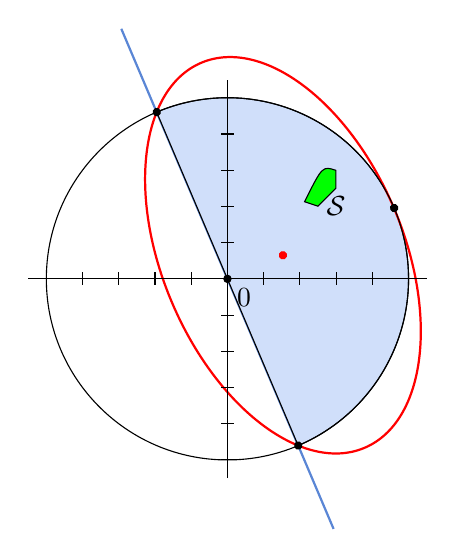
\begin{tikzpicture}[scale=2.3]

\begin{scope}[rotate=-157]
  \draw[draw=CornflowerBlue!90!black,thick] (0,-1.5) -- (0,1.5);
  \filldraw[ rotate=180, fill=CornflowerBlue!30, fill opacity=95] (0,-1) arc [start angle=-90, end angle=90, radius=1] -- cycle;
\draw[thick,draw=red] (-0.333,0) circle [x radius=0.666, y radius=1.1547];
\filldraw[red] (-0.333,0) circle [radius=0.02];

%\begin{scope}[shift={(-0.333,0)}]
%\draw[dashed, Salmon,  rotate=50] (0,-1.5) -- (0,1.5);
%\end{scope}

\filldraw (0,1) circle [radius=0.02];
\filldraw (0,-1) circle [radius=0.02] ;
\filldraw (-1,0) circle [radius=0.02] ;
\end{scope}
\filldraw[shift={(0.5,0.5)}, scale=0.07, rotate=45, draw=black, fill=green] 
      (-1,-1) -- (1,-1) -- (2,0) .. controls (1.5,1)  ..  (-1.5,0) -- cycle;
      \draw (0.6,0.4) node {$\cal S$};
\draw (0,0) circle [radius=1] node[anchor=north west] {$0$};
\filldraw (0,0) circle [radius=0.02];
%axis
\draw (-1.1,0) -- coordinate (x axis mid) (1.1,0);
\draw (0,-1.1) -- coordinate (y axis mid) (0,1.1);
%ticks
\foreach \x in {-1,-0.8,...,1}
\draw (\x,1pt) -- (\x,-1pt);
\foreach \y in {-1,-0.8,...,1}
\draw (1pt,\y) -- (-1pt,\y);

\end{tikzpicture}
\end{center}
\end{minipage}
\noindent  
  stred elipsy leží v $S$, 
  máme riešenie, inak 
  opäť existuje priamka prechádzajúca stredom elipsy tak, 
  že $S$ je v jednej polovici; môžeme nájsť najmenšiu
  elipsu opísanú príslušnej ''polelipse'' a takto pokračovať ďalej.
Pripomeňme, že elipsa $E$ so stredom v bode $(0,0)$ a jej plocha $\lVert E\rVert$ sú dané nasledovnými vzťahmi,
pričom $a$, $b$ sú dĺžky jednotlivých poloosí:

\begin{minipage}[t]{0.5\textwidth}
  \vskip 0pt
\begin{center}
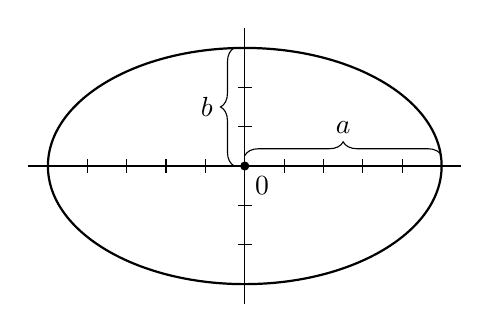
\begin{tikzpicture}[scale=2.5]

  \draw[thick] (0,0) ellipse (1.0 and 0.6)  node[anchor=north west] {$0$};
\filldraw (0,0) circle [radius=0.02];
%axis
\draw (-1.1,0) -- coordinate (x axis mid) (1.1,0);
\draw (0,-0.7) -- coordinate (y axis mid) (0,0.7);

 \draw [decorate,decoration={brace,amplitude=5pt,raise=5pt},xshift=0pt,yshift=-0.5pt] (0,0) -- (1,0)
  node[black,midway,yshift=15pt] {$a$};
 
  \draw [decorate,decoration={brace,amplitude=5pt,raise=5pt},xshift=0.5pt,yshift=0pt] (0,0) -- (0,0.6)
  node[black,midway,xshift=-15pt] {$b$};

%ticks
\foreach \x in {-1,-0.8,...,1}
\draw (\x,1pt) -- (\x,-1pt);
\foreach \y in {-0.6,-0.4,...,0.6}
\draw (1pt,\y) -- (-1pt,\y);


\end{tikzpicture}
\end{center}
\end{minipage}
\begin{minipage}[t]{0.5\textwidth}
  \vskip 0pt
  \begin{eqnarray*}
    E &=& \left\{ (x,y)\in\R^2\mid \frac{x^2}{a^2}+\frac{y^2}{b^2}\le1\right\} \\
    \lVert E\rVert & =& \pi a b
    \end{eqnarray*}
\end{minipage}


\noindent
Aby náš postup zafungoval, musíme vedieť nájsť najmenšiu elipsu opísanú generickej polelipse a ukázať, že jej plocha 
je o konštantný faktor menšia. Majme teda elipsu v ľubovoľnej polohe a priamku prechádzajúcu jej stredom. 
Začneme tým, že elipsu presunieme do bodu
$(0,0)$ a otočíme tak, aby jej osi boli rovnobbežné so súradnicovými osami. 


\begin{minipage}[t]{0.5\textwidth}
  \vskip 0pt
\begin{center}
\begin{tikzpicture}[scale=2.5]


\end{tikzpicture}
\end{center}
\end{minipage}
\begin{minipage}[t]{0.5\textwidth}
  \vskip 0pt
\begin{center}
\begin{tikzpicture}[scale=2.5]

\end{tikzpicture}
\end{center}
\end{minipage}


\IGNORE{
\vspace*{-4ex}
\noindent
\colorlet{shadecolor}{Aquamarine!9}
\begin{shaded}
\subsection*{Malá odbočka k elipsám}

\noindent
Čitateľ sa už možno stretol s konvexným obalom v dvoch rozmeroch: pre dané body
v rovine je ich konvexný obal najmenší konvexný mnohouholník, ktorý ich všetky obsahuje.

\end{shaded}



  elipsa opísaná polkruhu. Pozrime sa preto na elipsu trocha bližšie. Čitateľ si azda pamätá, že elipsa\footnote{% 
keď budeme hovoirť o elipse, vždy budeme myslieť elipsu aj s vnútrom} 
stredom v $[0,0]$ a poloosami $a$, $b$ je množina bodov $[x,y]$ v rovine, spĺňajúcich vzťah
$$\frac{x^2}{a^2}+\frac{y^2}{b^2}\le1$$
a jej plocha je $\pi ab$.

\begin{center}
\begin{tikzpicture}[scale=2.3]

% elipsa
\begin{scope} [rotate=-157]
\end{scope}


\end{tikzpicture}
\end{center}
}




% elipsoidova metoda
% bin packing (det. rounding)
%%, network design (iterative rounding), steiner tree (randomized rounding)
%% chernoff -multicomodity flow (random sampling)

% semidefinitne progr
% max cut

\IGNORE{
\chapter{Variácie na tému rezy}
V doterajšom texte sme si predstavili rôzne spôsoby, ako využiť optimalizačné metódy pri návrhu aproximačných
algoritmov. V nasledujúcich dvoch kapitolách si priblížime niektoré známe problémy a \ldots


Problém nájdenia minimálneho rezu v grafe, \mincut, by mal byť čitateľom dobre známy:

\begin{framed}
  \begin{dfn}
    \label{dfn:mincut}
    Majme daný jednoduchý graf $G=(V,E)$ s hranami ohodnotenými nezápornými váhami, t.j. funkciou
    $\omega:E\mapsto \R^+$ a v ňom dvojicu vrcholov $s,t$. Cieľom problému
    \mincut je odobrať z grafu $G$ množinu hrán s minimálnou celkovou váhou tak, aby
     vrcholy $s$ a $t$ neboli v rovnakom komponente súvislosti výsledného grafu.
  \end{dfn}
\end{framed}

Zaujímavá je spojitosť \mincut a \maxflow: známa veta hovorí, že veľkosti minimálneho rezu a maximálneho toku 
sú rovnaké. 


\begin{myfig}{\textwidth}{svg/flowcutNew}
  \centerline{Minimálny rez a maximálny tok sú rovnaké.}
\end{myfig}

Videli sme, že \maxflow sa dá vyjadriť ako lineárny program, ktorého duálny program
je relaxácia problému \mincut (v ktorej nevyberáme množinu hrán, ale každej hrane priradíme hodnotu
z intervalu $[0,1]$ a požadujeme, aby na každej $s-t$ ceste bol súčet hodnôt aspoň 1).
Zároveň, pretože matica obmedzení tohto relaxovaného programu je totálne unimodulárna, vieme,
že existuje celočíselné optimum. Efektívnu riešiteľnosť \mincut môžeme teda pripísať na vrub
špeciálnemu tvaru matice príslušného lineárneho programu. Dalo by sa očakávať, 
že programy takéhoto tvaru sú skôr výnimkou a pre väčšinu problémov podobná min-max charakterizácia
neplatí. V tomto texte chceme ilustrovať, že efektívne riešiteľné 
diskrétne optimalizačné problémy sú skôr výnimka ako pravidlo.
Prezentujeme niekoľko zovšeobecnení \mincut, ktoré sú \NP-ťažké
a ukážeme aproximačné algoritmy na ich riešenie.
Jedno zovšeobecnenie, v ktorom namiesto jednej dvojice vrcholov treba rozpojiť $k$ dvojíc, sme už videli:


\begin{framed}
  \begin{dfn}
    \label{dfn:multicut}
    Majme daný jednoduchý graf $G=(V,E)$ s hranami ohodnotenými nezápornými váhami, t.j. funkciou
    $\omega:E\mapsto \R^+$ a v ňom $k$ dvojíc vrcholov $(s_i,t_i)$, $i=1,\ldots,k$. Cieľom problému
    \minmulticut je odobrať z grafu $G$ množinu hrán s minimálnou celkovou váhou tak, aby
    žiadna dvojica $(s_i,t_i)$ nebola v rovnakom komponente súvislosti výsledného grafu.
  \end{dfn}
\end{framed}

a ukázali sme $4\ln(2k)$-aproximačný algoritmus. 

%%%%%%%%%%%%%%%%%%%%%%%%%%%%%%%%%%%%%%%%%%%%%%%%%%%%%%%%%%%%%%%%%%%%%%%%%%%%%%%%%%%%%%%%%%%%%%%%%%%%%%%%%%%%
\section*{Variácia prvá: \multiwaycut}

Iné zovšeobecnenie nepožaduje rozpojiť konkrétne dvojice vrcholov, ale iba rozdeliť 
niekoľko daných význačných vrcholov (terminálov) do rôznych komponentov súvislosti:

\begin{framed}
  \begin{dfn}
    \label{dfn:multiwaycut}
    Majme daný jednoduchý graf $G=(V,E)$ s hranami ohodnotenými nezápornými váhami, t.j. funkciou
    $\omega:E\mapsto \R^+$ a v ňom $k$  vrcholov $s_1,\ldots,s_k$. Cieľom problému
    \multiwaycut je odobrať z grafu $G$ množinu hrán s minimálnou celkovou váhou tak, aby
    žiadne dva vrcholy $s_i$, $s_j$  neboli v rovnakom komponente súvislosti výsledného grafu.
  \end{dfn}
\end{framed}

Bez ujmy na všeobecnosti môžeme predpokladať, že vstupný graf je súvislý (inak každý komponent
súvislosti môžme vyriešiť ako samostatnú inštanciu), a preto optimálne riešenie bude mať
práve $k$ komponentov (menej nemôže mať, lebo to by museli dva terminály byť v jednom komponente,
a viac nebude mať kvôli minimalite). 

\begin{myfig}{.6\textwidth}{svg/multiway1}
    Optimálne riešenie s cenou $43$. Platí
    $\partial(C_1)=21$,
    $\partial(C_2)=22$,
    $\partial(C_3)=1$,
    $\partial(C_4)=21$,
    $\partial(C_5)=1$,
  $\partial(C_6)=20$.
\end{myfig}


Označme $C_i$ komponent súvislosti optimálneho riešenia, ktorý obsahuje terminál $s_i$; nech
$\partial(C_i)$ je veľkosť rezu, ktorý oddeľuje komponent $C_i$, t.j.
\begin{equation}
  \label{eqn:cutedgeboundary}
  \partial(C_i):=\sum_{e=(u,v)\atop u\in C_i, v\not\in C_i} \omega(e).
\end{equation}

Cena optimálneho riešenia je potom 
\begin{equation}
  \label{eqn:multiwaycut:1}
  OPT=\frac{1}{2}\sum_{i=1}^k\partial(C_i),
\end{equation}

lebo každá hrana rezu je v sume na pravej strane zarátaná dvakrát.
Ukážeme si $2(1-\frac{1}{k})$-aproximačný algoritmus, t.j. algoritmus, ktorý vždy
nájde rez s hodnotou najviac $2(1-\frac{1}{k})$-násobku optima. 

Zoberme si ľubovoľný terminál $s_i$. 
Označme $D_i$ minimálny rez, ktorý oddeľuje $s_i$ 
od ostatných terminálov a označme $\partial(D_i)$ jeho veľkosť. 
Rez $D_i$ vieme pre každé $i$ vypočítať ľahko: všetky ostatné terminály zlúčime do jedného
vrchola a v takto získanom grafe zrátame minimálny rez.

\begin{minipage}[t]{0.45\textwidth}
  \vskip 0pt
\begin{myfig}{\textwidth}{svg/multiway2}
  \centerline{Rez $D_2$ má veľkosť 22.}
\end{myfig}
\end{minipage}
\hfill
\begin{minipage}[t]{0.45\textwidth}
  \vskip 0pt
\begin{myfig}{\textwidth}{svg/multiway3}
  Veľkosti rezov sú 
    $\partial(D_1)=20$,
    $\partial(D_2)=22$,
    $\partial(D_3)=1$,
    $\partial(D_4)=19$,
    $\partial(D_5)=1$,
    $\partial(D_6)=19$. Cena riešenia je $80$.
\end{myfig}
\end{minipage}

Čo sa stane, ak  za riešenie zoberieme zjednotenie rezov $D_1\cup D_2\cup\cdots\cup D_k$?
Každý rez $C_i$ z optimálneho riešenia oddeľuje $s_i$ od zvyšných terminálov. Keďže $D_i$ je minimálny
taký rez, je $\partial(D_i)\le\partial(C_i)$.
Zároveň pre cenu riešenia $m$ platí 
$$m\le\sum_{i=1}^k\partial(D_i)\le\sum_{i=1}^k\partial(C_i)=2\cdot OPT,$$
kde posledná rovnosť je (\ref{eqn:multiwaycut:1}), a preto máme 2-aproximačný algoritmus. Zároveň hneď vidíme,
ako ho trochu vylepšiť: prípustné riešenie dostaneme, ak urobíme zjednotenie hociktorých $k-1$ rezov  $D_i$ namiesto
všetkých $k$. Prirodzenou voľbou je vynechať ten najťažší; nech je to $D_j$. Keďže je najťažší, z Dirichletovho
princípu vyplýva, že musí byť aspoň tak ťažký ako priemer, t.j.
$$\partial(D_j)\ge\frac{1}{k}\sum_{i=1}^k\partial(D_i).$$
Pre cenu riešenia výsledného algoritmu potom dostávame
$$ALG\le\sum_{i=1\atop i\not=j}^k\partial(D_i)=\sum_{i=1}^k\partial(D_i)-\partial(D_j)\le
\left(1-\frac{1}{k}\right)\sum_{i=1}^k\partial(D_i)\le
\left(1-\frac{1}{k}\right)\sum_{i=1}^k\partial(C_i)=2\left(1-\frac{1}{k}\right) OPT.$$


%%%%%%%%%%%%%%%%%%%%%%%%%%%%%%%%%%%%%%%%%%%%%%%%%%%%%%%%%%%%%%%%%%%%%%%%%%%%%%%%%%%%%%%%%%%%%%%%%%%%%%%%%%%%
\section*{Variácia druhá: \kcut}

Poslednou variáciou v tomto texte je modifikácia problému \multiwaycut, pri ktorej nemáme žiadne terminály 
a chceme iba graf rozdeliť na (aspoň) $k$ častí:

\begin{framed}
  \begin{dfn}
    \label{dfn:kcut}
    Majme daný jednoduchý graf $G=(V,E)$ s hranami ohodnotenými nezápornými váhami, t.j. funkciou
    $\omega:E\mapsto \R^+$ a číslo $k$.
     Cieľom problému
    \kcut je odobrať z grafu $G$ množinu hrán s minimálnou celkovou váhou tak, aby
    výsledný graf mal aspoň $k$ komponentov súvislosti.
  \end{dfn}
\end{framed}

Podotýkame, že $k$ v názve problému je len symbol; počet častí, na ktoré treba rozkrájať graf, je súčasťou vstupu.
Opäť ide o \NP-ťažký problém a ukážeme si algoritmus s rovnakou garanciou aproximácie ako v predchádzajúcom prípade, 
t.j. $2\left(1-\frac{1}{k}\right)$. Predstavíme pri tom aj dátovú štruktúru, ktorá môže byť zaujímavá sama osebe.

\subsection*{Gomory-Hu stromy}

Predstavme si situáciu, že máme graf $G=(V,E)$ 
s hranami ohodnotenými nezápornými váhami  
a chceme pre každú dvojicu vrcholov $u,v$ zrátať cenu minimálneho $u-v$ rezu.
Priamočiary prístup je $\Omega(n^2)$-krát zavolať procedúru na výpočet minimálneho rezu.
Dá sa to ale aj lepšie: v skutočnosti nám stačí $O(n)$ počítaní minimálneho rezu. Kľúčom je
dátová štruktúra, ktorá efektívne kóduje minimálne rezy medzi všetkými dvojicami vrcholov, tzv.
Gomory-Hu strom. 

\vskip 1ex

V ďalšom budeme používať nasledovné označenie: 

\begin{itemize}
  \item Pre dva vrcholy $u,v\in V$, $f_G(u,v)$ (alebo
len $f(u,v)$ ak je $G$ zrejmé z kontextu), bude veľkosť minimálneho $u-v$ rezu v $G$. 
\item Ďalej,
nech $T=(V,E)$ je strom a $e\in E$ je hrana. Po jej odstránení dostaneme graf $T-\{e\}$, ktorý
má dva komponenty súvislosti. Označme $cut_T(e)\subseteq V$  
jeden\footnote{Aby sme mali jednoznačnú definíciu, potrebujeme povedať, ktorý komponent vyberieme.
  Keďže ale budeme hovoriť o veľkosti rezu medzi komponentami, 
  je nám to jedno. Napríklad nech $cut_T(e)$ je menší z komponentov $T-\{e\}$
  a v prípade rovnosti $cut_T(e)$ je 
ten komponent $T-\{e\}$, ktorý obsahuje nejaký pevne zvolený fixný vrchol $v_0$.}
z nich. 
\item Nech $G=(V,E)$ je graf. Tak ako v (\ref{eqn:cutedgeboundary}), 
  pre množinu $S\subseteq V$ bude $\partial_G(S)$ (resp. $\partial(S)$, ak je $G$ zrejmé)
veľkosť rezu určeného množinou $S$
(zjavne $\partial(S)=\partial(V-S)$).
\end{itemize}

\begin{framed}
  \begin{dfn}
    \label{dfn:GomoryHu}
    Majme daný jednoduchý graf $G=(V,E)$ s hranami ohodnotenými nezápornými váhami, t.j. funkciou
    $\omega:E\mapsto \R^+$. {\em Gomory-Hu strom} ku grafu $G$ je strom $T=(V,E')$, s hranami
    ohodnotenými funkciou  $\omega':E'\mapsto \R^+$, ktorý spĺňa tieto vlastnosti:
    \begin{enumerate}
      \item $\forall e'\in E':\;\omega'(e')=\partial_G(cut_T(e'))$
      \item $\forall u,v\in V:\;f_G(u,v)=f_T(u,v)$
    \end{enumerate}
  \end{dfn}
\end{framed}

Definícia~\ref{dfn:GomoryHu} nehovorí, ako taký strom skonštruovať (ani nehovorí, či je jednoznačný), ale iba
to, že každý strom s danými vlastnosťami je Gomory-Hu strom. Čo vlastne v Definícii~\ref{dfn:GomoryHu} požadujeme?
Strom $T$ má rovnakú množinu vrcholov ako $G$, ale hrany môže mať úplne iné (nijak nesúvisia s hranami $G$).
Prvá vlastnosť hovorí, že ak by sme už poznali hrany $E'$, ich váhy $\omega'$ vyrátame ľahko: pre každú
hranu $e'$ sa pozrieme, na aké množiny sa rozpadne $T$ po odobratí $e'$, a potom zrátame veľkosť
rezu v $G$ medzi týmito množinami. Napríklad na nasledujúcom obrázku je $cut_T((j,c))=\{c,d\}$
a $\partial_G(\{c,d\})=20$ (z množiny $\{c,d\}$ odchádzajú hrany $(b,c)$ a $(e,c)$).


\begin{myfig}{\textwidth}{svg/kcut1}
  \centerline{Graf $G$ a jeho Gomory-Hu strom $T$.}
\end{myfig}


Druhá vlastnosť hovorí, že z $T$ sa dajú vyčítať hodnoty minimálneho rezu medzi ľubovoľnými dvoma vrcholmi:
$f_G(u,v)$, teda veľkosť minimálneho $u-v$ rezu v $G$, je $f_T(u,v)$: $T$ je strom, takže obsahuje práve jednu
$u-v$ cestu, a preto $f_T(u,v)$ je minimálna váha $\omega'$ na tejto ceste. Napríklad pre vrcholy $a,k$ na obrázku
je v $T$ cesta $a-b-j-k$ a $f_T(a,k)=20$. Minimum sa nadobúda na hrane $a-b$ a $cut_T((a,b))=\{a\}$. Vskutku,
rez $\{a\}$ s $\partial_G(\{a\})=20$ (kvôli hranám $(a,b)$, $(a,j)$) je minimálny $a-k$ rez v $G$.

\vskip 2ex

Poďme teraz ukázať algoritmus, ktorý vyrobí k danému grafu $G$ jeho Gomory-Hu strom. 
Bude postupovať v iteráciách, pričom v každej iterácii $t$ bude mať
partíciu vrcholov $V=S^{(t)}_1\cup S^{(t)}_2\cup\cdots\cup S^{(t)}_{n_t}$, 
pričom $S^{(t)}_i\cap S^{(t)}_j=\emptyset$ 
pre $i\not=j$. Množiny $S^{(t)}_i$ budeme volať krabice. Na začiatku sú všetky vrcholy v jednej krabici,
t.j. $n_0=1$, $S^{(0)}_1=V$. 
Na konci chceme, aby každá krabica obsahovala jeden vrchol; po skončení algoritmu môžeme preto
jednoprvkové krabice stotožniť s príslušnými vrcholmi.

Na začiatku iterácie $t+1$ sú krabice
pospájané stromom $T^{(t)}=\left(\left\{S_i^{(t)}\right\}_{i=1}^{n_t},E^{(t)}\right)$ s ohodnotenými hranami. Iterácia $t+1$
zoberie jednu krabicu $S=S^{(t)}_i$ a zakorení $T^{(t)}$ v $S$. Vyberie z $S$ dva vrcholy $x,y$
a rozdelí $S$ na dve krabice $S_x$ a $S_y$ spojené hranou, pričom zvolí váhu pre novú hranu a
vhodne prerozdelí podstromy.
Cieľom je implementovať rozdeľovanie krabíc a prerozdeľovanie podstromov tak, aby po skončení algoritmu bol strom $T$
Gomory-Hu strom pre graf $G$.

\begin{myfig}{0.75\textwidth}{svg/kcut2}
\end{myfig}

Počas behu algoritmu bude platiť nasledovný invariant:

\begin{framed}
{\bf Invariant:} Nech $e\in E^{(t)}$ je ľubovoľná hrana v strome $T^{(t)}$, $e=\left(S_i^{(t)},S_J^{(t)}\right)$,
potom $cut_{T^{(t)}}(e)$ je množina krabíc v jednom komponente $T^{(t)}-\{e\}$. Nech $M$
sú vrcholy grafu $G$ z týchto krabíc, t.j. $M:=\{v\in V\mid \exists S\in cut_{T^{(t)}}(e):\;v\in S\}$.
Potom existujú dvaja {\em svedkovia} $x\in S_i^{(t)}$, $y\in S_j^{(t)}$, že $\omega'(e)=f_G(x,y)$ a 
$M$ je minimálny $x-y$ rez v $G$.
\end{framed}

Inými slovami, keď si zoberieme hocijakú hranu $e$ zo stromu krabíc, vieme jej priradiť rez v grafe $G$: rez je
definovaný množinou tých vrcholov z $V$, ktoré sú v niektorej krabici z jedného komponentu $T^{(t)}-\{e\}$.
Tento rez v $G$ musí byť minimálny $x-y$ rez pre svedkov $x,y$, a zároveň cena hrany $e$ v strome $T^{(t)}$
musí byť cena tohoto rezu.

Teraz potrebujeme urobiť dve veci: jednak ukázať, že keď algoritmus skončí a platí invariant, máme dobrý 
Gomory-Hu strom a dvak navrhnúť iteráciu algoritmu tak, aby invariant ostával v platnosti.

Najprv si ukážeme, že ak platí invariant a každá krabica je jednoprvková, máme Gomory-Hu strom. 
Nech $T=(V,E')$ je strom po skončení algoritmu a nech v ňom platí invariant. Keďže každá krabica bola jednoprvková,
svedkovia z invariantu sú samotné vrcholy.
Potrebujeme ukázať
obe vlastnosti z Definície~\ref{dfn:GomoryHu}. Prvá vlastnosť, $\omega'(e)=\partial_G(cut_T(e))$,  hovorí, 
že váha hrany $e\in E'$ je cena príslušného rezu v $G$. Z invariantu ale platí, že $cut_T(e)$ je minimálny
$x-y$ rez, kde $e=(x,y)$. Zároveň invariant hovorí, že $\omega'(e)=f_G(x,y)=\partial_G(cut_T(e))$.
Prvá vlastnosť z Definície~\ref{dfn:GomoryHu} je preto splnená. 

Druhá vlastnosť hovorí, že $f_G(u,v)=f_T(u,v)$
pre ľubovoľné dva vrcholy $u,v\in V$. Ak $(u,v)\in E'$, vlastnosť vyplýva priamo z invariantu:
keďže $u,v$ sú spojené hranou v strome $T$, je $f_T(u,v)=\omega'((u,v))=f_G(u,v)$.
Nech teda $u,v$ nie sú spojené hranou v $T$. Keďže $T$ je strom, je v ňom práve jedna $u-v$ cesta
$u=w_0,w_1,\ldots,w_z=v$ a minimálny $u-v$ rez v $T$ je hrana s minimálnou váhou na nej.
Označme túto hranu $e_{\min}=(w_i,w_{i+1})$, t.j. chceme ukázať $f_G(u,v)=\omega'(e_{\min})$.

Na jednej strane, v $T-\{e_{\min}\}$ sú $w_{i}$ a $w_{i+1}$ v rôznych komponentoch, a teda aj $u$ a $v$
sú v rôznych komponentoch. Preto $cut_T(e_{\min})$ je rez v $G$, ktorý oddelí $u$
od $v$, a teda $\partial_G(cut_T(e_{\min}))\ge f_G(u,v)$. Z predchádzajúcich úvah ale vieme,
že $\partial_G(cut_T(e_{\min}))=\omega'(e_{\min})$, a tak sme ukázali, že $\omega'(e_{\min})\ge  f_G(u,v)$.

\begin{myfig}{\textwidth}{svg/kcut3}
  Vľavo je graf $G=(V,E)$, vpravo jeho Gomory-Hu strom $T$. Medzi vrcholmi $u$, $v$ je v $T$ jediná cesta
a na nej je hrana $e_{\min}$. Odstránením hrany $e_{\min}$ z $T$ dostaneme rozklad $V$ na dve množiny,
a teda rez v $G$. Vieme, že cena hrany $e_{\min}$ v $T$ je veľkosť minimálneho rezu $G$ medzi
koncovými vrcholmi $e_{\min}$. Teraz sa pokúšame ukázať, že tento rez je zároveň minimálny $u-v$ rez.
\end{myfig}


Na to, aby sme ukázali opačnú nerovnosť, t.j. $\omega'(e_{\min})\le  f_G(u,v)$, si pomôžeme nasledovnou lemou:

\begin{lema}
  \label{lm:kcutreclema}
  Majme graf $G=(V,E)$ a nech $\{v_1,v_2,\ldots,v_z\}\subseteq V$. Potom
  $$f_G(v_1,v_z)\ge\min\{f_G(v_1,v_2),f_G(v_2,v_3),\ldots,f_G(v_{z-1},v_z)\}.$$
\end{lema}

\begin{dokaz}
  Urobíme indukciu na $z$. Pre $z=2$ lema triviálne platí. Ak $z>2$, z indukčného predpokladu vieme,
  že $f(v_2,v_z)\ge\min\{f(v_2,v_3),\ldots,f(v_{z-1},v_z)\}$. Preto nám stačí ukázať, že
  $f(v_1,v_z)\ge\min\{ f(v_1,v_2), f(v_2,v_z) \}$. Predpokladajme sporom, že 
  $f(v_1,v_z)<\min\{ f(v_1,v_2), f(v_2,v_z) \}$ a nech $C$ je minimálny $v_1-v_z$ rez v $G$. 
  Bez ujmy na všeobecnosti, nech
   $v_2$
   je na rovnakej strane rezu, ako $v_1$ (ináč premenujeme $v_1$ a $v_z$ a máme symetrickú situáciu).
  $C$ je zároveň $v_2-v_z$ rez, a preto
  $f(v_2,v_z)\le f(v_1,v_z)$, spor.
\end{dokaz}

Teraz vieme, že $f_G(u,v)\ge\min\{f_G(w_0,w_1),f_G(w_1,w_2),\ldots,f_G(v_{z-1},w_z)\}.$
Zároveň, pretože $(w_i,w_{i+1})\in E'$, z predchádzajúcich úvah vieme, že 
$f_G(w_i,w_{i+1})=\omega'((w_i,w_{i+1}))$, a teda
$$f_G(u,v)\ge\min\{\omega'(w_0,w_1),\ldots,\omega'(w_{z-1},w_z)\}=\omega'(e_{\min}).$$

\vskip 2ex
Teraz, keď už vieme, že ak po skončení algoritmu invariant platí, tak máme dobrý Gomory-Hu strom,
poďme navrhnúť algoritmus tak, aby invariant ostával v platnosti. Ako sme už povedali, v jednej iterácii
si algoritmus vyberie krabicu $S$ (ľubovoľnú) s aspoň dvoma vrcholmi $x$ a $y$ (ľubovoľnými) a rozdelí
$S$ na dve menšie krabice. Toto rozdelenie sa urobí takto: zakoreníme strom $T^{(t)}$ v  $S$ 
 a nech
$T_1,\ldots,T_z$ sú podstromy synov $S$. Pre podstrom $T_i$ označme $V_i$ tie vrcholy grafu $G$, ktoré
sú v niektorej krabici z tohto podstromu, t.j. $V_i:=\{v\in V\mid \exists S'\in T_i:\;v\in S'\}$.
Z $G$ zostrojíme graf $G'$ tak, že vrcholy z $V_i$ sa stotožnia a nahradia sa novým vrcholom $y_i$,
pričom hrany ostanú (t.j. nový graf môže mať násobné hrany). V grafe $G'$ 
nájdeme minimálny $x-y$ rez $T$. Krabicu $S$ nahradíme dvoma krabicami $S_x:=S\cap T$, $S_y:= S-S_x$.
Do stromu pridáme hranu spájajúcu $S_x$ a $S_y$ s cenou $\partial_G(T)$. Podstromy $T_i$, pre ktoré
$y_i\in T$, budú susediť s $S_x$, zvyšné podstromy s $S_y$.


\begin{myfig}{\textwidth}{svg/kcut4}
  Vľavo je stav na začiatku iterácie: máme štyri krabice pospájané hranami do stromu (modré
  čísla sú váhy $\omega'$ v $T^{(t)}$, čierne sú pôvodné váhy $\omega$ v $G$).
  Jednu krabicu $S$ sme vybrali za koreň a vybrali dva ľubovoľné vrcholy $x,y\in S$.
  $S$ má dvoch synov a príslušné podstromy skontrahujeme do dvoch vrcholov; dostaneme tak graf vpravo,
  v ktorom nájdeme minimálny $x-y$ rez $T$. 
\end{myfig}



\begin{myfig}{\textwidth}{svg/kcut5}
Nájdený rez jednak definuje, ako rozdeliť $S$ na $S_x$ a $S_y$, a zároveň určuje, ktorý podstrom bude kam patriť.
\end{myfig}

Na záver rozprávania o Gomory-Hu stromoch potrebujeme ukázať, že takto definovaný spôsob rozbíjania krabíc
zachováva v platnosti invariant, teda že ak na začiatku iterácie invariant platil, bude platiť aj po jej skončení.
Zjavne pre hrany stromu, ktoré sú v niektorom podstrome $T_i$, sa počas iterácie nič nezmenilo: svedkovia ostali,
váha hrany aj rez ňou definovaný sa taktiež nezmenili. Pre hrany, ktoré v pôvodnom strome boli incidentné s $S$
sa nezmenila váha, ani hodnota rezu, ale mohlo sa stať, že po rozdelení $S$ sa jeden svedok stratil a budeme
musieť nájsť iného. Napokon
treba ukázať platnosť invariantu pre novú hranu $(S_x,S_y)$. 
V tom všetkom nám viackrát pomôže nasledovná lema:

\begin{lema}
  \label{lm:kcutlema}
  Majme graf $G=(V,E)$ a nech $S\subseteq V$ je nejaký minimálny $r-s$ rez pre $r,s\in V$, pričom $s\in S$.
  Ďalej, nech $v,w\in S$ sú dva ľubovoľné vrcholy. Potom existuje minimálny $v-w$ rez $T$ v $G$ taký, že 
  $T\subset S$.
\end{lema}

\begin{dokaz}
  Zoberme si nejaký minimálny $v-w$ rez $X$. Ak $X\subset S$ (alebo $V-T\subset S$), niet čo dokazovať.
  Takže predpokladajme, že $S\cap X\not=\emptyset$ a uvažujme výraz $A:=\partial(S)+\partial(X)$. 
  Podľa príslušnosti koncových vrcholov do $S$ a $X$ máme 6 typov hrán, ktoré prispievajú do $A$.
  V nasledujúcom obrázku je pre každý typ hrán uvedená násobnosť, t.j. napríklad každá z hrán medzi $S-X$ a $X-S$
  je zarátaná dvakrát (raz v $\partial(S)$ a raz v $\partial(X)$), každá z hrán medzi $S-X$ a $S\cap X$ 
  sa zarátava raz (v $\partial(X)$)  atď.

  \begin{myfig}{0.4\textwidth}{svg/kcut6}
  \end{myfig}

  \vspace*{-6ex}
  Rozlíšme teraz dva prípady: 

  {\bf 1. $r\in X$.} Budeme uvažovať výraz $B:=\partial(S-X)+\partial(X-S)$ a podobne ako pre výraz $A$, 
  aj teraz sa pozrime, ktoré hrany sa koľkokrát započítajú:
  
  \begin{myfig}{0.4\textwidth}{svg/kcut7}
  \end{myfig}
  \vspace*{-6ex}

  Porovnaním počtov zarátaných hrán vidíme, že $B\le A$, t.j.
  $$\partial(S-X)+\partial(X-S)\le\partial(S)+\partial(X).$$
  Zároveň, pretože $s\in S$,  $X-S$ je $r-s$ rez, a keďže
  $S$ je minimálny $r-s$ rez, platí $\partial(X-S)\ge\partial(S)$.
  Odtiaľ potom dostávame $\partial(S-X)\le\partial(X)$. Lenže $X$ aj $S-X$ sú $v-w$ rezy, a navyše $X$ je minimálny
  $v-w$ rez. Preto  $S-X$ je minimálny $v-w$ rez, pre ktorý platí $S-X\subset S$.


  \vskip 1ex
  {\bf 2. $r\not\in X$.} Postup bude analogický ako v predchádzajúcom prípade, iba teraz budeme uvažovať výraz
  $B':=\partial(S\cup X)+\partial(S\cap X)$.
  
  \begin{myfig}{0.4\textwidth}{svg/kcut8}
  \end{myfig}

  \vspace*{-6ex}
  Porovnaním opäť vidíme $B'\le A$, t.j.
  $$\partial(S\cup X)+\partial(S\cap X)\le\partial(S)+\partial(X).$$
  Pretože $r\not\in S\cup X$, je $S\cup X$ $r-s$ rez, a preto $\partial(S\cup X)\ge\partial(S)$. 
  Z predchádzajúcej nerovnosti potom máme $\partial(S\cap X)\le\partial(X)$, takže $S\cap X$ je minimálny
  $v-w$ rez obsiahnutý v $S$.
\end{dokaz}

Majme teraz jednu iteráciu Gomory-Hu algoritmu, ktorá rozdelila krabicu $S$ na krabice $S_x$ a $S_y$.
Ukážeme, že pre novú hranu $e'=(S_x,S_y)$ platí invariant. Rez definovaný hranou $e'$ je rez, ktorý vznikol
z minimálneho $x-y$ rezu v $G'$ a $\omega'(e')$ je jeho cena. Stačí nám teda ukázať, že minimálny $x-y$ rez v $G'$
je zároveň (po expandovaní vrcholov $y_i$) minimálny $x-y$ rez v $G$; inými slovami, minimálny $x-y$ rez v $G$
nerozdelí vrcholy patriace do jedného podstromu $T_i$.

Nech $K_1,\ldots,K_z$ sú synovia $S$ (t.j. korene podstromov $T_1,\ldots,T_z$) a 
nech $a_i\in K_i$, $s_i\in S$ sú príslušní svedkovia. 
Hrana $(S,K_1)$ definuje rez v $G$, 
v ktorom na jednej strane sú vrcholy podstromu $T_1$, na druhej strane všetky ostatné vrcholy, vrátane $x$ a $y$.
Pretože tento rez je zároveň minimálny $a_1-s_1$ rez, z Lemy~\ref{lm:kcutlema}
dostaneme, že v $G$ existuje $x-y$ rez, ktorý nerozdelí vrcholy podstromu $T_1$. 
Iterovaním tohto argumentu pre ostatné podstromy dostaneme požadované tvrdenie.

\begin{minipage}[t]{0.3\textwidth}
  \vskip 0pt
  \begin{myfig}{\textwidth}{svg/kcut9}
  \end{myfig}
\end{minipage}\hfill
\begin{minipage}[t]{.6\textwidth}
  \vskip 0pt
Posledná vec, ktorú potrebujeme ukázať, sa týka hrán $(S,K_i)$. Na začiatku iterácie boli svedkovia
$a_i\in K_i$, $s_i\in S$, ktorí dosvedčili platnosť invariantu. Bez ujmy na všeobecnosti, nech
po skončení iterácie sa z hrany $(S,K_i)$ stala hrana $(S_x,K_i)$. Ak $s_i\in S_x$, invariant 
zjavne ostáva v platnosti. Mohlo sa ale stať, že $s_i\in S_y$.
V tom prípade zoberieme za nového svedka $x$ a ukážeme, že $f_G(a_i,x)=f_G(a_i,s_i)$.

Na jednej strane, pretože rez definovaný hranou $(S,K_i)$ je minimálny $a_i,s_i$ rez v $G$, a zároveň
oddeľuje $a_i$ od $x$, platí $f_G(a_i,x)\le f_G(a_i,s_i)$.
\end{minipage}

Aby sme ukázali opačnú nerovnosť, vyrobme z $G$  pomocný graf $\hat{G}$, 
v ktorom skontrahujeme $S_y$ do jedného vrchola $\hat{y}$. Pretože $S_x$ a $S_y$ vznikli podľa minimálneho $x-y$ rezu,
môžme použiť Lemu~\ref{lm:kcutlema} a argumentovať, že $f_G(a_i,x)=f_{\hat{G}}(a_i,x)$.
Zároveň z Lemy~\ref{lm:kcutreclema} vieme, že $f_{\hat{G}}(a_i,x)\ge\min\{f_{\hat{G}}(x,\hat{y}), 
f_{\hat{G}}(a_i,\hat{y})\}$.
Z minimálneho $a_i-\hat{y}$ rezu v $\hat{G}$ expandovaním $\hat{y}$ vznikne nejaký  $a_i-s_i$ rez v $G$, a preto
$f_{\hat{G}}(a_i,\hat{y})\ge f_G(a_i,s_i)$.
Z rovnakých dôvodov platí $f_{\hat{G}}(x,\hat{y})\ge f_G(x,y)$; zároveň ale minimálny $x-y$ rez v $G$
oddeľuje $a_i$ a $s_i$, preto $f_G(x,y)\ge f_G(a_i,s_i)$, takže aj $f_{\hat{G}}(x,\hat{y})\ge f_G(a_i,s_i)$.

\subsection*{Naspäť k \kcut}

Uvažujme nasledovný jednoduchý algoritmus: pre daný graf $G=(V,E)$ zostroj Gomory-Hu strom $T$.
Zober $k-1$ najlacnejších hrán z $T$, $T$ sa tak rozpadne na $k$ súvislých komponentov. Tieto
komponenty vráť ako riešenie problému \kcut.
Ukážeme, že tento algoritmus je $2\left(1-\frac{1}{k}\right)$-aproximačný.

Nech hrany $T$ majú váhy $\omega'(e'_1)\le\omega'(e'_2)\le\cdots\le\omega'(e'_{n-1})$ a nech
$C_1,\ldots,C_k$ sú komponenty súvislosti optimálneho riešenia, pričom 
$\partial(C_1)\le\partial(C_2)\le\cdots\le\partial(C_k)$.
Z definície Gomory-Hu stromu, $\omega'(e'_i)=\partial_G(cut_T(e'))$, t.j. cena hrany v $T$ je cena
príslušného rezu v $G$. Keďže
algoritmus zoberie zjednotenie prvých $k-1$ rezov, môže sa stať, že niektoré hrany patria do viacerých
rezov, ale v každom prípade pre cenu algoritmu platí $ALG\le\sum_{i=1}^{k-1}\omega'(e'_i)$.
Na druhej strane, pre cenu optimálneho riešenia platí $2\cdot OPT=\sum_{i=1}^k\partial_G(C_i)$. Naším 
cieľom bude nájsť nejakých $k-1$ hrán v $T$ tak, že $i$-ta nájdená hrana má cenu nanajvýš $\partial_G(C_i)$.
Ak sa nám to podarí, budeme vedieť, že $ALG\le\sum_{i=1}^{k-1}\partial_G(C_i)$, lebo algoritmus
vyberá $k-1$ najlacnejších hrán z $T$. Zvyšné argumenty sú potom rovnaké ako v prípade \multiwaycut.

Zoberme si strom $T$ a skontrahujme každý komponent $C_i$ do jedného vrchola. Takto vzniknutý graf $T'$ môže mať 
cykly aj násobné hrany.

\begin{myfig}{0.9\textwidth}{svg/kcut10}
\end{myfig}

Vyhoďme z $T'$  hrany tak, aby ostal strom $T''$  a zakoreňme ho v $C_k$.
Pre každý vrchol $C_i$, $i=1,\ldots,k-1$ zoberme hranu $e'_{h_i}$, 
ktorá ide k jeho rodičovi v $T''$; dostali sme $k-1$ hrán z $T$. Ukážeme, že $\omega'(e'_{h_i})\le\partial_G(C_i)$,
čím sa celý dôkaz skončí.
Hrana $e'_{h_i}=(u,v)$ má jeden koncový vrchol v $C_i$ a druhý mimo $C_i$. $\omega'(e'_{h_i})$ je cena
minimálneho $u-v$ rezu v $G$. Ale $C_i$ tiež oddeľuje $u$ od $v$, a preto $\omega'(e'_{h_i})\le\partial_G(C_i)$.



}
%\chapter{Problém obchodného cestujúceho}

%\chapter{Neaproximovateľnosť}


%%
%treba:  determinanty, matice, stredna hodnota, nahodne premenne, ag nerovnost, derivacie

%%%%%%%%%%%%%%%%%%%%%%%%%%%%%%%%%%%%%%%%%%%%%%%%%%%%%%%%%%%%%%%%%%%%%%

%\vfill
%\centerline{  * * * TO BE CONTINUED ... * * * }
%\vfill

